\chapter{Application Development and Implementation}

\section{Database Design}
In this phase of development, the first priority is designing the database to handle mood data from university students. The database is the foundation of the entire application, as it manages all the core data related to users, surveys, questions, answers, and interactions. A solid and well designed database structure ensures efficient data handling, retrieval, and storage, which is crucial for performance and scalability.

\subsection{Entity-Relationship Diagram (ERD)}

To begin with, I used \textbf{\href{https://erdmaker.com/}{ERD Maker}}\footnote{Link: \url{https://erdmaker.com/}} to visualize and design the ERD for the application. First of all, we need to define the foundations of the ERD, so we can undestand and use them during the designing process. \vspace{5mm} \\
Each \textbf{Entity} is represented by a rectangular box, while each \textbf{Relationship} is depicted with a diamond. Every entity includes \textbf{Attributes}, which are represented by ellipses and describe the properties of each object within the entity.\vspace{5mm} \\
Each Entity is usually uniquely identified by one or more of its attributes, which are unique and are called the \textbf{Primary Key} of the entity. The attributes that contain a primary key are underlined within the ellipse.\vspace{5mm} \\
A \textbf{Relationship} describes the connection between two or more entities. The ``cardinality'' of the relationship specifies the number of instances of one entity that are associated with another entity through the relationship. A relationship can also include attributes that describe the properties of the connection between objects of the included entities. The cardinality on each side of the relationship can take the following values:
\begin{itemize}
    \item \textbf{0 to 1}: At most one instance of the entity is required for the relationship.
    \item \textbf{1 to 1}: Exactly one instance of the entity is required for the relationship.
    \item \textbf{0 to many}: Any number of instances of the entity can participate in the relationship.
    \item \textbf{1 to many}: At least one instance of the entity is required for the relationship.
\end{itemize}

\noindent A \textbf{Weak Entity} is an entity that cannot be uniquely identified by its own attributes alone. Instead, it relies on a \textbf{Strong Entity} (or parent entity) to define its uniqueness. This type of entity is typically used when an object’s existence depends on another object. In ER diagrams, a weak entity is represented by a double-lined rectangular box, and its relationship with the strong entity, known as a \textbf{Weak Relationship} (Non-Identifying), is depicted by a double-lined diamond. The weak entity is uniquely identified by a combination of its own attributes and the primary key of the strong entity.\vspace{5mm} \\
The ERD of the application is shown below:

\vspace{5mm}

\FloatBarrier
\begin{figure}[ht]
    \centering
    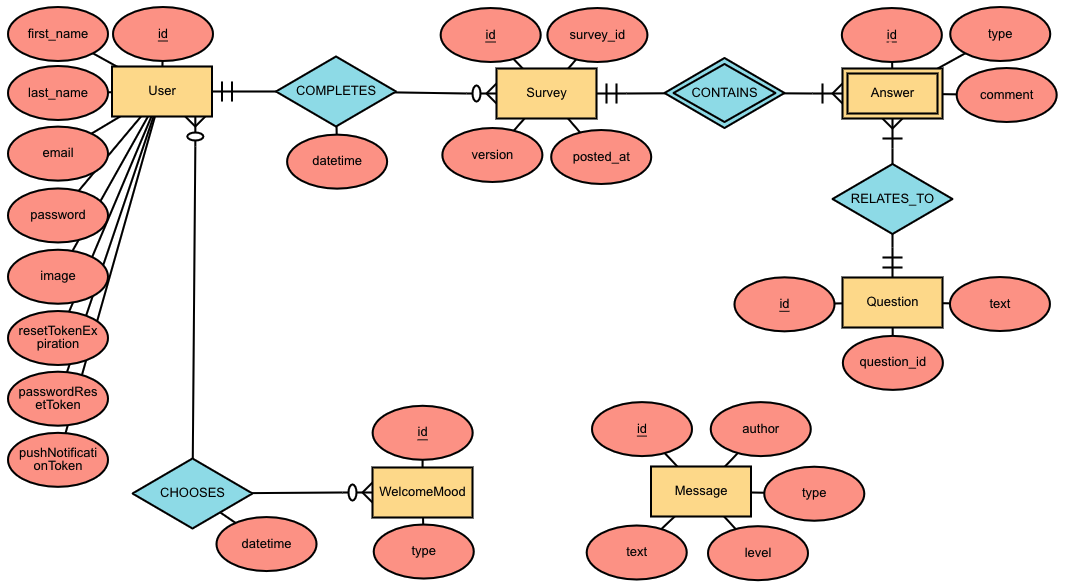
\includegraphics[width=\linewidth]{figures/database/ERD.png}
    \label{fig:erd}
    \caption{ERD}
\end{figure}
\FloatBarrier

\vspace{5mm}

\noindent Now, we proceed by providing a detailed explanation of the ERD, including the entities and their relationships. This clarifies the structure and logic behind the database design.

\subsection{Entities}
The core entities used in this project are \textbf{User}, \textbf{Survey}, \textbf{Answer}, \textbf{Question}, \textbf{Welcome Mood}, and \textbf{Message}. The first step in designing the database is to assign a unique identifier (ID) to each entity. This ensures that every instance within each entity is uniquely identifiable and makes efficient relationships and communication between entities possible. With the ID in place, we describe each entity in detail, starting with the most important entity in the ERD, the ``User'' entity, which serves as the foundation of the entire system.

\vspace{5mm}

\noindent \textbf{User} \\
The User entity is the central component of the application, as all other entities and processes revolve around the user. The following attributes are defined to ensure that we capture all necessary information for each user:

\begin{itemize}
    \item \textbf{id}
    \item \textbf{first\_name}: Captures the first name of the user. This is important for personalizing the user experience and identifying the user within the system.
    \item \textbf{last\_name}: Stores the user's last name, adding further personal identification.
    \item \textbf{email}: This attribute stores the user's email address, which is necessary for account creation, login, and any form of communication with the user.
    \item \textbf{password}: The password is securely stored to authenticate users during login. It ensures that only authorized individuals can access their account and related data.
    \item \textbf{image}: This optional attribute stores a link to the user’s profile picture, enhancing user personalization within the application.
    \item \textbf{resetTokenExpiration} and \textbf{passwordResetToken}: These attributes manage the password reset functionality. They store the reset token and its expiration, allowing users to securely reset their passwords if needed.
    \item \textbf{pushNotificationToken}: Stores the token required to send push notifications to the user's device, ensuring users receive timely updates and reminders from the application.
\end{itemize}

\noindent In addition to these attributes, two core features of the application depend on the user: the ``Survey'' process and the ``Welcome Mood'' process, both of which are discussed in detail below.

\vspace{5mm}

\noindent \textbf{Survey} \\
The Survey entity represents the surveys that users participate in. Surveys are a key feature in tracking the user's mood and well-being over time. The following attributes are defined for the entity:

\begin{itemize}
    \item \textbf{id}: This is an integer that identifies each survey session of a user. It simplifies referencing individual surveys and allows for tracking the number of surveys a user completes over time. Both the ``id'' attibute and the ``part'' attribute that we mention afterwards, make the unique key of the Survey entity.
    \item \textbf{part}: Specifies the part of the survey. This is particularly useful for distinguishing between the three predefined parts of the survey.
    \item \textbf{posted\_at}: Stores the timestamp when the survey was made available to the user. This helps in tracking when a survey was taken and how frequently the user engages with surveys.
\end{itemize}

\noindent By defining both \textbf{id} and \textbf{part}, we stick to the original plan, which was to have three distinct part of the survey for users to complete over a three-day period. After the third day, the cycle restarts with the first part. The \textbf{part} attribute takes values of 1, 2, and 3 to represent the three unique survey variations, while the \textbf{id} increments continuously (1, 2, 3, 4, and so on) to track each individual survey session.\vspace{5mm} \\
This structure aligns with the concept outlined during the UI/UX design phase, where a user completes three different parts of the survey over three consecutive days. Together, these parts form a complete survey cycle, which in turn contributes to completing the full questionnaire.

\vspace{5mm}

\noindent \textbf{Answer} \\
The Answer entity stores the responses provided by users to the survey questions. Each answer is linked to both a ``Survey'' and a ``Question'', forming a critical part of the survey process. The following attributes are defined for the `Answer` entity:

\begin{itemize}
    \item \textbf{id}
    \item \textbf{type}: Defines the type of response, with values of ``Not True'', ``Sometimes'', or ``True'', ensuring alignment with the structure of the questionnaire.
    \item \textbf{comment}: This optional attribute allows users to add comments or explanations to their answers, providing deeper insights alongside the structured survey responses.
\end{itemize}

\vspace{5mm}

\noindent \textbf{Question} \\
The Question entity holds the questions that appear in the surveys. Since the questions are fixed and don't change across surveys, the following attributes are defined:

\begin{itemize}
    \item \textbf{id}: An integer that identifies each question. It is used for easier referencing and troubleshooting, particularly when assigning questions to their respective survey parts.
    \item \textbf{text}: This contains the actual question text that is presented to the user.
\end{itemize}

\vspace{5mm}

\noindent \textbf{WelcomeMood} \\
The WelcomeMood entity tracks the welcome moods that users can select when they first interact with the application (in the ``Welcome Screen''). The selection of welcome mood helps tailor the user experience. The following attributes are defined:

\begin{itemize}
    \item \textbf{id}
    \item \textbf{type}: Defines the type of welcome mood (e.g., awful, sad, neutral, etc.). This is essential for categorizing user welcome moods and allowing the application to offer personalized content or feedback based on the user's current mood.
\end{itemize}

\vspace{5mm}

\noindent \textbf{Message} \\
The Message entity is used to store quotes or advice that is shown to users based on their overall mood level. These messages serve as a form of communication between the system and the user, providing motivational content that aligns with the user's emotional state. The following attributes are defined:

\begin{itemize}
    \item \textbf{id}
    \item \textbf{type}: This indicates whether the message is a ``quote'' or ``advice'', helping to categorize the content for appropriate usage.
    \item \textbf{author}: This attribute stores the name of the author of the message. If the author is known, their name is recorded; otherwise, the message is saved as ``Anonymous''.
    \item \textbf{level}: This attribute takes values of ``bad'', ``mid'', or ``good'', corresponding to the overall mood level of the user. The level determines which message is shown based on the user’s current emotional state.
    \item \textbf{text}: Contains the actual text of the message, either a quote or advice that is presented to the user.
\end{itemize}

\vspace{10mm}

\noindent By defining these entities and their respective attributes, we can effectively structure the database to support the main functionalities of the application. This approach ensures that the data model is optimized for managing user interactions, surveys and mood tracking.

\subsection{Relationships}
The core relationships used in this project are \textbf{COMPLETES}, \textbf{CONTAINS}, \textbf{RELATES TO} and \textbf{CHOOSES}.

\vspace{5mm}

\noindent \textbf{COMPLETES} \\
The ``Completes'' relationship connects the \textbf{User} entity with the \textbf{Survey} entity. This relationship represents the action of a user completing a survey. The only attribute of this relationship is:

\begin{itemize}
    \item \textbf{datetime}: This attribute records the exact time when a user completes a survey, which is useful for tracking survey participation and completion history. As noted earlier, this value passes to the Survey table as ``completion\_time''.
\end{itemize}

\noindent The cardinality on the User side is one-to-one, indicating that each survey is completed by only one specific user. On the Survey side, the cardinality is zero-to-many, meaning a user can complete anywhere from zero to many surveys.

\vspace{5mm}

\noindent \textbf{CONTAINS} \\
The ``Contains'' relationship links the \textbf{Survey} entity to the \textbf{Answer} entity. It represents the concept that a survey contains multiple answers from the user for each question in the survey.\vspace{5mm} \\
Furthermore, the relationship is weak, because the Answer entity is considered a weak entity. That is because an answer cannot exist without its survey. It relies on the Survey entity for its existence, meaning that the Answer entity is dependent on the survey context.\vspace{5mm} \\
The cardinality on the Survey side is one-to-one, meaning that each answer is tied to only one specific survey. On the Answer side, the cardinality is one-to-many, as each survey can contain multiple answers

\vspace{5mm}

\noindent \textbf{RELATES TO} \\
The ``Relates To'' relationship connects the \textbf{Answer} entity to the \textbf{Question} entity. This relationship indicates that each answer provided by the user is related to a specific question.\vspace{5mm} \\
The cardinality on the Answer side is one-to-many, meaning that each question can be associated with multiple answers. On the Question side, the cardinality is one-to-one, meaning that each answer is linked to exactly one question.

\vspace{5mm}

\noindent \textbf{CHOOSES} \\
The ``Chooses'' relationship connects the \textbf{User} entity with the \textbf{WelcomeMood} entity. It indicates that a user can select a welcome mood upon entering the application, with the chosen mood representing their emotional state at a given time. The only attribute of this relationship is:

\begin{itemize}
    \item \textbf{datetime}: Records the time when the user chose their welcome mood, which can be useful for analyzing trends over time. This passes as an attribute of the ``Chooses'' table that we define later in the UML design.
\end{itemize}

\noindent The cardinality on the User side is zero-to-many, meaning that each welcome mood can be chosen from zero to multiple users over time. On the WelcomeMood side, the cardinality is also zero-to-many, indicating that each user can choose from zero to multiple welcome moods.

\vspace{5mm}

\begin{enumerate}
    \item \textbf{Survey-Question-Answer System}
\end{enumerate}

\noindent Initially, I considered connecting the three main entities — Survey, Answer, and Question — together (as shown in Figure \ref{fig:triple-relationship}), but I realized that it is a bad practice and inneficient. A direct connection between all three entities adds unnecessary complexity and reduces the efficiency of the system. After rejecting the triple connection, I had to choose among three alternative designs for structuring the relationships between these entities. Below, I explain each option and discuss the advantages and disadvantages associated with them.

\vspace{5mm}

\FloatBarrier
\begin{figure}[ht]
    \centering
    \subfloat[Triple Connection]{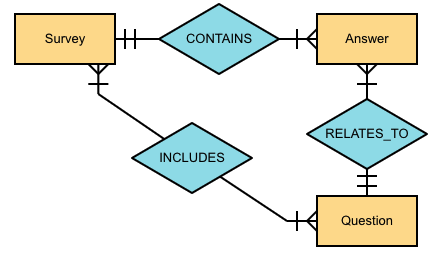
\includegraphics[width=0.45\linewidth]{figures/database/erd-options/Triple.png}\label{fig:triple-relationship}}
    \hfill
    \subfloat[Option 1]{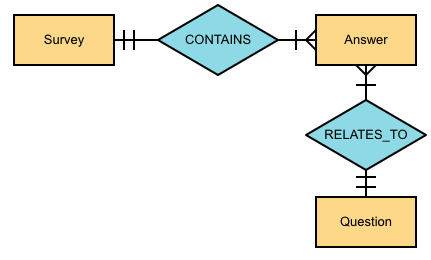
\includegraphics[width=0.45\linewidth]{figures/database/erd-options/Survey-Answer-Question.png}\label{fig:system_1}}
    \hfill
    \subfloat[Option 2]{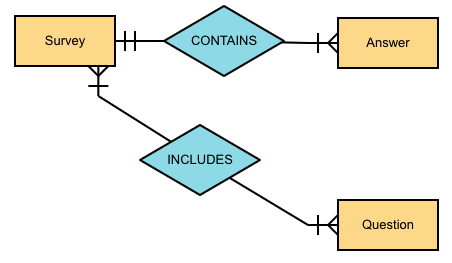
\includegraphics[width=0.45\linewidth]{figures/database/erd-options/Question-Survey-Answer.png}\label{fig:system_2}}
    \hfill
    \subfloat[Option 3]{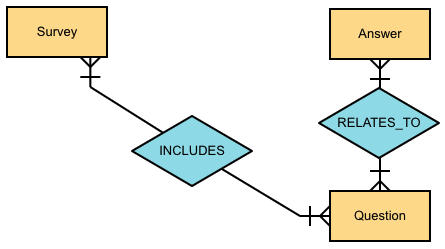
\includegraphics[width=0.45\linewidth]{figures/database/erd-options/Survey-Question-Answer.png}\label{fig:system_3}}
    \caption{Relationship Options}
\end{figure}
\FloatBarrier

\vspace{5mm}

\noindent \textbf{Option 1}: Survey $\rightarrow$ Answer $\rightarrow$ Question [\ref{fig:system_1}] \\
This approach links the Survey directly to the Answer entity, and the Answer is connected to the Question.

\begin{itemize}
    \item \textbf{Advantages}:
    \begin{itemize}
        \item Simpler queries: This design allows us to retrieve answers for a specific survey directly, and then easily map them to the corresponding questions.
        \item Natural data flow: It follows the normal process of a survey, where a user answers questions for a particular survey.
        \item Reduced redundancy: By not connecting Survey directly to Question, we avoid storing duplicate relationships.
    \end{itemize}
    \item \textbf{Disadvantages}:
    \begin{itemize}
        \item Limited flexibility: If you need to make sure each survey is tied to a specific set of questions, it could be harder to manage.
    \end{itemize}
\end{itemize}

\vspace{5mm}

\noindent \textbf{Option 2}: Survey $\rightarrow$ Question, Survey $\rightarrow$ Answer [\ref{fig:system_2}] \\
In this option, the Survey is directly linked to both the Question and Answer entities.

\begin{itemize}
    \item \textbf{Advantages}:
    \begin{itemize}
        \item Manageable survey-question structure: Allows for better control over which questions are included in each survey.
        \item Direct relationship access: Answers and questions are both directly linked to the survey, making it simpler to get either data without needing extra steps.
    \end{itemize}
    \item \textbf{Disadvantages}:
    \begin{itemize}
        \item Additional ``Includes'' table: We need to create an additional table that includes the unique identifiers from both the Survey and Question entities. This table uses the Survey ID and Question ID as combined keys to uniquely identify each instance of the relationship.  The reason for this table is that the relationship between surveys and questions is many-to-many, meaning each survey can contain multiple questions, and each question can appear in multiple surveys.
        \item Redundant connections: Connecting both Survey to Answer and Survey to Question adds extra complexity, especially if the questions are static. These extra links can add unnecessary complexity.
        \item Complicated queries: Retrieving which answers correspond to which questions within a survey becomes more complex and requires additional logic to keep the data accurate.
    \end{itemize}
\end{itemize}

\vspace{5mm}

\noindent \textbf{Option 3}: Survey $\rightarrow$ Question $\rightarrow$ Answer [\ref{fig:system_3}] \\
In this option, the Survey is connected directly to the Question entity, and the Answer is connected to the Question.

\begin{itemize}
    \item \textbf{Advantages}:
    \begin{itemize}
        \item Consistent survey-question associations: Makes it easy to guarantee that surveys only contain the right questions, preventing any mistakes in assigning questions to surveys.
    \end{itemize}
    \item \textbf{Disadvantages}:
    \begin{itemize}
        \item Additional ``Includes'' table: Similar to the structure discussed in Option 2, this approach also requires the creation of an extra table to the database, in order to link Surveys and Questions.
        \item Complex querying: Querying the data becomes more complicated since you’ll need to go through both Survey and Question to get the answers.
        \item Possible duplication: Since the questions are fixed, directly connecting both Survey and Question might introduce unnecessary relationships and add more complexity.
    \end{itemize}
\end{itemize}

\vspace{5mm}

\noindent \textbf{Conclusion} \\
After evaluating all three options, I have decided to go with \textbf{Option 1} (Survey $\rightarrow$ Answer $\rightarrow$ Question [\ref{fig:system_1}]). This approach offers a balance of simplicity and efficiency, making it easier to query data without adding unnecessary complexity. By connecting the Survey directly to the Answer entity, and the Answer to the Question, we maintain a natural flow of data where users respond to questions within the context of a survey. This design reduces the potential for duplicated or unnecessary relationships, as there is no direct link between the Survey and Question entities. While Option 2 and Option 3 provide better control over survey-question relationships, they also require the creation of additional tables and result in more complex queries. Since the questions in the survey are static and do not change, Option 1 offers a cleaner, more efficient and flexible model that suits the application's needs.

\vspace{5mm}

\begin{enumerate}[resume]
    \item \textbf{No connection to Message entity}
\end{enumerate}

\noindent As you may have noticed, I chose not to create a direct relationship between the Message entity and any other entities in the ERD. The reason for this is that the Message entity is exclusively intended to store quotes and advice that are displayed to users, without the need to assign a message to a particular user in the database. I avoided this connection because I don't need to track which user receives which specific message. Instead, the link between users and messages is handled at the backend level, where a user receives a randomly selected message based on their overall mood level. This approach is more general, but keeps the database clean while ensuring dynamic message delivery during runtime.

\subsection{UML}

Having finalized the ERD, the next step involves translating that design into the UML diagram of the database schema and I am going to use \textbf{\href{https://www.dbdesigner.net/}{DBDesigner}}\footnote{Link: \url{https://www.dbdesigner.net/}} to do it. This tool provides a clearer visualization of table configurations, foreign key constraints, and relationships without the need for manual SQL queries. It gives an overview of how the tables interact through primary and foreign keys, making it easier to manage and validate the relationships before proceeding to actual implementation.\vspace{5mm} \\
The UML for the application is shown below:

\vspace{5mm}

\FloatBarrier
\begin{figure}[ht]
    \centering
    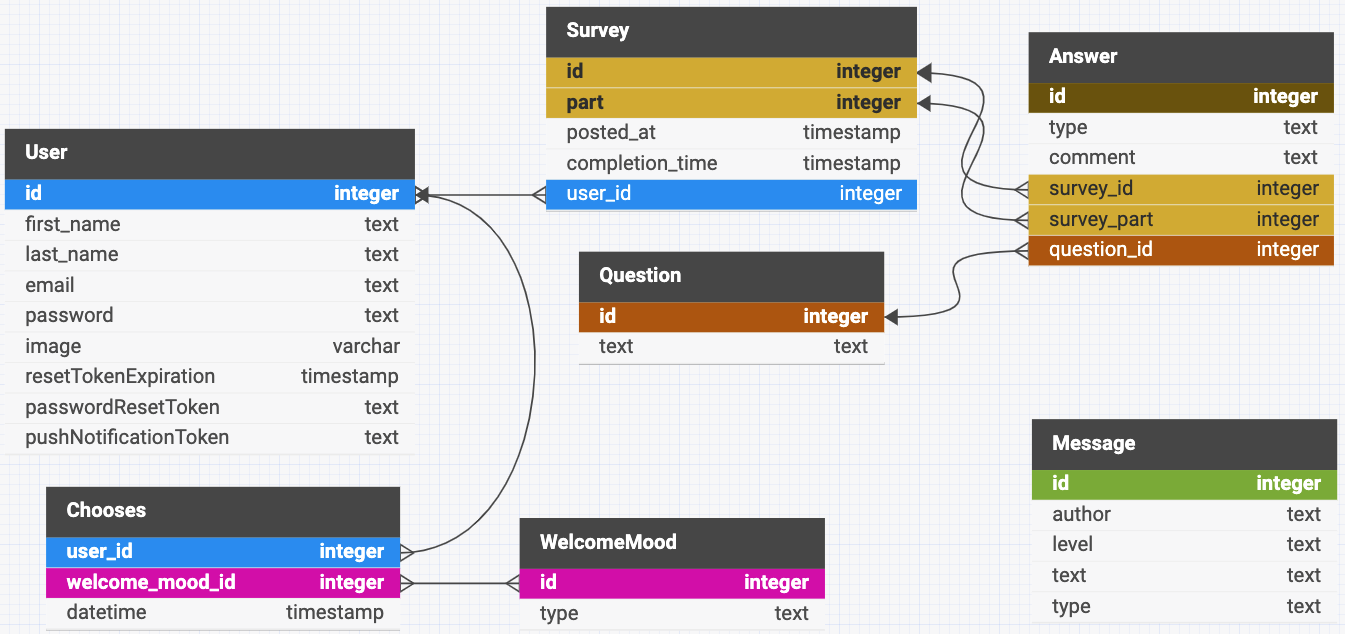
\includegraphics[width=\linewidth]{figures/database/UML.png}
    \label{fig:uml}
    \caption{UML}
\end{figure}
\FloatBarrier

\noindent Each rectangle in the UML diagram represents a separate table in the database, and these tables hold the actual data. Each attribute listed in the rectangle corresponds to a column in the table, with the value types next to each attribute name indicating the data type of that attribute (such as text, integer, or timestamp). The arrows connecting the tables represent relationships between these tables, which were discussed previously in the ERD design phase.\vspace{5mm} \\
For example, I created the table for the \textbf{Survey}, but because of the ``Completes'' relationship between the User and Survey, the Survey table also contains the \textbf{user\_id}. This allows us to track which user completed each survey by using the ``user\_id'' as a foreign key in the Survey table.\vspace{5mm} \\
Another important case is the relationship between User and WelcomeMood, which is a many-to-many relationship. Since databases do not support many-to-many relationships directly, I had to create an additional table called \textbf{Chooses}. This table includes the unique identifiers from both the User and WelcomeMood tables (\textbf{user\_id} and \textbf{welcome\_mood\_id}). The table also contains the attribute \textbf{datetime}, which comes from the relationship itself, capturing when a user chooses a welcome mood.\vspace{5mm} \\
The same logic applies to all the other relationships. For instance, the attribute \textbf{completion\_time} in the \textbf{Survey} table is an attribute that comes from the ``Completes'' relationship. This attribute tracks when a survey was completed by a user and helps maintain historical data regarding user participation.\vspace{5mm} \\
This UML diagram helps visualize the structure of the database, showing how tables are connected through relationships and what attributes each table holds. It’s an essential tool for ensuring that the database schema is correct and efficient before we proceed to the implementation phase.

\section{Database Implementation}
After designing the database schema, the next step is to choose the type of database that best supports the application. I decided to use a \textbf{relational database management system (RDBMS)} instead of a non-relational one (e.g. MongoDB) for several reasons. First, the structure of the application involves clear relationships between entities, such as users completing surveys and submitting answers. These relationships are best handled in a relational database where foreign keys and joins can efficiently manage the connections between tables. Additionally, RDBMS like PostgreSQL ensure strong data consistency, integrity, and support for complex queries, which are essential when managing interconnected datasets, such as survey answers linked to specific questions.\vspace{5mm} \\
Among the various RDBMS options, I chose \textbf{\href{https://www.postgresql.org/}{PostgreSQL}}\footnote{Link: \url{https://www.postgresql.org/}} over others (e.g., MySQL, SQLite, etc.). PostgreSQL is a powerful, open-source relational database management system that offers several advanced features which align perfectly with the needs of this application. One of the key advantages of PostgreSQL is its flexibility and support for advanced data types, making it easier to handle the variety of data formats used in the application. PostgreSQL is also highly reliable because it follows the ACID principles (Atomicity, Consistency, Isolation, Durability)\footnote{The ACID principles are a set of properties that ensure reliable processing of database transactions. \textbf{Atomicity} guarantees that each transaction is all or nothing. \textbf{Consistency} ensures that a transaction can only bring the database from one valid state to another. \textbf{Isolation} maintains that the execution of transactions is independent of one another. \textbf{Durability} assures that once a transaction has been committed, it will remain so, even in the event of a system failure.}. This means that even if the system crashes or something goes wrong, PostgreSQL ensures that the data remains correct and safe. On top of that, PostgreSQL has a large, active community that continuously provides support, updates, and improvements to keep it stable and up-to-date.

\subsection{Xata}
To host and manage the PostgreSQL database, I decided to use \textbf{\href{https://xata.io/}{Xata}}\footnote{Link: \url{https://xata.io/}}, a fully managed cloud database platform for PostgreSQL. Xata makes it easy to handle the database by automatically taking care of things like scaling, backups, and monitoring, so I can focus more on developing the application rather than worrying about database maintenance.
\begin{itemize}
    \item \textbf{PostgreSQL Compatibility}: Xata uses PostgreSQL as its underlying engine, meaning it inherits all of PostgreSQL’s strengths while adding a layer of simplicity and automation.
    \item \textbf{User-Friendly Interface}: One of Xata's key advantages is that it allows you to create and manage the database without writing any queries. The platform provides an intuitive and easy-to-use interface, making it simple to set up, modify, and maintain the database without requiring deep technical expertise. This ease of use greatly simplifies the process, especially for rapid development and iteration.
    \item \textbf{NoOps Framework}: Xata offers a ``NoOps'' solution, meaning that there is no need for manual intervention for scaling, backups, or maintenance. This greatly reduces operational overhead and ensures that the database performs efficiently as the application scales.
    \item \textbf{Cloud-Native and Fully Managed}: Xata allows easy scaling, automated backups, and real-time monitoring. As the application grows and more users engage with the platform, the database automatically adjusts without the need for manual scaling.
\end{itemize}

\noindent Compared to traditional platforms like AWS RDS, Xata provides a more developer-friendly interface, easier integration, and reduced operational complexity, making it ideal for projects that need to iterate and scale quickly, such as this application. However, one drawback of Xata is that when saving data through a localhost server, it records the time information three hours earlier than expected. This inconsistency disrupts functionalities like scheduling random survey times between 12:00 and 20:00, tracking user survey completion times, and executing time-sensitive tasks like notifications, impacting the application's intended workflow.

\subsection{Database Schema}
I created the database schema in the Xata platform, but first, we need to explain some features that the platform provides.\vspace{5mm} \\
When creating a table in Xata, four essential attributes are automatically generated for every table:

\begin{itemize}
    \item \textbf{id}: This is a unique identifier for each record in the table. It is auto-generated and also has data type ``text''.
    \item \textbf{xata.createdAt}: This attribute captures the exact timestamp when a record is first created in the database. It provides a clear indication of when data was added.
    \item \textbf{xata.updatedAt}: Similar to createdAt, this attribute records the timestamp for when a record was last updated. It is automatically updated whenever any changes are made to the data.
    \item \textbf{xata.version}: This integer field tracks the version of the record. Every time a record is updated, the version increments, allowing for a history of changes and potential conflict resolution.
\end{itemize}

\noindent The only attribute we’ll rely on during the implementation phase is the id. The others—createdAt, updatedAt, and version—serve as metadata for manual data management.\vspace{5mm} \\
Furthermore, the small rectangles on the left side of the attributes, these symbols indicate the required status of the field:
\begin{itemize}
    \item \textbf{Solid Diamond}: This signifies that the attribute is mandatory, meaning it cannot be null or empty.
    \item \textbf{Empty Diamond}: This denotes an optional attribute, meaning it can be left blank or null.
\end{itemize}

\noindent Additionally, the ``handprint'' icons next to certain attributes indicate that these columns have a unique constraint. This means that the values in these fields must be unique across all records in the table. For example, the id column typically has this icon, as it is the primary unique identifier for each record in the table. This constraint ensures that no two records can have the same value for that attribute, which is critical for maintaining data unity.\vspace{5mm} \\
We defined all the information that we need for undestanding the xata database schema, so we can proceed to the designing of it. The final schema is shown below:

\FloatBarrier
\begin{figure}[ht]
    \centering
    \subfloat[User]{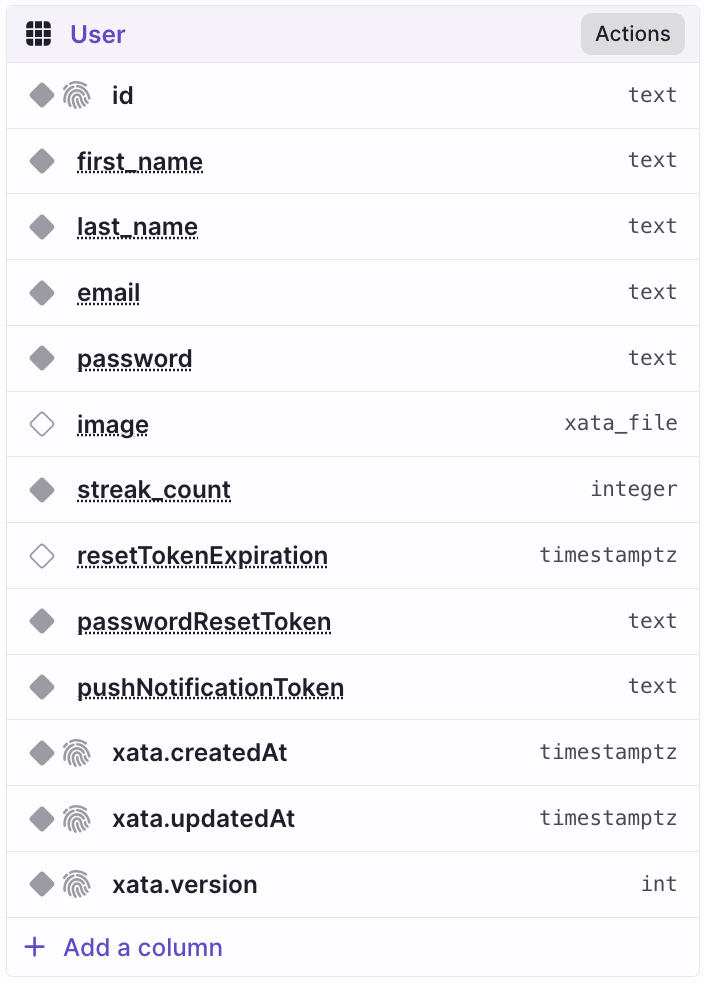
\includegraphics[width=0.49\linewidth]{figures/database/schema/User.png}\label{fig:user}}
    \hfill
    \subfloat[Survey]{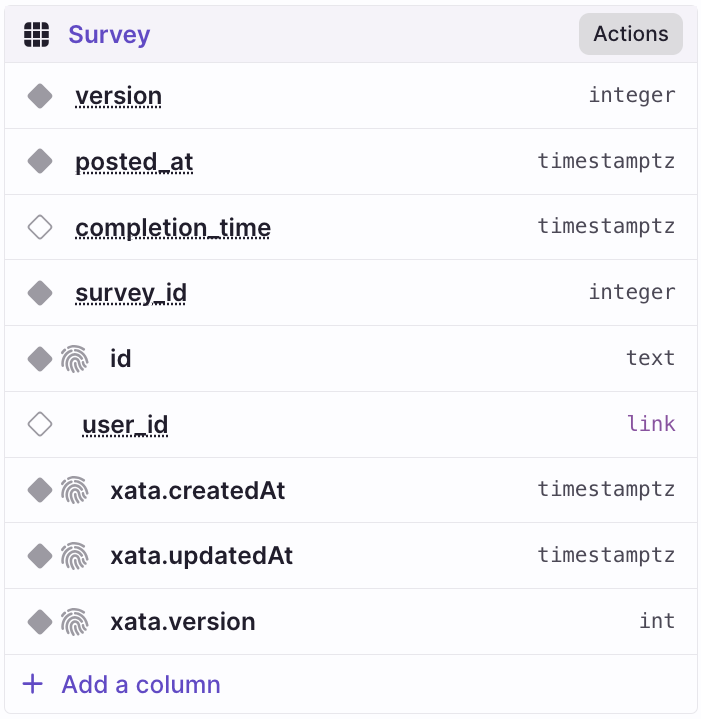
\includegraphics[width=0.49\linewidth]{figures/database/schema/Survey.png}\label{fig:survey}}
\end{figure}
\FloatBarrier

\FloatBarrier
\begin{figure}[ht]\ContinuedFloat
    \centering
    \subfloat[Message]{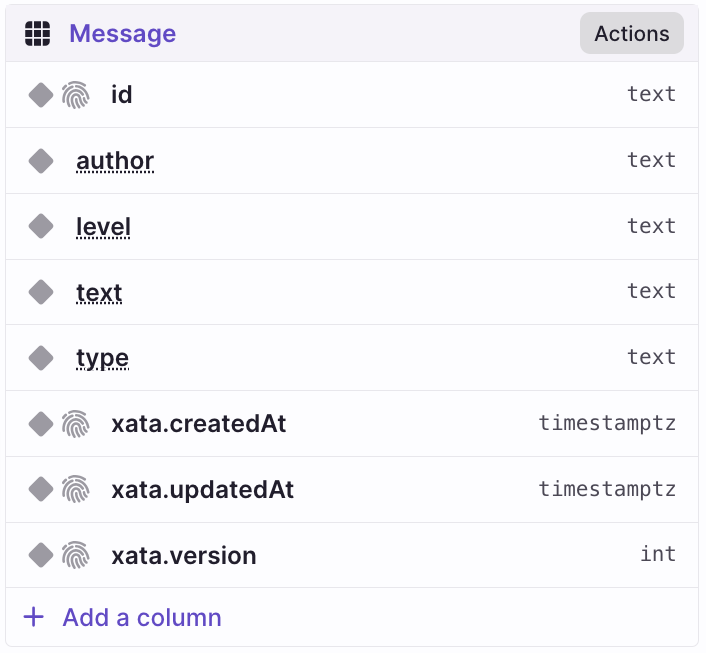
\includegraphics[width=0.49\linewidth]{figures/database/schema/Message.png}\label{fig:message}}
    \hfill
    \subfloat[Answer]{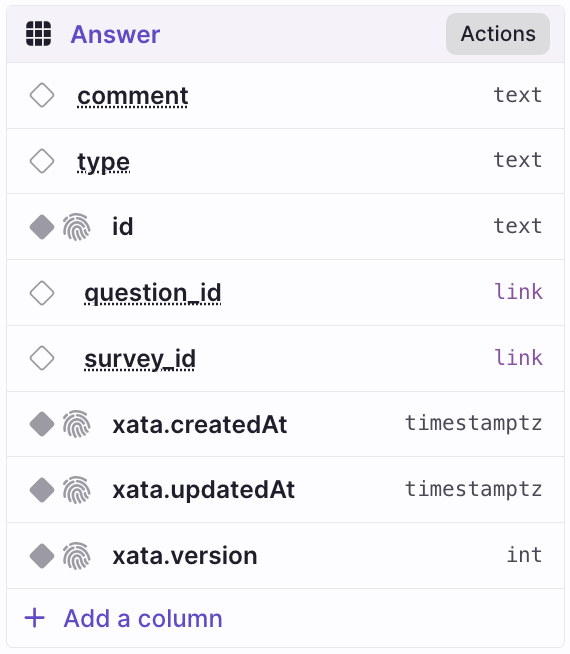
\includegraphics[width=0.49\linewidth]{figures/database/schema/Answer.png}\label{fig:answer}}
\end{figure}
\FloatBarrier

\FloatBarrier
\begin{figure}[ht]\ContinuedFloat
    \centering
    \subfloat[Chooses]{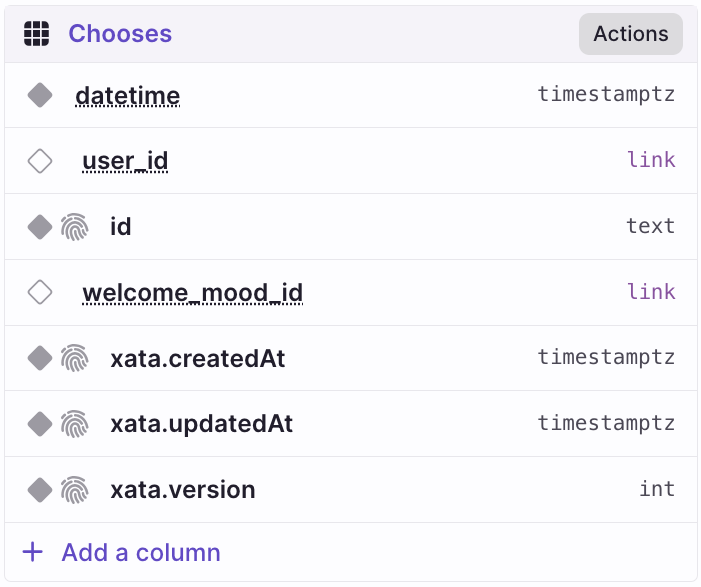
\includegraphics[width=0.49\linewidth]{figures/database/schema/Chooses.png}\label{fig:chooses}}
    \hfill
    \subfloat[Question]{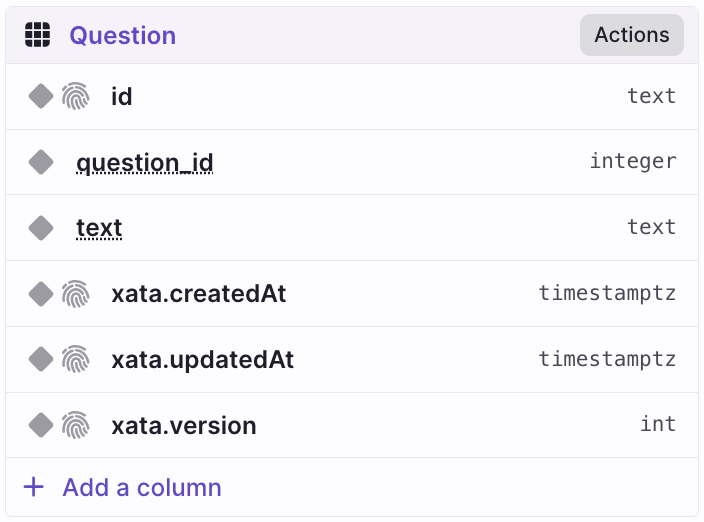
\includegraphics[width=0.49\linewidth]{figures/database/schema/Question.png}\label{fig:question}}
\end{figure}
\FloatBarrier

\FloatBarrier
\begin{figure}[ht]\ContinuedFloat
    \centering
    \subfloat[Welcome Mood]{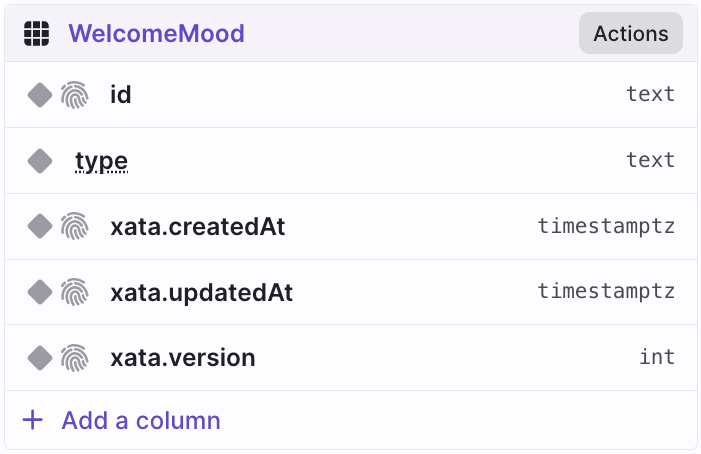
\includegraphics[width=0.6\linewidth]{figures/database/schema/WelcomeMood.png}\label{fig:welcome_mood}}
    \caption{Database Schema}
\end{figure}
\FloatBarrier

\vspace{5mm}

\noindent As we transition from UML diagrams to the actual database schema, some fields that were not assigned an ID in the UML, now have one in the Xata database. Xata automatically generates IDs with a text data type, which led us to modify certain fields to better align with our database structure:

\begin{enumerate}
    \item The ``id'' of the \textbf{User} table changes its data type from integer to text.
    \item The ``id'' of the \textbf{Survey} table is named ``survey\_id'', retaining its integer data type to facilitate future queries and functionality. As a result, the updated \textbf{Survey} table includes:
    \begin{itemize}
        \item A Xata auto-generated \textbf{id} with a text data type, serving as the unique identifier.
        \item A \textbf{survey\_id} with an integer data type, representing the original ``id'' from the UML.
        \item The \textbf{version} attribute, renamed from the previous ``part'' attribute.
    \end{itemize}
    \item The \textbf{Answer} table references only ``survey\_id'' as its foreign key, following the update to the ``id'' in the \textbf{Survey} table. The ``id'' data type is changed from integer to text.
    \item The ``id'' of the \textbf{Question} table becomes ``question\_id'', keeping its integer data type for easier querying and functionality. Consequently, the \textbf{Question} table includes:
    \begin{itemize}
        \item A Xata auto-generated \textbf{id} with a text data type as the unique identifier.
        \item A \textbf{question\_id} with an integer data type, corresponding to the original ``id'' in the UML.
        \item The \textbf{text} attribute, which remains unchanged from the UML.
    \end{itemize}
    \item The \textbf{Chooses} table receives a new auto-generated ``id'' with a text data type as its unique identifier.
    \item The \textbf{WelcomeMood} table changes the data type of its ``id'' from integer to text.
    \item The \textbf{Message} table also changes the data type of its ``id'' from integer to text.
\end{enumerate}

\noindent In summary, every table designed in the UML has a corresponding table in the Xata database with the same name and data type, and in addition, they all get these automatically generated fields (id, createdAt, updatedAt, version) to manage their records more efficiently.

\section{Project Setup}

To begin developing the application, the first step is to create a repository on \textbf{\href{https://github.com/}{GitHub}}\footnote{Link: \url{https://github.com/}}. GitHub is an essential tool for hosting, managing, and version-controlling code, allowing easy collaboration and tracking of changes. By using GitHub, I can maintain a clear history of my project's progress. Additionally, GitHub ensures that all stages of development, from initial research and design to implementation, are captured and safely stored. I have already created a repository named \textbf{Mood\_Tracker}, which served as a central location to track and document every major step prior to implementation, such as research, design, and planning.\vspace{5mm} \\
Next, I organized the project into two main directories:

\begin{itemize}
    \item \textbf{frontend}: This folder contains everything related to the user interface (UI) and front-end development of the application. All components that handle user interaction, design, and rendering is contained here.
    \item \textbf{api}: This folder manages the back-end development and API services. It includes code that handles data storage, processing, and communication between the frontend and server.
\end{itemize}

\noindent For each of the folders, I initialize them using \textbf{\href{https://www.npmjs.com/}{npm (Node Package Manager)}}\footnote{Link: \url{https://www.npmjs.com/}}. NPM is a critical tool for managing JavaScript dependencies and automating the setup of a project. By running ``npm init'' and providing the necessary information about each project folder, I generate the necessary configuration files for managing third-party packages and development scripts for each of folder, which is important as the project grows. It helps streamline the process of installing and updating the libraries that the project may require.\vspace{5mm} \\
With this basic structure in place, I proceed with developing the frontend, focusing first on creating the user interface for tracking moods and interacting with the application.

\section{Front-end Development}
Before diving into the folder structure of the front-end, it’s essential to mention that \textbf{\href{https://reactnative.dev/}{React Native}}\footnote{Link: \url{https://reactnative.dev/}} is the perfect framework for building our cross-platform application. React Native allows developers to use a single codebase to create apps for both iOS and Android, providing a cost-effective and time-efficient solution without compromising on performance. It uses native components and JavaScript to create a seamless, native-like user experience across platforms.\vspace{5mm} \\
To simplify development with React Native, we are making use of \textbf{\href{https://expo.dev/}{Expo}}\footnote{Link: \url{https://expo.dev/}}.

\subsection{Expo Setup and Visualization}
Expo is a powerful tool designed to simplify the development and testing of React Native applications. It enables developers to quickly test their apps on real devices or simulators and offers features such as hot reloading, instant builds, and easy deployment. Using Expo allows us to rapidly iterate and visualize our application as we build it.\vspace{5mm}

\noindent \textbf{Project Setup with Expo} \\
\noindent To set up the project with Expo, we follow these steps:

\begin{enumerate}
    \item \textbf{Install Expo CLI}: We begin by installing the Expo command-line interface (CLI) globally using npm:
    \begin{verbatim} npm install -g expo-cli \end{verbatim}
    \item \textbf{Initialize the Project}: Once the CLI is installed, create a new Expo project by running the following command:
    \begin{verbatim} expo init frontend \end{verbatim}
    This command initializes a new project with a basic folder and file structure necessary for Expo and React Native development.
    \item \textbf{Run the Project}: After initializing the project, we navigate into the project folder and start the development server using:
    \begin{verbatim} expo start \end{verbatim}
    This opens the Expo Dev Tools in our browser, providing options to run the app on a simulator, an emulator, or a physical device via QR code.
\end{enumerate}

\vspace{5mm}

\noindent \textbf{Files and Folders Created by Expo} \\
The folder structure that is being automatically generated by Expo is the following:

\vspace{5mm}

\begin{lstlisting}[caption=Expo Project Folder Structure]
. (root folder)
|-- App.js
|-- app.json
|-- assets
    |-- icon.png
    |-- splash.png
|-- babel.config.js
|-- node_modules/
|-- package.json
|-- .gitignore
|-- eas.json
\end{lstlisting}

\vspace{5mm}

\noindent Now, let's break down and explain the purpose of each file and folder in this structure:

\begin{itemize}
    \item \textbf{App.js}: The main entry point of the application. This file contains the root React component that Expo loads and displays when the app is launched.

    \item \textbf{app.json}: This configuration file contains metadata about the app, such as its name, version, and icon settings. It also holds configuration data used by Expo for managing the app build and deployment processes.

    \item \textbf{assets/}: This folder holds static resources like images, fonts, and other media files.
    
    \item \textbf{icon.png}: A default icon for the app.

    \item \textbf{splash.png}: A default splash screen image that is displayed while the app is loading.

    \item \textbf{babel.config.js}: A configuration file for Babel, the JavaScript compiler. This file ensures that modern JavaScript code can be converted into a format compatible with older environments.

    \item \textbf{node\_modules/}: This folder contains all of the npm dependencies required for the project, including React Native, Expo SDK, and any third-party libraries.

    \item \textbf{package.json}: This is the core configuration file that lists the project's dependencies, scripts, and metadata. It ensures that the correct versions of the necessary libraries are installed and used.

    \item \textbf{.gitignore}: A file that specifies which files and folders should be ignored by Git. It typically includes entries such as `node\_modules/` and other files that should not be tracked by version control.

    \item \textbf{eas.json}: This file is part of Expo Application Services (EAS) and configures options for building, submitting, and updating the application using Expo's cloud services.
\end{itemize}

\subsection{Folder Structure of the Front-end}

Having initialized the project using Expo, we define the structure of the frontend folder. Below is the complete folder structure that outlines the key components of the front-end development environment:

\vspace{5mm}

\begin{lstlisting}[caption=frontend Folder Structure]
. (frontend - root folder)
|-- App.js
|-- Dockerfile
|-- app
    |-- assets
        |-- app-images
        |-- fonts
        |-- images
        |-- lottie-animations
        |-- message-images
    |-- components
    |-- config
    |-- constants
    |-- context
    |-- controllers
    |-- navigators
    |-- screens
        |-- Layout.jsx
        |-- extras
        |-- main
        |-- password
        |-- start
        |-- stats
        |-- survey
    |-- services
    |-- utilities
|-- .env
|-- app.json
|-- babel.config.js
|-- eas.json
|-- eslint.config.mjs
|-- jsconfig.json
|-- metro.config.js
|-- package-lock.json
|-- package.json
|-- react-native.config.js
\end{lstlisting}

\vspace{5mm}

\noindent I didn't use a specific architecture pattern for the React Native project. Instead, I focused on implementing best practices and drew inspiration from folder structures commonly adopted by experienced developers in the react native community. This approach allowed me to keep the project structure organized and scalable without being tied to a strict architectural convention.\vspace{5mm} \\
One of the main goals when organizing the code into folders like \textbf{components}, \textbf{screens}, \textbf{services} and \textbf{controllers} was to ensure a clear separation of concerns\footnote{The principle of separation of concerns advocates dividing a program into distinct sections, where each section addresses a specific concern or responsibility. This improves code maintainability and scalability.}. This structure makes it easy to locate and manage different parts of the codebase, providing reusability and maintainability. Grouping related functionalities into their respective folders (e.g., UI elements in components, business logic in controllers, and reusable functions in utilities) helps to reduce complexity and improves the readability of the code. Additionally, the flexibility of this structure allows for easier testing and future scaling of the project.

\subsection{Root-Level Files}
In this section, we provide detailed descriptions of the root-level files that were not covered during the Expo initialization. These files play a critical role in configuring, managing, and building the application.

\begin{itemize}
    \item \textbf{.env}: Holds all the necessary information for the application to properly function, like keys, urls, passwords etc.

    \item \textbf{Dockerfile}: Contains instructions to build a Docker image for the project. Docker ensures that the app can run consistently across different environments by containerizing the application.

    \item \textbf{eslint.config.mjs}: ESLint is a tool for identifying and fixing code quality issues. This file contains the configuration settings for the ESLint linter, which ensures that the code adheres to best practices and consistent formatting.

    \item \textbf{jsconfig.json}: This file provides configuration for JavaScript language features in IDEs, such as Visual Studio Code. It helps with intelligent code completion, module resolution, and path aliasing, making development smoother and more efficient.
    
    \item \textbf{metro.config.js}: This configuration file is for Metro, the JavaScript bundler used in React Native projects. It defines how assets, modules, and dependencies are processed and bundled for the application.

    \item \textbf{package-lock.json}: This file locks the versions of npm dependencies installed in the project, ensuring consistency across different environments. It guarantees that the same versions of libraries are used whenever the project is installed.

    \item \textbf{react-native.config.js}: This file contains specific configuration options for React Native, such as linking native dependencies or customizing how the React Native CLI handles assets and modules.
\end{itemize}

\subsection{app folder}
This is the core directory of the front-end application that organizes the main components, configurations, assets, and services. The app folder structure is the following:

\vspace{5mm}

\begin{lstlisting}[caption=app Folder Structure]
. (app - root folder)
|-- assets
|-- components
|-- config
|-- constants
|-- context
|-- controllers
|-- navigators
|-- screens
|-- services
|-- utilities
\end{lstlisting}

\vspace{5mm}

\begin{itemize}
    \item \textbf{assets/}: Contains all the static resources required by the app, such as images, fonts, and animations.
    \begin{itemize}
        \item \textbf{app-images/}: Stores images used within the app, such as icons, logos, or other custom images that are displayed in the UI.
        \item \textbf{fonts/}: Contains custom fonts that are used throughout the app to ensure a constant visual style.
        \item \textbf{images/}: Holds additional images that are used for UI elements, such as backgrounds or illustrations.
        \item \textbf{lottie-animations/}: A folder dedicated to storing Lottie animation files in JSON format, used for adding lightweight, scalable animations to the app.
        \item \textbf{message-images/}: Contains images used in the ``Message'' components, to provide a more appealing background image to the quote or advice.
    \end{itemize}

    \item \textbf{components/}: This folder contains reusable UI components such as buttons, input fields, modals, and other interface elements. These components are designed to be modular and reusable across various screens. I explain below the purpose of each component:

    \begin{itemize}
        \item \textbf{SurveyButtons.jsx}: Provides buttons used within the `SurveyQuestion' screen, including ``Continue'', ``Exit'', and ``Submit''.
        
        \item \textbf{AnswerSelector.jsx}: A component used within the `SurveyQuestion` screen. It displays the three answer options that the user can select from. The component is rendered three times in a row, once for each answer option.

        \item \textbf{DailyMood.jsx}: Represents the mood for a specific day and is used within the `WeeklyStats` component to visually display the mood data for each day of the week.
        
        \item \textbf{WeeklyStats.jsx}: Uses multiple `DailyMood` components to show the user's mood for each day of the past week. It is displayed on the `Home' screen to give a quick summary of the user’s weekly mood history.
        
        \item \textbf{CalendarOptions.jsx}: Shows options for filtering moods displayed in the `MoodCalendar` component. It allows users to view the occurrence of each specific mood (e.g., nothing, happy, sad) on the calendar. Users can click on any of the six mood options to filter the calendar view accordingly.
        
        \item \textbf{MoodCalendar.jsx}: The main calendar component used in the `Calendar' screen. It visually represents the welcome moods the user has logged, arranged in a calendar format. The `CalendarOptions` component works with `MoodCalendar` to filter and display specific moods.
        
        \item \textbf{Emoji.jsx}: A child component used within `EmojiSelector` that displays a single emoji icon, along with animations and color changes. It visually represents different mood options using emojis.
        
        \item \textbf{EmojiSelector.jsx}: Used on the `Welcome' screen for selecting an emoji that represents the user’s mood. It includes multiple `Emoji` components, each allowing the user to choose how they feel at the moment.
        
        \item \textbf{EmotionLegend.jsx}: Provides a legend explaining the meaning of each mood and its corresponding color or icon. This component is displayed twice throughout the app, ensuring users understand the visual representation of moods.
        
        \item \textbf{HeaderAvatar.jsx}: Displays the user’s profile avatar in the top-right corner of the header projected in the `Home' and `Questionnaires' screens. It is implemented within the `MainNavigator` to keep it consistent across these screens.
        
        \item \textbf{HeaderTitle.jsx}: Displays the user’s name along with a welcome message and the current survey streak. It also indicates if the daily survey has been completed. Like `HeaderAvatar`, this component is also part of the `MainNavigator` header implementation, to maintain a consistent header design.
        
        \item \textbf{Message.jsx}: Shows quotes or advice on the `Home' screen, providing daily inspiration to the user.
        
        \item \textbf{MyModal.jsx}: Displays a modal with a loading state, preventing user interaction during certain operations. It is mainly used on the `Profile' screen when updating the user’s image.
        
        \item \textbf{GoBackButton.jsx}: A reusable button component with an arrow icon pointing to the left. It is used throughout the app for navigation, making it easy for users to go back to the previous screen.
        
        \item \textbf{SideButton.jsx}: Used in the `Profile' screen to provide options related to the user’s avatar image, such as editing or deleting the profile picture. They are being triggered when the user presses on the avatar image.
        
        \item \textbf{LabelInput.jsx}: Used for the input fields on the `Profile' screen, allowing users to see and edit their personal information.
        
        \item \textbf{InformationLabel.jsx}: Displays screen labels on top of each statistic screens, such as “All Welcome Moods” on the `Calendar' screen and “All Questionnaires” on the `Graph' screen, to give context about the data shown.
        
        \item \textbf{PreviousSurvey.jsx}: Displays information about each previous survey completed by the user, shown on the `Questionnaires' screen.
        
        \item \textbf{Button.jsx}: A general-purpose, reusable button component used throughout the app. It provides consistent styling and easy configuration for various button types and actions.
        
        \item \textbf{MoodBarChart.jsx}: Displays a bar chart visualization of the user’s questionnaires' scores on the `Graph' screen, providing a visual representation of their responses over time.
        
        \item \textbf{MoodPieChart.jsx}: Shown below `MoodBarChart` on the `Graph' screen, this component presents a pie chart that divides the survey data into five mood categories (awful, sad, neutral, good, happy) for a more detailed analysis.
        
        \item \textbf{MonthlyStats.jsx}: Projects a condensed version of the user’s questionnaire responses over the past month. It is displayed on the `Home' screen, providing a snapshot of recent survey results.
    \end{itemize}
        

    \item \textbf{config/}: Contains configuration files for different parts of the application. This folder includes specific files such as configuration for animations (animationConfig.js), custom component bordering (borderConfig.js), custom text colors for the ``Message'' component (messageConfig.js), different moods and respective colors (moodConfig.js), and shadows (shadowConfig.js). Keeping configurations in a centralized folder allows for easy management and updates.

    \item \textbf{constants/}: This folder stores constant values used throughout the app, such as color codes, dimensions, fonts.

    \item \textbf{context/}: Contains React context files that manage global state across the application. The Context API is used to handle processes such as user authentication (AuthContext.js), managing daily survey data (DailySurveyContext.js), tracking welcome mood completion (MoodContext.js), and handling user information in the ``Profile'' screen (ProfileContext.js). These contexts ensure that important data is easily accessible across multiple components and screens.

    \item \textbf{controllers/}: This folder houses the business logic of the app, such as functions that handle user input and data processing. Controllers primarily serve as a bridge between UI components and service functions. They do not make API requests directly, but instead, they call the functions from the services folder, which handles all communication with the backend. For example, appController.js handles logic related to the App.js file, while homeController.js is responsible for the logic in the Home screen. This separation ensures that complex operations are managed within controllers, keeping the UI components clean and focused on rendering, and delegating all API interactions to the corresponding services files. This division of responsibilities helps maintain a clear and organized structure, making the code easier to understand and maintain.

    \item \textbf{navigators/}: This folder manages the navigation structure of the app using React Navigation. It contains files that define how users move between different screens, organizing the app's navigation logic into various navigators for different sections of the app. Each file corresponds to a specific type of navigation or part of the application:
    
    \begin{itemize}
        \item \textbf{BottomNavigator.jsx}: Manages bottom tab navigation, allowing users to switch between different sections of the app using a bottom navigation bar.
        \item \textbf{MainNavigator.jsx}: The primary navigator for the app, coordinating the overall flow between major screens and managing top-level navigation.
        \item \textbf{StartNavigator.jsx}: Handles the navigation for the onboarding process, including screens for sign-in, sign-up, and welcome flows and also the ``Main Navigator''.
        \item \textbf{StatsNavigator.jsx}: Manages the navigation between screens related to user statistics, such as `Calendar' and `Graph'.
        \item \textbf{SurveyNavigator.jsx}: This file is responsible for navigating through the survey screens, managing the flow from one survey question to the next.
    \end{itemize}

    \noindent This structure keeps the navigation logic organized by app sections, making it easier to maintain and understand.

    \item \textbf{screens/}: Contains all the individual screens that users interact with in the app. Each screen represents a page or view in the app, such as the home screen, profile screen and others.
    \begin{itemize}
        \item \textbf{Layout.jsx}: This file defines the layout structure of the app, managing how different screens are arranged and rendered. Basically it is used to apply header space for the header of the application, or a footer space (optional) for adding the bottom navigation bar to each screen.
        \item \textbf{extras/}: Contains additional screens that handle special cases using Lottie animations, such as loading screens or error pages. These files include:
        \begin{itemize}
            \item AppLoading.jsx: Manages the loading screen shown when the survey data is being fetched.
            \item Completion.jsx: Appears after a user completes a survey.
            \item Connecting.jsx: Used to show a connection status screen after the user connects to the application.
            \item NoSurvey404.jsx: Displays a ``404 - Google Dinosaur Game'' style error page when no survey is found.
            \item Splashscreen.jsx: Manages the initial splash screen shown when the app starts.
        \end{itemize}

        \noindent Each of these components ensures a smooth user experience during specific states or transitions within the app.

        \item \textbf{main/}: Holds the core screens of the application, such as the ``Home'' screen, ``Profile'' screen and the ``Questionnaires'' screen.
        \item \textbf{password/}: Contains screens related to password management, such as ``Request Password Reset'' and ``Password Reset'' screens.
        \item \textbf{start/}: Contains onboarding-related screens, such as ``Sign-in'', ``Sign-up'', and ``Welcome'' screens that users interact with when they first use the app.
        \item \textbf{stats/}: Contains screens for displaying statistics, such as the ``Calendar'' and the ``Graph'' screen.
        \item \textbf{survey/}: Contains the ``SurveyQuestion'' screen that is responsible for managing the survey process. ``SurveyQuestion'' represents the screen for one question at a time.
    \end{itemize}

    \item \textbf{services/}: Contains functions that interact with external services or APIs, handling tasks such as authentication, data fetching, and communication between the front-end and back-end systems. Each file is paired with a corresponding backend route file of the same name, ensuring seamless communication and data exchange between the client and server.

    \item \textbf{utilities/}: Contains utility functions used throughout the app. These include helper functions for handling date and time operations, encoding and decoding with hashing, selecting images (pickImage function), calculating mood counts for a given month, and a ratio function that assigns specific colors or emotions based on numeric values. These utilities streamline common tasks and keep the codebase organized by separating frequently reused logic.
\end{itemize}

\noindent Before diving into the details of the Authorization Process, it’s worth highlighting that this functionality is the most complicated part of the front-end implementation. Unlike most other front-end controller or context functions, which primarily involve data fetching, processing, and displaying, the authorization process encompasses complex logic for managing user sessions, maintaining data privacy, and ensuring secure communication between the client and server.

\subsection{Authorization Process}

The authorization process in the application is responsible for managing user authentication, including signing up, signing in, and signing out. It also handles persisting session data, allowing users to remain logged in across app sessions. Below is a breakdown of the key functions involved in this process:

\begin{enumerate}
    \item \textbf{signUp (Sign-Up Process)}
    \begin{itemize}
        \item This function is responsible for registering a new user. \item It first calls registerForPushNotificationsAsync to obtain a push notification token, ensuring the user can receive notifications.
        \item Once the token is obtained, it calls the handleSignUp service to create a new account in the backend, passing the user’s details and the notification token.
        \item Upon successful registration, it stores the returned authentication data (authData) and token in AsyncStorage, allowing the app to recognize the user during future sessions.
        \item The connecting state is set to true while the sign-up process is underway, ensuring the user sees feedback during this process.
    \end{itemize}
\end{enumerate}

\begin{lstlisting}[caption={Sign Up Function}]
const signUp = async (firstName, lastName, email, password) => {
    try {
    const pushNotificationToken = await registerForPushNotificationsAsync();
    if (pushNotificationToken) {
        const result = await handleSignUp({
        firstName,
        lastName,
        email,
        password,
        pushNotificationToken,
        });
        setConnecting(true);
        if (result.success) {
        setAuthData(result.data);
        await AsyncStorage.setItem('@AuthData', JSON.stringify(result.data));
        await AsyncStorage.setItem('@AuthToken', result.data.authToken);
        } else {
        throw new Error(result.message);
        }
    } else {
        throw new Error(result.message);
    }
    } catch (error) {
    throw error;
    } finally {
    setTimeout(() => {
        setConnecting(false);
    }, 4000);
    }
};
\end{lstlisting}

\begin{enumerate}[resume]
    \item \textbf{registerForPushNotificationsAsync (Push Notification Registration)}
    \begin{itemize}
        \item This function registers the user’s device for push notifications.
        \item It first checks if the device supports push notifications, and then requests permissions from the user.
        \item If the permission is granted, it retrieves the push notification token via Expo's `getExpoPushTokenAsync` method.
        \item This token is later stored in the backend for sending push notifications to the user.
    \end{itemize}
\end{enumerate}

\begin{lstlisting}[caption={Register Push Notification function}]
// Function to register for push notifications and get the token
const registerForPushNotificationsAsync = async () => {
    let token;
    if (Device.isDevice) {
    const { status: existingStatus } = await Notifications.getPermissionsAsync();
    let finalStatus = existingStatus;
    if (existingStatus !== 'granted') {
        const { status } = await Notifications.requestPermissionsAsync();
        finalStatus = status;
    }
    if (finalStatus !== 'granted') {
        alert('Failed to get push token for push notification!');
        return;
    }
    // Get the Expo push token
    token = (
        await Notifications.getExpoPushTokenAsync({
        projectId: Constants.expoConfig.extra.eas.projectId,
        })
    ).data;
    } else {
    alert('Must use a physical device for Push Notifications');
    }
    return token;
};
\end{lstlisting}
  

\begin{enumerate}[resume]
    \item \textbf{signIn (Sign-In Process)}
    \begin{itemize}
        \item This function is responsible for logging in an existing user.
        \item It calls the `handleSignIn` service with the user’s email and password.
        \item If the authentication is successful, the `authData` returned from the backend is stored in `AsyncStorage` along with the authentication token, allowing the user to remain signed in.
        \item Similar to the sign-up process, the `connecting` state is set to true during the sign-in operation, providing visual feedback while the process is ongoing.
    \end{itemize}
\end{enumerate}

\begin{lstlisting}[caption={Sign In Function}]
const signIn = async (email, password) => {
    try {
    const result = await handleSignIn(email, password);
    if (result && result.data) {
        setAuthData(result.data);
        await AsyncStorage.setItem('@AuthData', JSON.stringify(result.data));
        await AsyncStorage.setItem('@AuthToken', result.data.authToken);
        setConnecting(true);
    } else {
        throw new Error('No auth data returned from sign in');
    }
    } catch (error) {
    throw error;
    } finally {
    setTimeout(() => {
        setConnecting(false);
    }, 4000);
    }
};
\end{lstlisting}

\begin{enumerate}[resume]
    \item \textbf{loadSession (Session Restoration)}
    \begin{itemize}
        \item This function is used to restore the user’s session when the app is opened.
        \item It checks `AsyncStorage` for any previously stored authentication data (`@AuthData`) and loads it into the app’s state if it exists.
        \item This ensures that the user remains logged in across multiple sessions without having to sign in every time the app is opened.
        \item The `loading` state is set to false once the session data is loaded, allowing the app to display the appropriate screen based on the authentication state.
    \end{itemize}
\end{enumerate}

\begin{lstlisting}[caption={Load Session}]
const loadSession = async () => {
    try {
    const authDataSerialized = await AsyncStorage.getItem('@AuthData');
    if (authDataSerialized) {
        const _authData = JSON.parse(authDataSerialized);
        setAuthData(_authData);
    }
    } catch (error) {
    console.error('Failed to load session:', error);
    } finally {
    setLoading(false);
    }
};

// Effect to load session data on app load
useEffect(() => {
    loadSession();
}, []);
\end{lstlisting}

\begin{enumerate}[resume]
    \item \textbf{signOut (Sign-Out Process)}
    \begin{itemize}
        \item This function is responsible for signing the user out of the application.
        \item It clears the authentication data (`@AuthData`) and token (`@AuthToken`) from `AsyncStorage`, effectively logging the user out.
        \item After signing out, the `authData` state is set to `null`, and the user is redirected to the appropriate screen (``Sign In'' Screen).
    \end{itemize}
\end{enumerate}

\begin{lstlisting}[caption={Sign Out Function}]
const signOut = async () => {
    try {
    setAuthData(null);
    await AsyncStorage.multiRemove(['@AuthData', '@AuthToken']);
    } catch (error) {
    console.error('Failed to sign out:', error);
    }
};

if (connecting) return <Connecting />;
\end{lstlisting}   

\begin{enumerate}[resume]
    \item \textbf{Returned Items and Context Value} \\
    The `AuthContext.Provider` returns several key items that manage the app's authorization state:
    \begin{itemize}
        \item \textbf{authData}: Stores the authenticated user’s data, such as their ID, token, and profile information.
        \item \textbf{setAuthData}: A function to manually update the authentication data in the context.
        \item \textbf{loading}: Indicates whether the app is still loading session data, helping manage the display of loading screens.
        \item \textbf{loadSession}: A function that reloads session data from `AsyncStorage` to keep the user signed in across app restarts.
        \item \textbf{signIn}: Handles the sign-in process for existing users.
        \item \textbf{signUp}: Handles the sign-up process for new users, including registering for push notifications.
        \item \textbf{signOut}: Handles the sign-out process, clearing session data and logging the user out.
    \end{itemize}
    These items are returned to be used across the app by consuming the `AuthContext` through the `useAuth()` hook, enabling seamless authentication management throughout the application.
\end{enumerate}

\begin{lstlisting}[caption={Return Values from Auth Context}]
return (
    <AuthContext.Provider
    value={{
        authData,
        loading,
        loadSession,
        signIn,
        signUp,
        signOut,
        setAuthData,
    }}
    >
    {children}
    </AuthContext.Provider>
);
\end{lstlisting}

\vspace{5mm}

\noindent \textbf{Displaying the Appropriate Screen Based on `authData' and `hasChosenMood'} \\
The authData variable plays a crucial role in determining which screen is displayed to the user. It reflects whether the user is logged in or not and helps navigate to the appropriate screens accordingly. Once the user is authenticated, the application displays either the main content or a specific screen based on whether the user has completed certain actions (like choosing a welcome mood) or not, which is linked to the ``MoodProvider.jsx''.

\begin{lstlisting}[caption=Authentication Navigation]
{authData ? (
    hasChosenMood ? (
    <Stack.Screen
        name="Main Navigator"
        component={MainNavigator}
        options={{ headerShown: false }}
    />
    ) : (
    <Stack.Screen name="Welcome">
        {(props) => <Welcome {...props} setAppNameColor={setAppNameColor} />}
    </Stack.Screen>
    )
) : (
    <>
    <Stack.Screen name="Sign In">
        {(props) => <SignIn {...props} showMessage={showMessage} />}
    </Stack.Screen>
    <Stack.Screen name="Sign Up">
        {(props) => <SignUp {...props} showMessage={showMessage} />}
    </Stack.Screen>
    <Stack.Screen
        name="RequestPasswordReset"
        component={RequestPasswordReset}
        options={{ headerBackVisible: true, headerBackTitleVisible: false }}
    />
    <Stack.Screen
        name="PasswordReset"
        component={PasswordReset}
        options={{ headerBackVisible: true, headerBackTitleVisible: false }}
    />
    </>
)}
\end{lstlisting}

\noindent Below is a step-by-step explanation of how authData and hasChosenMood is utilized:

\begin{enumerate} \item \textbf{Determining the Initial Screen} \begin{itemize} \item When the Stack.Navigator component is rendered, it checks if authData is null or contains user information. \item If authData is null, it means the user is not authenticated and is presented with authentication screens like Sign In, Sign Up, Request Password Reset, and Password Reset. \end{itemize}
    \item \textbf{User Is Logged In}
\begin{itemize}
    \item If `authData` is not `null` (i.e., it contains user information), it means the user is authenticated and logged in.
    \item The application then checks if the user has completed certain actions like choosing their initial welcome mood. This is done by checking the `hasChosenMood` variable.
\end{itemize}

\item \textbf{Checking for the Welcome Mood}
\begin{itemize}
    \item If `hasChosenMood` is `true`, it means the user has completed the initial mood selection, and the application navigates directly to the ``Main Navigator'', which contains the primary application content.
    \item If `hasChosenMood` is `false`, it indicates that the user has not chosen their welcome mood. In this case, the app navigates to the ``Welcome'' screen where the user can complete the welcome mood selection.
\end{itemize}

\item \textbf{Rendering Authentication Screens for Unauthenticated Users}
\begin{itemize}
    \item If the user is not logged in (`authData` is `null`), the following authentication-related screens are rendered:
        \begin{itemize}
            \item \textbf{Sign In}: Allows existing users to sign into the application using their credentials.
            \item \textbf{Sign Up}: Allows new users to create an account.
            \item \textbf{Request Password Reset}: Provides a screen for users to request a password reset link.
            \item \textbf{Password Reset}: Enables users to reset their password using the link sent to their email.
        \end{itemize}
    \item This structure ensures that unauthenticated users have access to only the necessary screens until they are successfully logged in.
\end{itemize}

\item \textbf{Integrating Flash Messages for User Feedback}
\begin{itemize}
    \item The ``FlashMessage'' component is included at the bottom of the `Navigator` to display any real-time feedback messages or alerts for the user.
    \item This component is visible on all screens and helps users stay informed about the success or failure of their actions (e.g., incorrect login credentials, updating the user avatar image successfully, etc.).
\end{itemize}
\end{enumerate}

\noindent In summary, the application uses the authData and hasChosenMood variables to dynamically determine which screen should be displayed to the user. This structure helps manage navigation effectively and ensures a smooth user experience, while maintaining security and data validity by providing access to appropriate screens based on the user’s and his welcome mood's status. We are going to explain later how the backend completes the whole authorization process.

\section{Back-end Development}

I decide to use \textbf{\href{https://nodejs.org/en}{Node.js}}\footnote{Link: \url{https://nodejs.org/en}} and \textbf{\href{https://expressjs.com/}{Express}}\footnote{Link: \url{https://expressjs.com/}} for the backend of my application. The reason for this choice is that Node.js is fast, efficient, and ideal for handling asynchronous operations, making it a great fit for real-time applications. Express, a lightweight and flexible framework, works seamlessly with Node.js, allowing me to build powerful APIs with minimal setup and maximum performance. Together, they offer a scalable solution for the server-side logic of the application. The first step is to define the architecture of the back-end.

\subsection{API Architecture}

The architecture of the backend follows a \textbf{Routes-Controllers-Services} structure, a commonly used pattern that enhances flexibility, separation of concerns, and maintainability. Here’s how each layer works:

\begin{itemize}
    \item \textbf{Routes}: This layer defines the API endpoints and handles HTTP requests (like GET, POST, PUT, DELETE). It maps these requests to the appropriate controller for further processing.
    \item \textbf{Controllers}: The controllers act as `negotiator' between the routes and the service layer. They manage the business logic of the application, processing user inputs and calling the corresponding service functions to interact with the data.
    \item \textbf{Services}: This layer handles all the core functionalities of the application, including interacting with databases and external APIs. Services contain reusable functions that perform tasks like querying data, updating records, or sending emails. Additionally, the folder includes helper functions that break down complex processes into smaller, more manageable parts and perform necessary calculations.
\end{itemize}

\noindent In the index.mjs file, everything comes together. Here, Express is initialized, the routes are imported and registered, and the application starts listening on a designated port. The index.mjs file acts as the entry point of the API, organizing the structure by importing routes and middleware, thus ensuring a smooth and consistent workflow. It also schedule some tasks that have to be done frequently, like the daily tasks (e.g., survey creation, check if the user has filled his/her welcome mood, etc.).

\subsection{Xata Database Setup}

The Xata database was chosen for its flexibility and ease of integration with JavaScript-based applications like Node.js. To set up the database, we have to follow these steps:

\begin{enumerate}
    \item \textbf{Install Xata CLI}: The first step is to install the Xata CLI globally, which allows us to interact with the Xata service directly from the command line. For this step we use the following command:
    \begin{verbatim} npm install -g @xata.io/cli \end{verbatim}
    \item \textbf{Authenticate with Xata}: To connect the CLI with our Xata account, we have to authenticate by running: \begin{verbatim} xata auth login \end{verbatim}
    This command opens a browser window where we can log in to our Xata account. After successful login, the CLI is configured with the necessary API keys for managing our database.
    \item \textbf{Initialize Xata in the Project}: To create a new Xata workspace for our project, we navigate to the root folder of our project and run: \begin{verbatim} xata init \end{verbatim}
    This command sets up the Xata workspace and generates initial configuration files that are required to connect the application with the database.
    \item \textbf{Configure the Environment Variables}:  After that, we initialize the environmental values, that we are going to need during the connection to our database, such as our ``API\_KEY''. The .env file that contains this sensitive information, must be included in the .gitignore.
\end{enumerate}

\begin{enumerate}[resume]
    \item \textbf{Generate Code for Xata Schema}: To ensure that our application is always in sync with the database schema (especially after modifications), we have to use the following command: \begin{verbatim} xata codegen \end{verbatim}
    This command creates and updates several files automatically, including:
    \begin{itemize}
        \item \textbf{xata.mjs}: This file contains configuration and helper functions to interact with the Xata database. It sets up the connection parameters and provides easy-to-use methods for performing CRUD (Create, Read, Update, Delete) operations on the database.
        \item \textbf{schema.json}: A JSON file that defines the structure of the database schema. It outlines the tables, columns, and data types, ensuring that the application code is aware of the current state of the database.
        \item \textbf{.env}: The environment configuration file that stores API keys and environment-specific variables. It includes the Xata API key and the branch information (`XATA\_API\_KEY` and `XATA\_BRANCH`), which are crucial for authenticating the connection to the database.
    \end{itemize}
    \item \textbf{Establish Connection in the Application}: Once the files are set up, xata.mjs can be imported into any part of the application where database interactions are required. The following code snippet shows how the Xata database connection is set up within the application:
    \begin{lstlisting}[caption=Database Connection Setup]
import dotenv from "dotenv";
dotenv.config();

import { getXataClient } from "../xata.mjs";
const client = getXataClient();
    \end{lstlisting}
    In this snippet:
    \begin{itemize}
        \item \textbf{dotenv.config()} is used to load the environment variables defined in the .env file.
        \item \textbf{getXataClient()} is a function imported from the xata.mjs file, which is generated by the xata codegen command. This function initializes a new instance of the Xata client, configured with the appropriate API keys and branch information. The client object created by this function is then used to perform all database operations, such as querying data, updating records, or deleting entries.
    \end{itemize}
\end{enumerate}

\vspace{5mm}

\noindent The initial setup of the Xata database ensures that the backend can seamlessly interact with the database while keeping the code and schema up to date. With these configurations in place, we focus on building the backend logic using the Routes-Controllers-Services architecture.

\subsection{Folder Structure of the Back-end}

The api folder structure is the following:

\vspace{5mm}

\begin{lstlisting}[caption=api Folder Structure]
. (api - root folder)
|-- Dockerfile
|-- jsconfig.json
|-- nodemon.json
|-- package-lock.json
|-- package.json
|-- schema.json
|-- .env
|-- src
    |-- controllers
    |-- data
    |-- index.mjs
    |-- routes
    |-- services
    |-- utils
    |-- xata.mjs
\end{lstlisting}

\vspace{5mm}

\noindent We are going to break down all the files and folder of the folder, except of the routes, controllers and services, that we are going to talk about in the next subsection.

\begin{itemize}
    \item \textbf{Dockerfile}: A configuration file used for building a Docker image of the project. It defines the necessary environment and dependencies required to run the application in a containerized environment. We are going to use it later in the deployment phase.

    \item \textbf{jsconfig.json}: A configuration file that helps JavaScript-based IDEs (like Visual Studio Code) understand the project structure. It provides settings for module resolution, path mappings, and code completion, making development more efficient by improving code navigation and autocompletion.

    \item \textbf{nodemon.json}: A configuration file for `nodemon`, a tool that automatically restarts the Node.js application when it detects changes in the source files. This file specifies which files and directories should be watched, ensuring a smoother development workflow.
    
    \item \textbf{package.json}: The core configuration file for the Node.js project. It defines metadata such as the project name, version, dependencies, and scripts for running and building the application. It is essential for managing project dependencies and scripts.
    
    \item \textbf{package-lock.json}: Automatically generated file that locks the exact versions of npm dependencies used in the project. This ensures consistency across different environments when installing project dependencies, preventing issues caused by incompatible versions.

    \item \textbf{schema.json}: Defines the structure of the Xata database schema. It contains information about the tables, columns, and data types used in the database. This file ensures that the application code is aware of the current state of the database.

    \item \textbf{.env}: A file used to store sensitive environment variables, such as API keys and database credentials.

    \item \textbf{src/}: The main directory containing all the source code of the back-end application.
    \begin{itemize}
        \item \textbf{data/}: Stores files (questions and messages) related to database initialization. This folder is used for managing the database schema and data setup processes.

        \item \textbf{index.mjs}: The main entry point of the back-end application. This file initializes the Express server, configures middleware, and registers all the routes to handle incoming requests. It serves as the central hub that brings together all parts of the application.

        \item \textbf{utils/}: Contains utility functions and helper methods that are used across different parts of the application. These functions perform common operations such as formatting, logging, or error handling, promoting code reusability and organization.

        \item \textbf{xata.mjs}: A file generated by the Xata CLI that provides configuration and helper functions to interact with the Xata database. It simplifies the process of querying and manipulating data within the Xata instance, ensuring the backend has a reliable connection to the database.
    \end{itemize}
\end{itemize}


\subsection{Routes - Controllers - Services}

Now, we outline the key folders \textbf{routes}, \textbf{controllers}, \textbf{services} and their necessary files that enable all the backend processes to function seamlessly. To maintain consistency and clarity, we have structured the backend by creating specific files in each folder that share the same name (e.g., survey.js within the routes, controllers and services folder). This naming convention helps developers easily locate and understand the purpose of each file, making it straightforward to identify where specific functionality is implemented. So the folder structure of each of them is the following:

\vspace{5mm}

\begin{lstlisting}[caption=Routes - Controllers - Services Folder Structure]
. (src - root folder)
|-- controllers
    |-- answer.mjs
    |-- auth.mjs
    |-- dailyTasks.mjs
    |-- email.mjs
    |-- image.mjs
    |-- init.mjs
    |-- message.mjs
    |-- moodLevel.mjs
    |-- notification.mjs
    |-- participation.mjs
    |-- question.mjs
    |-- score.mjs
    |-- streakCount.mjs
    |-- survey.mjs
    |-- user.mjs
    |-- welcomeMood.mjs
|-- routes
    |-- answer.mjs
    |-- auth.mjs
    |-- email.mjs
    |-- image.mjs
    |-- init.mjs
    |-- message.mjs
    |-- moodLevel.mjs
    |-- notification.mjs
    |-- participation.mjs
    |-- question.mjs
    |-- score.mjs
    |-- streakCount.mjs
    |-- survey.mjs
    |-- user.mjs
    |-- welcomeMood.mjs
|-- services
    |-- answer.mjs
    |-- auth.mjs
    |-- dailyTasks.mjs
    |-- email.mjs
    |-- image.mjs
    |-- init.mjs
    |-- message.mjs
    |-- moodLevel.mjs
    |-- notification.mjs
    |-- participation.mjs
    |-- question.mjs
    |-- score.mjs
    |-- streakCount.mjs
    |-- survey.mjs
    |-- user.mjs
    |-- welcomeMood.mjs
\end{lstlisting}

\vspace{5mm}

\noindent Each trio of files corresponds to a specific set of functionalities. For instance, the message files work together to provide the appropriate message based on the user's current mood level.\vspace{5mm} \\
The only exception is the absence of \textbf{dailyTasks.js} in the routes folder, as the backend is designed to execute these tasks automatically on a daily schedule, via the index.mjs, rather than being triggered by the frontend.\vspace{10mm} \\
Now, we dive deeper into the key features and core functionalities of this application. This includes:

\begin{itemize}
    \item \textbf{User Creation}: Understanding how a new user is registered and stored in the database.
    \item \textbf{Survey Generation}: Exploring the process of generating a survey for a specific user.
    \item \textbf{Survey Score Calculation}: Examining how survey scores are calculated based on user responses.
    \item \textbf{Notification Management}: Managing notifications and ensuring users receive timely reminders and updates.
    \item \textbf{Automating Daily Tasks}: Implementing automation for routine tasks such as generating surveys or sending reminders.
\end{itemize}

\noindent Each of these features plays a crucial role in the overall functionality and flow of the application, and we explore how they are implemented and integrated within the backend.\vspace{5mm} \\
Additionally, features like retrieving questions or answers from a specific survey are straightforward to understand, as the procedures are short and filled with comments to guide the reader/programmer through the code.

\subsection{User Creation}

The user creation process, defined in the registerUser function, is carefully designed to ensure data privacy and accuracy. When a new user registers, the backend first checks if an account with the provided email already exists in the database to avoid duplicate entries and ensure unique user identities. If no such user is found, the provided password is securely hashed using a hashing utility function, hashData.\vspace{5mm} \\
This hashing process is done using the bcrypt library, a powerful tool known for its strength in securely hashing passwords. Bcrypt incorporates a salt—a unique value added to each password—before hashing, which helps protect against common attacks. Additionally, bcrypt's complexity increases over time, making it adaptable against increasing hardware capabilities and ensuring ongoing security for stored passwords.\vspace{5mm} \\
On the other hand, when the user tries to sign in, the provided password is then compared with the stored hashed password using the compareHash utility function, allowing secure verification without exposing the original password, so the admin (myself) cannot decode it.

\begin{lstlisting}[caption=Hash Functions]
export function hashData(data) {
    const salt = bcrypt.genSaltSync(10);
    return bcrypt.hashSync(data, salt);
}

export function compareHash(data, hashedData) {
    return bcrypt.compareSync(data, hashedData);
}
\end{lstlisting}

\noindent After creating a new user record in the database with the hashed password and other personal details, the application generates a unique survey part for the newly registered user by calling the createSurveyVersion function. This ensures that the user has personalized survey data immediately upon registration.\vspace{5mm} \\
For further security, a JSON Web Token (JWT) is generated and returned to the user. This token, signed with a secret key, allows the user to authenticate and access protected routes without needing to re-enter credentials, enhancing both security and usability.\vspace{5mm} \\
Through these steps, the user creation process not only maintains data integrity and privacy but also lays the foundation for secure and personalized user experiences within the application.

\subsection{Survey Part Creation}

The process of creating a new survey part for a user involves several steps that ensure the right set of questions is assigned, based on the user's previous interactions and the state of their current survey. In order to avoid misunderstanding, the term `version' is referring to each part of the survey. The key functionalities of this function are as follows:

\begin{enumerate}
    \item \textbf{Find the Latest Survey} \\
    The function first checks if there is an existing survey for the given user. If an existing survey is found, the function then determines if a new survey should be created or if the existing survey should be updated.
    \item \textbf{Check Survey Completion Status} \\
    If a previous survey exists, the function checks whether it has been completed. This is being done, by checking all the questions of a survey, and then seing if all the answers have a type, thus an answer. This step is crucial to ensure that a user cannot start a new version of the survey until they have completed the previous one. If the last version was the final version (version 3) and it is not finished, no new survey is created, and an error message is returned.
    \item \textbf{Determine New Survey Version and ID} \\
    Depending on the completion status and the version of the last survey, the function decides whether to:
    \begin{itemize}
        \item Start a completely new survey with a new survey\_id and reset the version to 1.
        \item Increase the version of the existing survey. If the last version of the survey was completed, a new survey is started; otherwise, the version is increased.
    \end{itemize}
    \item \textbf{Filter Available Questions} \\
    The function then filters the list of all questions to exclude those that have already been used in the previous versions of the current survey. This ensures that users are not repeatedly presented with the same set of questions unless a new survey is started.
    \item \textbf{Determine Number of Questions} \\
    The number of questions to include in a survey varies depending on the version. Version 1 and 2 contain 4 questions, but version 3 contains 5 questions. That is because the questionnaire has 13 questions in total, so that every 3 completed survey versions and new survey is being created.
    \item \textbf{Randomly Assign Questions to the Survey} \\
    The questions are shuffled and a subset is selected to be part of the new survey version. This ensures that users receive a randomized set of questions each time a new survey version is created.
    \item \textbf{Create the Survey and Assign Questions} \\
    A new survey entry is created in the database. The corresponding questions are then linked to this new survey version by creating Answer entries in the database (without any data). This step ensures that each survey version is set up with its own set of questions and ready for the user to answer.
    \item \textbf{Return the Result} \\
    After the survey and its questions have been successfully created, the function returns an object indicating the success of the operation along with the new survey ID and version.
\end{enumerate}

\noindent The entire process ensures that each survey is dynamically generated based on the user's progress and provides a fresh set of questions to keep the survey experience engaging and relevant.

\subsection{Survey Score Calculation}

The calculation of survey scores in the application is based on the answers provided by users for each part of the survey. The scoring system measures user responses and provides meaningful insights. Below is a detailed explanation of the steps involved in calculating the survey score:

\begin{enumerate}
    \item \textbf{Scoring Each Survey Part} \\
    The score for each survey version is determined by evaluating the user's answers. Each answer has an associated value:
    \begin{itemize}
        \item \textbf{Not True}: Assigned a score of 0.
        \item \textbf{Sometimes}: Assigned a score of 1.
        \item \textbf{True}: Assigned a score of 2.
    \end{itemize}
    The total score for a specific survey version is calculated by summing up the scores of all the answers provided in that version. This is based on the MFQ calculating system.

    \item \textbf{Calculating the Total Survey Score} \\
    Once the scores for each individual survey version are calculated, the total survey score is determined by summing up the scores of all three versions. The function checks if all required versions of the survey are present and completed. If any version is missing or not completed, the scoring process is stoped, and an error is returned, as the total score should only be calculated when all survey versions are finalized.

    \item \textbf{Including Timeframe Information} \\
    In addition to the total score, the function also retrieves the start and end dates of the survey by checking the timestamps (`posted\_at`) of version 1 and version 3. This provides a timeframe for when the survey started and when it was the last version posted.

    \item \textbf{Returning the Final Result} \\
    The final result returned by the function includes:
    \begin{itemize}
        \item \textbf{Total Score}: The combined score from all completed versions of the survey.
        \item \textbf{Start Date}: The date when the first version of the survey was posted.
        \item \textbf{End Date}: The date when the final version of the survey was posted.
    \end{itemize}
    This structured output provides a complete view of the survey's performance over time, helping in better analysis and understanding of the results.
\end{enumerate}

\subsection{Notification Management}

The notification management system is responsible for sending timely and relevant notifications to users, helping keep them engaged and informed about their progress within the application. The process uses the \textbf{Expo Push Notification Service} along with scheduled tasks to ensure notifications are sent automatically when needed. Below is a step-by-step breakdown of how notifications are managed:

\vspace{5mm}

\noindent \textbf{Understanding Expo Push Notifications} \\
Expo provides a straightforward way to send push notifications to both iOS and Android devices using a unified API. When a notification is sent, it first goes to the Expo server, which then manages the delivery to the appropriate platform (Apple Push Notification Service for iOS and Firebase Cloud Messaging for Android).\vspace{5mm} \\
To send a notification, each user must have a unique `pushNotificationToken`, which is generated and stored when the user registers or logs in through the app. This token is what identifies the user's device in the notification network.\vspace{5mm} \\
The `Expo` package used in the service includes methods like `sendPushNotificationsAsync`, which accepts an array of messages to be sent. Each message includes the target `pushNotificationToken`, and other properties like `title` and `body` that define the content of the notification.\vspace{5mm} \\
The Expo service ensures that notifications are delivered in a reliable and efficient manner, taking care of any platform-specific intricacies.

\vspace{5mm}

\noindent \textbf{Sending Notifications to Users} \\
The main function for sending notifications is sendUserNotification. This function is triggered whenever a notification needs to be sent to a specific user. The function starts by retrieving the user's `pushNotificationToken` from the database, which is required to send notifications through the Expo service. If the user has a valid notification token, a message object is created that includes properties like:
\begin{itemize}
    \item \textbf{to}: The push notification token of the recipient.
    \item \textbf{sound}: Specifies the sound to play when the notification is received (default is used here).
    \item \textbf{title}: The title of the notification.
    \item \textbf{body}: The main content or message of the notification.
\end{itemize}
The message is then sent to the Expo service using the following statement:
\begin{itemize}
    \item \texttt{expo.sendPushNotificationsAsync([message])}
\end{itemize}
This sends the notification to the Expo servers, which in turn deliver the notification to the user's device.
The result of the notification request is stored and returned to ensure that the application can track the success or failure of the notification delivery.

\subsection{Automating Daily Tasks}

Automating daily tasks is essential to keep the application functioning without requiring constant manual intervention. These automated processes help manage daily survey creation, notificaton reminders, and mood tracking for users, ensuring that the application remains dynamic and responsive. The core daily tasks and their implementation are defined below:

\begin{enumerate}
    \item \textbf{Creating Daily Surveys} \\
    The `scheduleDailySurveyForUser' function schedules a new survey for each user at a random time between 12:00 and 20:00 (Greek Time). At the scheduled time, the function checks if the user is ready to start a new survey part. This depends on whether the user has completed their previous surveys.
    \begin{itemize}
        \item If the user is ready, a new survey part is created for them, and they receive a notification informing them that the survey part is available.
        \item If the user is not ready, a survey reminder is sent instead to remind them to complete their pending survey part.
    \end{itemize}

    \item \textbf{Assigning Default Welcome Mood} \\
    The `assignDefaultWelcomeMoodToUsers` function assigns a default ``nothing'' mood to users who haven't selected a mood by the end of the day. This ensures that every user has a recorded mood entry for the day, even if they forget to update it themselves. The function checks the latest welcome mood of each user and compares it with the current date. If no mood is recorded for the day, the default mood is assigned.

    \item \textbf{Sending Daily Reminders} \\
    The `scheduleDailyReminderNotifications` function is responsible for scheduling reminder notifications for all users every day at a specific time (21:00 Greek time). The function checks if each user has completed their daily survey and selected their welcome mood for the day. Based on the checks, the following notifications are sent:
    \begin{itemize}
        \item \textbf{Survey Reminder}: If the daily survey is not completed.
        \item \textbf{Welcome Mood Reminder}: If the user has not recorded their welcome mood.
        \item \textbf{Daily Reminders}: If both the survey and welcome mood are missing, a combined reminder is sent.
    \end{itemize}
    This automated reminder system helps ensure that users stay engaged with the app and regularly update their survey and mood data.

    \item \textbf{Starting Automated Tasks at Application Launch} \\
    The `index.js` file serves as the entry point for the backend application and is where the automated tasks are initialized. Upon starting the server, the following scheduled tasks are triggered:
    \begin{itemize}
        \item \textbf{scheduleCreateDailySurvey()}: Schedules daily survey creation for all users. This is scheduled to happen at 00:00 every day and the creation of a daily survey happens on a random time between 12:00 and 20:00.
        \item \textbf{scheduleReminderNotifications()}: Sets up daily reminder notifications at 21:00.
        \item \textbf{scheduleAssignDefaultWelcomeMood()}: Automatically assigns a default welcome mood for users who haven’t updated their mood for the day. This is scheduled to happen at 23:59 every day, in other words, at the end of the day.
    \end{itemize}
    This ensures that all automated tasks are set up and running as soon as the application starts, without requiring any manual intervention.
\end{enumerate}

\noindent The automation of these tasks is crucial for maintaining user engagement and ensuring that data is collected consistently. By automating survey creation, reminders, and mood tracking, the application delivers a smooth user experience while reducing the need for manual management.

\section{Application Walkthrough and Screen Analysis}

In this section, we provide a detailed walkthrough of the application's screens, highlighting the visual layout and key elements of the interface. Each screen is accompanied by an explanation of its functionality to give a clearer understanding of how users can navigate through the application. By presenting these screens and their corresponding features, we aim to showcase how the interface design supports usability and enhances the overall user experience.

\subsection{Sign In/Up Screens}

\noindent \textbf{Sign In Screen [\ref{fig:sign-in-page}]} \\
The Sign In screen, as depicted in the figure, presents a straightforward interface for users to enter their credentials. The screen features two primary input fields, labeled:

\begin{itemize}
    \item Email
    \item Password
\end{itemize}

\noindent These fields are used to authenticate existing users. Once the user enters their information, they can proceed by clicking the green ``Login'' button, displayed at the bottom of the input fields.\vspace{5mm} \\
Additionally, users who do not have an account are provided with a clickable ``Sign Up'' link, located at the bottom of the screen. This link redirects users to the Sign Up page. If a user has forgotten their password, there is a separate ``Reset Password'' link available, which guides them through the process of password recovery.

\vspace{5mm}

\noindent \textbf{Sign Up Screen  [\ref{fig:sign-up-page}]} \\
The Sign Up screen provides a similar visual style and layout to maintain consistency with the Sign In screen. It features a series of input fields to collect the necessary registration details from new users. These fields include:

\begin{itemize}
    \item First Name
    \item Last Name
    \item Email
    \item Password
    \item Confirm Password
\end{itemize}

\noindent Each field is marked with an asterisk (*) to indicate that it is mandatory.\vspace{5mm} \\
After filling in the required information, users can complete the registration process by clicking the green ``Sign Up'' button, located at the bottom of the form. For users who already have an account, a clickable ``Sign In'' link is available below the button, allowing them to quickly navigate back to the Sign In screen.

\vspace{5mm}

\FloatBarrier
\begin{figure}[ht]
    \centering
    \subfloat[Sign In]{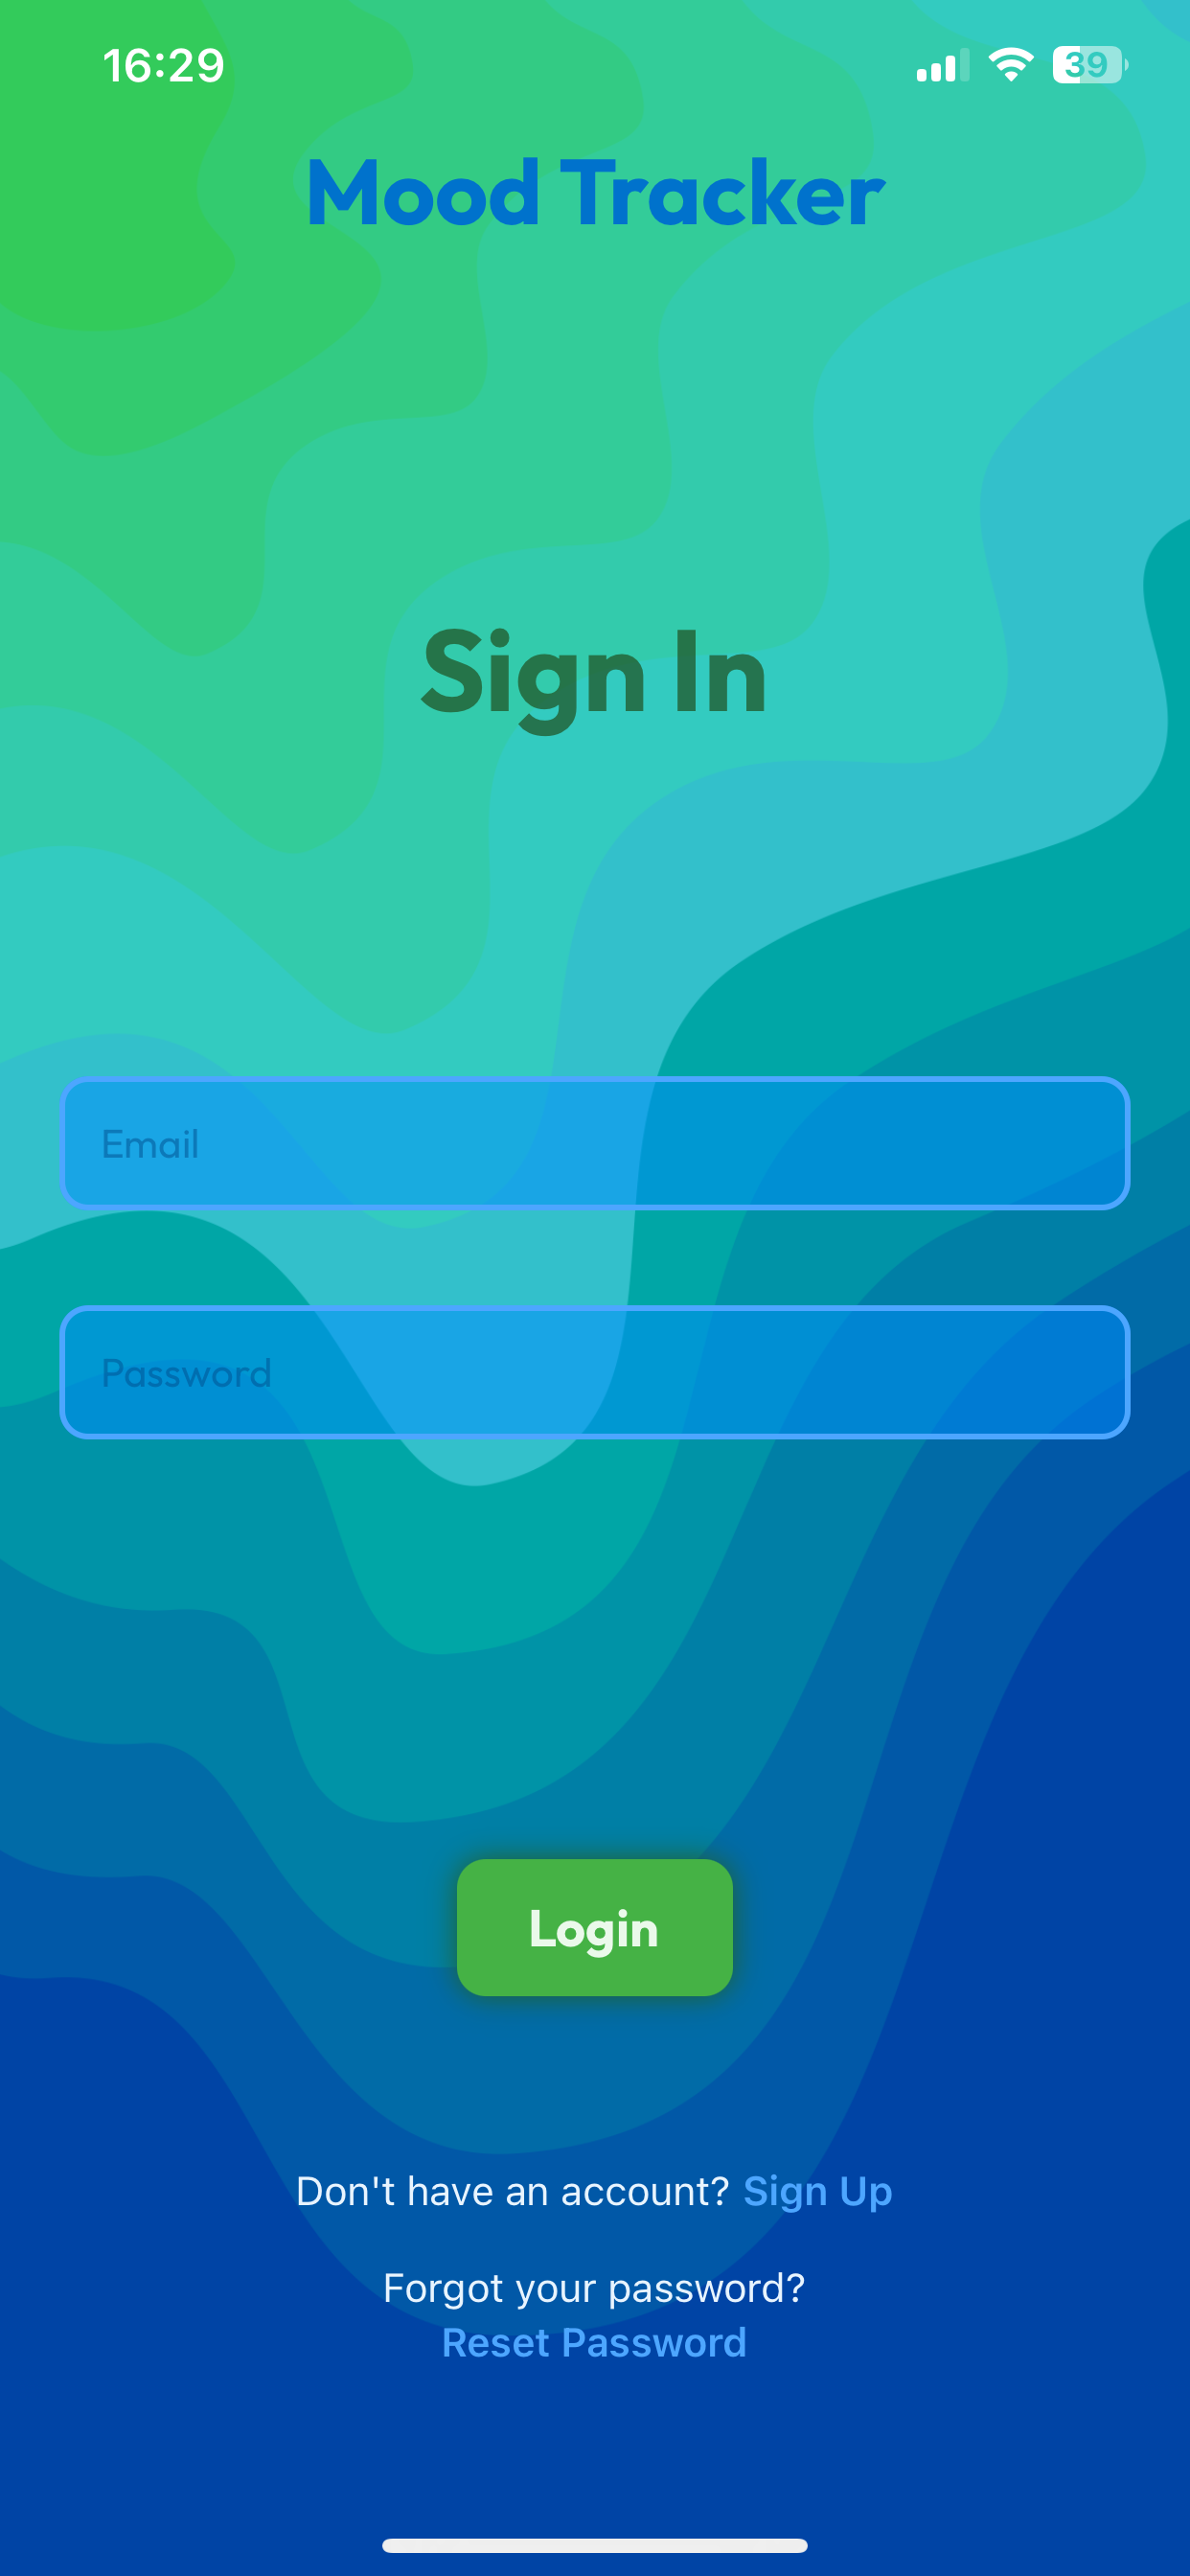
\includegraphics[scale=0.11]{figures/screenshots/Sign In-Up/1.PNG}\label{fig:sign-in-page}}
    \hspace{5mm}
    \subfloat[Sign Up]{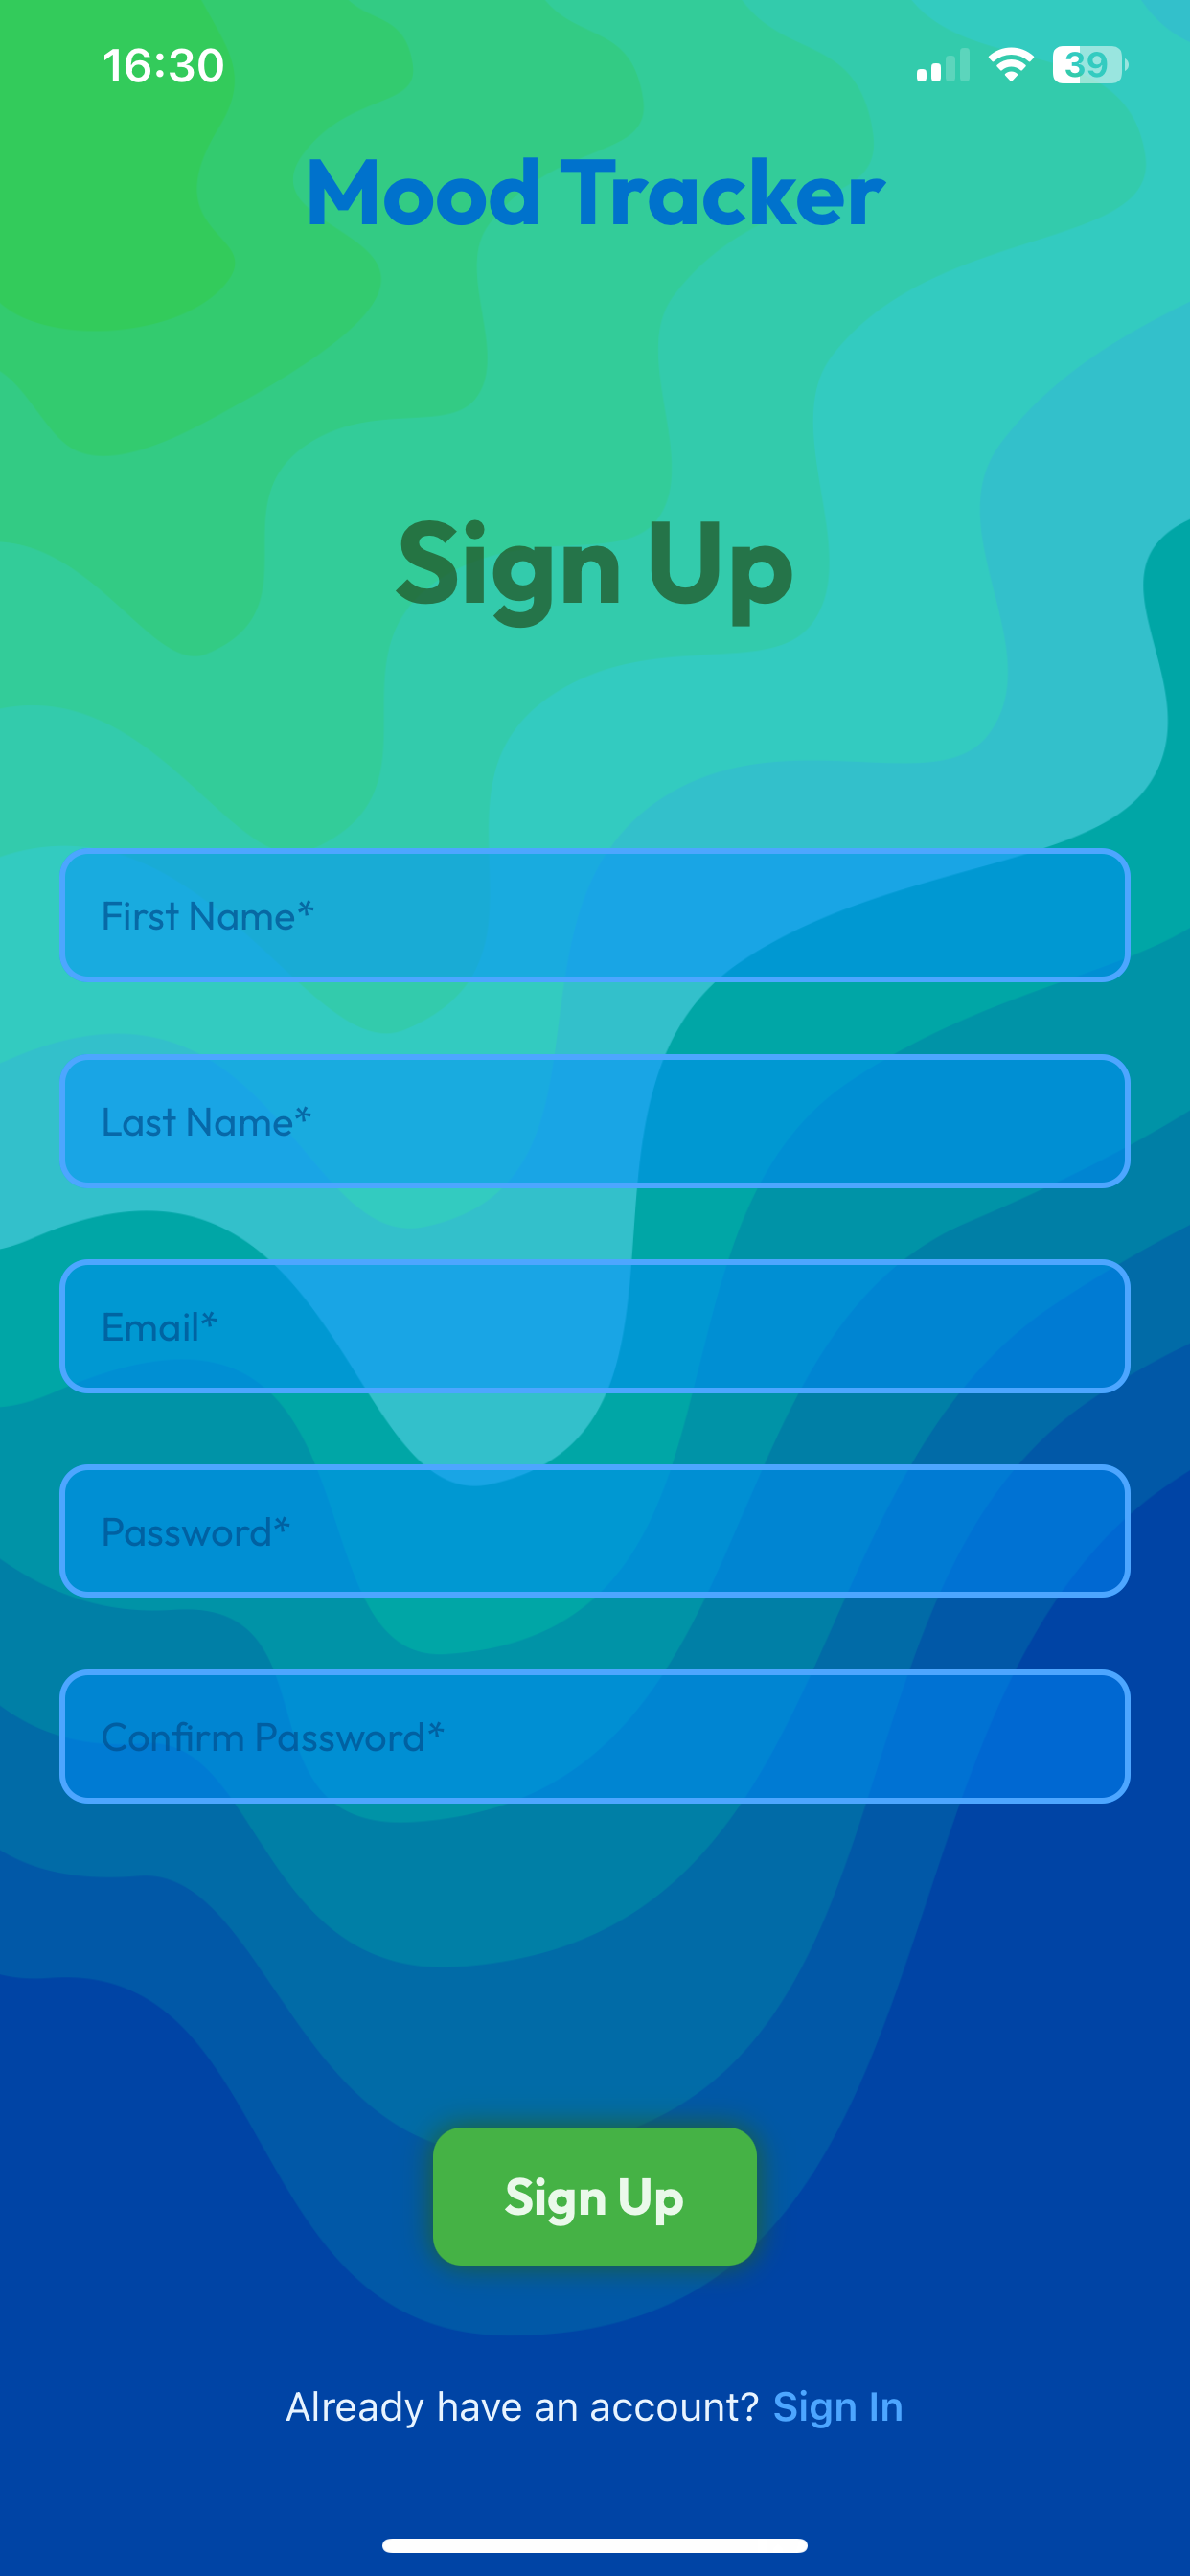
\includegraphics[scale=0.11]{figures/screenshots/Sign In-Up/2.PNG}\label{fig:sign-up-page}}
    \caption{Sign In/Up Screens}
\end{figure}
\FloatBarrier

\vspace{5mm}

\subsection{Password Reset}

\noindent \textbf{Step 1 [\ref{fig:password-reset-step-1}]} \\
The first step of the Password Reset process involves the user entering their email address to receive a password reset link. This screen includes a single input field labeled \textit{example@gmail.com}, where users are expected to type in the email address associated with their account. Below the input field, there is a blue button labeled ``Request Password Reset''. Users should click this button after entering their email address to initiate the password reset process.

\vspace{5mm}

\noindent \textbf{Step 2 [\ref{fig:password-reset-step-2}]} \\
After submitting the email address, user can see a success message confirming that a password reset email has been sent. The message is displayed in a pop-up dialog with the text ``Success! Password reset email sent successfully'' and an ``OK'' button. Clicking the ``OK'' button redirects the user back to the Sign In page, where they can proceed to log in after resetting their password.

\vspace{5mm}

\noindent \textbf{Step 3 [\ref{fig:password-reset-step-3}]} \\
The final step of the password reset process involves checking the user's email for the password reset link. The email contains a message with a link to reset the password, which usually includes the text ``Click the link below to reset your password:''. Users need to click on the provided link to complete the password reset procedure.\vspace{10mm} \\
Because of the limitations of the Expo environment, the deep linking doesn't work as expected, in order to be able to navigate to the ``Password Reset'' screen. But the implementation is correct and when the application is published properly (App Store or Google Play), the deeplinking is going to be modified and work accordingly.

\vspace{5mm}

\FloatBarrier
\begin{figure}[ht]
    \centering
    \subfloat[Step 1]{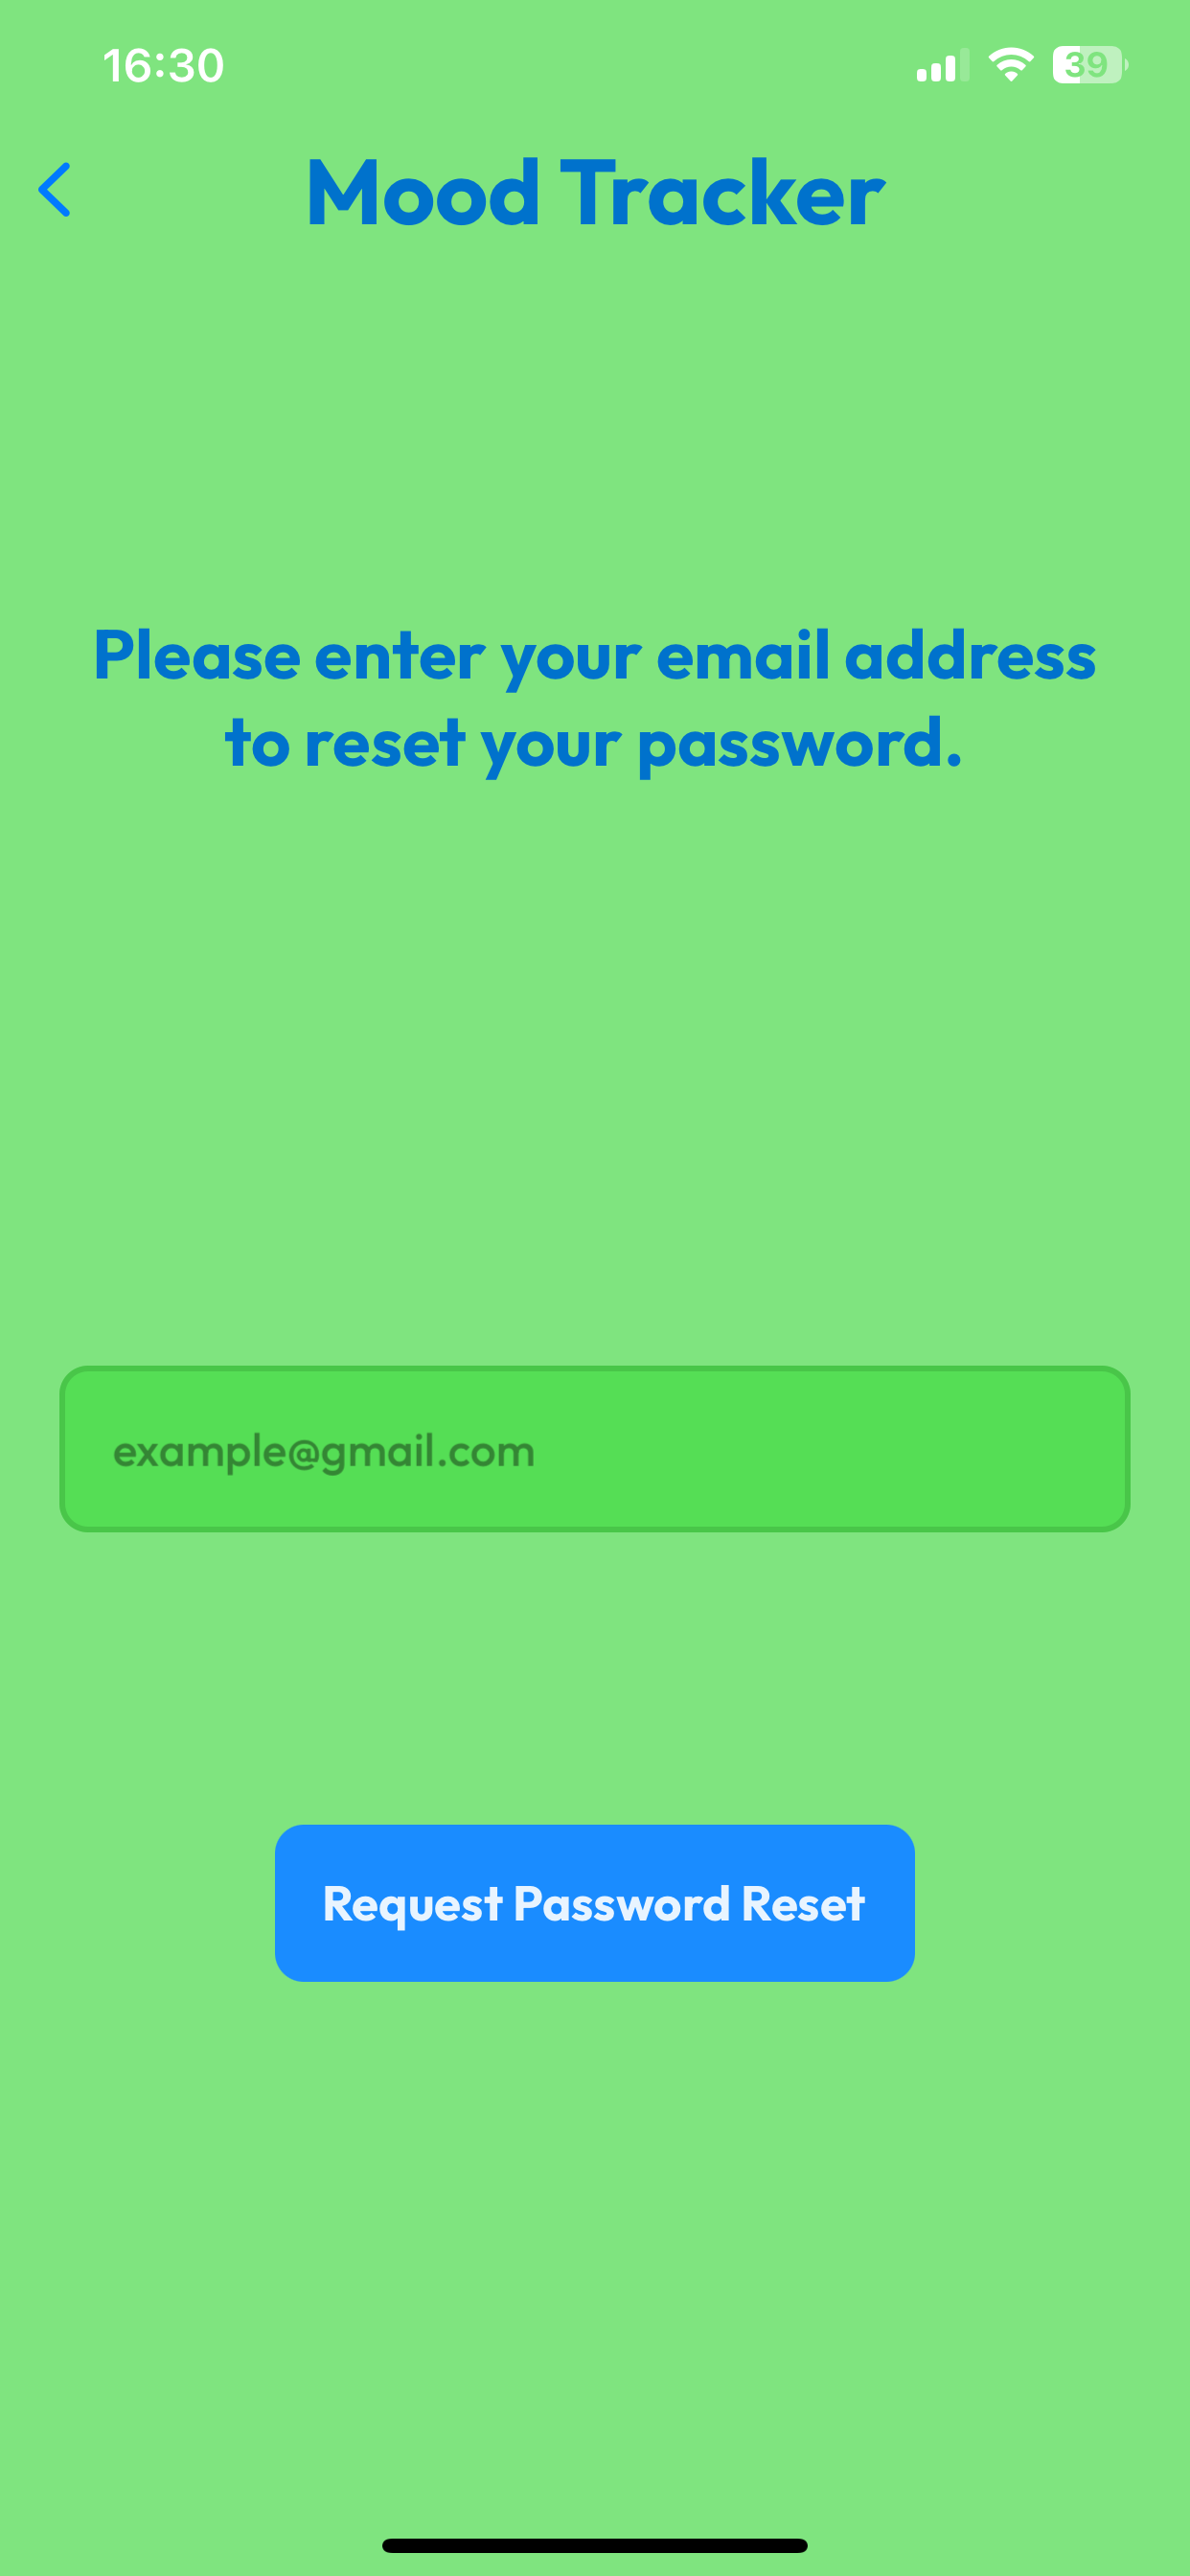
\includegraphics[scale=0.12]{figures/screenshots/Password Reset/1.PNG}\label{fig:password-reset-step-1}}
    \hspace{10mm}
    \subfloat[Step 2]{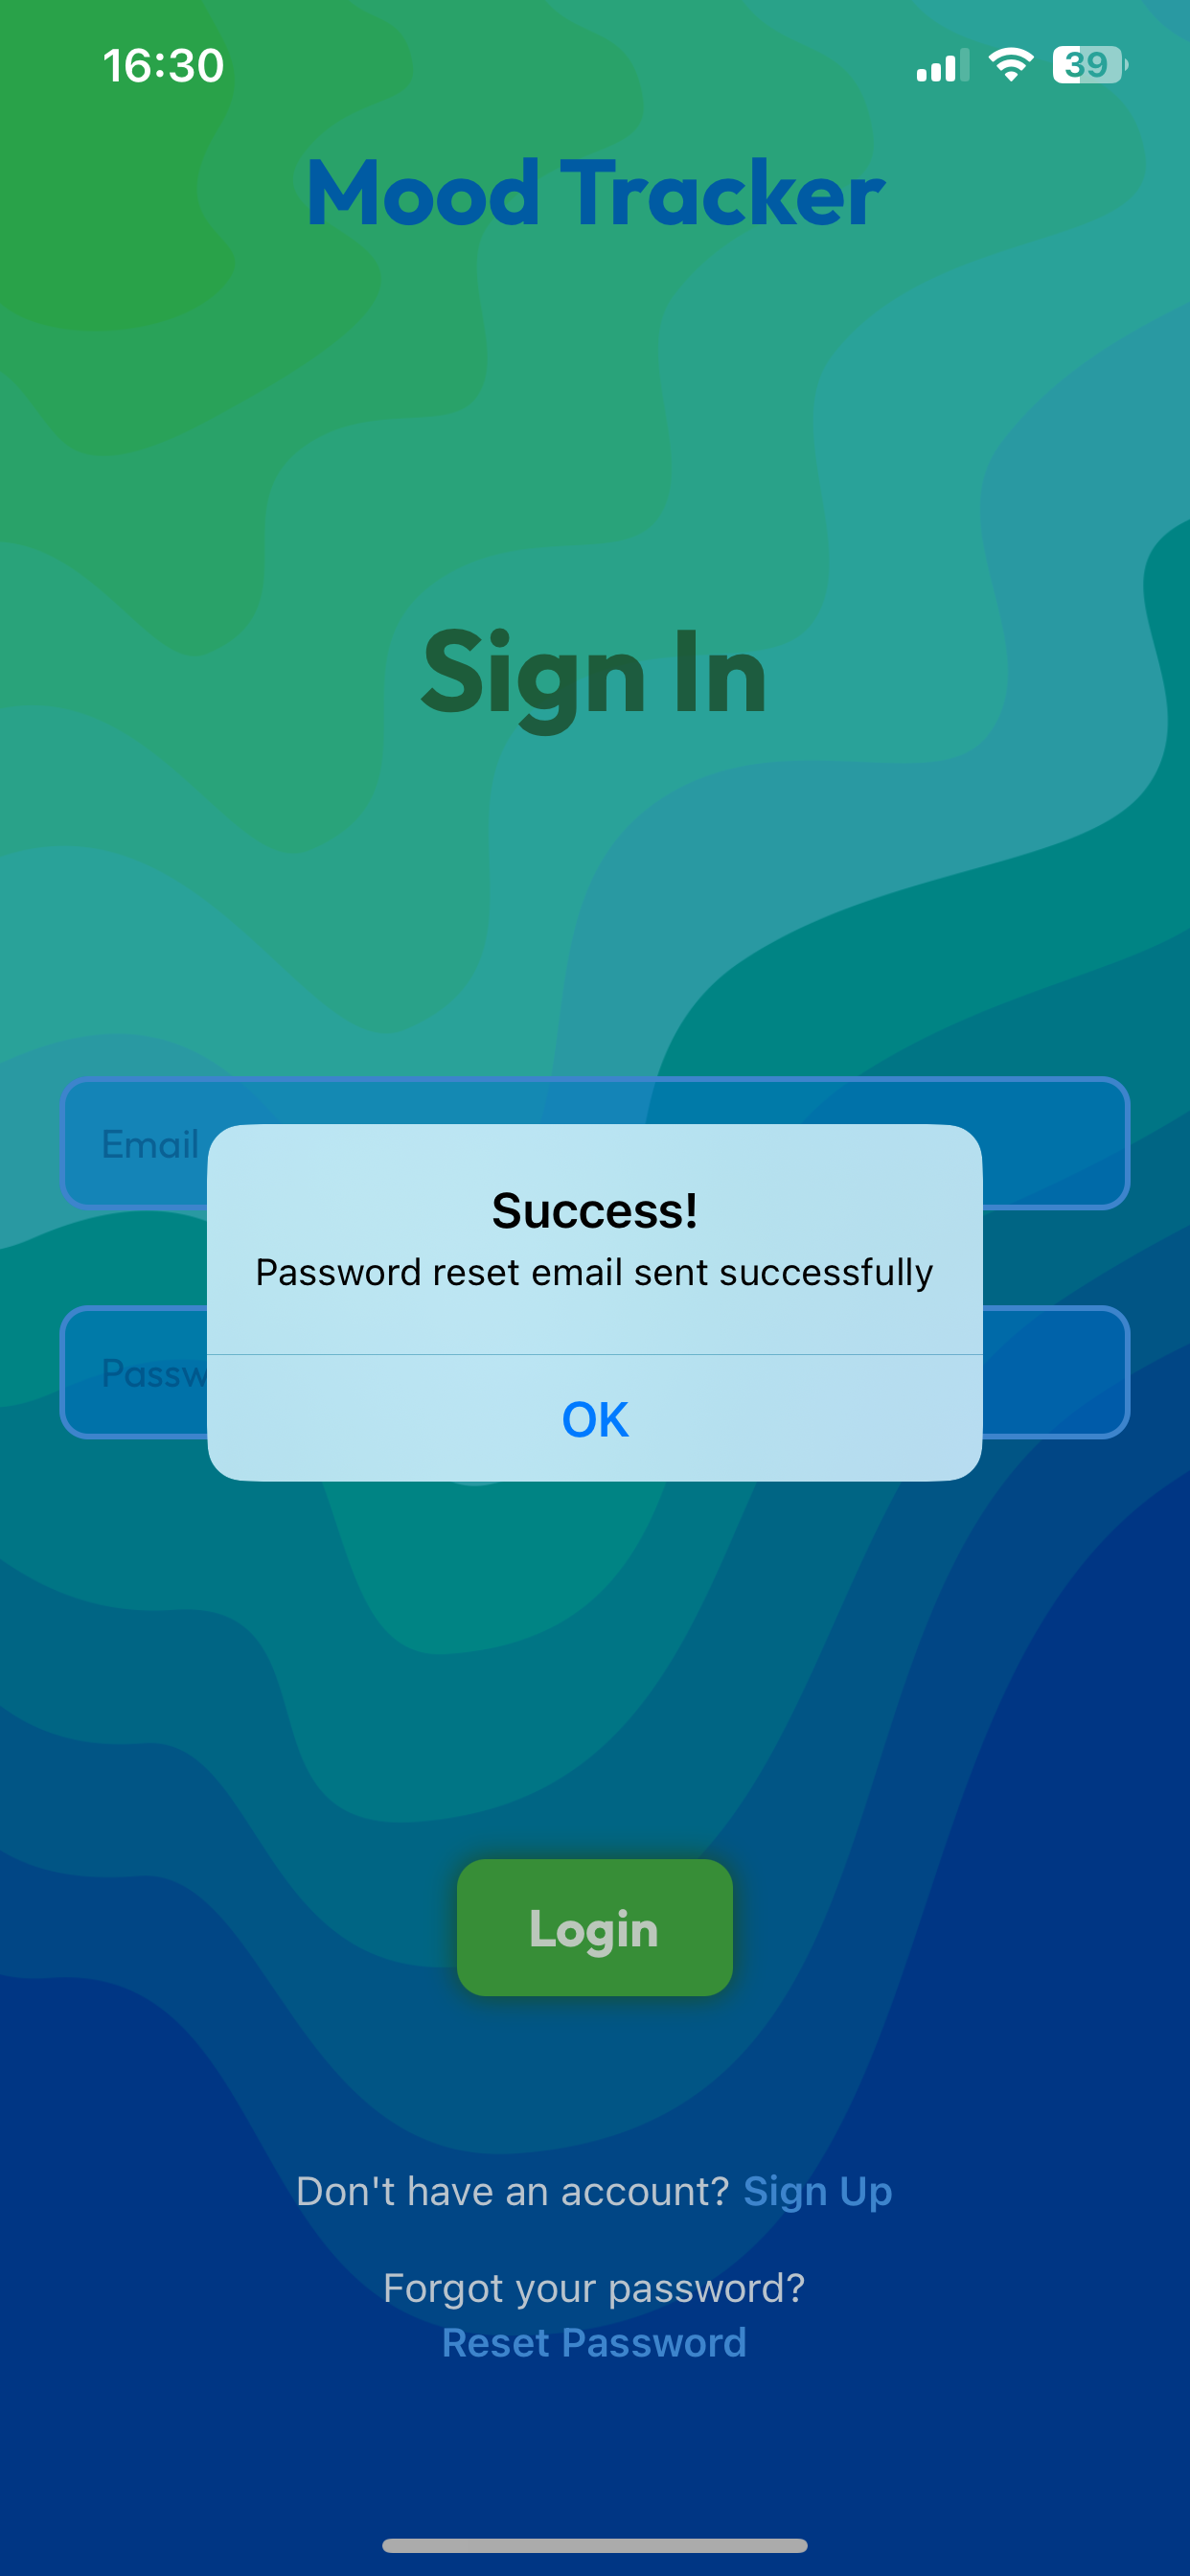
\includegraphics[scale=0.12]{figures/screenshots/Password Reset/2.PNG}\label{fig:password-reset-step-2}}
    \vspace{5mm}
\end{figure}
\FloatBarrier

\FloatBarrier
\begin{figure}[ht]\ContinuedFloat
    \centering
    \subfloat[Step 3]{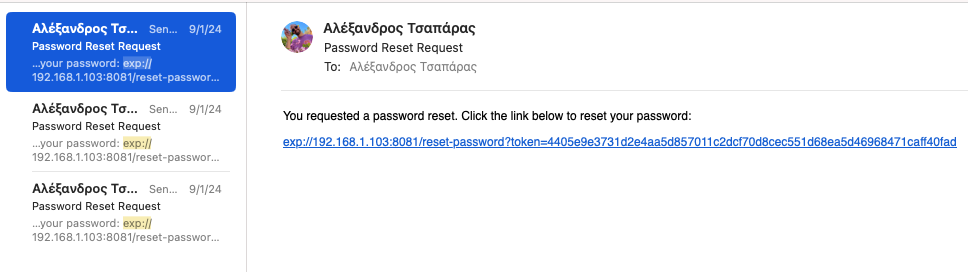
\includegraphics[scale=0.4]{figures/screenshots/Password Reset/Email Response.png}\label{fig:password-reset-step-3}}
    \caption{Procedure - Reset the password}
\end{figure}
\FloatBarrier

\vspace{5mm}

\subsection{Welcome Screen}

The Welcome Screen is displayed after the user has successfully signed in. This screen allows the user to input their current mood by selecting one of the available mood options. The screen also features a personalized greeting message like ``Hello, Alexandros'' (or the user's name respectively), followed by a prompt asking, ``How are you feeling today?''. Below the prompt, there are five mood options represented by different emoticons, ranging from `awful' to `happy'.\vspace{5mm} \\
After choosing a mood, the user can either press the ``Continue'' button to proceed with the selected mood or press the ``Skip'' button to bypass this step. If the ``Skip'' button is pressed, a confirmation dialog appears, asking if the user is sure they want to skip recording their welcome mood. This action puts the mood `nothing' to the users welcome mood.\vspace{5mm} \\
Different variations of the Welcome Screen exist, which include diverse backgrounds and themes depending every time the user logs in the application. The following images showcase these variations, as well as the functionalities available on this screen.

\vspace{5mm}

\FloatBarrier
\begin{figure}[ht]
    \centering
    \subfloat[Variation 1]{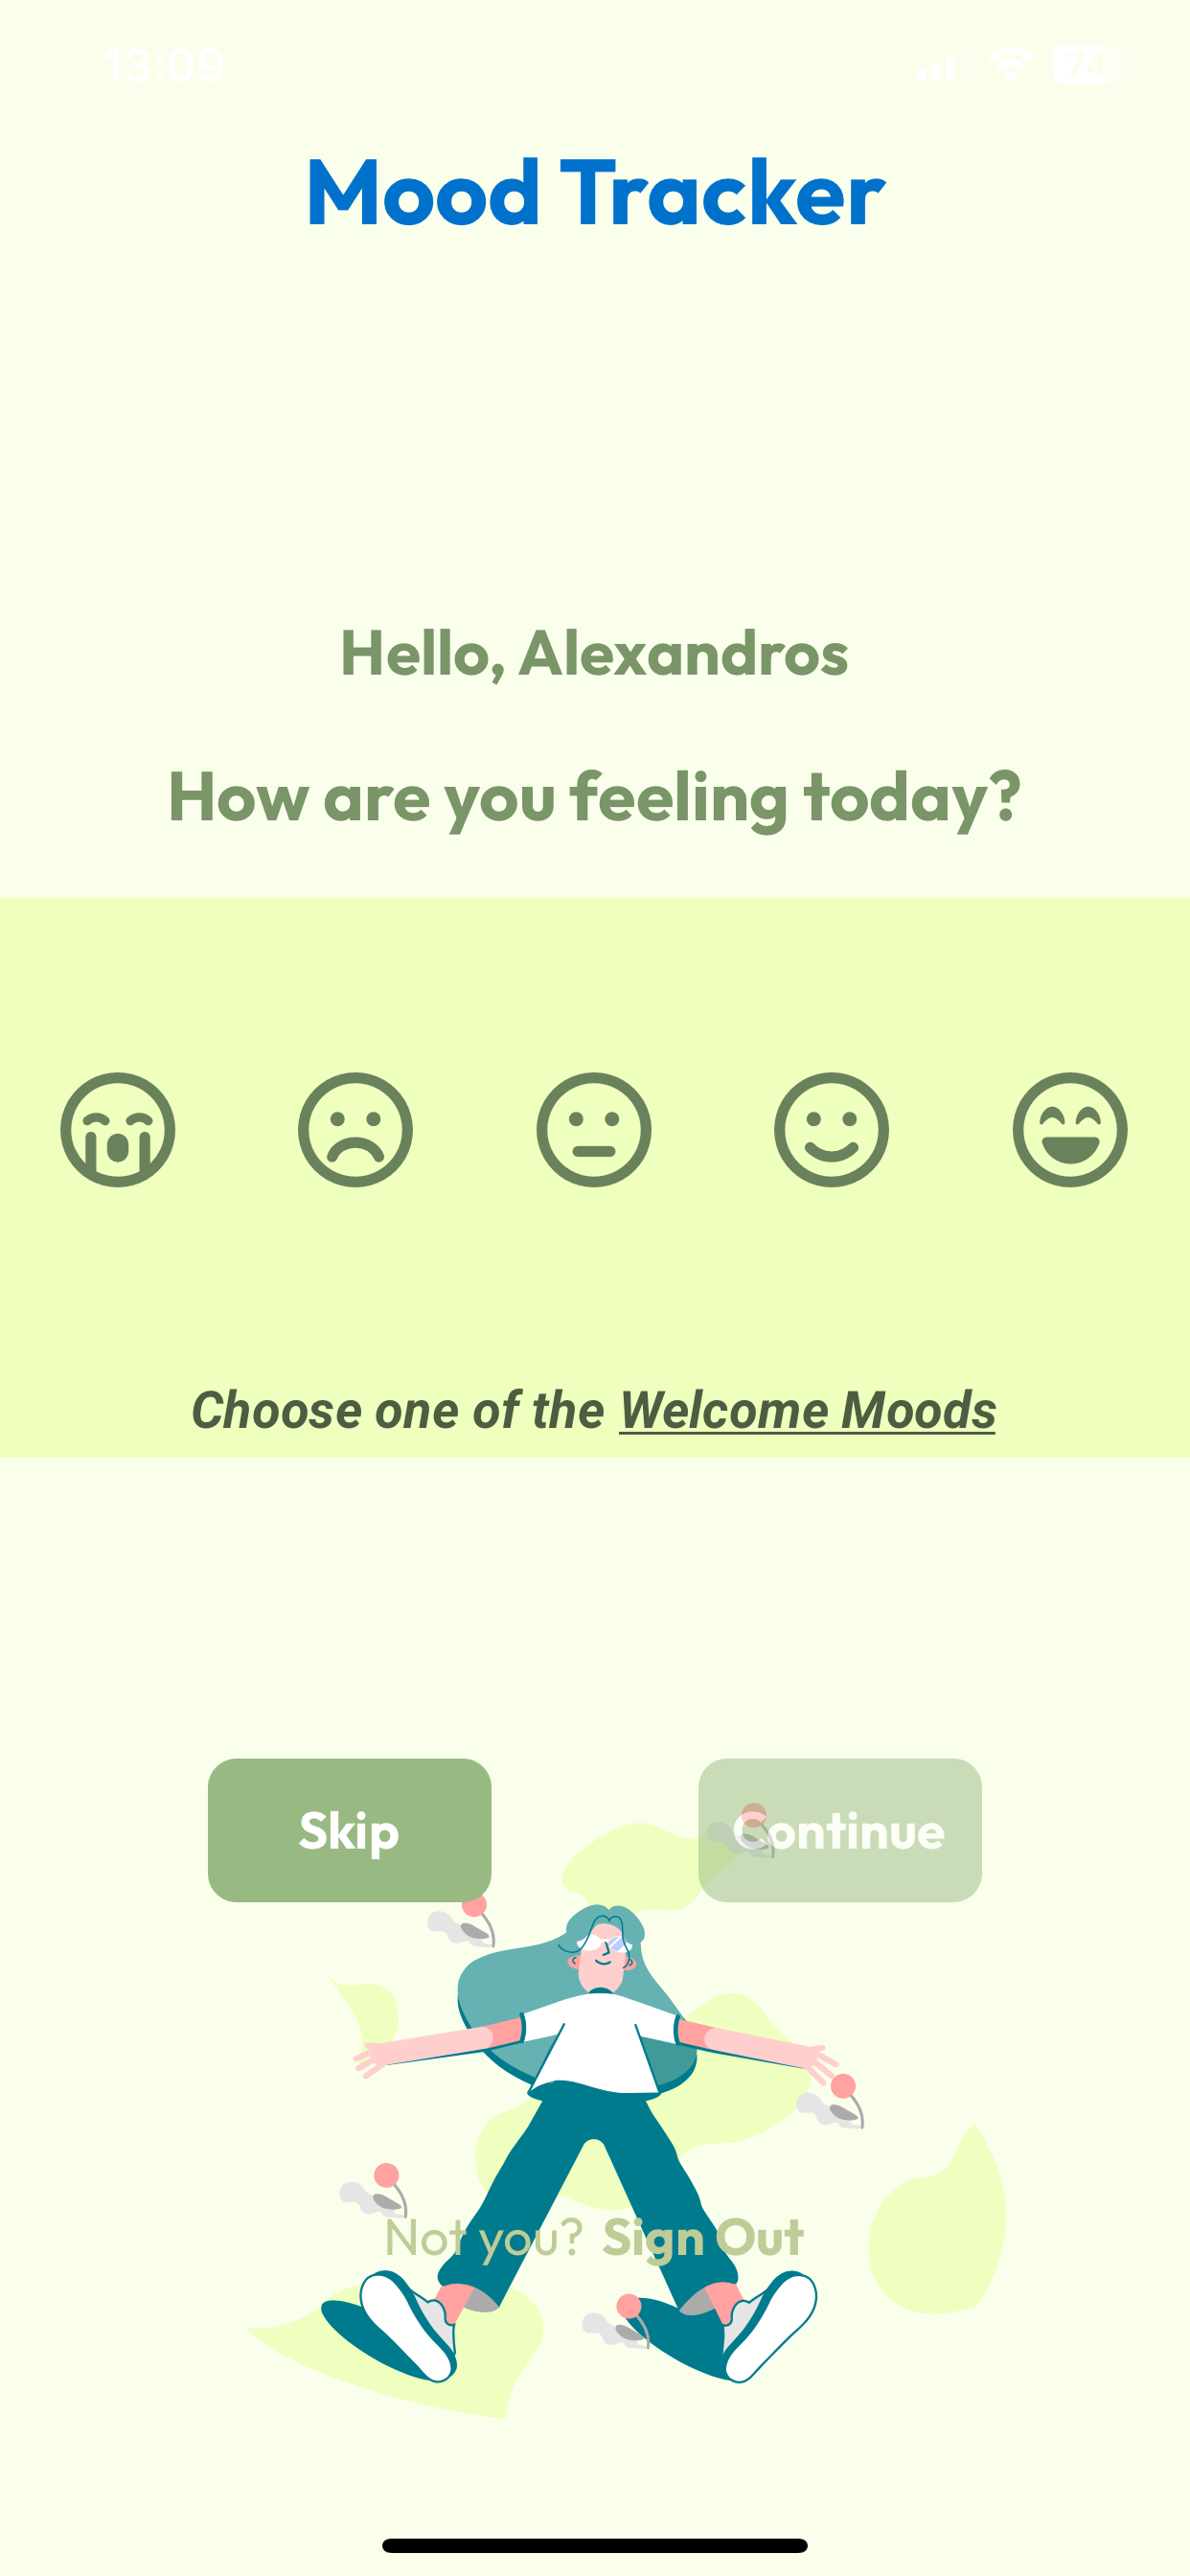
\includegraphics[scale=0.11]{figures/screenshots/Welcome Screen/1.PNG}\label{fig:welcome-variation-1}}
    \hfill
    \subfloat[Variation 2]{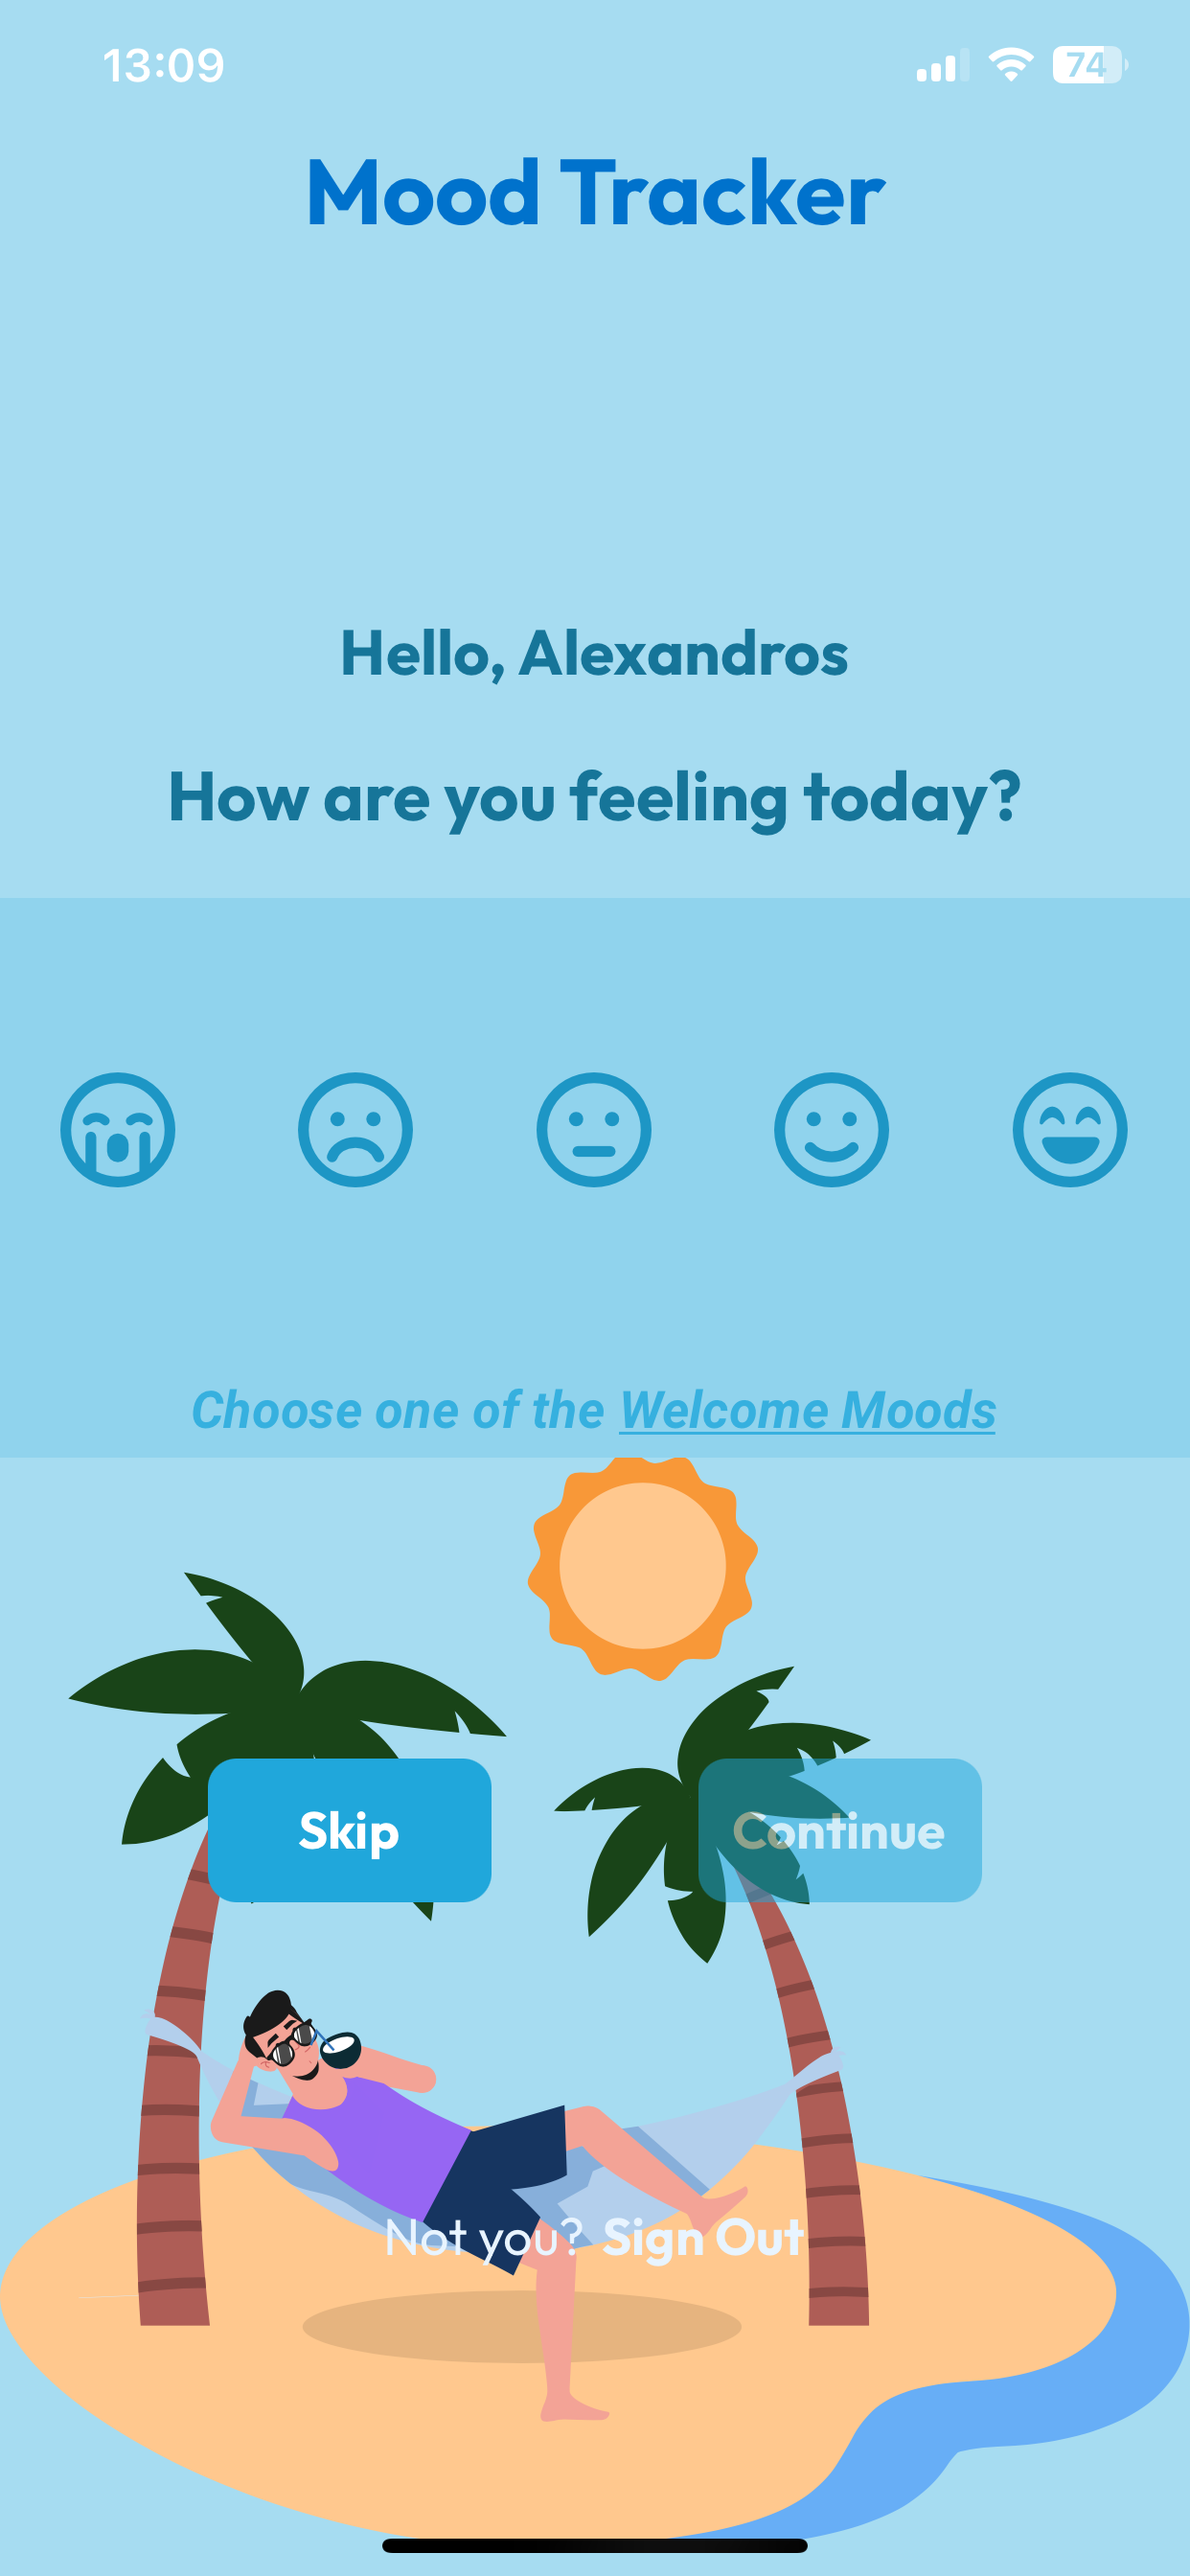
\includegraphics[scale=0.11]{figures/screenshots/Welcome Screen/2.PNG}\label{fig:welcome-variation-2}}
    \hfill
    \subfloat[Variation 3]{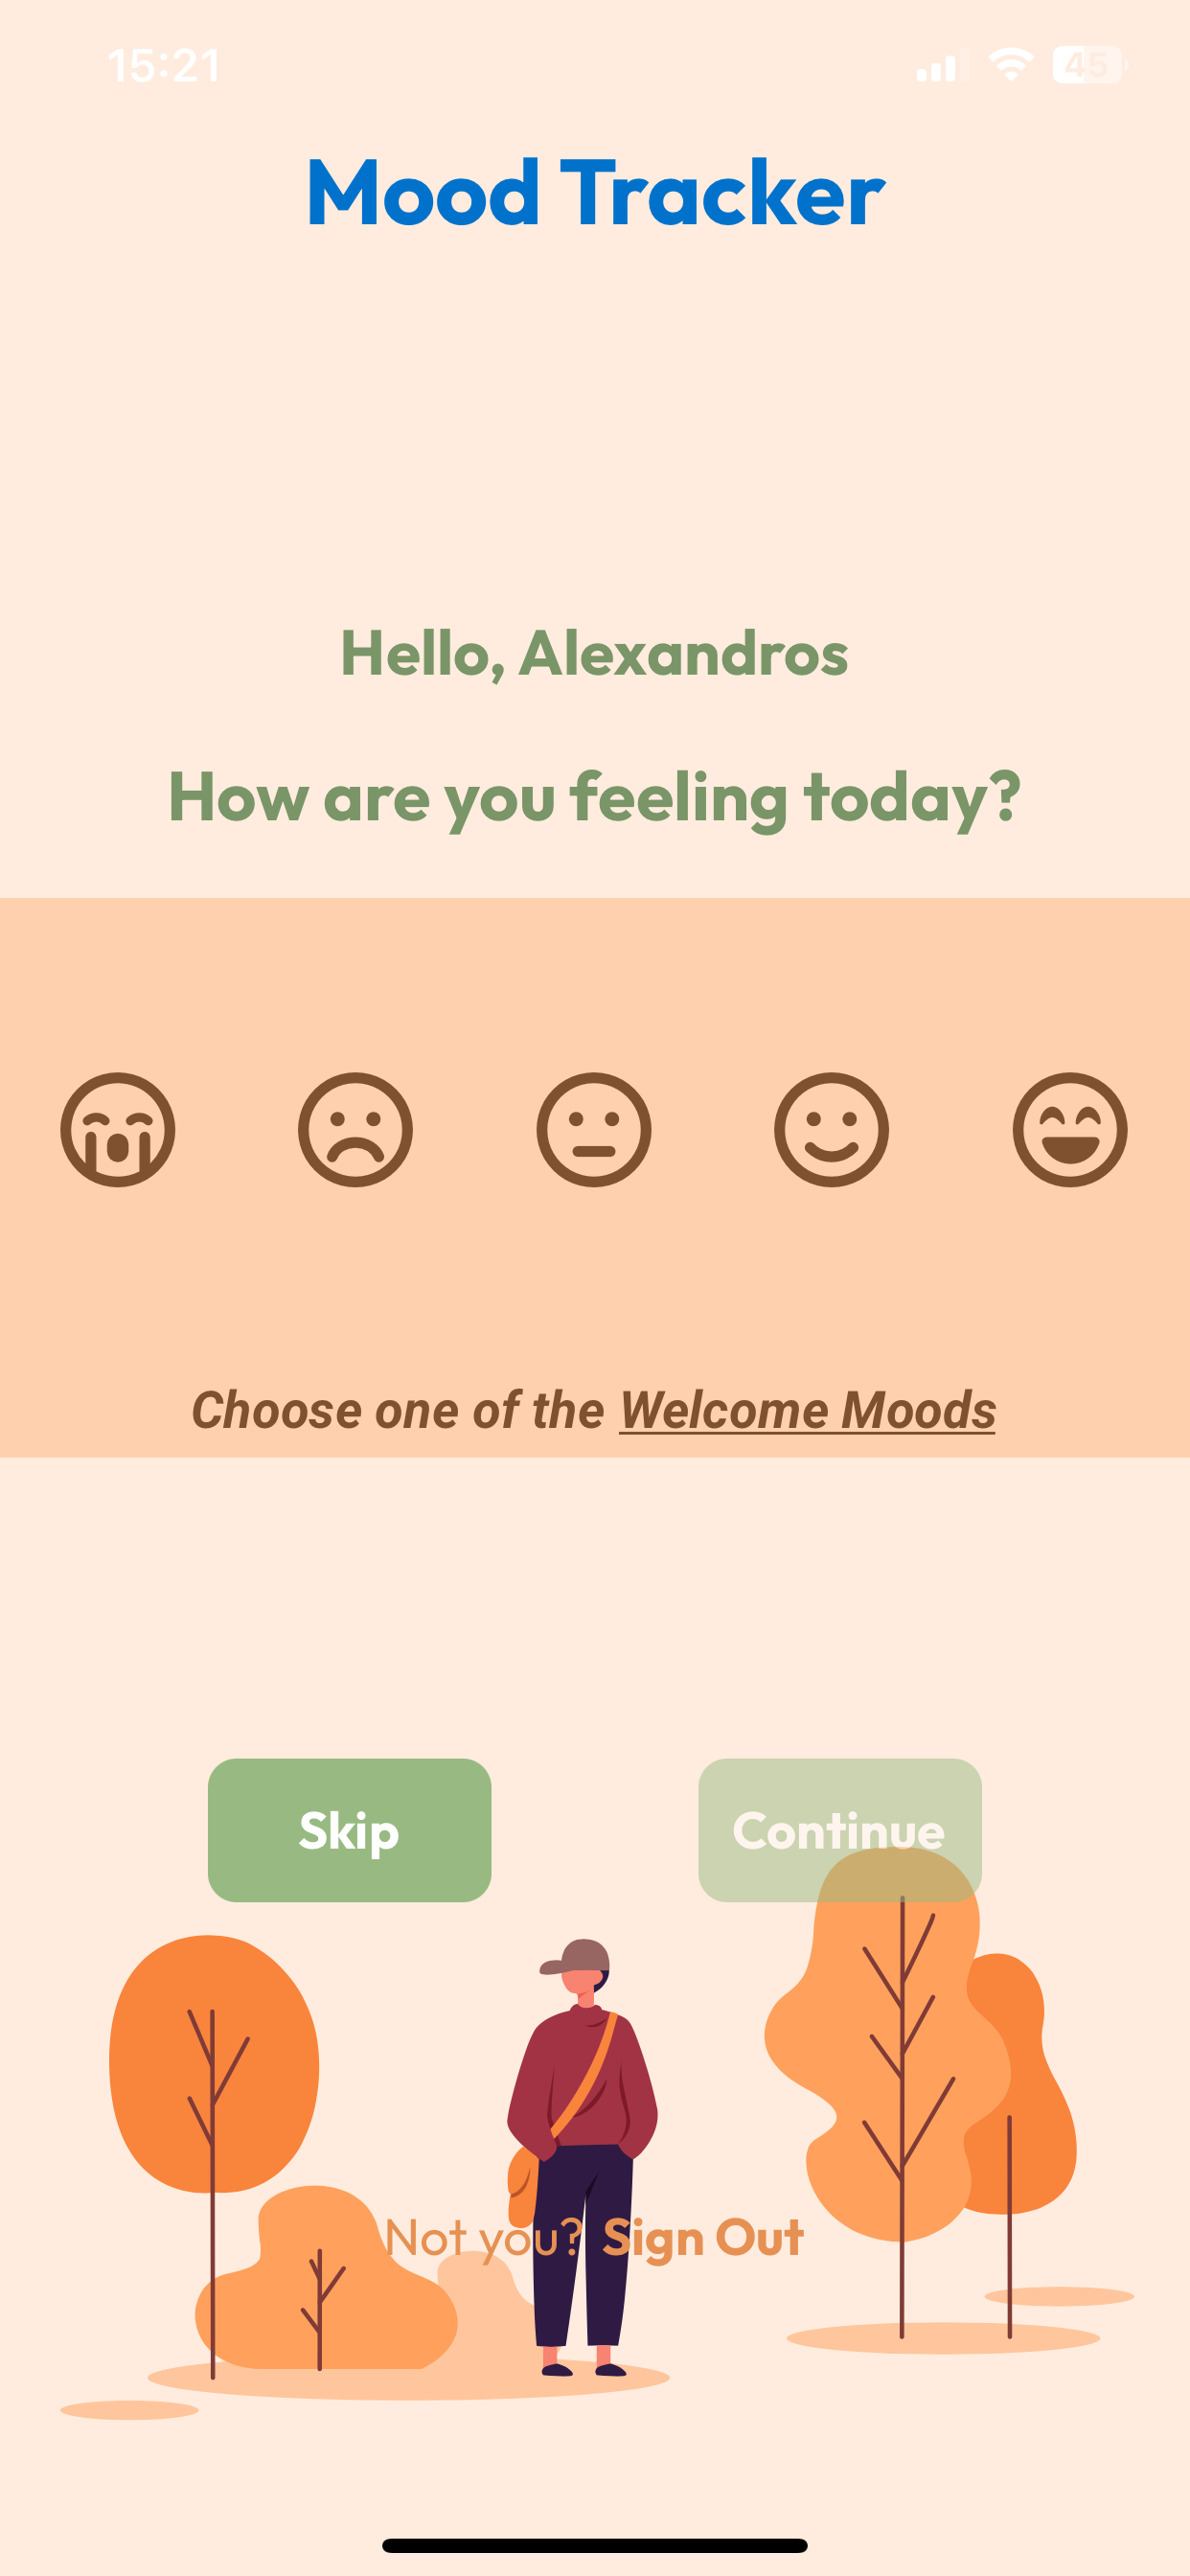
\includegraphics[scale=0.11]{figures/screenshots/Welcome Screen/3.PNG}\label{fig:welcome-variation-3}}
\end{figure}
\FloatBarrier

\FloatBarrier
\begin{figure}[ht]\ContinuedFloat
    \centering
    \subfloat[Variation 4]{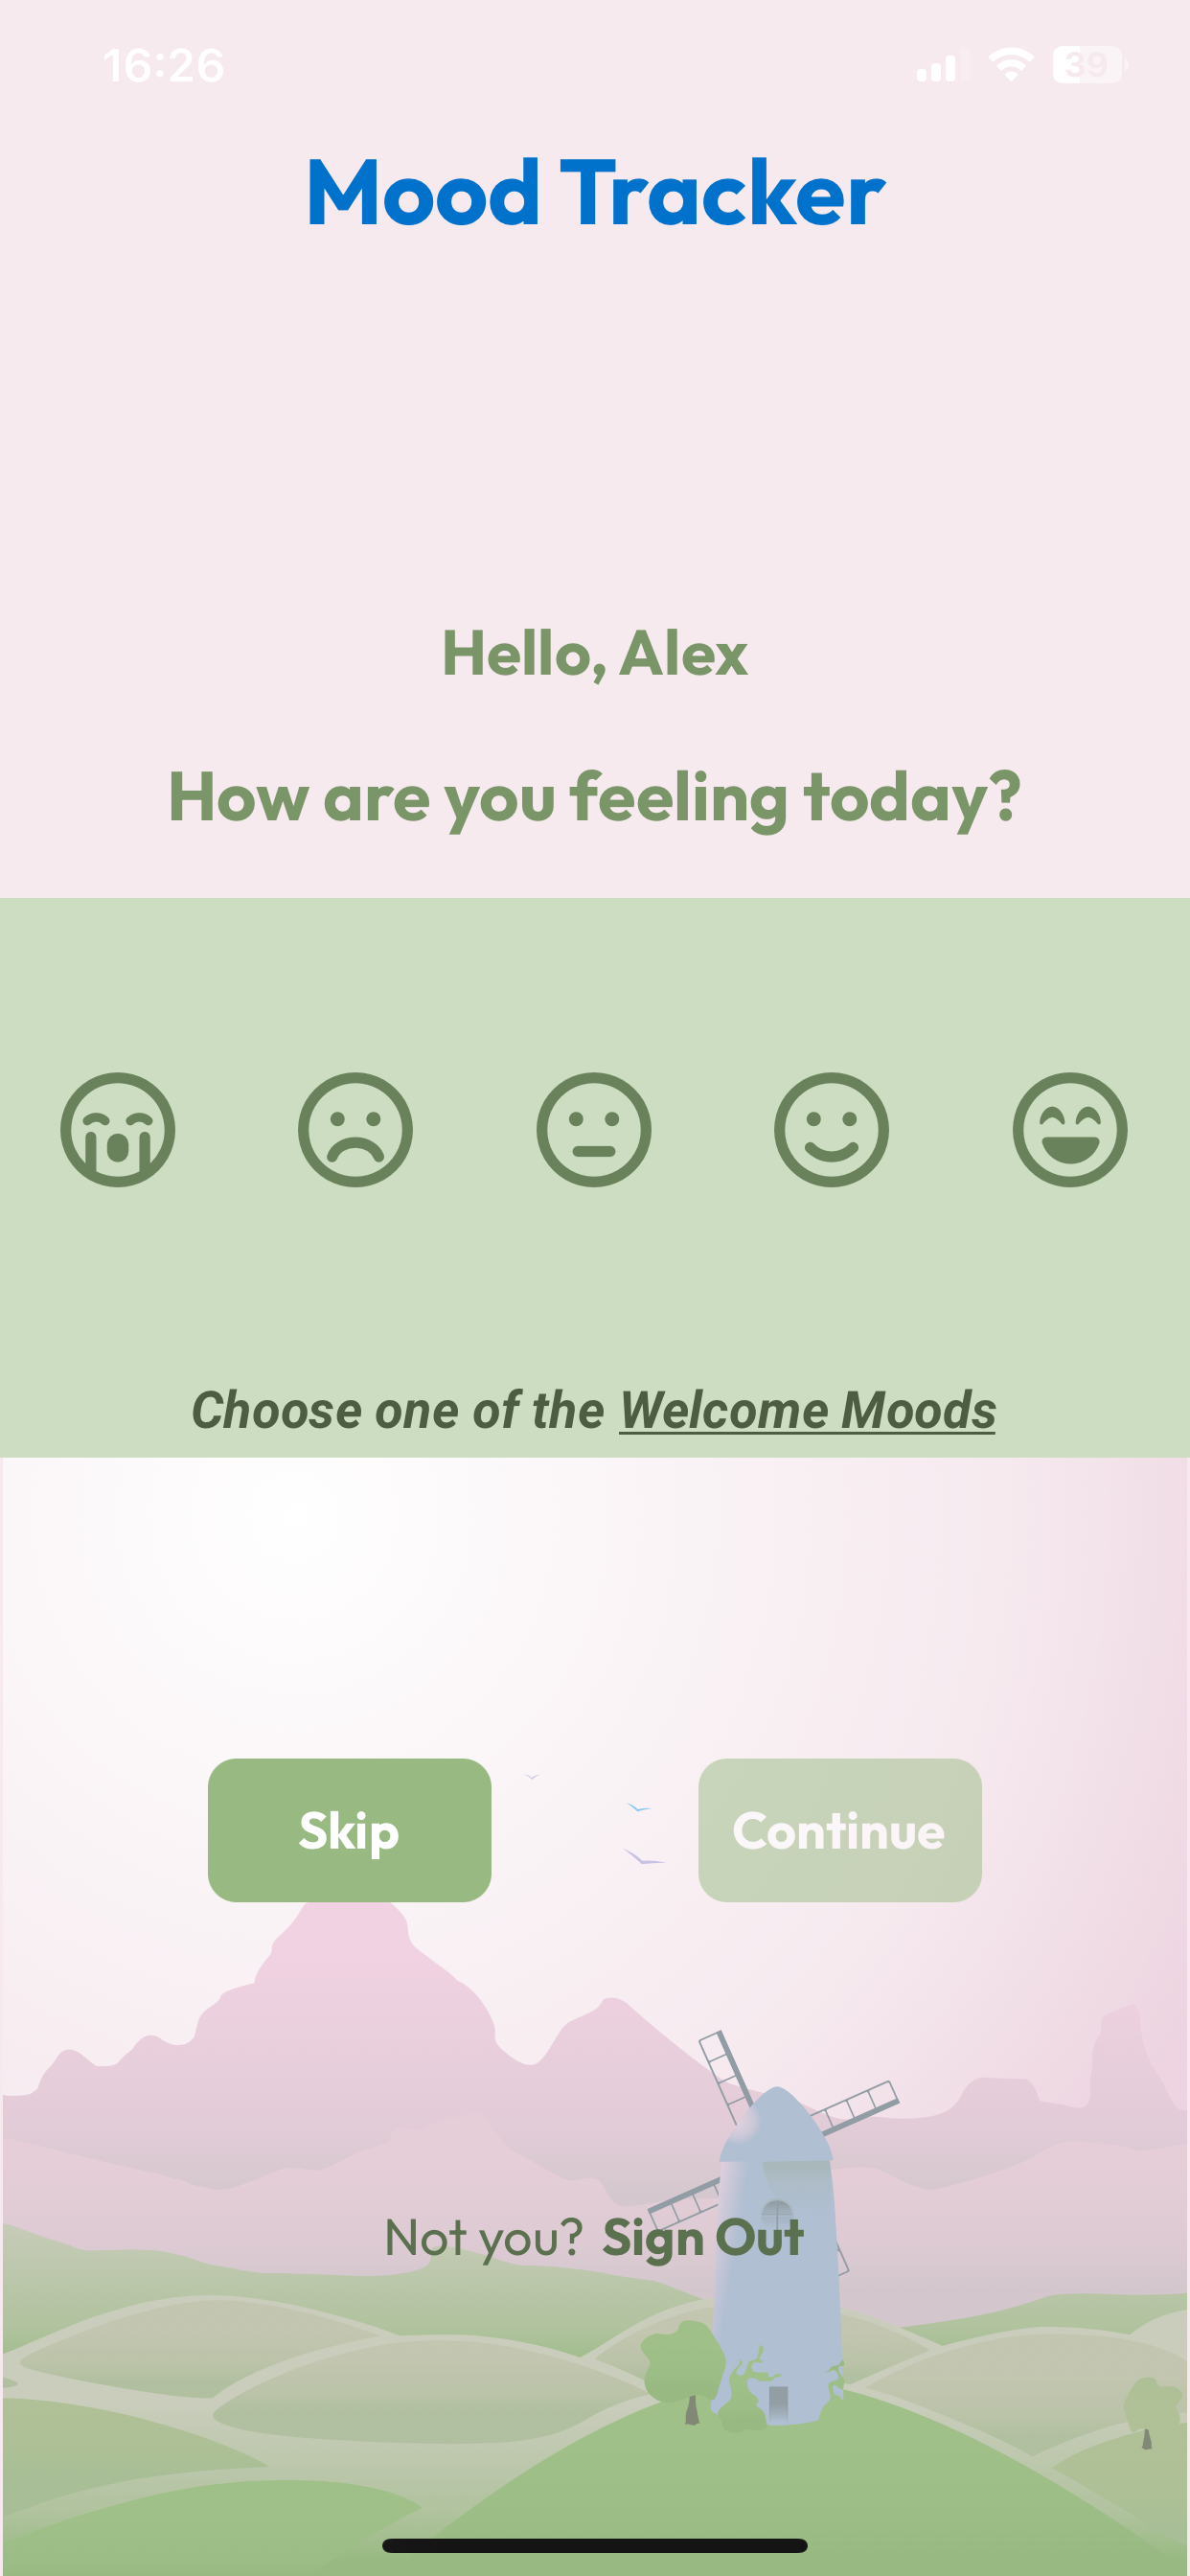
\includegraphics[scale=0.11]{figures/screenshots/Welcome Screen/4.PNG}\label{fig:welcome-variation-4}}
    \hspace{10mm}
    \subfloat[Variation 5]{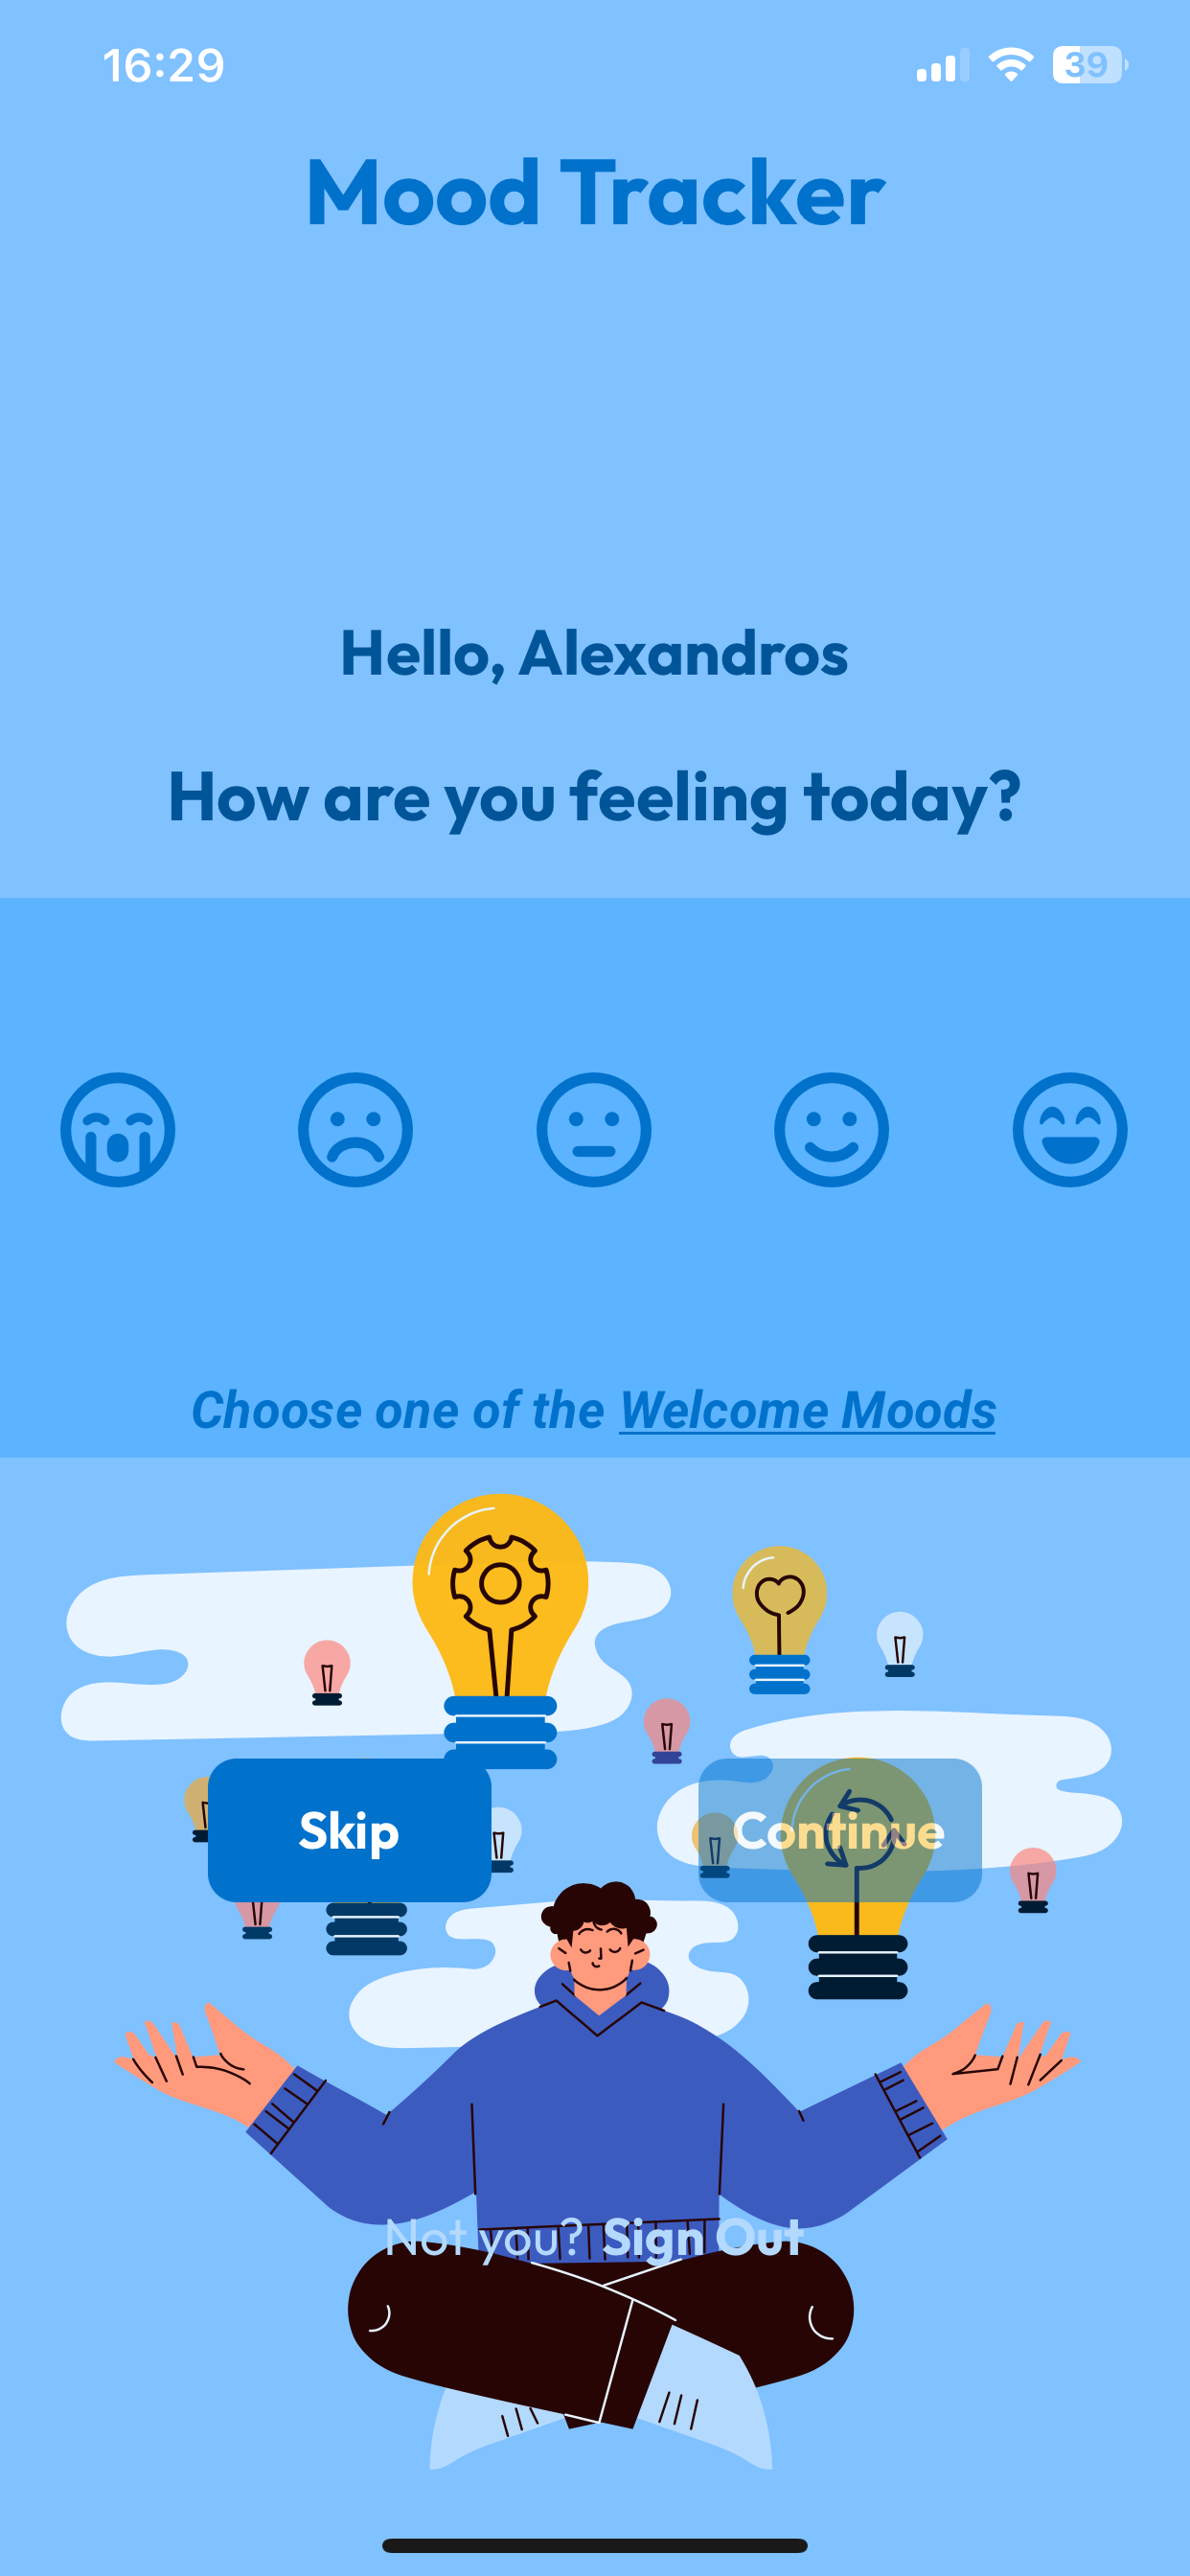
\includegraphics[scale=0.11]{figures/screenshots/Welcome Screen/8.PNG}\label{fig:welcome-variation-5}}
    \caption{Welcome Screen Variations}
\end{figure}
\FloatBarrier

\vspace{5mm}

\FloatBarrier
\begin{figure}[ht]
    \centering
    \subfloat[``Neutral'' emotion selected]{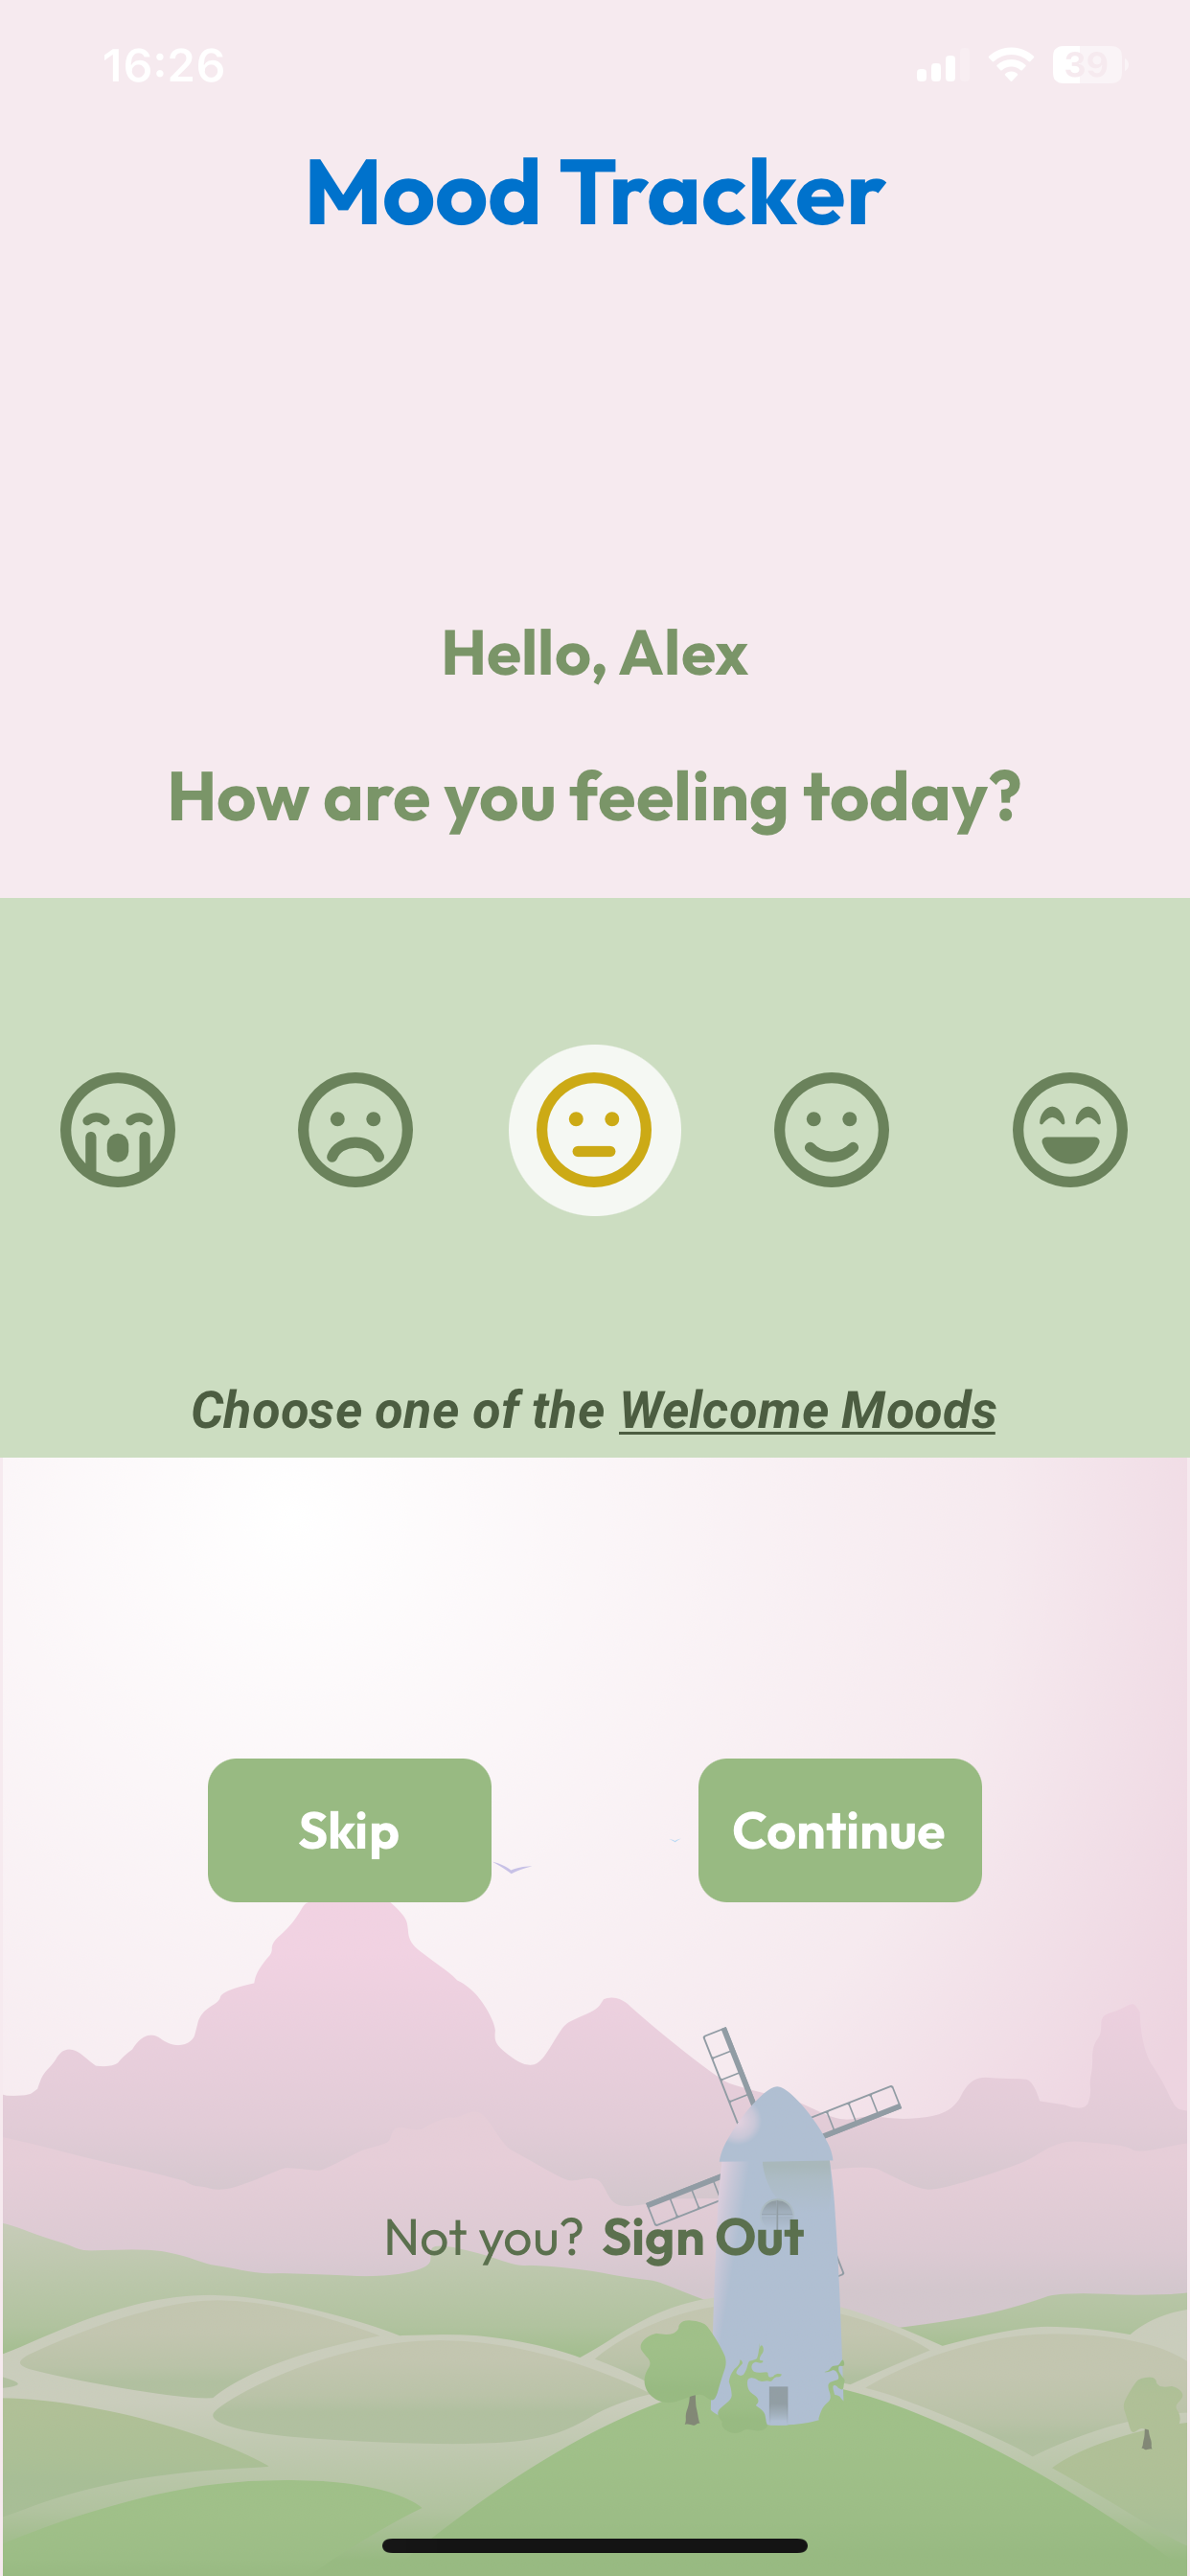
\includegraphics[scale=0.11]{figures/screenshots/Welcome Screen/5.PNG}\label{fig:neutral-selected}}
    \hfill
    \subfloat[``Happy'' emotion selected]{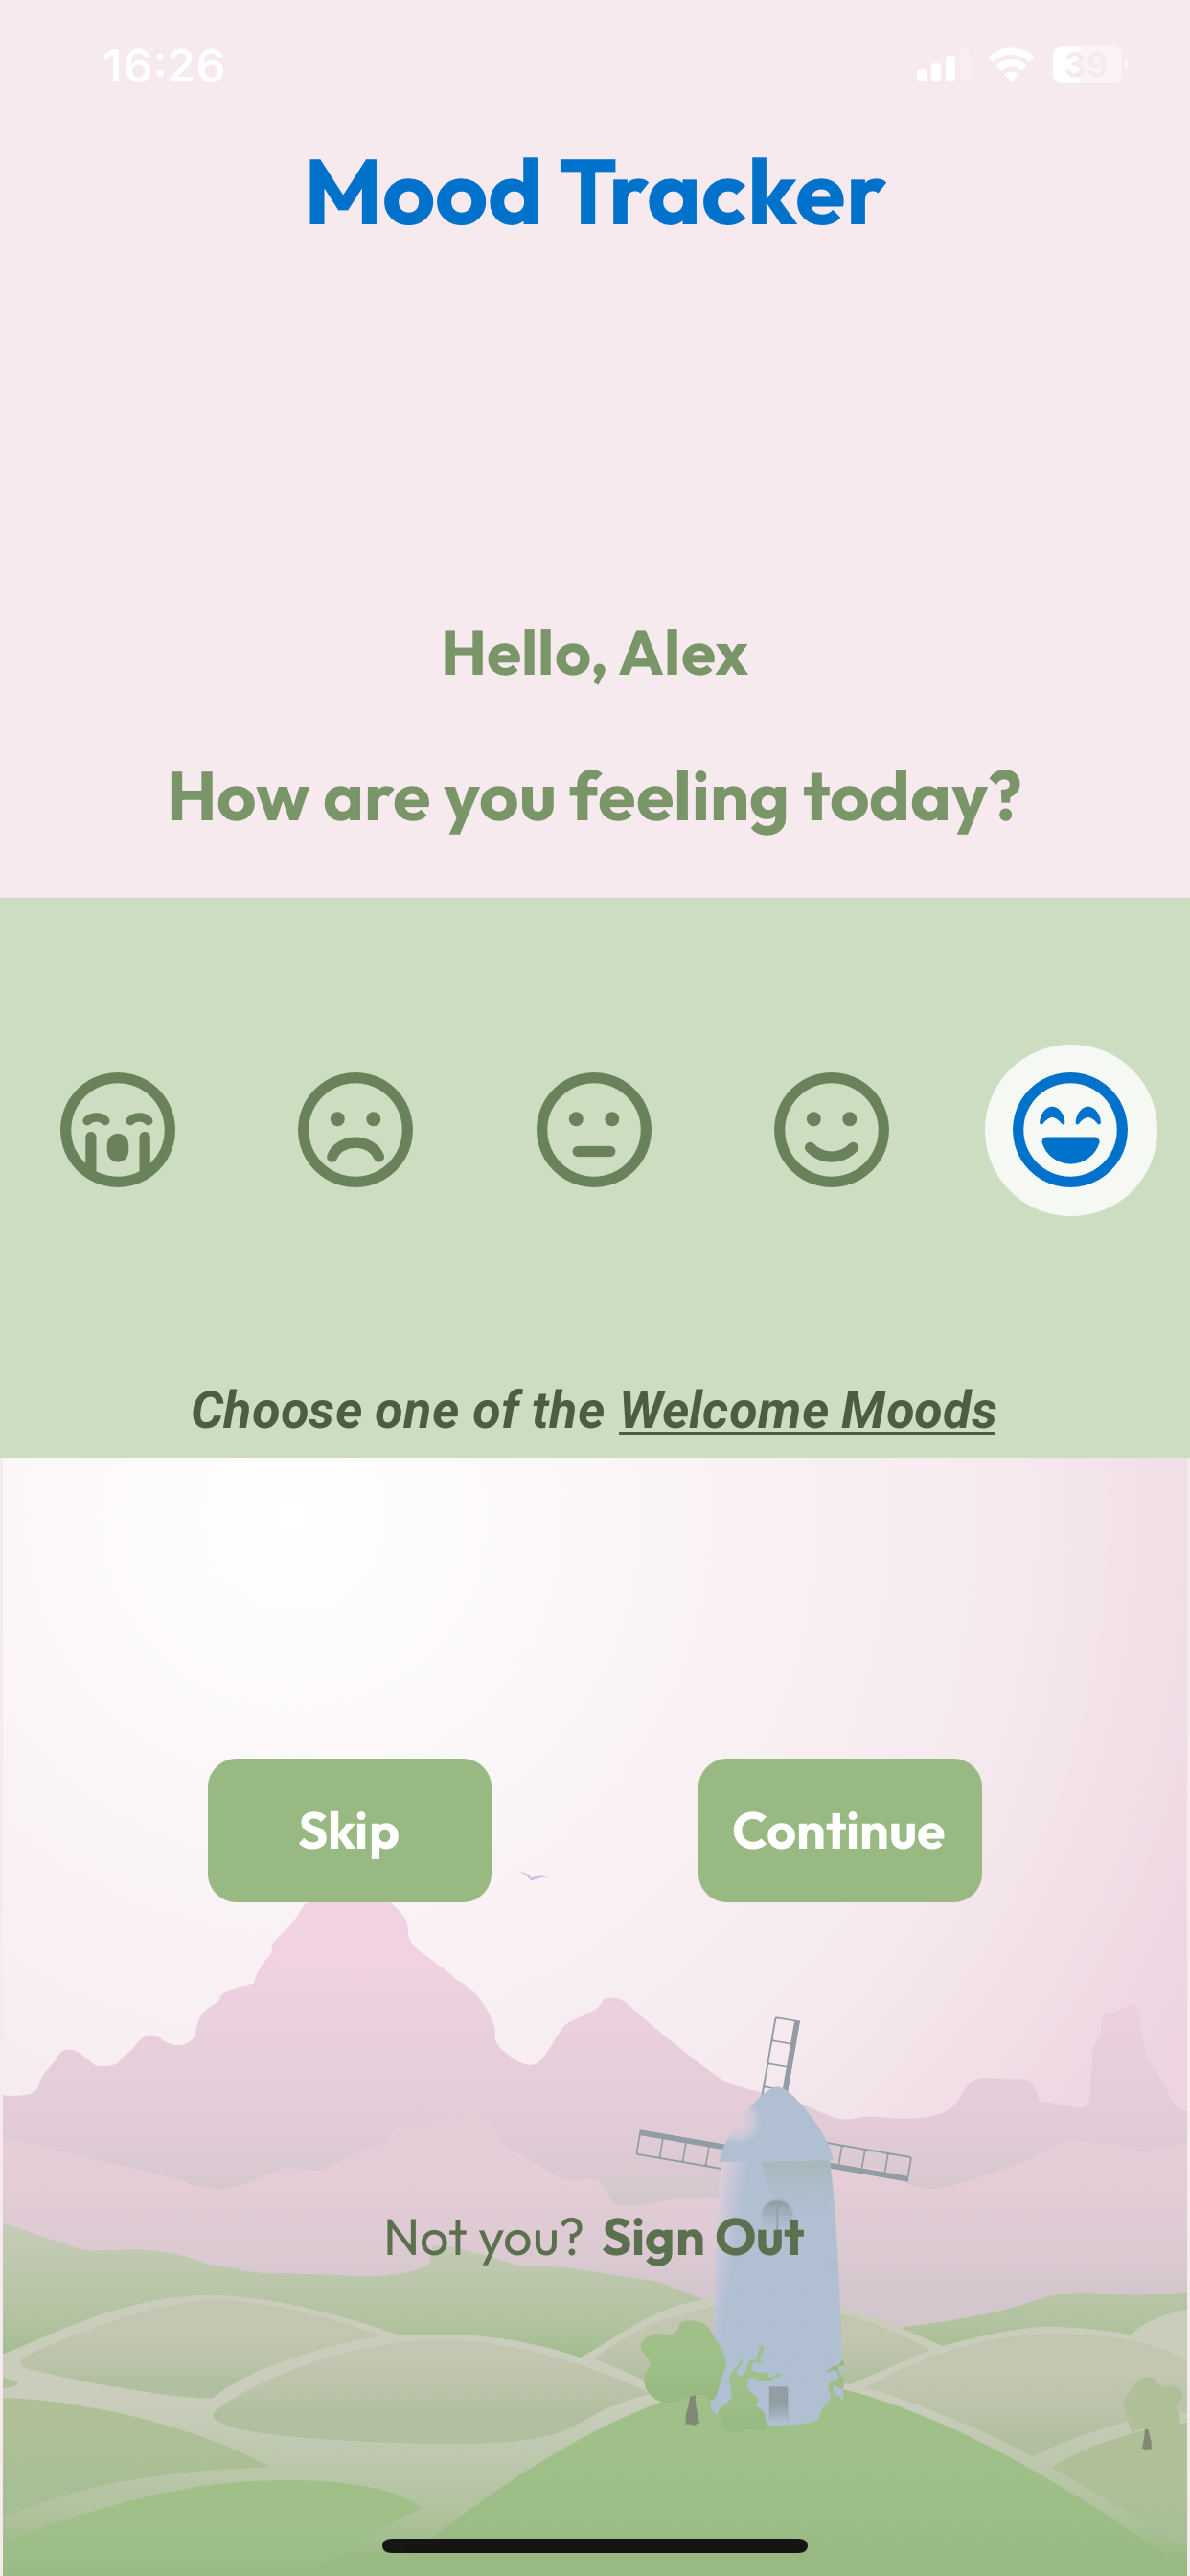
\includegraphics[scale=0.11]{figures/screenshots/Welcome Screen/6.PNG}\label{fig:happy-selected}}
    \hfill
    \subfloat[Skip procedure]{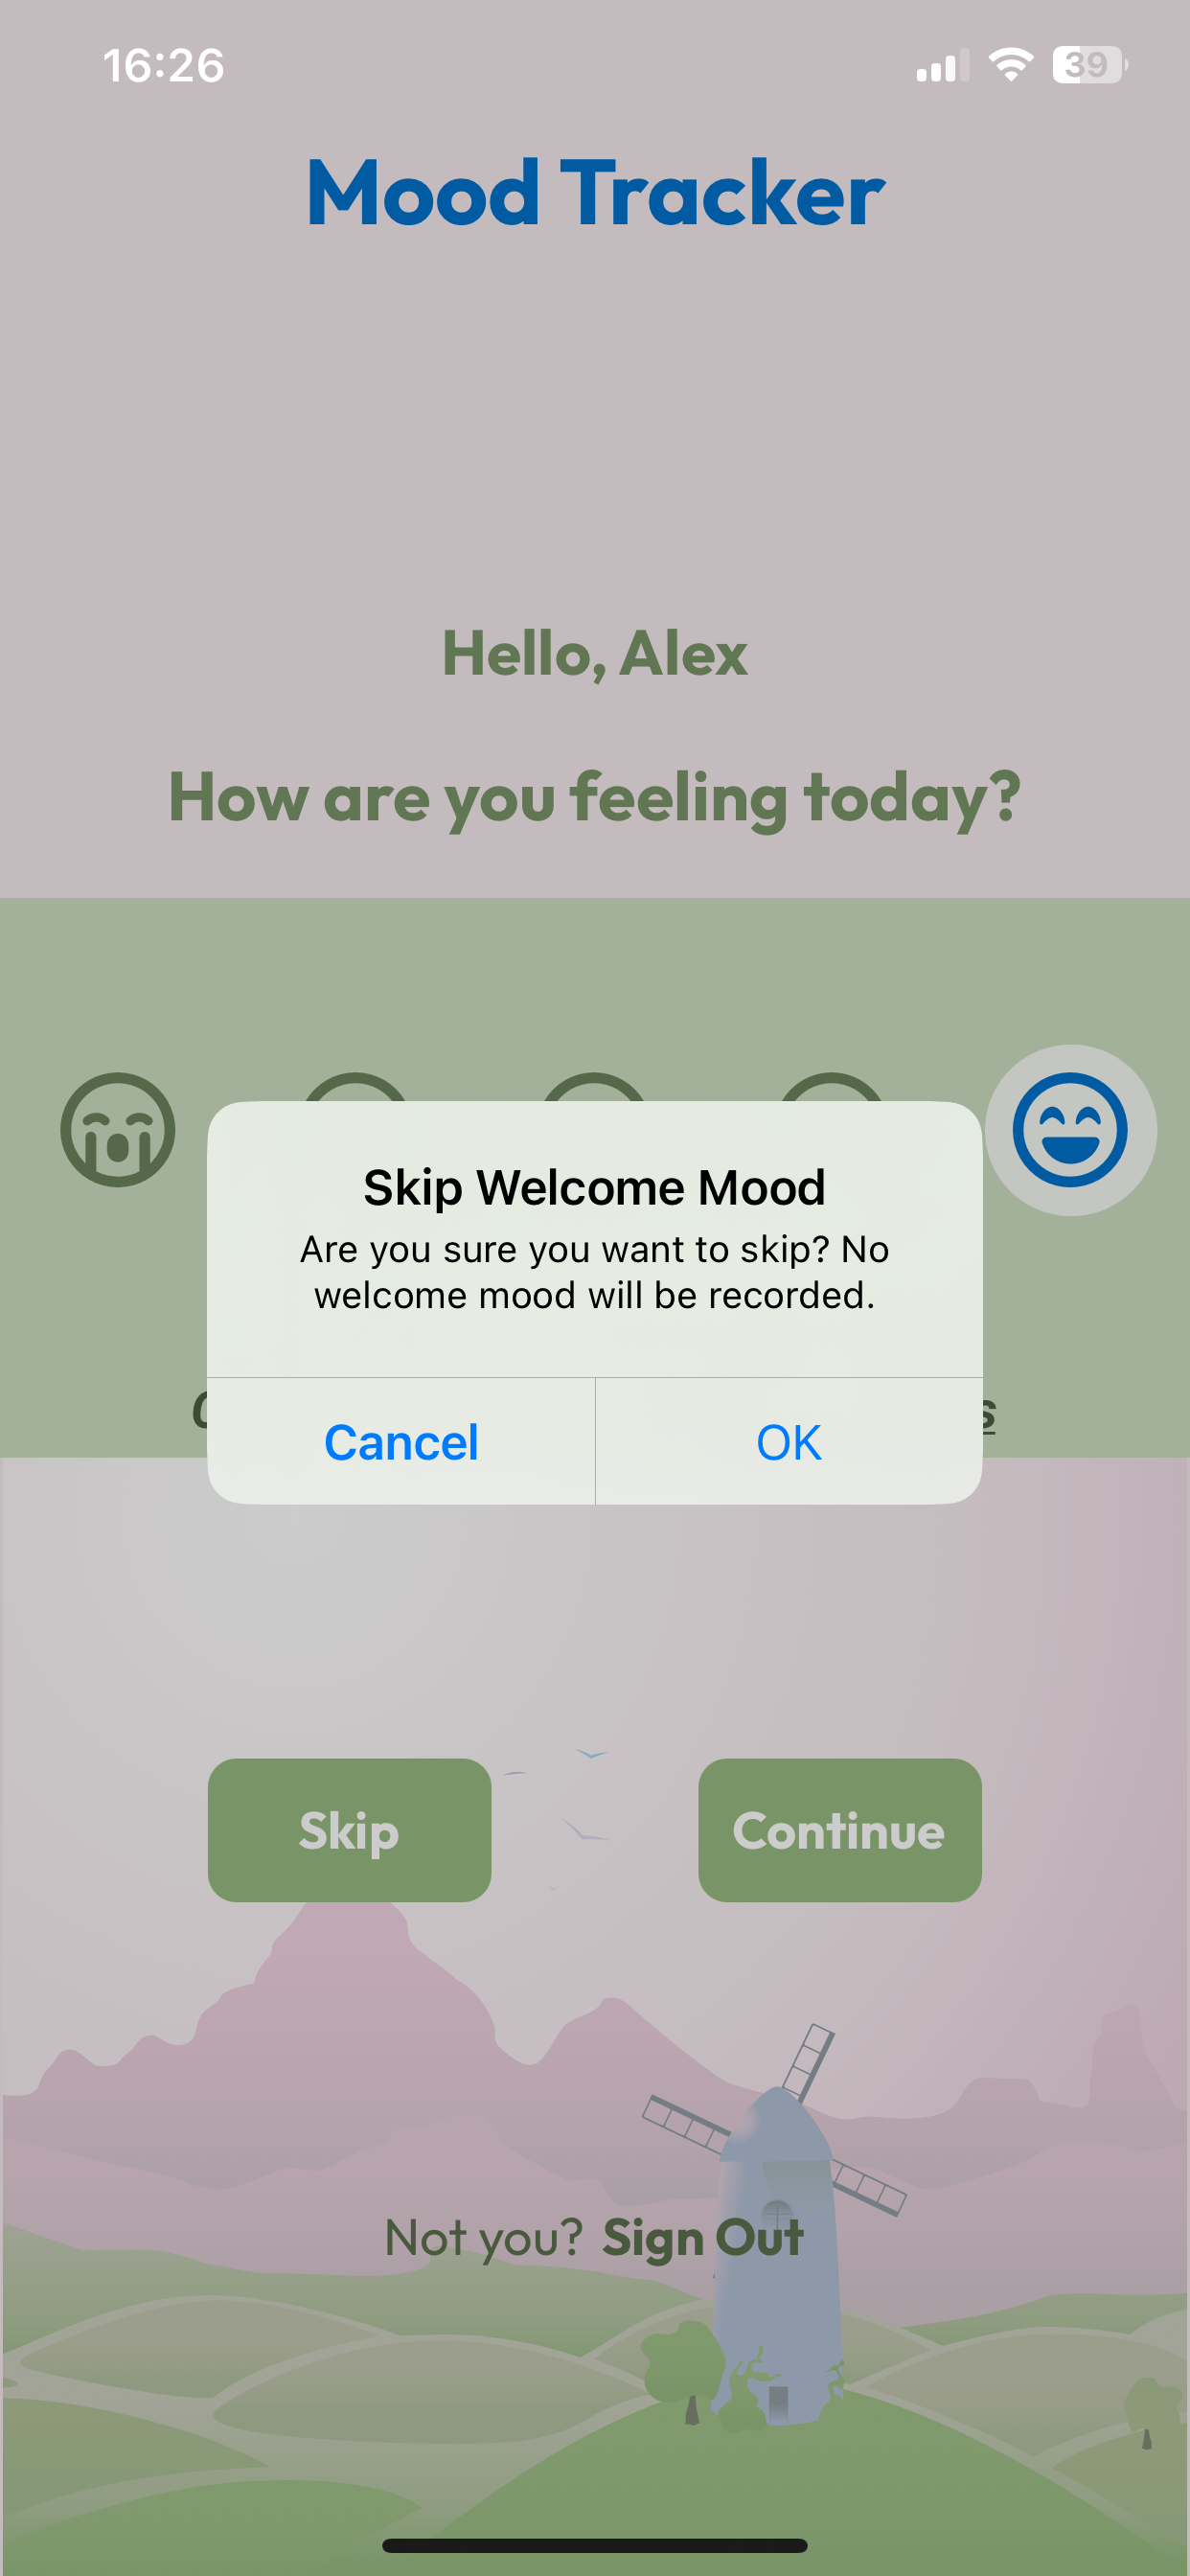
\includegraphics[scale=0.11]{figures/screenshots/Welcome Screen/7.PNG}\label{fig:skip-procedure}}
    \caption{Welcome Screen functionalities}
\end{figure}
\FloatBarrier

\vspace{5mm}

\subsection{Home Screen}

The Home Screen is the main dashboard of the application, providing a comprehensive overview of the user's mood history, motivational content, and other key features. The screen is personalized with a greeting like ``Hello, Alexandros'' (or the user's name respectively), along with a profile picture and the streak of consecutive days the user has been active. Also an icon is shown, which changes depending on if the user has completed today's survey.\vspace{5mm} \\
At the top of the screen, a ``Quote of the Day'' or ``Advice'' section is displayed, containing motivational quotes or helpful messages based on the user’s mood data. Below this section, there is a ``Welcome Moods of the week'' area, which visualizes the user’s mood for each day of the current week using a color-coded system that represents the emotional states such as ``Awful,'' ``Sad,'' ``Neutral,'' ``Good,'' and ``Happy.'' Users can easily see how their mood has changed over the week.\vspace{5mm} \\
The lower portion of the screen shows a ``Last 10 Questionnaires'' graph, which displays the distribution of the user’s responses over the past 10 questionnaires using a pie chart. This helps users to quickly understand their emotional trends and overall mental state.\vspace{5mm} \\
Navigation buttons at the bottom allow users to switch between different sections of the app, such as the ``Home'' screen and the ``Questionnaires'' screen,

\vspace{5mm}

\FloatBarrier
\begin{figure}[ht]
    \centering
    \subfloat[Home Screen]{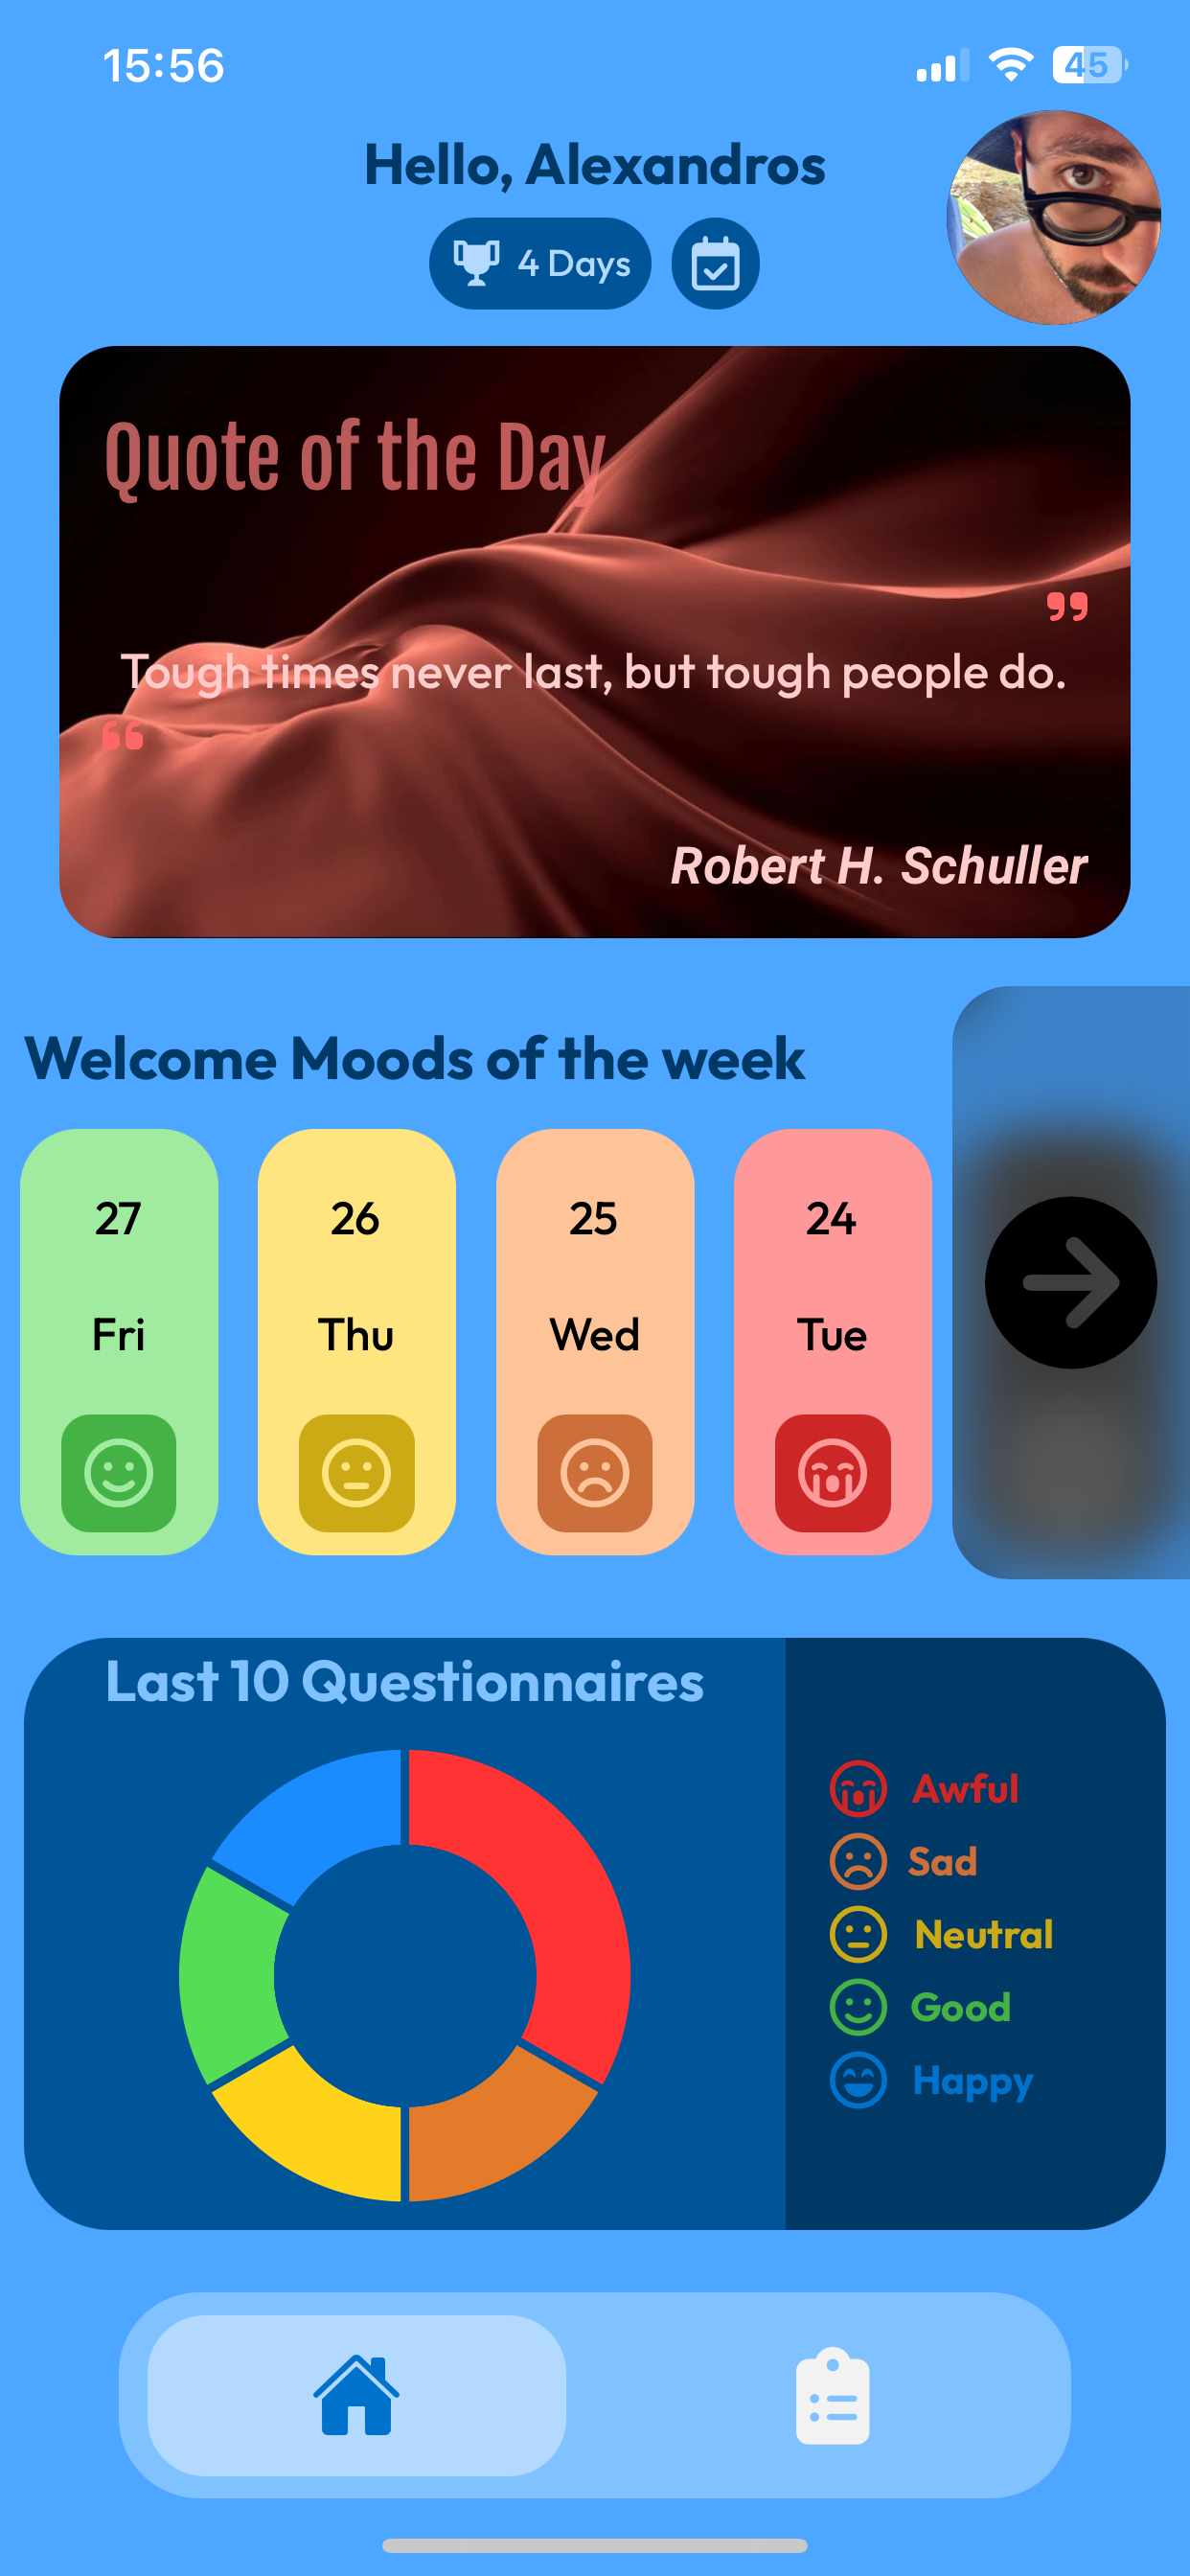
\includegraphics[scale=0.12]{figures/screenshots/Home - Calendar - Graph/1.PNG}\label{fig:home-page}}
    \hspace{10mm}
    \subfloat[New Message]{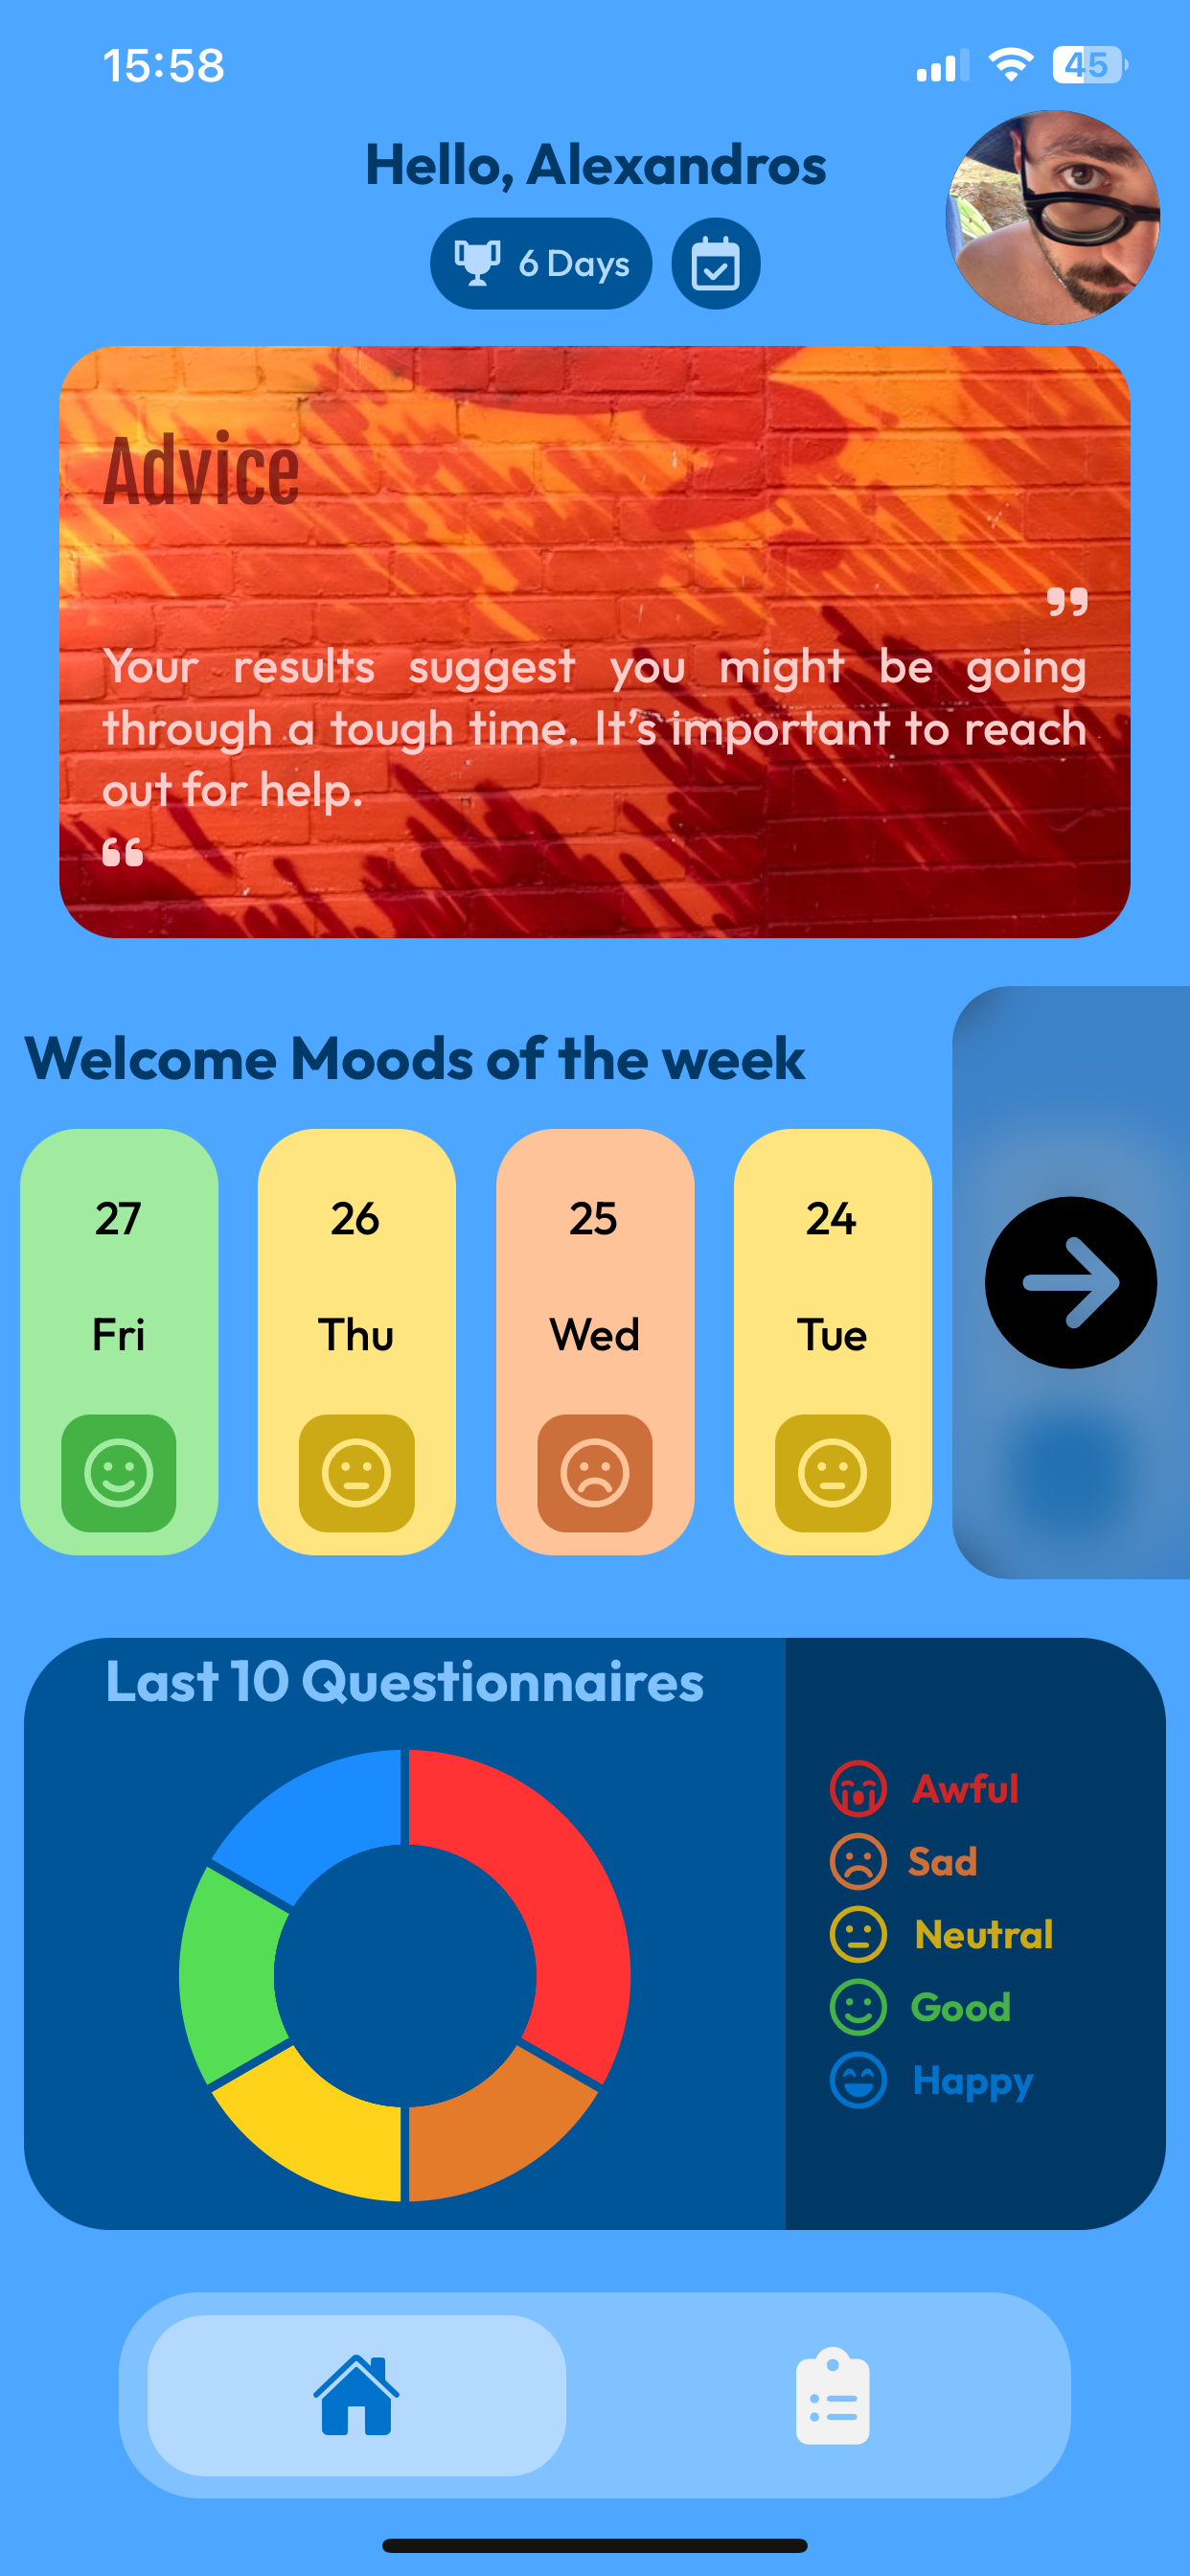
\includegraphics[scale=0.12]{figures/screenshots/Home - Calendar - Graph/6.PNG}\label{fig:new-message}}
    \caption{Home Screen - Overview and New Message Notification}
\end{figure}
\FloatBarrier

\vspace{5mm}

\subsection{Questionnaires Screen}

\vspace{5mm}

The \textbf{Questionnaires Screen} serves as the main page for accessing the daily and previous surveys. Users can view a list of surveys they have participated in and check the duration it took to complete each one. This screen is divided into two main sections:

\begin{itemize}
    \item \textbf{Today's Survey}: This section displays the current survey that the user can take. The banner at the top highlights that a new survey is available, and the user can tap on it to begin answering the questions.
    \item \textbf{Previous Surveys}: This section provides a chronological view of the previously completed surveys, grouped by survey number and also by date. Each entry shows the day of the week and the completion time for that specific survey. Tapping on any of the previous surveys allows the user to view their responses.
\end{itemize}

\FloatBarrier
\begin{figure}[ht]
    \centering
    \subfloat[Questionnaires Screen]{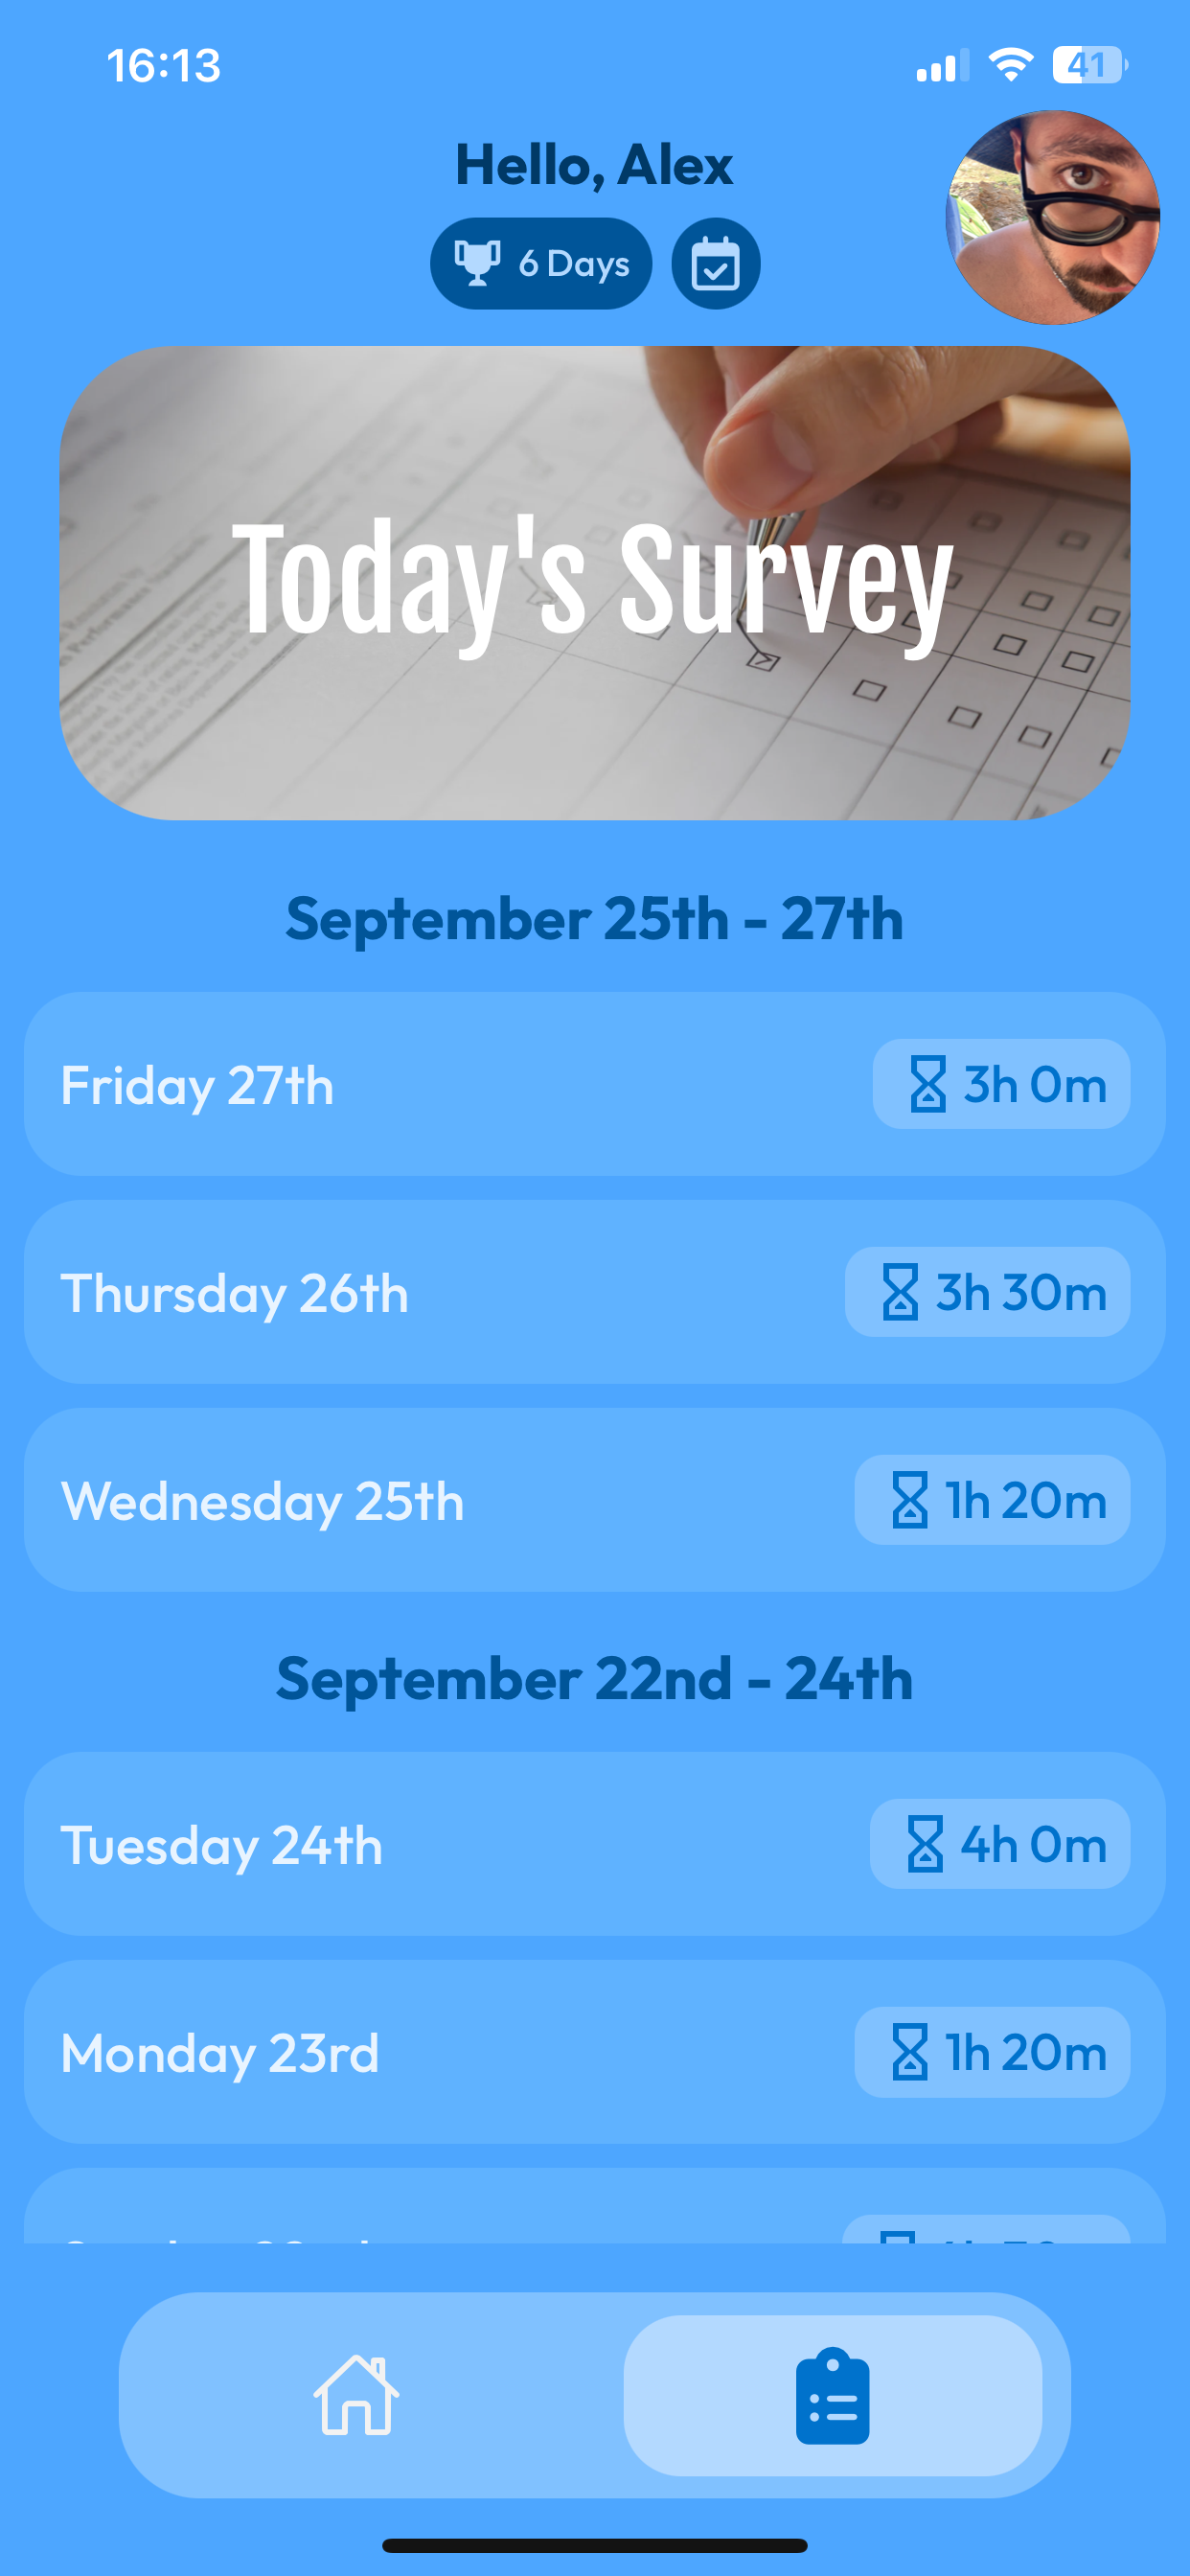
\includegraphics[scale=0.12]{figures/screenshots/Questionnaire - Survey/1.PNG}\label{fig:questionnaires-page}}
    \hspace{10mm}
    \subfloat[Previous surveys]{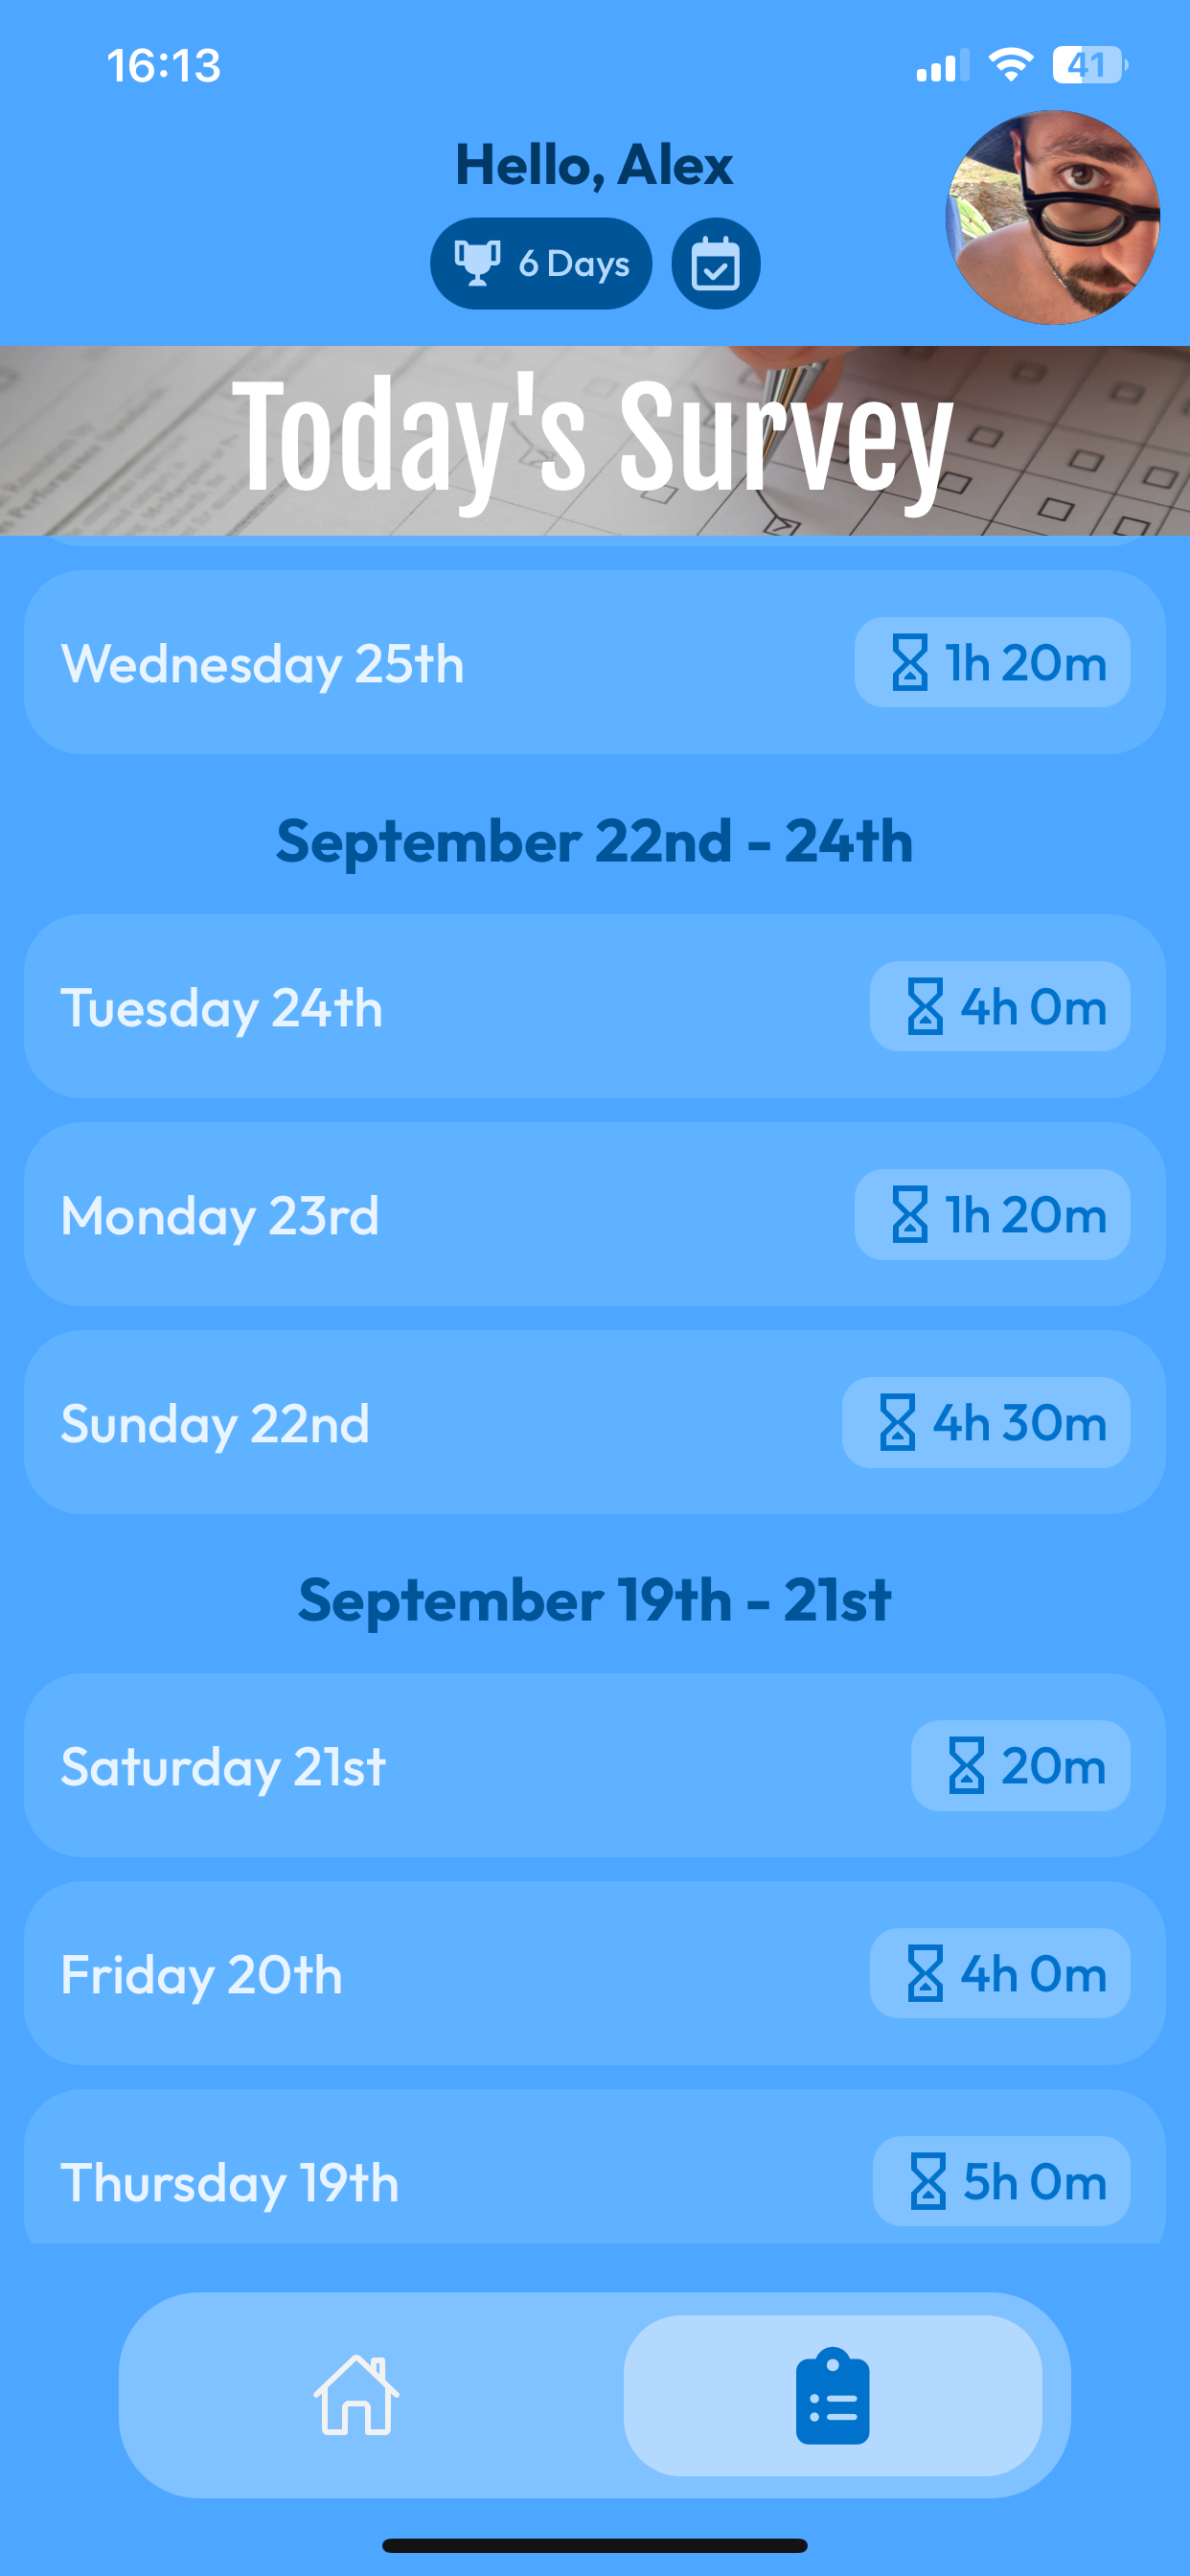
\includegraphics[scale=0.12]{figures/screenshots/Questionnaire - Survey/2.PNG}\label{fig:questionnaires-more-previous-surveys}}
    \caption{Procedure - View previous survey questionnaires}
\end{figure}
\FloatBarrier

\vspace{5mm}

\subsection{Previous Survey}

The Previous Survey screen highlights how a user can review their responses to questions in previously taken surveys. This functionality allows the user to revisit past entries and reflect on how their emotions and thoughts have evolved over time. The user can also read through their comments and the options they chose for each question.\vspace{5mm} \\
The user can navigate between the questions using the ``Continue'' button on the bottom, or the left arrow on the top left corner of the screen, to get to the next or the previous questions respectively. If the wnat to exit the whole questionnaire, they can press the ``Exit'' button. They can also view the points that they gethered in this survey.

\vspace{5mm}

\FloatBarrier
\begin{figure}[ht]
    \centering
    \subfloat[Question 1]{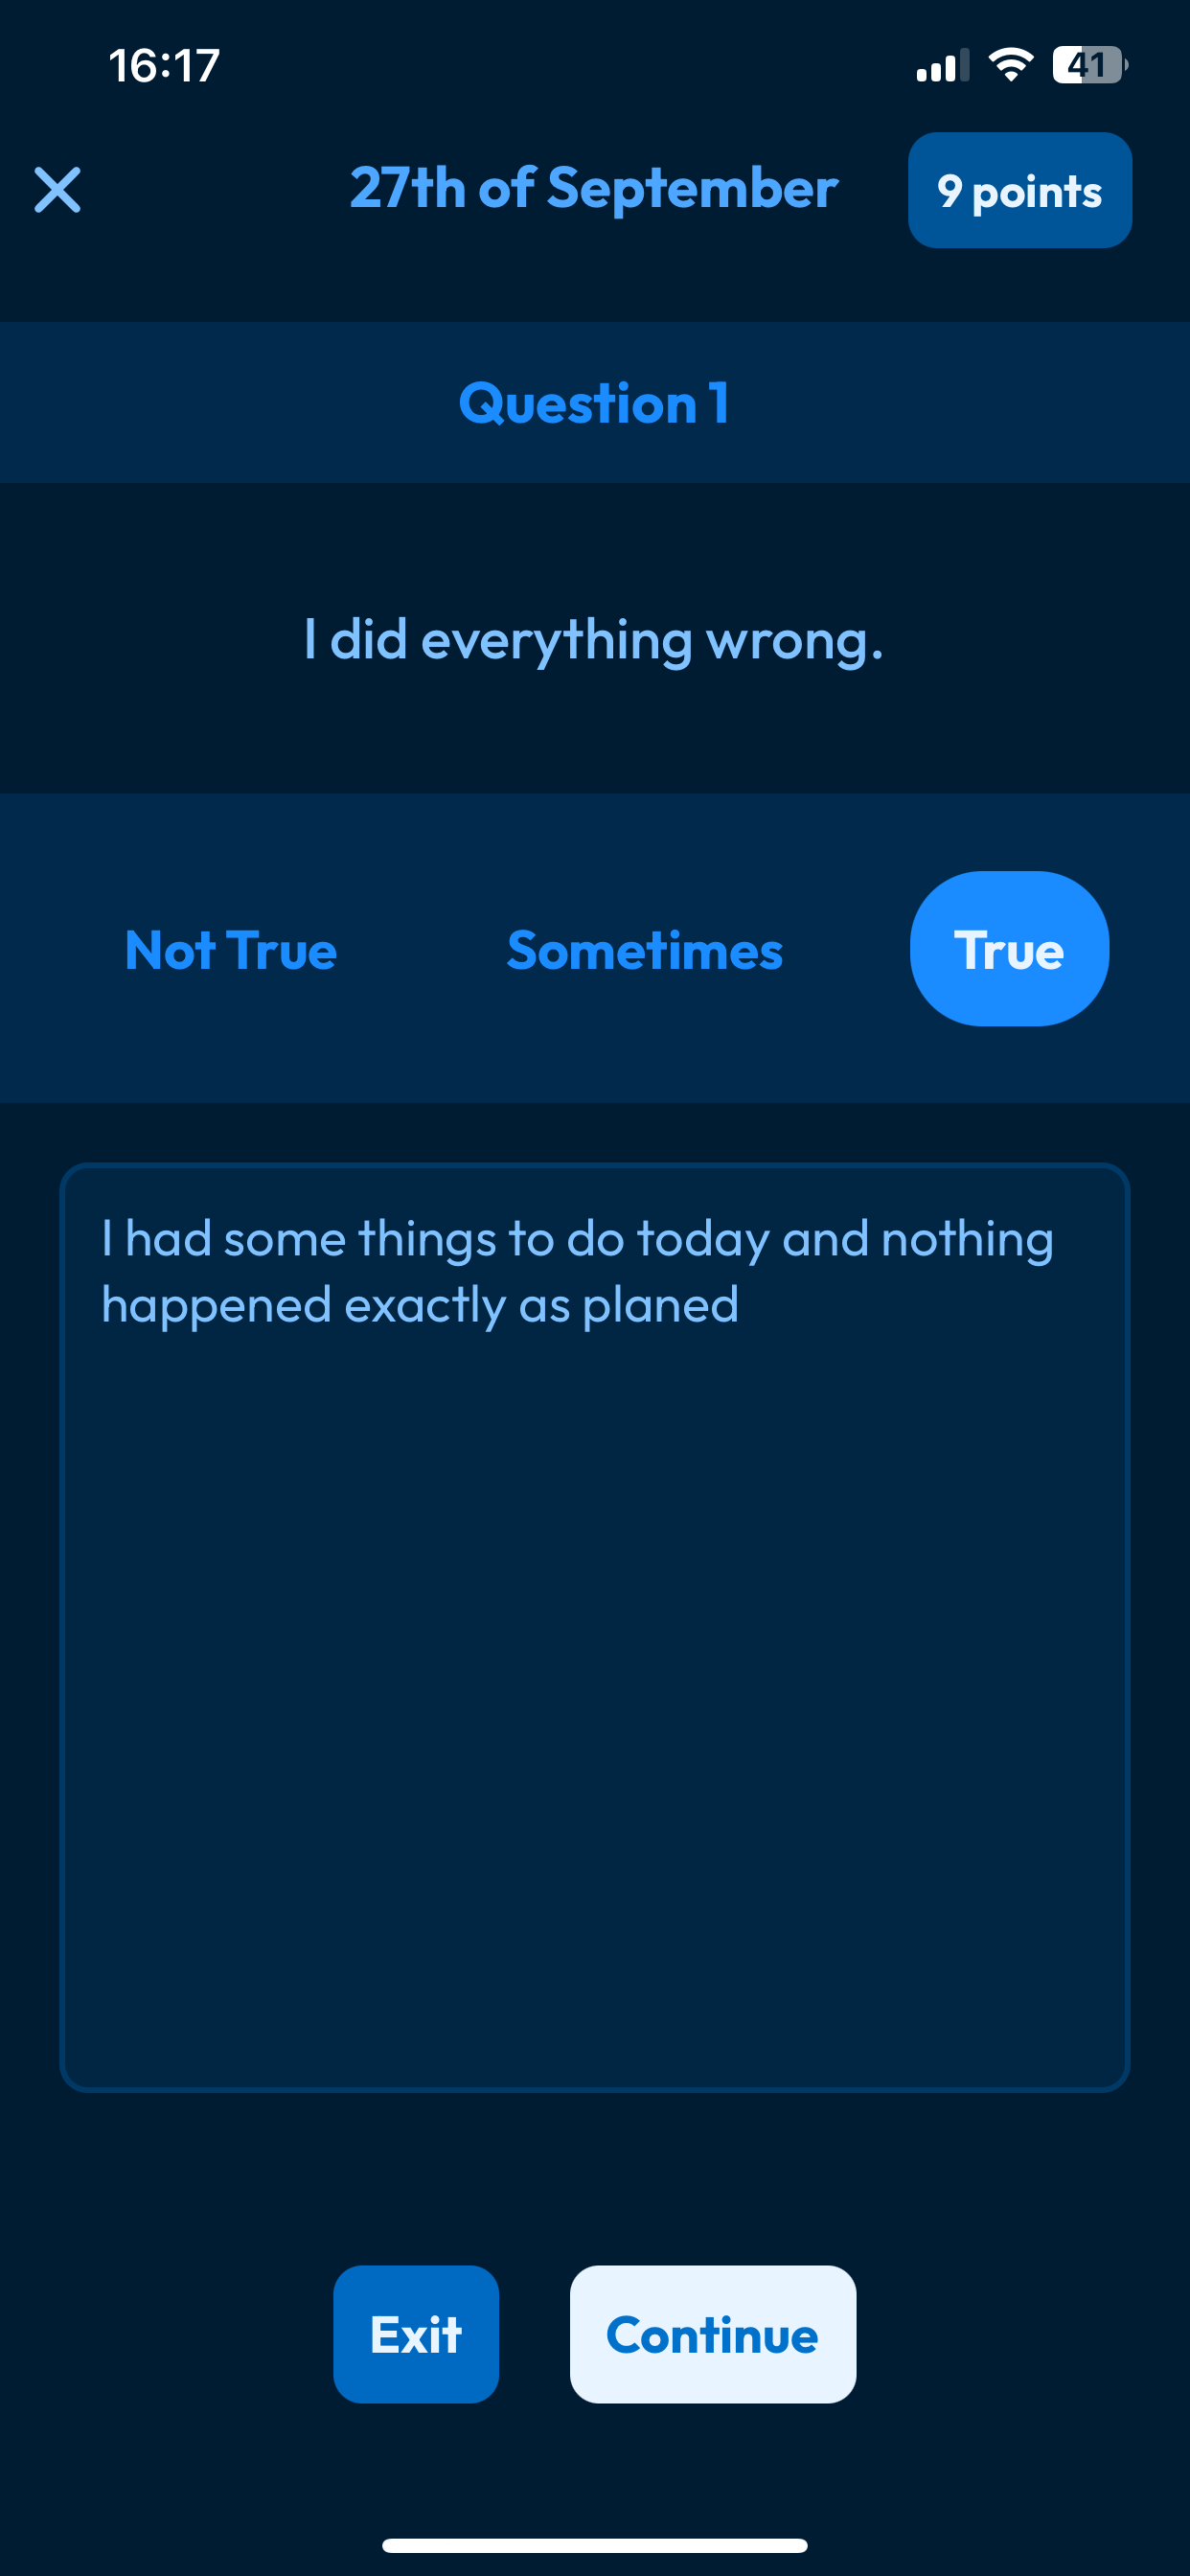
\includegraphics[scale=0.12]{figures/screenshots/Questionnaire - Survey/3.PNG}\label{fig:previous-survey-question-1}}
    \hspace{10mm}
    \subfloat[Question 2]{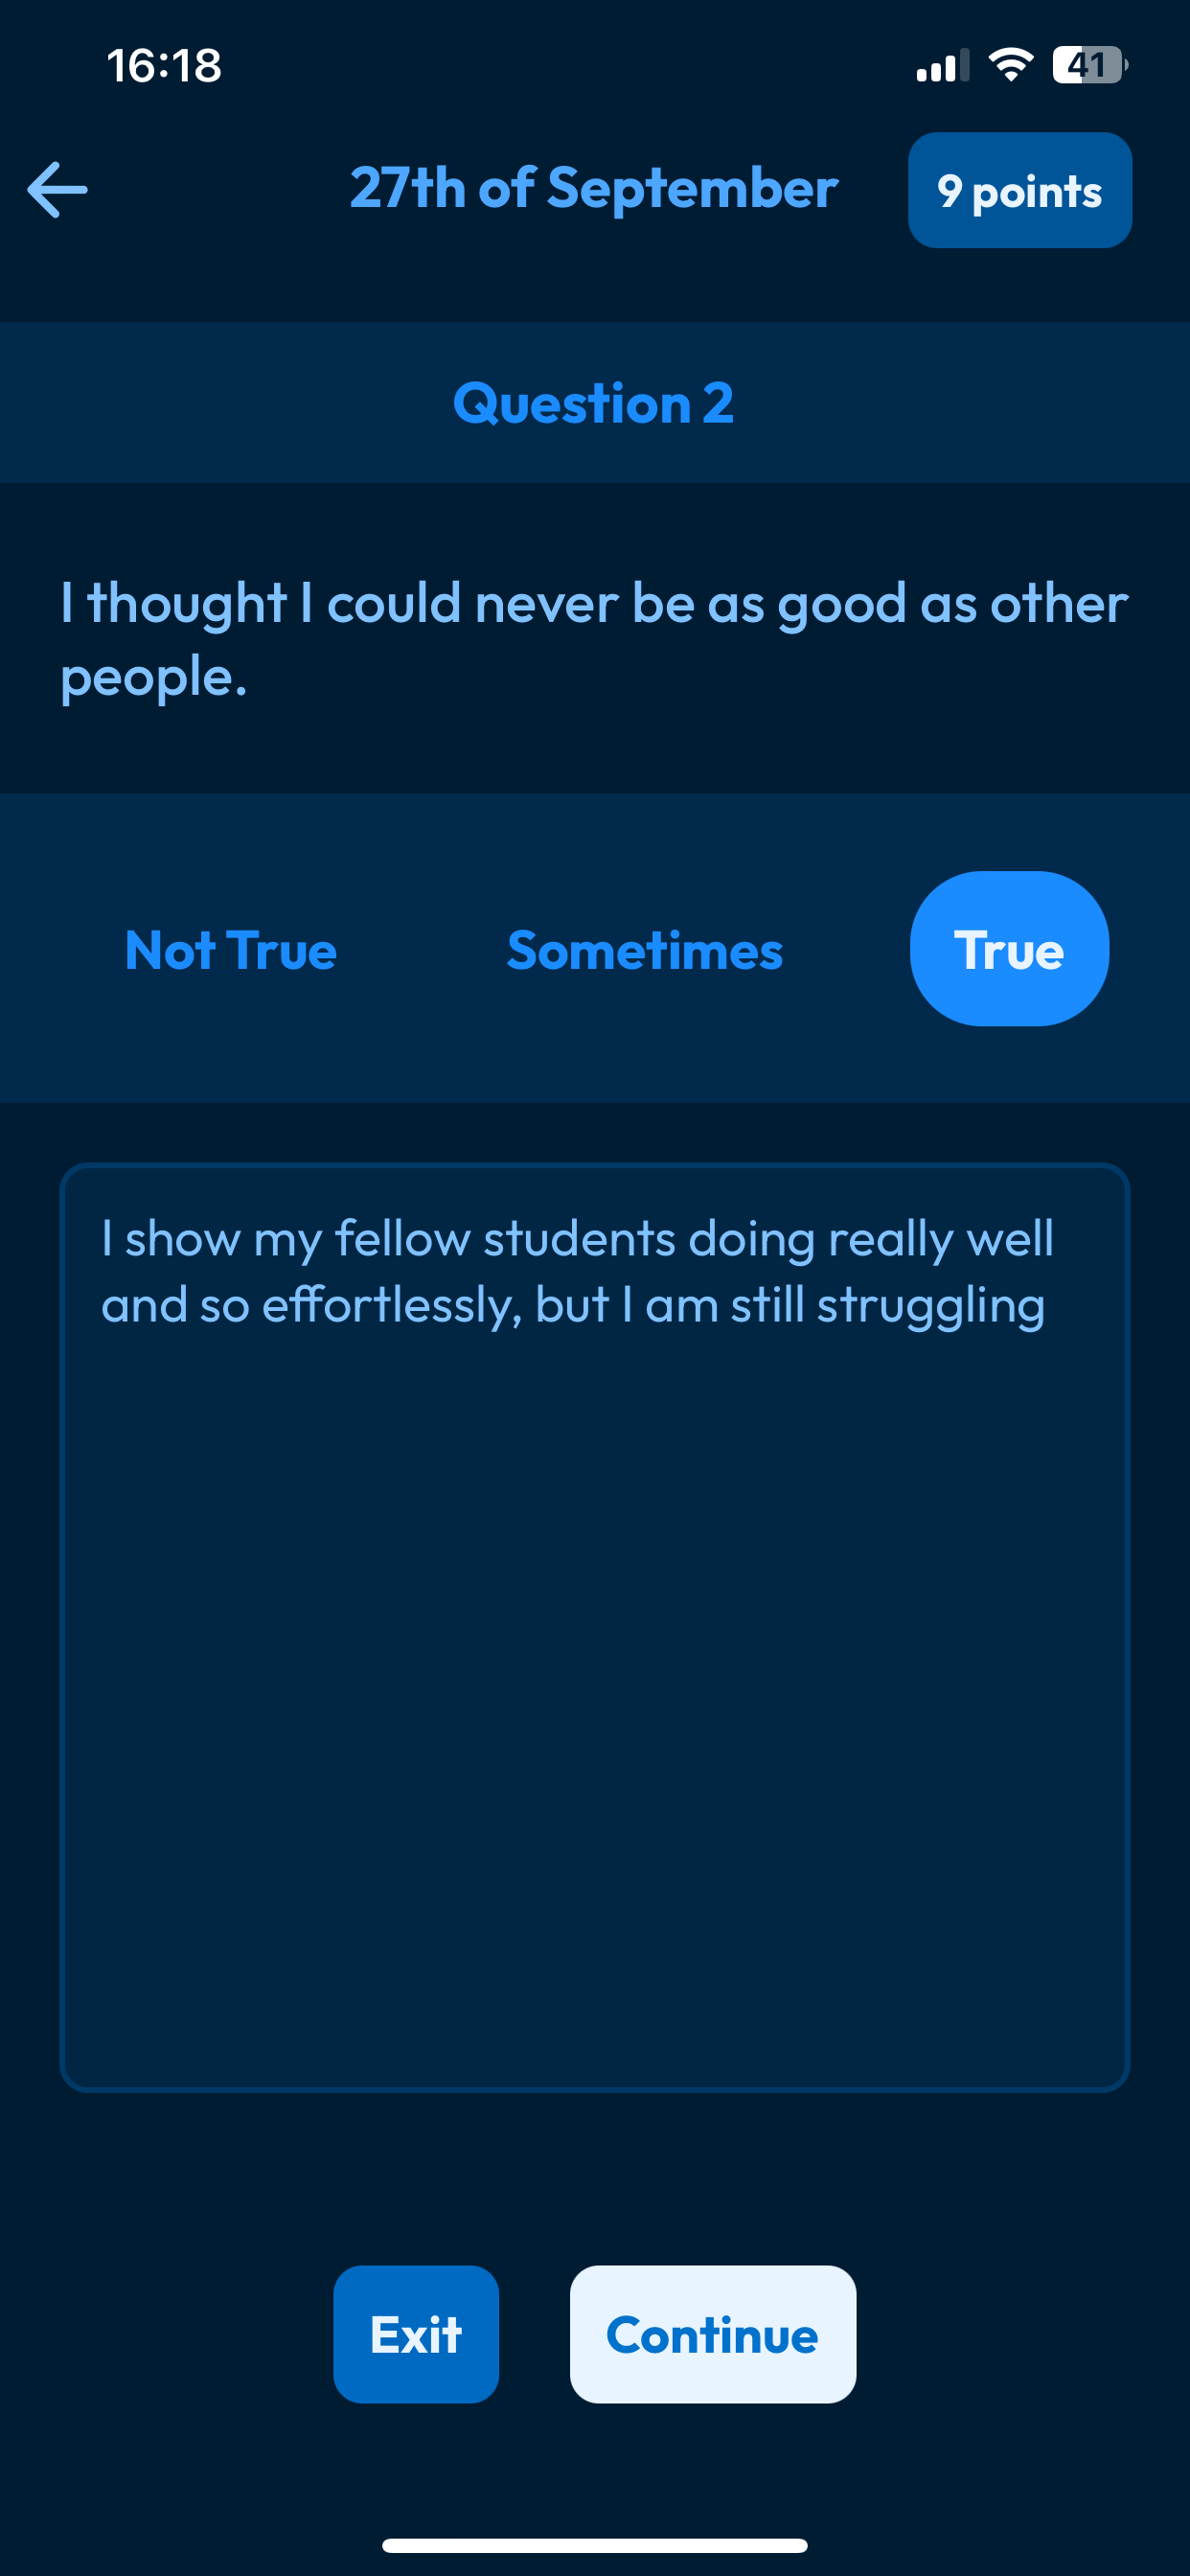
\includegraphics[scale=0.12]{figures/screenshots/Questionnaire - Survey/4.PNG}\label{fig:previous-survey-question-2}}
    \caption{Review of a previous survey with multiple questions}
\end{figure}
\FloatBarrier

\vspace{5mm}

\subsection{Today's Survey}

The Today's Survey screen walks through the steps required to complete a survey for the current day. It provides an intuitive flow, guiding the user from the beginning of the survey to its completion. This screen includes a series of questions with predefined response options such as “Not True”, “Sometimes”, or “True”, along with an additional text box for the user to elaborate on their answers if desired. As soon as they answer a question, they can navigate to the next question using the ``Continue'' button. They can also go back to the previous question using the left arrow show on the top left corner of the screen. In the end, they complete the last question, and by pressing the ``Submit'' button, they can submit their survey responses.

\vspace{5mm}

\FloatBarrier
\begin{figure}[ht]
    \centering
    \subfloat[Step 1 - Answering a Question]{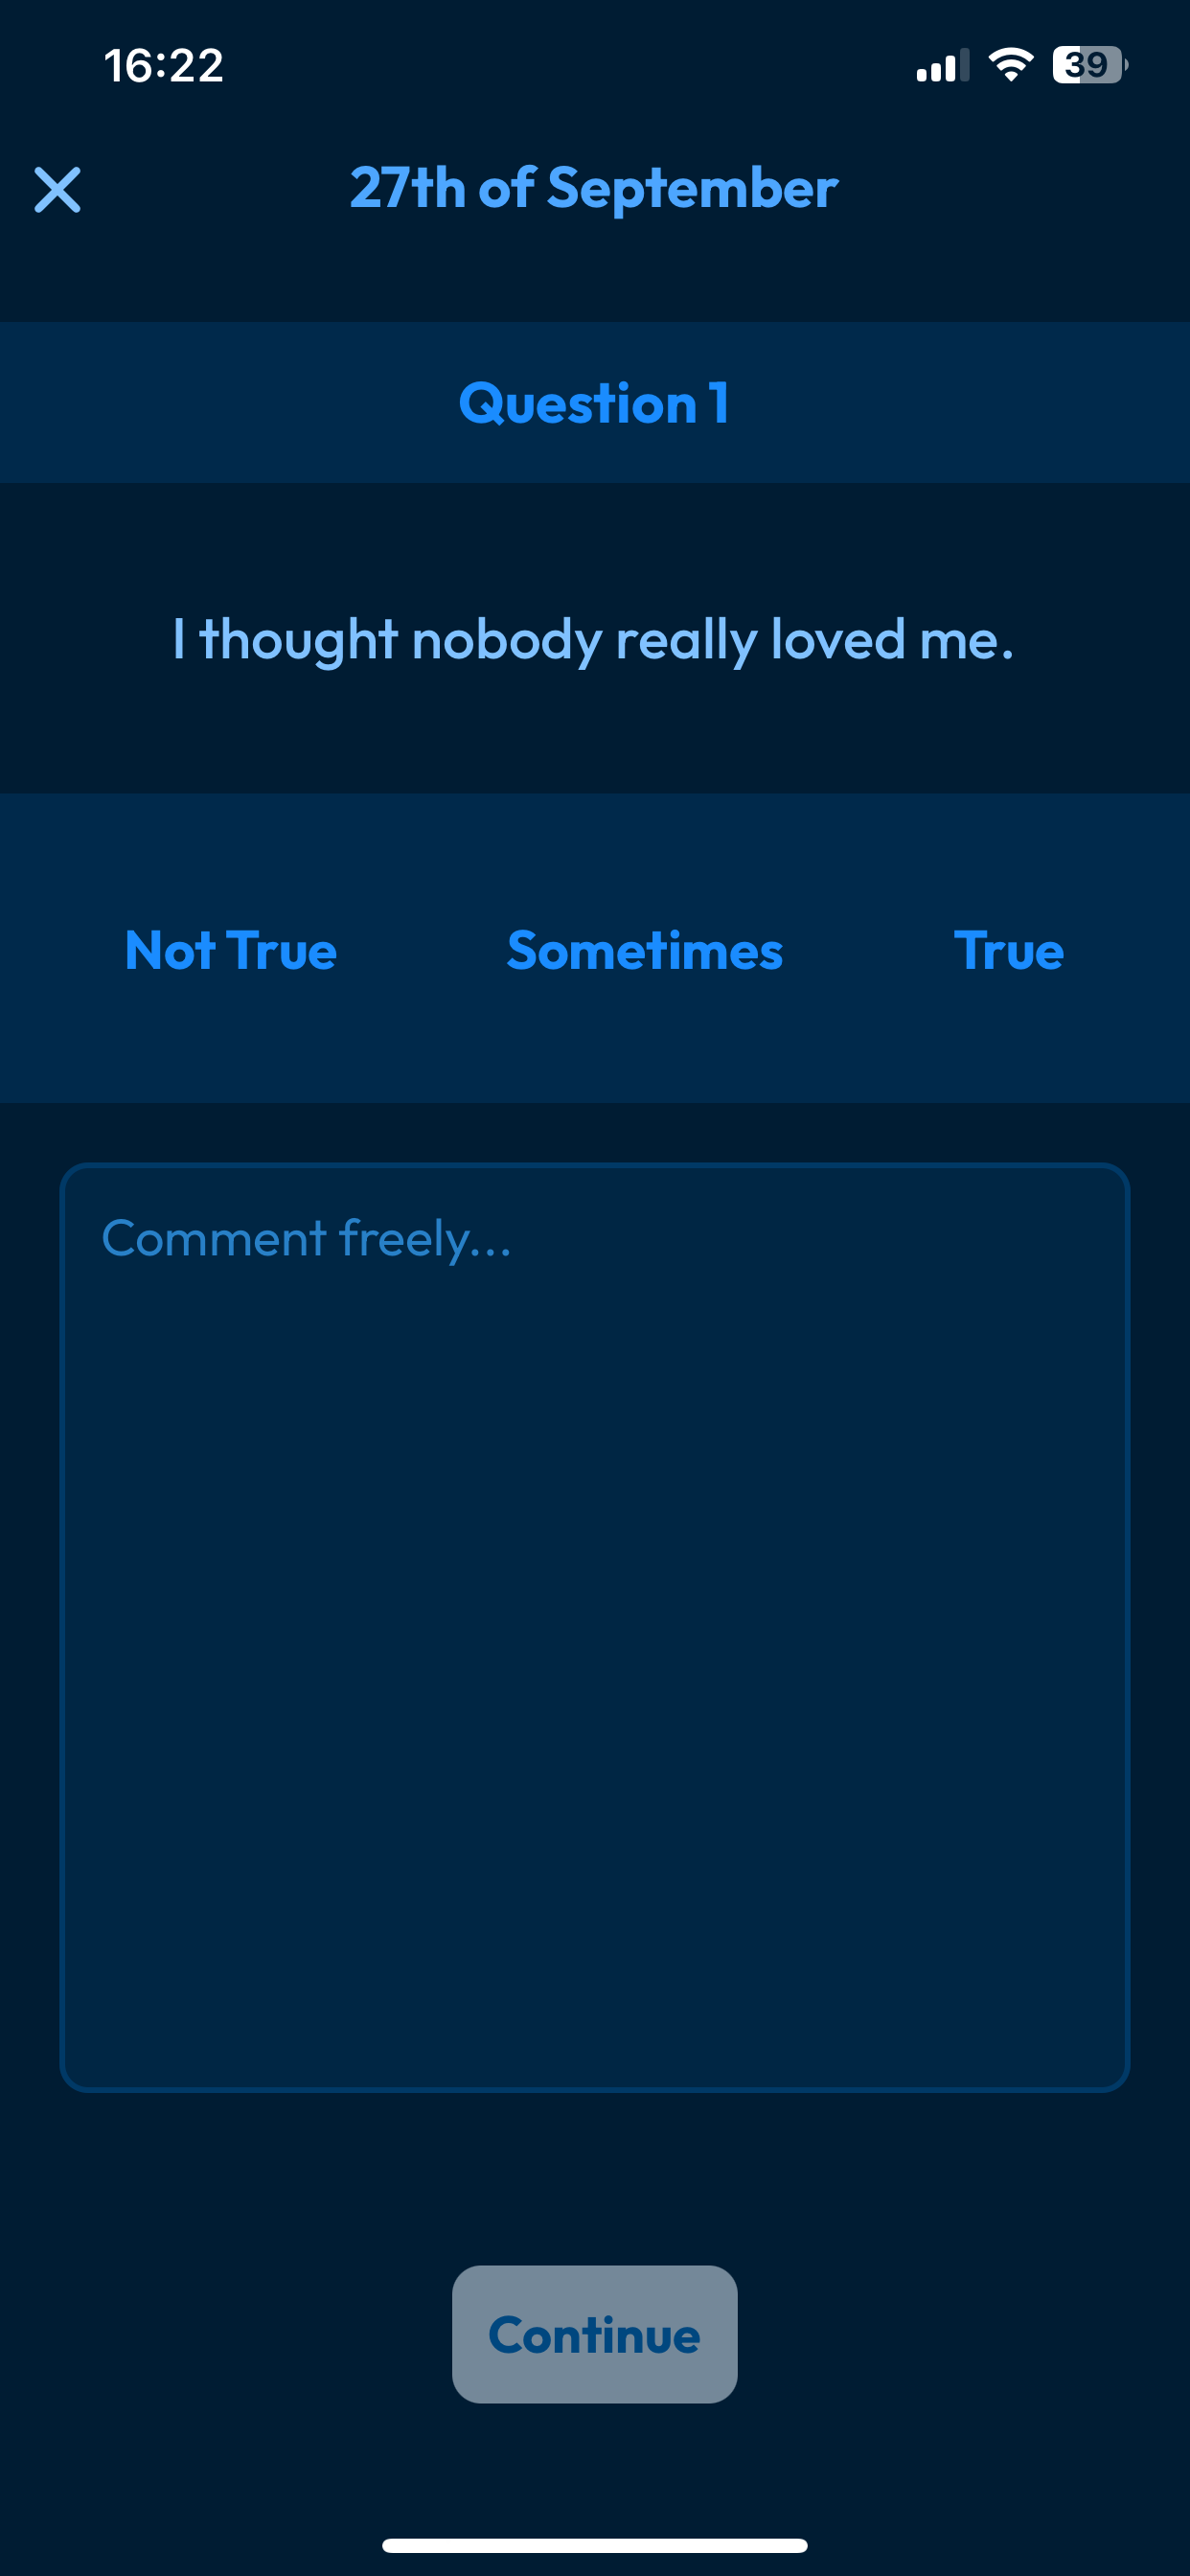
\includegraphics[scale=0.11]{figures/screenshots/Questionnaire - Survey/5.PNG}\label{fig:todays-survey-step-1}}
    \hfill
    \subfloat[Step 2 - Progress to Next Question]{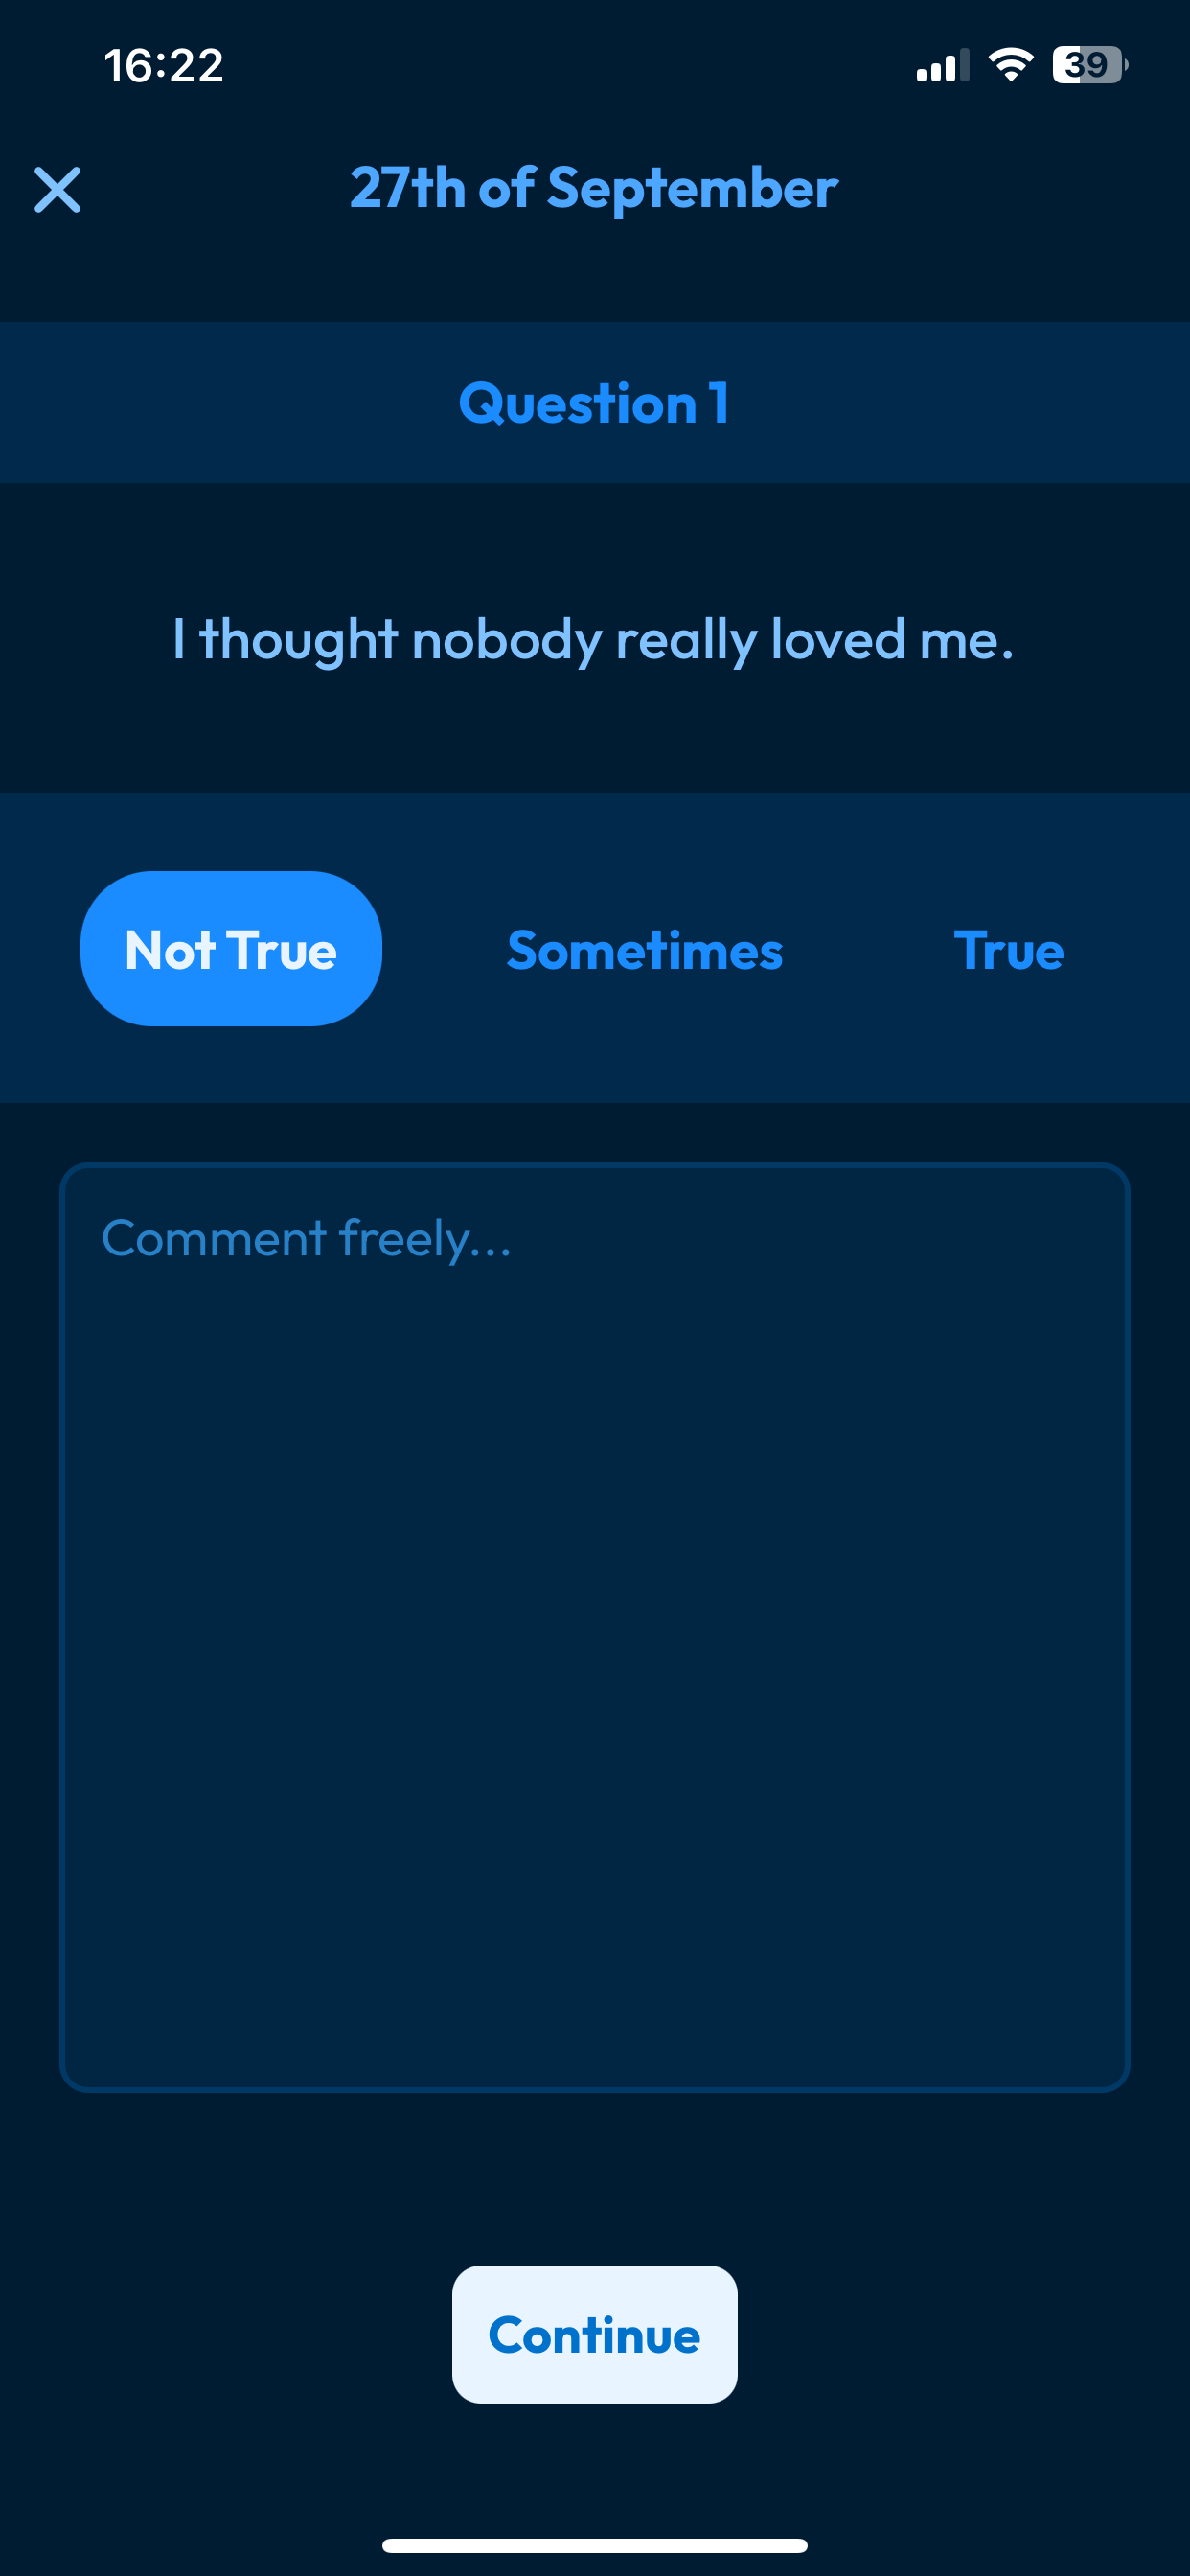
\includegraphics[scale=0.11]{figures/screenshots/Questionnaire - Survey/6.PNG}\label{fig:todays-survey-step-2}}
    \hfill
    \subfloat[Step 3 - Further Elaboration]{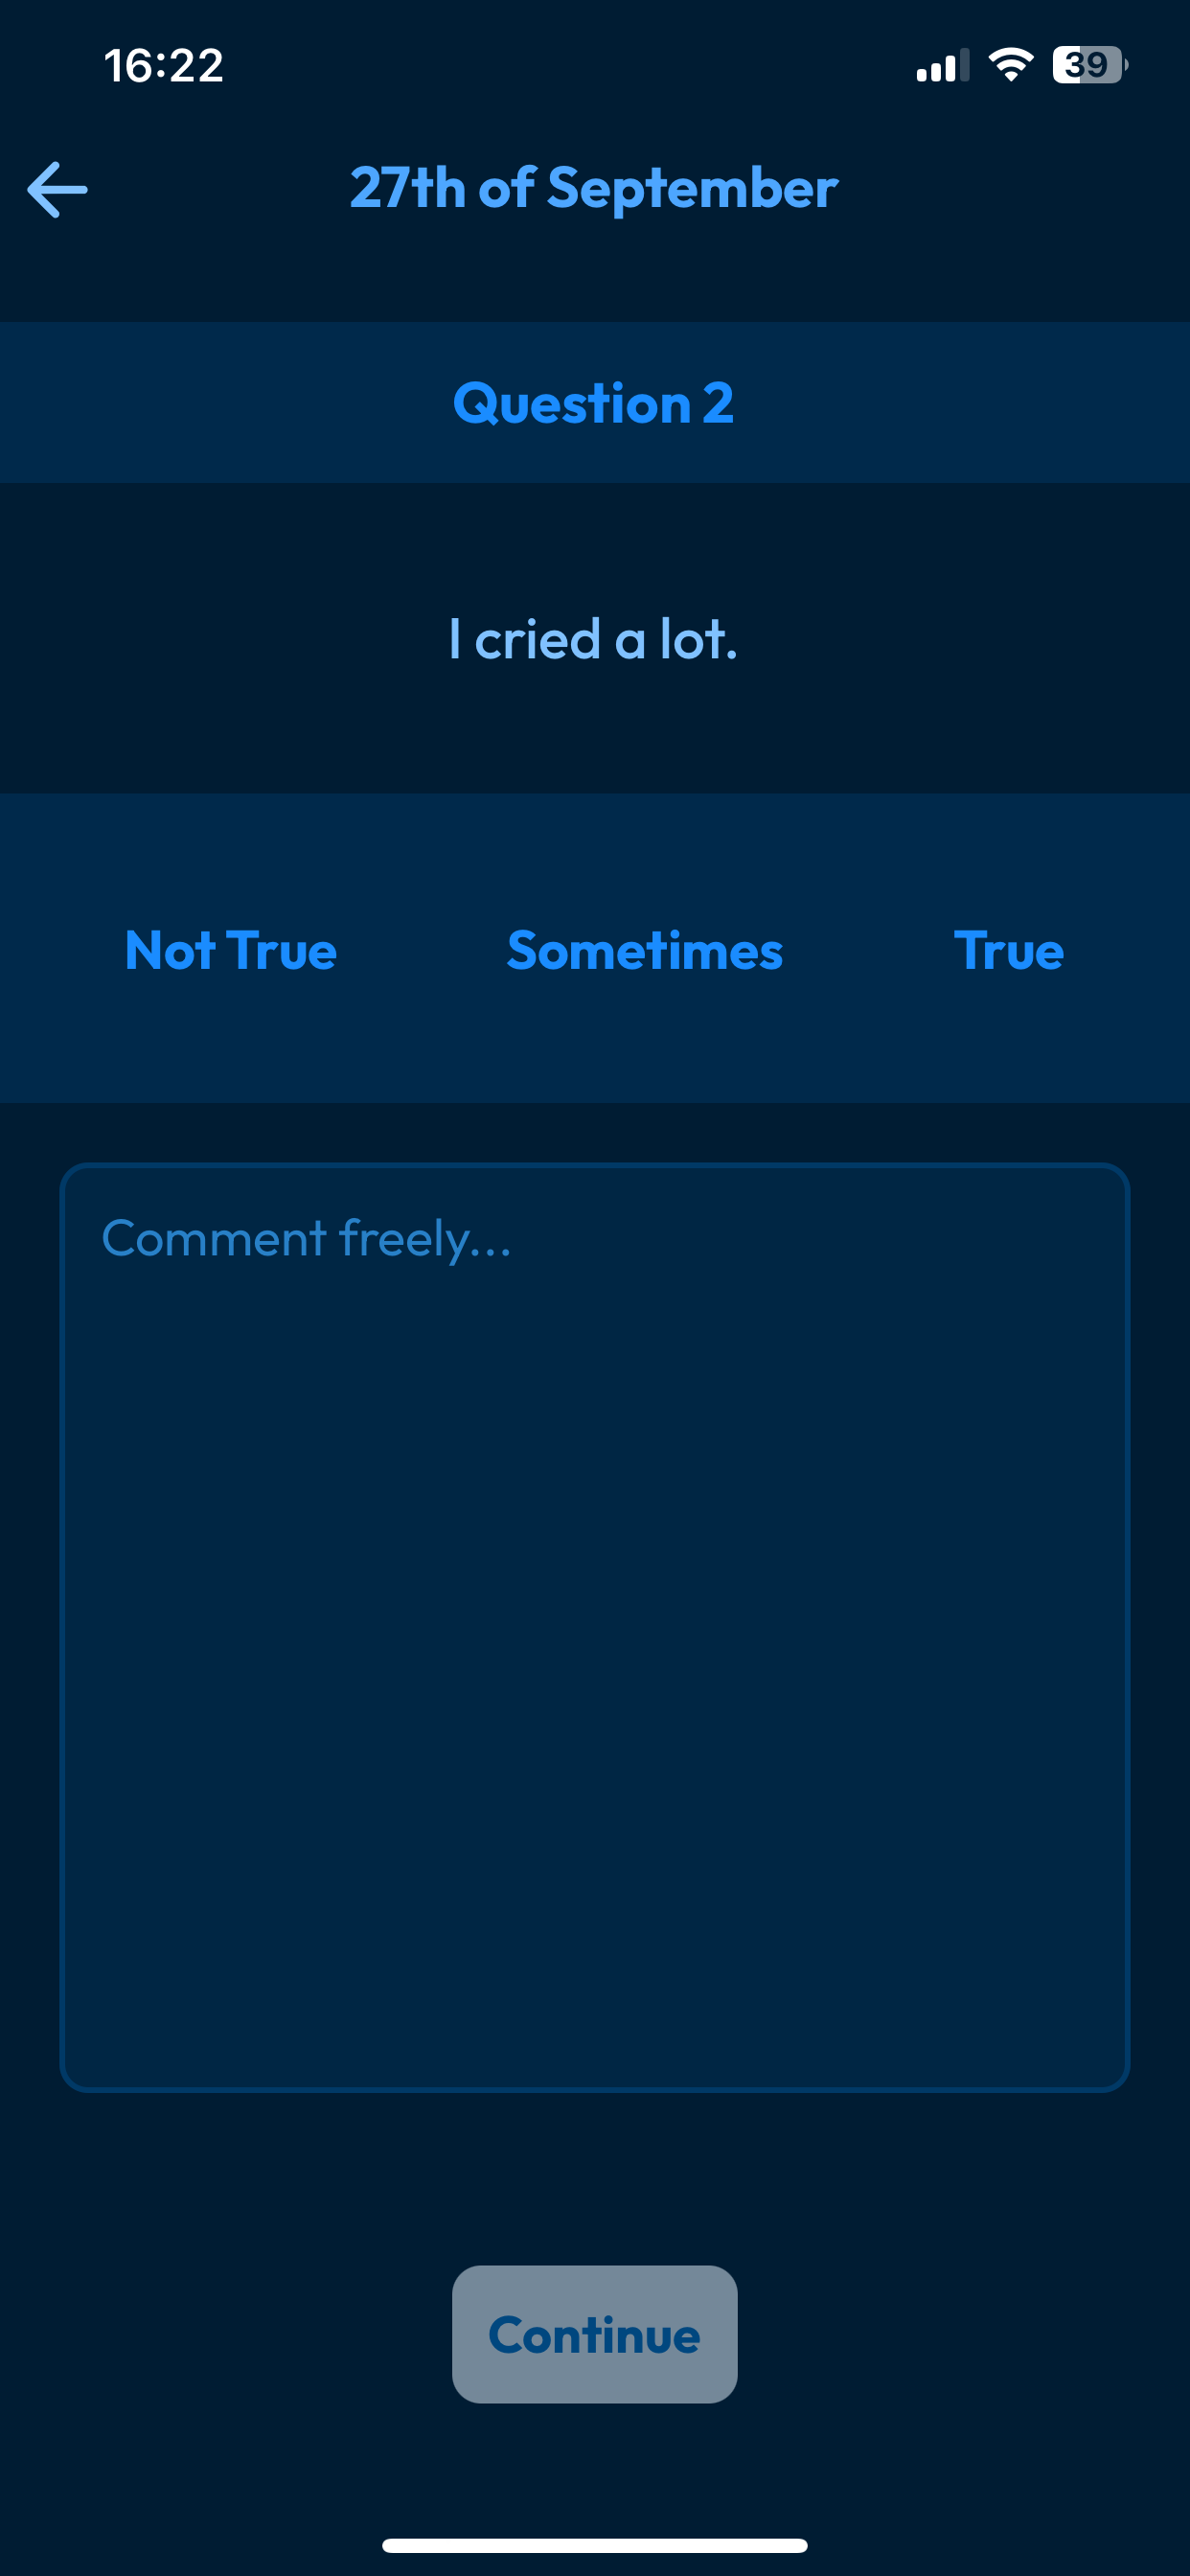
\includegraphics[scale=0.11]{figures/screenshots/Questionnaire - Survey/7.PNG}\label{fig:todays-survey-step-3}}
\end{figure}
\FloatBarrier

\vspace{5mm}

\FloatBarrier
\begin{figure}[ht]\ContinuedFloat
    \centering
    \subfloat[Step 4 - Submit Final Question]{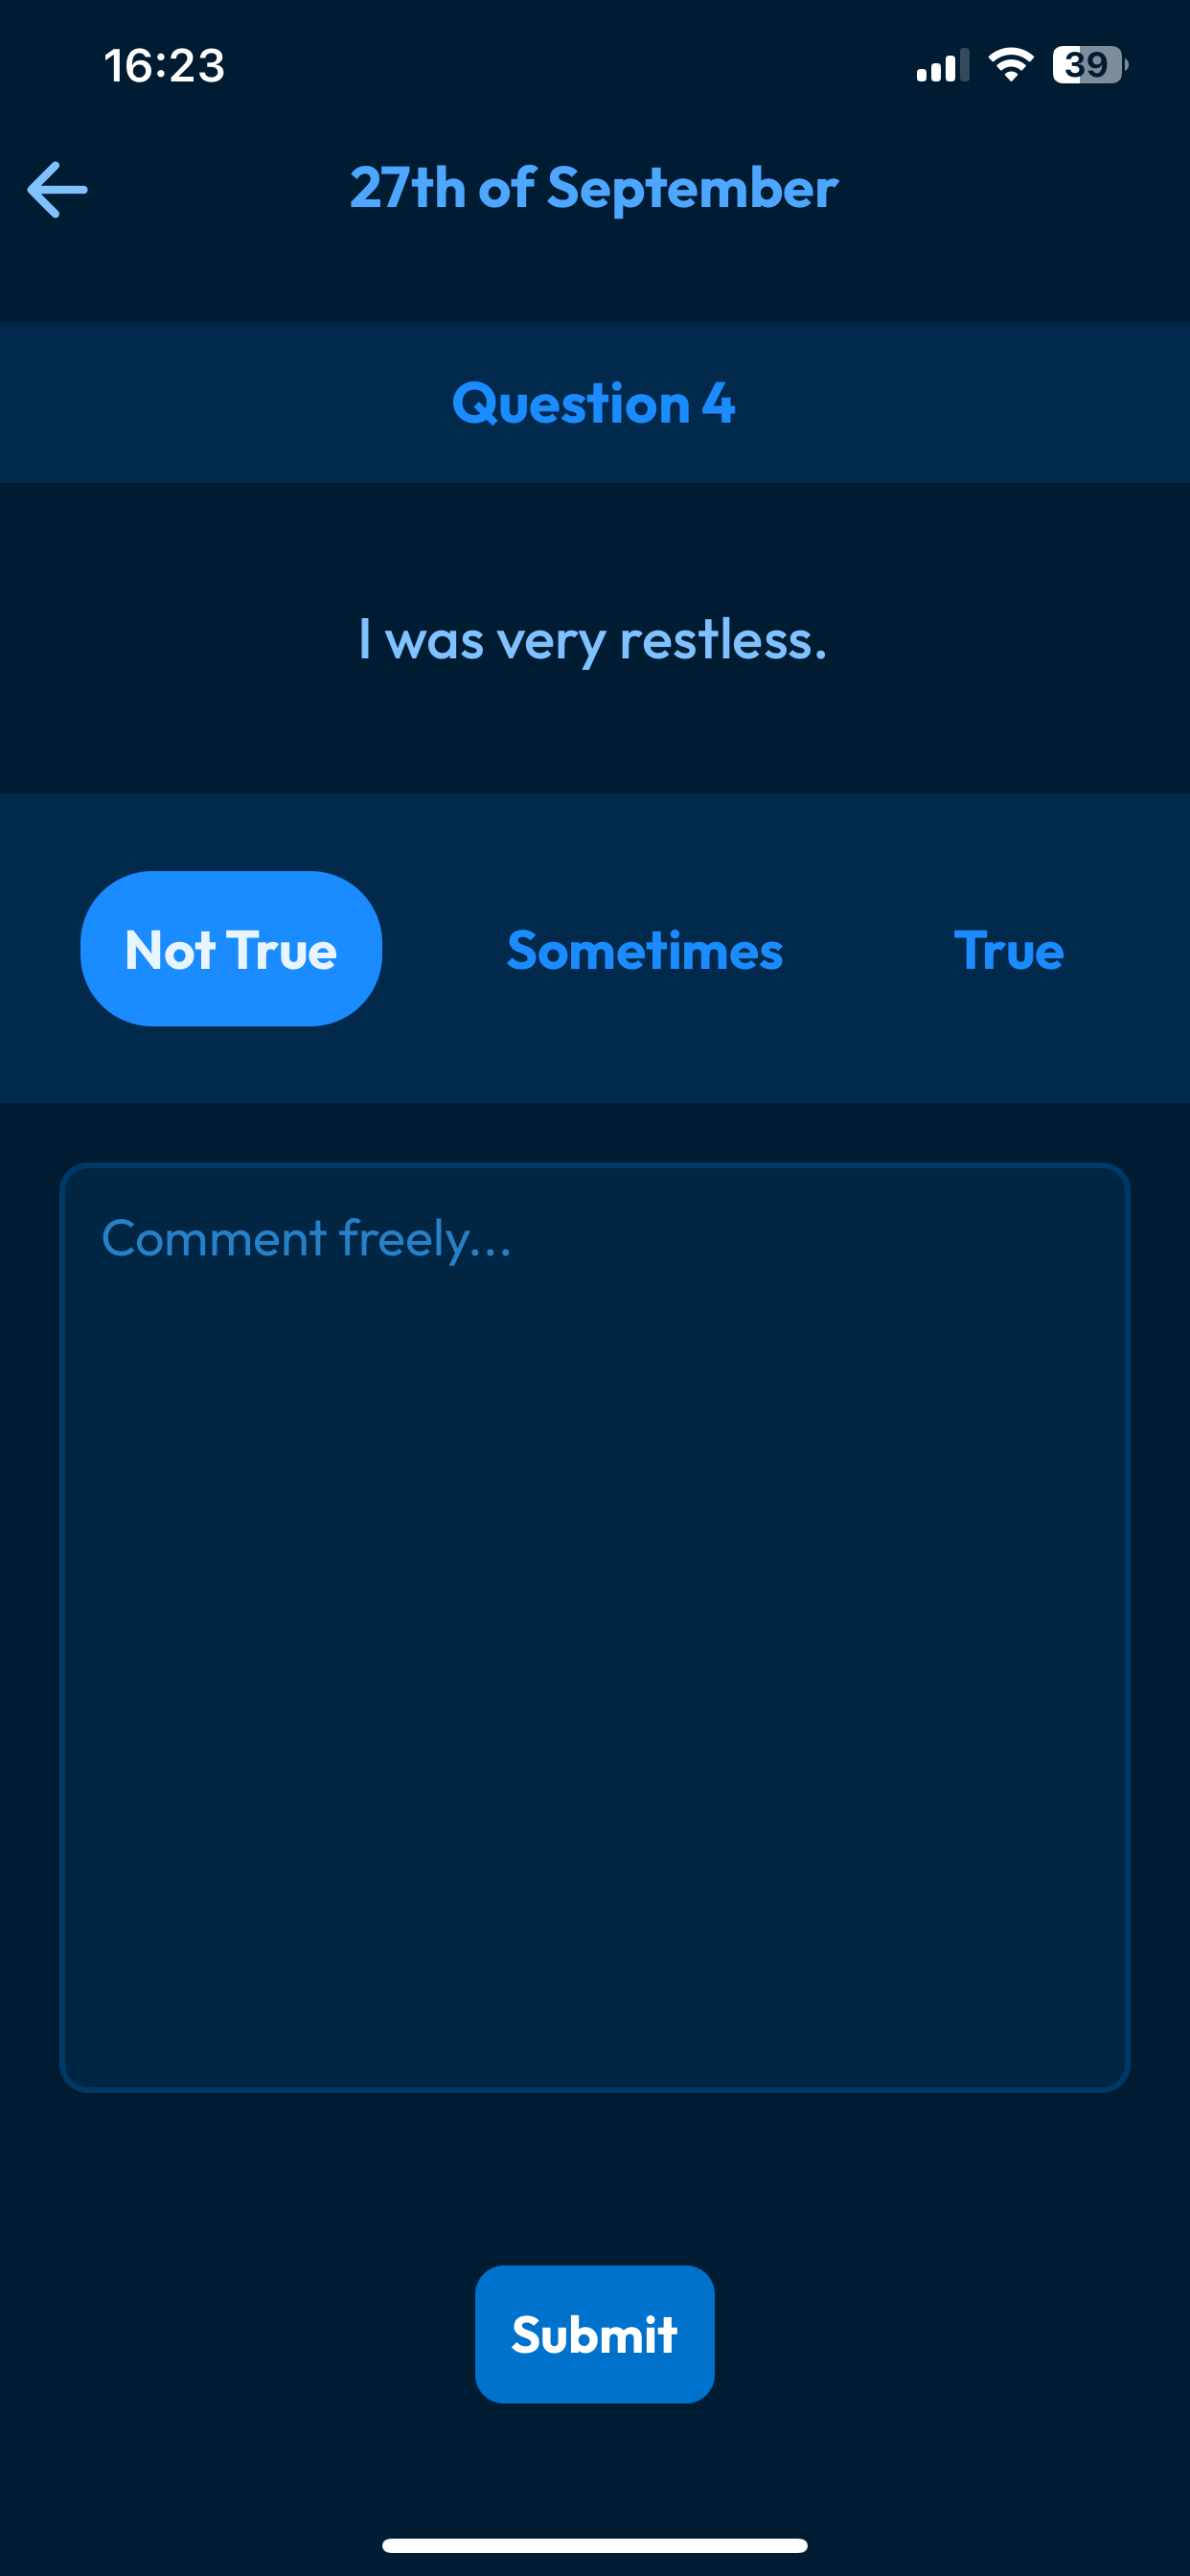
\includegraphics[scale=0.11]{figures/screenshots/Questionnaire - Survey/8.PNG}\label{fig:todays-survey-step-4}}
    \hspace{10mm}
    \subfloat[Survey Completion]{
\includegraphics[scale=0.11]{figures/screenshots/Questionnaire - Survey/9.PNG}\label{fig:todays-survey-completion}}
    \caption{Procedure - Complete today's survey}
\end{figure}
\FloatBarrier

\vspace{5mm}

\subsection{Calendar Screen}

The Calendar Screen provides an overview of the user's mood history for the entire month. Each day in the calendar is color-coded according to the user's recorded mood for that day. This visual representation allows users to quickly identify patterns and trends in their emotional states over the course of the month.\vspace{5mm} \\
Users can all tap on one of the six options below, each one of them assigned to one the different moods. This action shows the days during the month that the user had this welcome mood selected. Each option, contains the number of days right below its emoji.

\vspace{5mm}

\FloatBarrier
\begin{figure}[ht]
    \centering
    \subfloat[Calendar Screen]{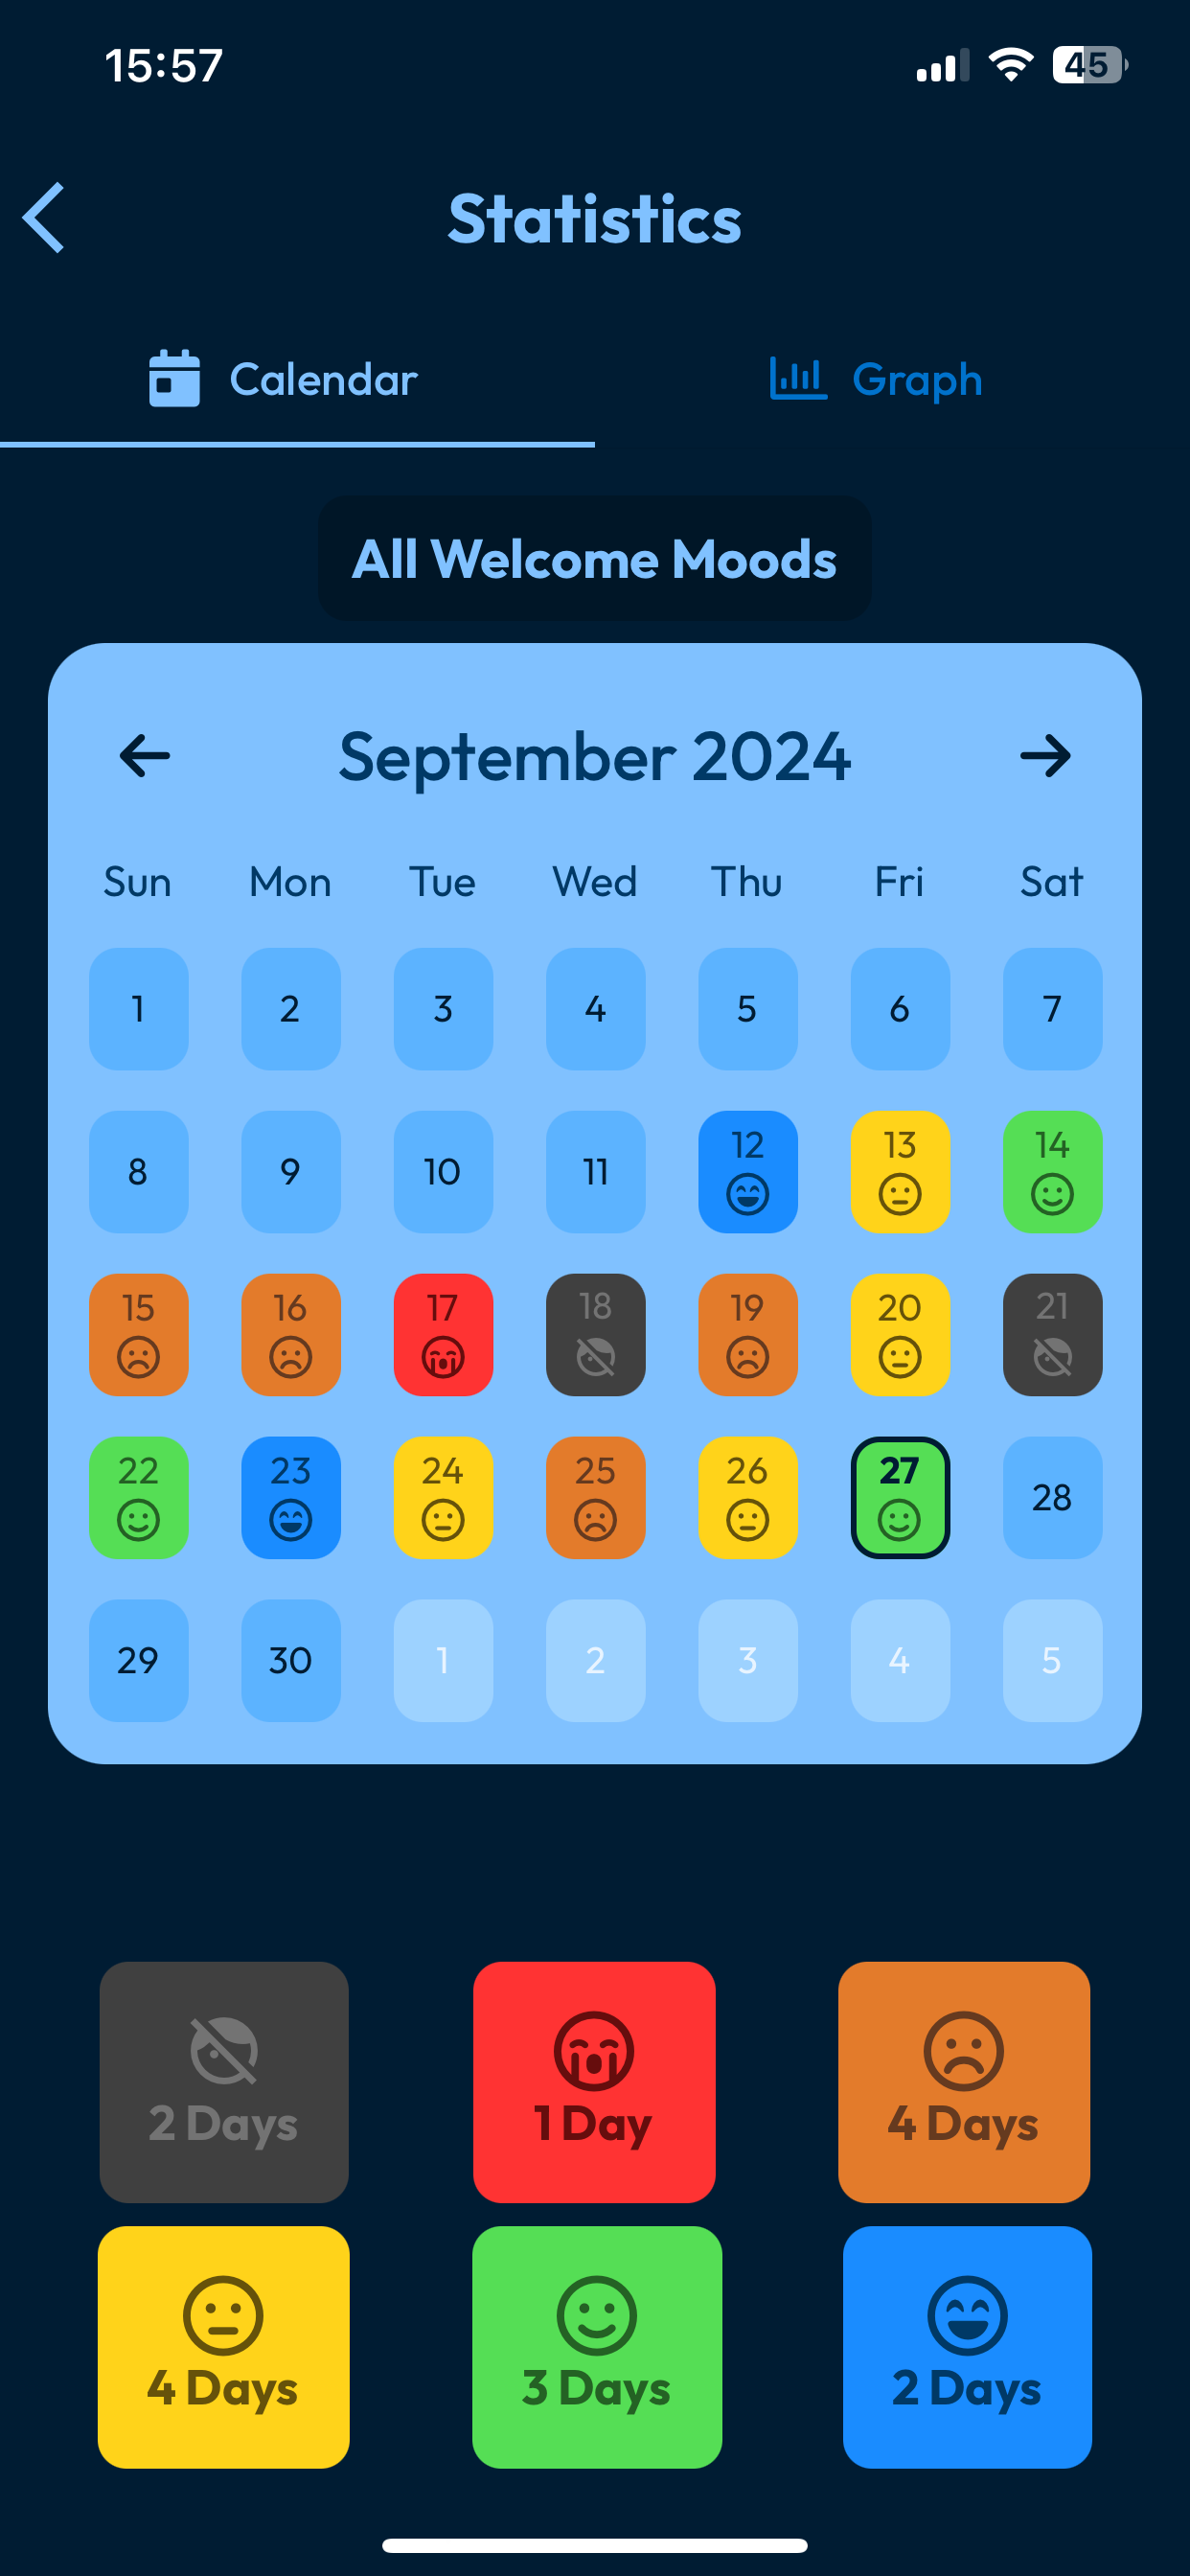
\includegraphics[scale=0.12]{figures/screenshots/Home - Calendar - Graph/2.PNG}\label{fig:calendar-page}}
    \hspace{10mm}
    \subfloat[Option On]{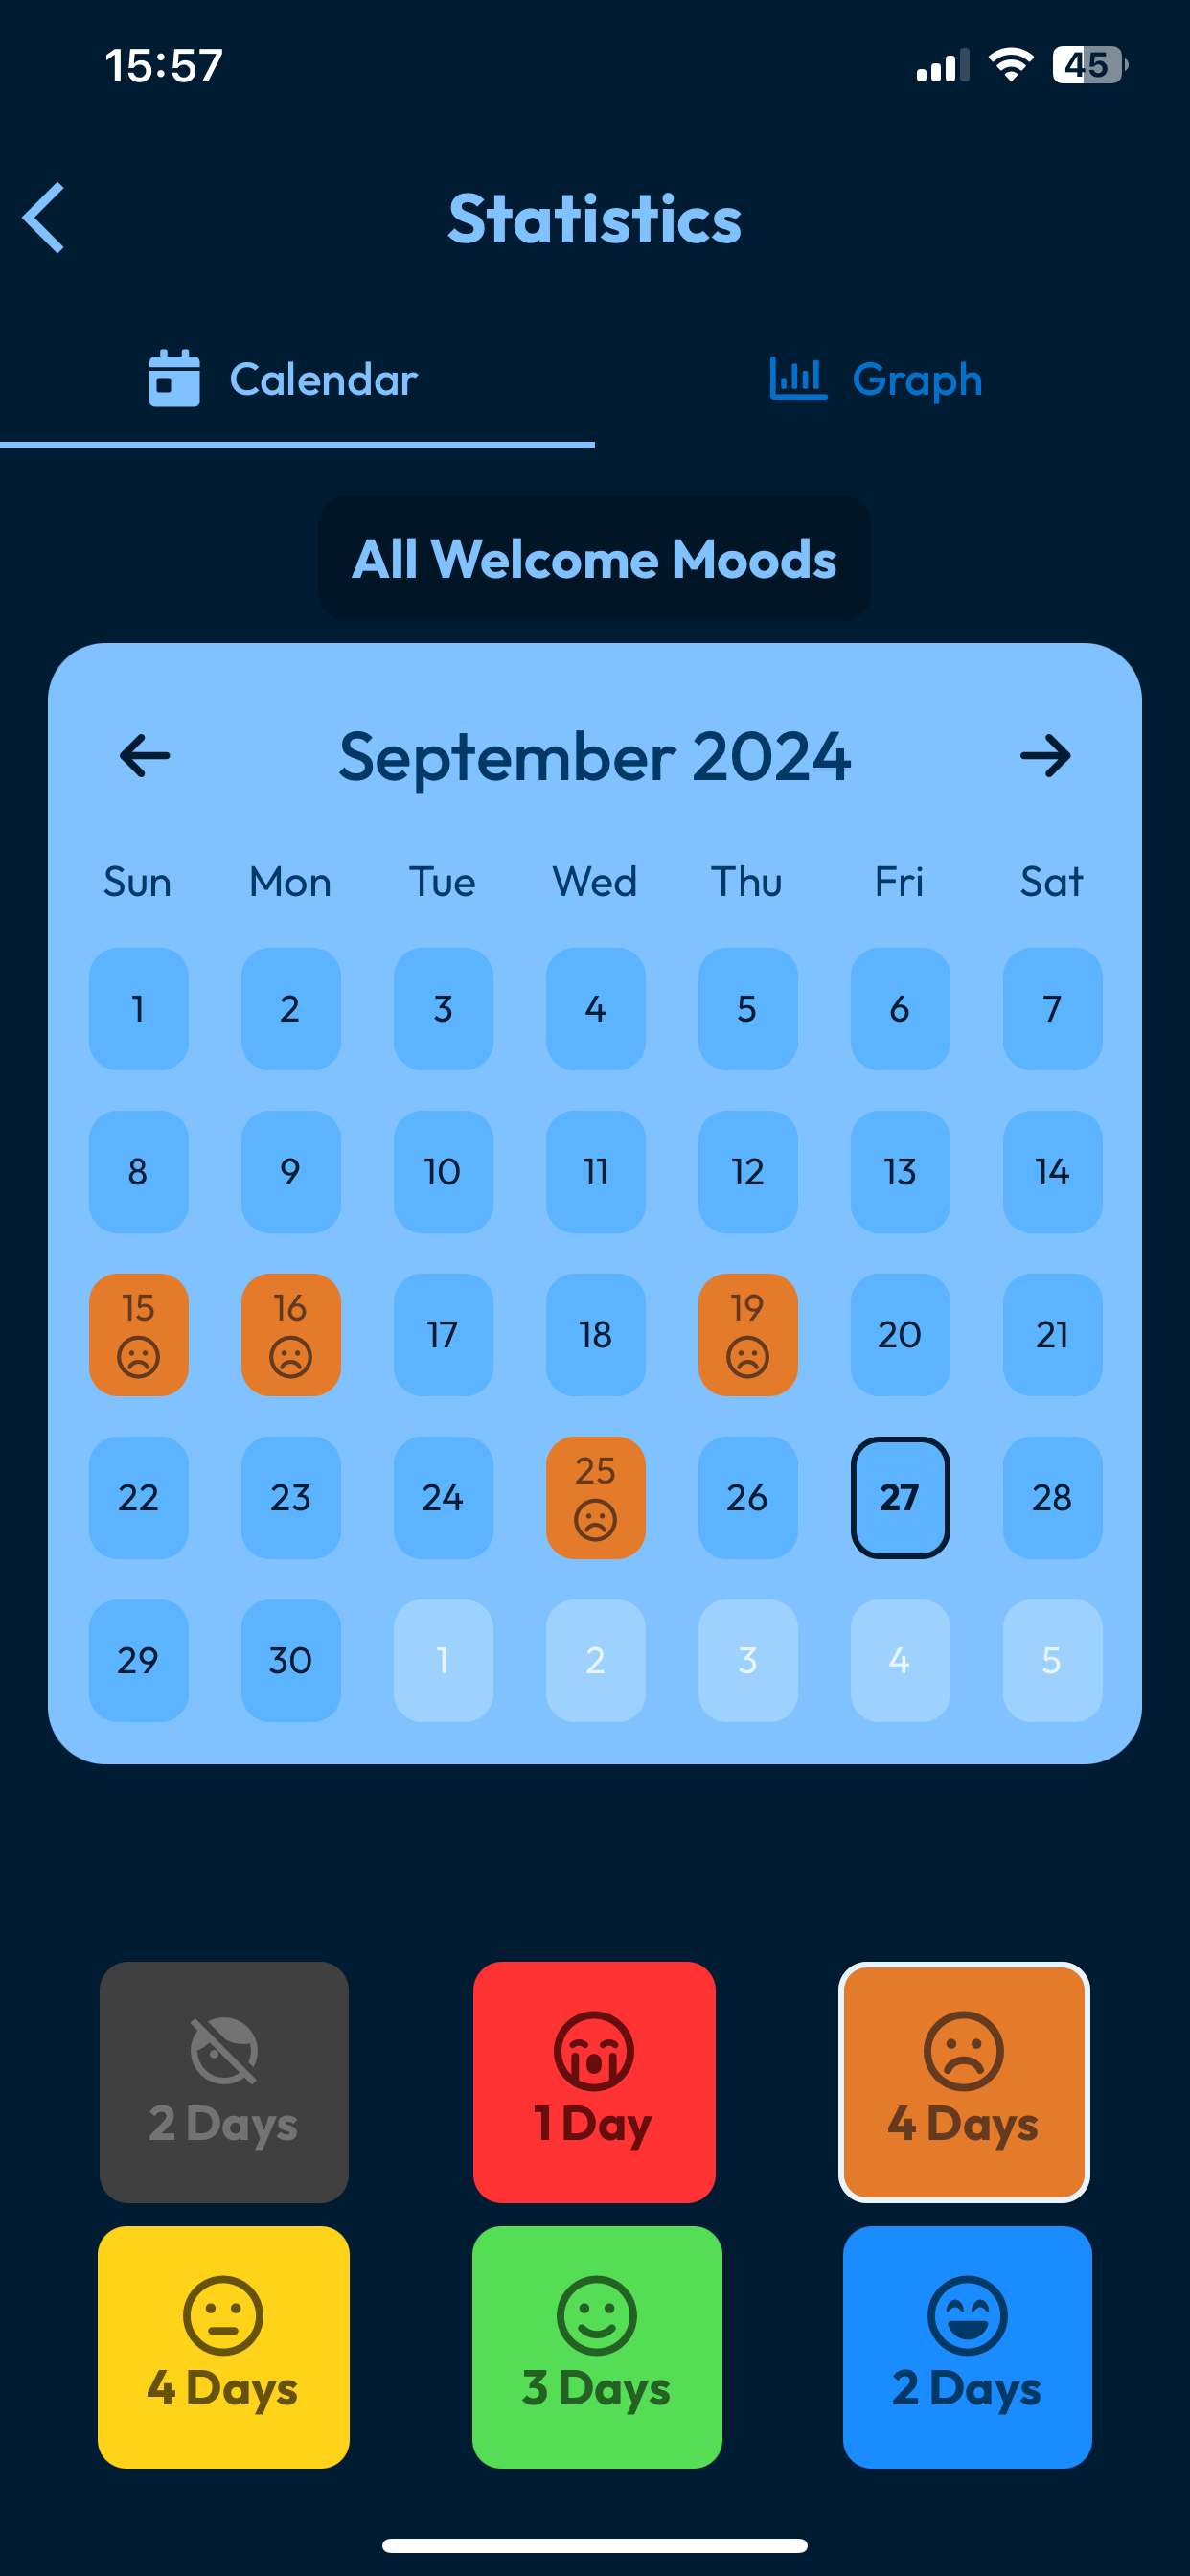
\includegraphics[scale=0.12]{figures/screenshots/Home - Calendar - Graph/3.PNG}\label{fig:calendar-option-on}}
    \caption{Calendar Screen - Pick a mood option from the calendar}
\end{figure}
\FloatBarrier

\vspace{5mm}

\subsection{Graph Screen}

The Graph Screen provides a detailed analysis of the user's mood data over a specified period. The main view consists of two different chart options such as a bar chart, and a pie chart that represent the user's mood variations. When a specific mood state is selected, the chart highlights the proportion or frequency of that mood over the selected period. There is also a legend below the pie chart that shows the colors of each mood and emoji.

\vspace{5mm}

\FloatBarrier
\begin{figure}[ht]
    \centering
    \subfloat[Graph Screen]{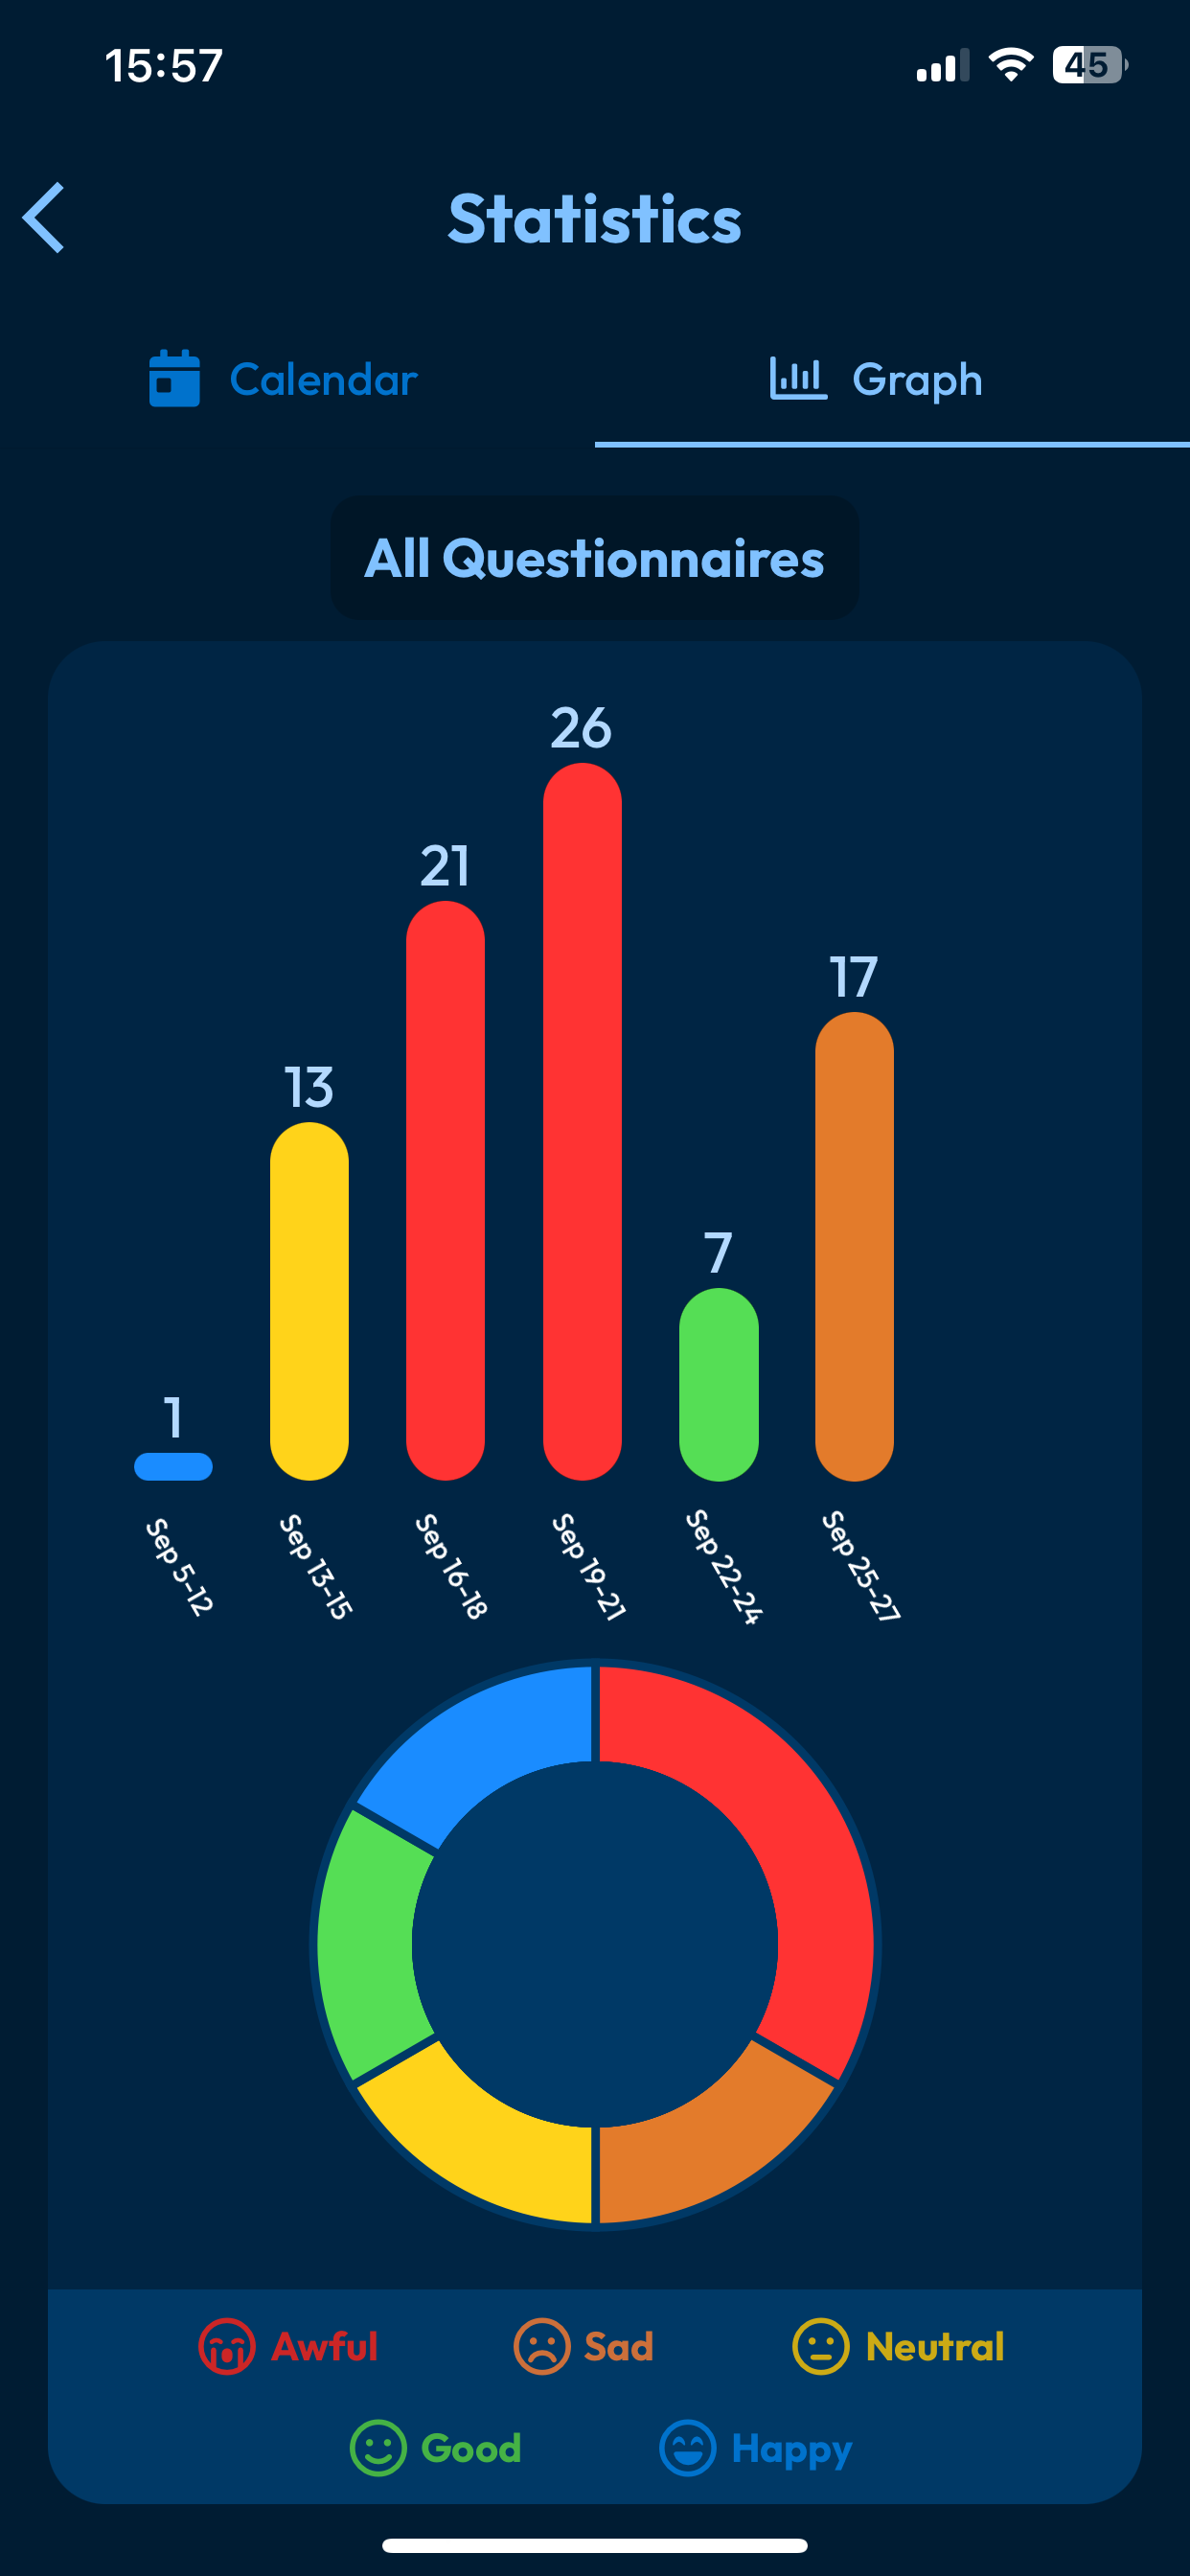
\includegraphics[scale=0.12]{figures/screenshots/Home - Calendar - Graph/4.PNG}\label{fig:graph-page}}
    \hspace{10mm}
    \subfloat[Pie chart option selected]{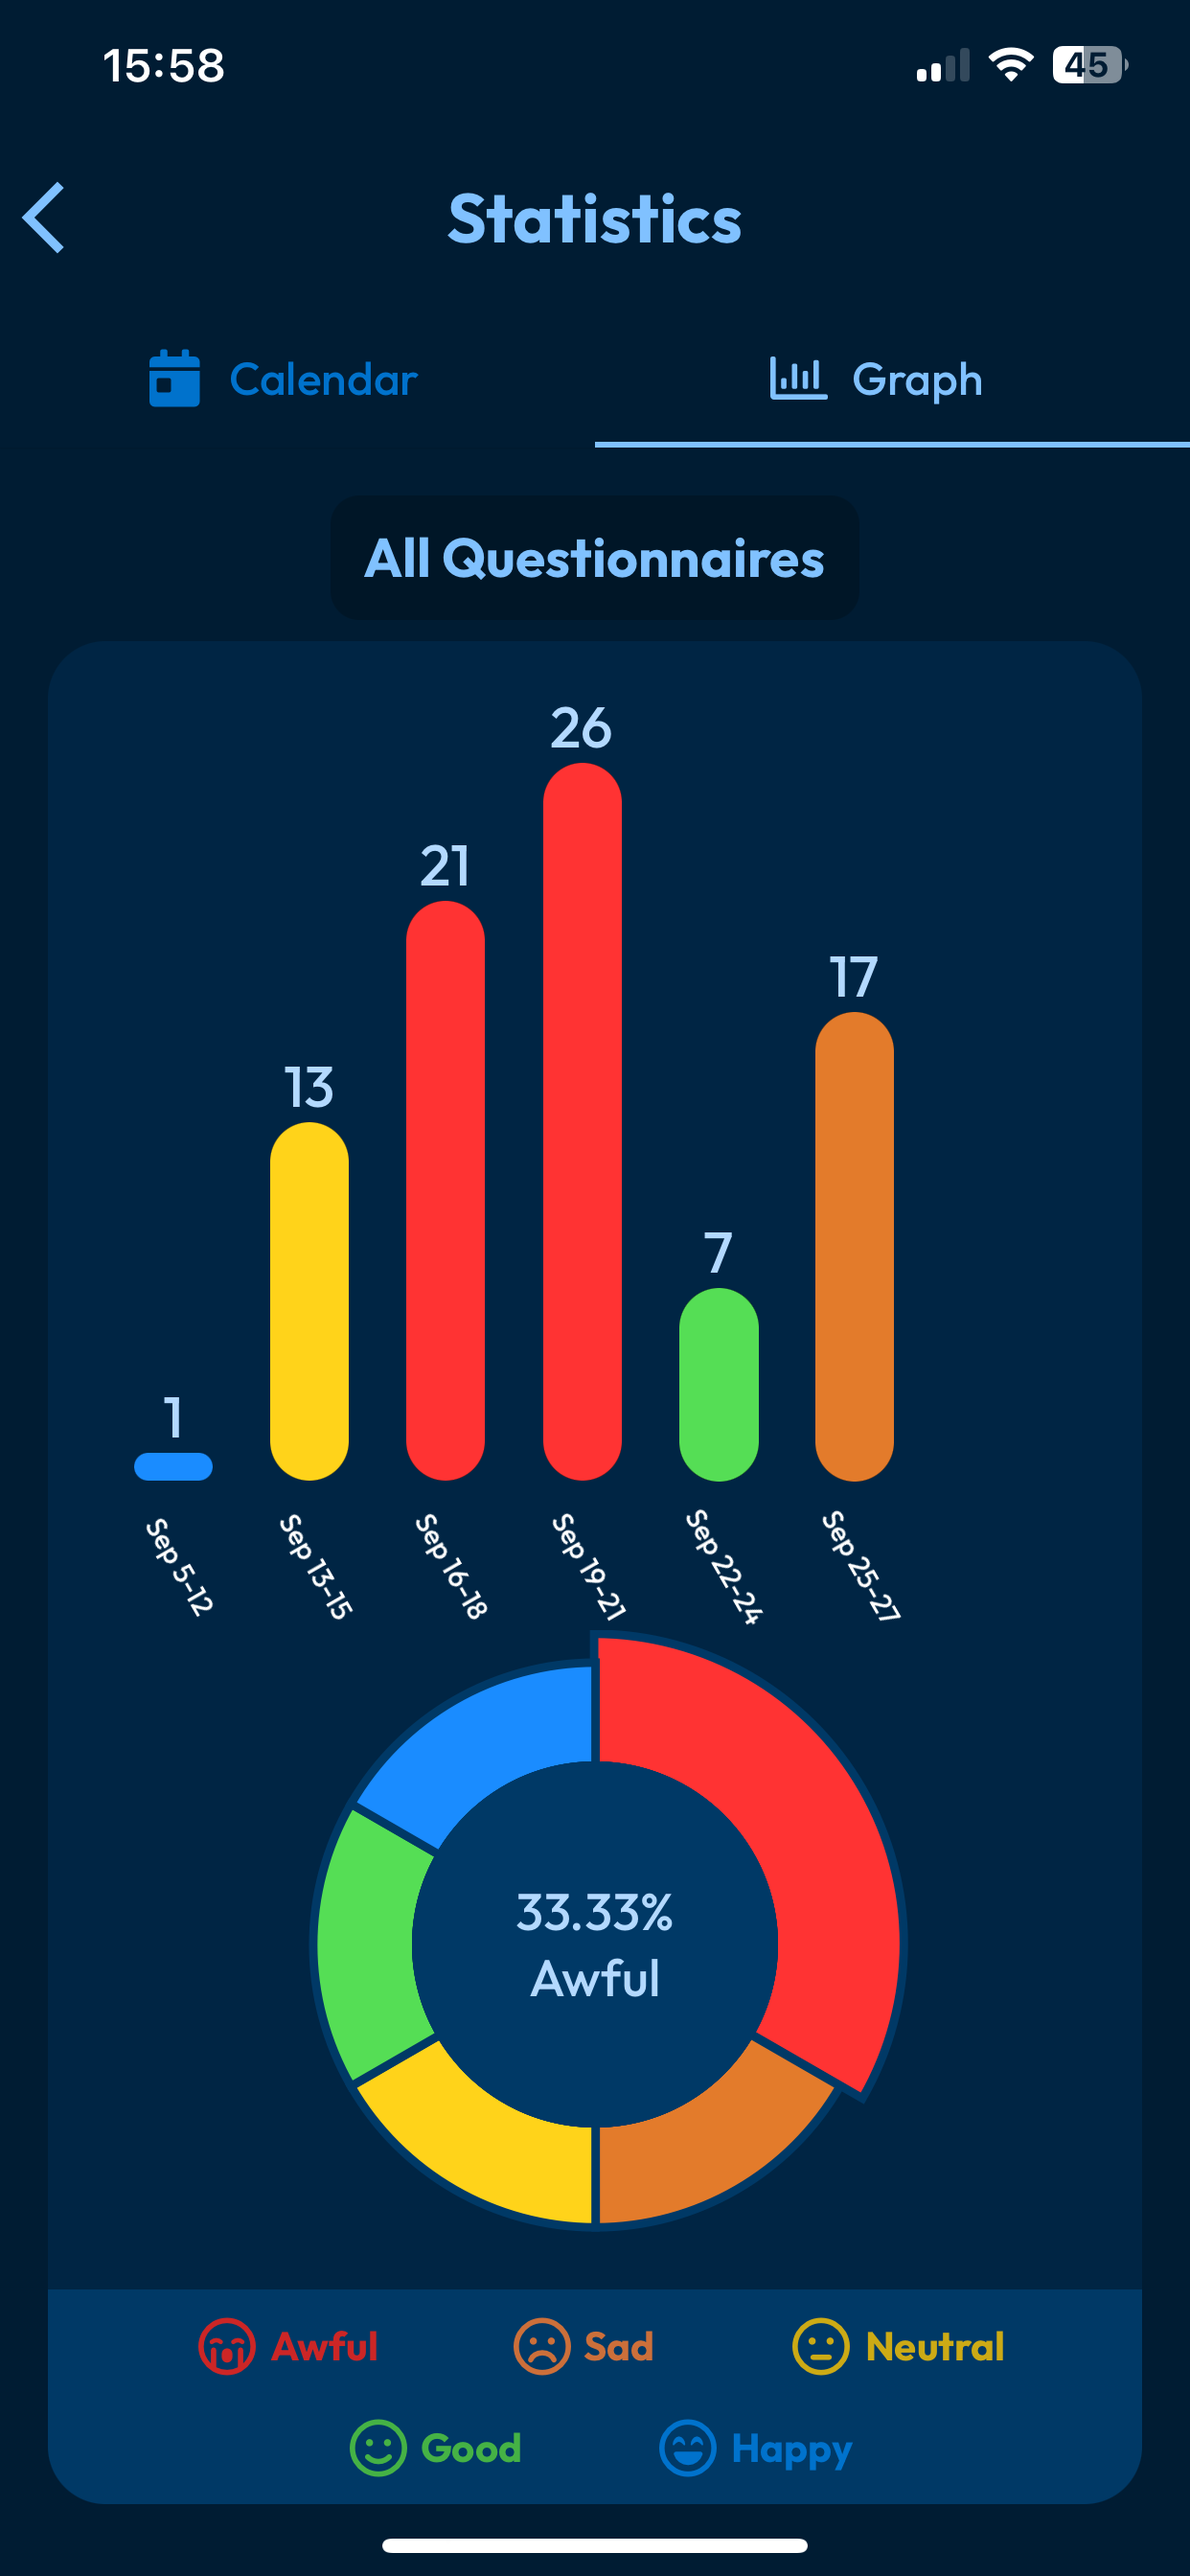
\includegraphics[scale=0.12]{figures/screenshots/Home - Calendar - Graph/5.PNG}\label{fig:pie-chart-option}}
    \caption{Graph Screen - Analysis of mood options using pie chart}
\end{figure}
\FloatBarrier

\vspace{5mm}

\subsection{Profile Screen}

\noindent \textbf{User's Avatar Image Modification} \\
The Profile screen allows users to view and update their avatar image. When a user wishes to modify their avatar image, the following steps can be taken:

\begin{itemize}
    \item \textbf{Initial State:} Click on the avatar image, and after that two optiions are going to be revealed on the right and left side of the avatar image.
    \item \textbf{Step 1:} Click the delete icon next to the user's avatar image (Fig. \ref{fig:user-image-step-1}).
    \item \textbf{Step 2:} A confirmation text shows on the top, indicating that you deleted the image succesfully (Fig. \ref{fig:user-image-step-2}).
    \item \textbf{Step 3:} Go back to the ``Home'' screen by presing the arror buton on the top left corner of the screen (Fig. \ref{fig:user-image-step-3}).
    \item \textbf{Step 4:} You can see that when there is not avatar image, the initials are shown instead of an image (on the top right corner of the screen) (Fig. \ref{fig:user-image-step-4}).
    \item \textbf{Step 5:} The user can update the avatar image by clicking the ``camera'' button, after which a confirmation message appears indicating successful updating (Fig. \ref{fig:user-image-step-5}).
\end{itemize}

\vspace{5mm}

\FloatBarrier
\begin{figure}[ht]
    \centering
    \subfloat[Step 1]{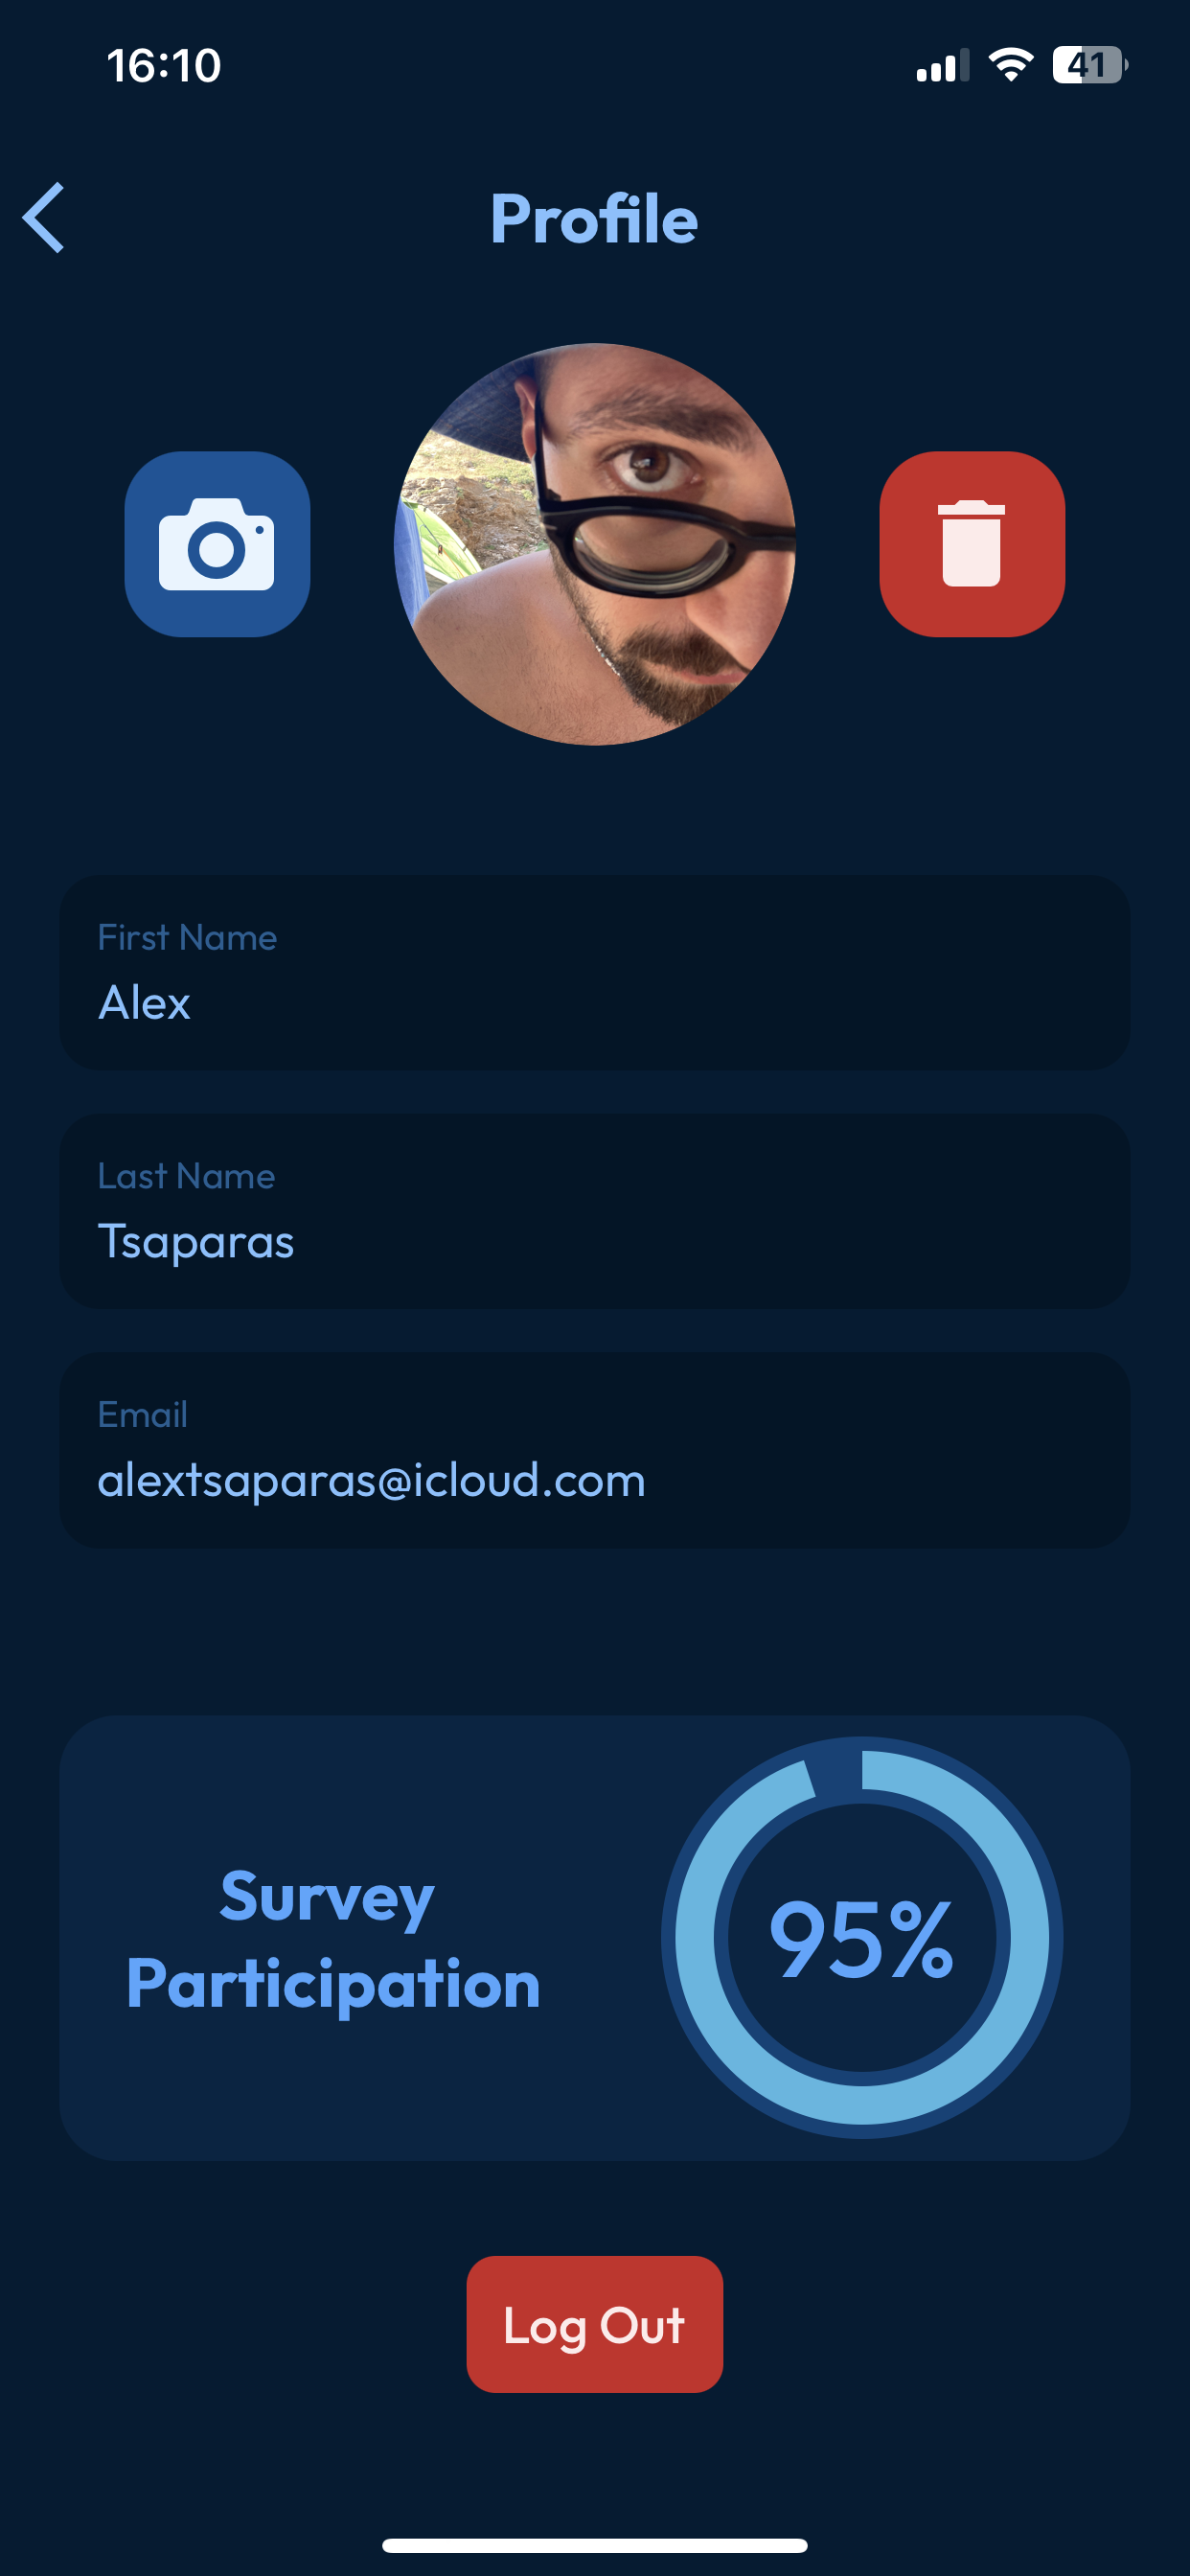
\includegraphics[scale=0.11]{figures/screenshots/Update User Image/1.PNG}\label{fig:user-image-step-1}}
    \hfill
    \subfloat[Step 2]{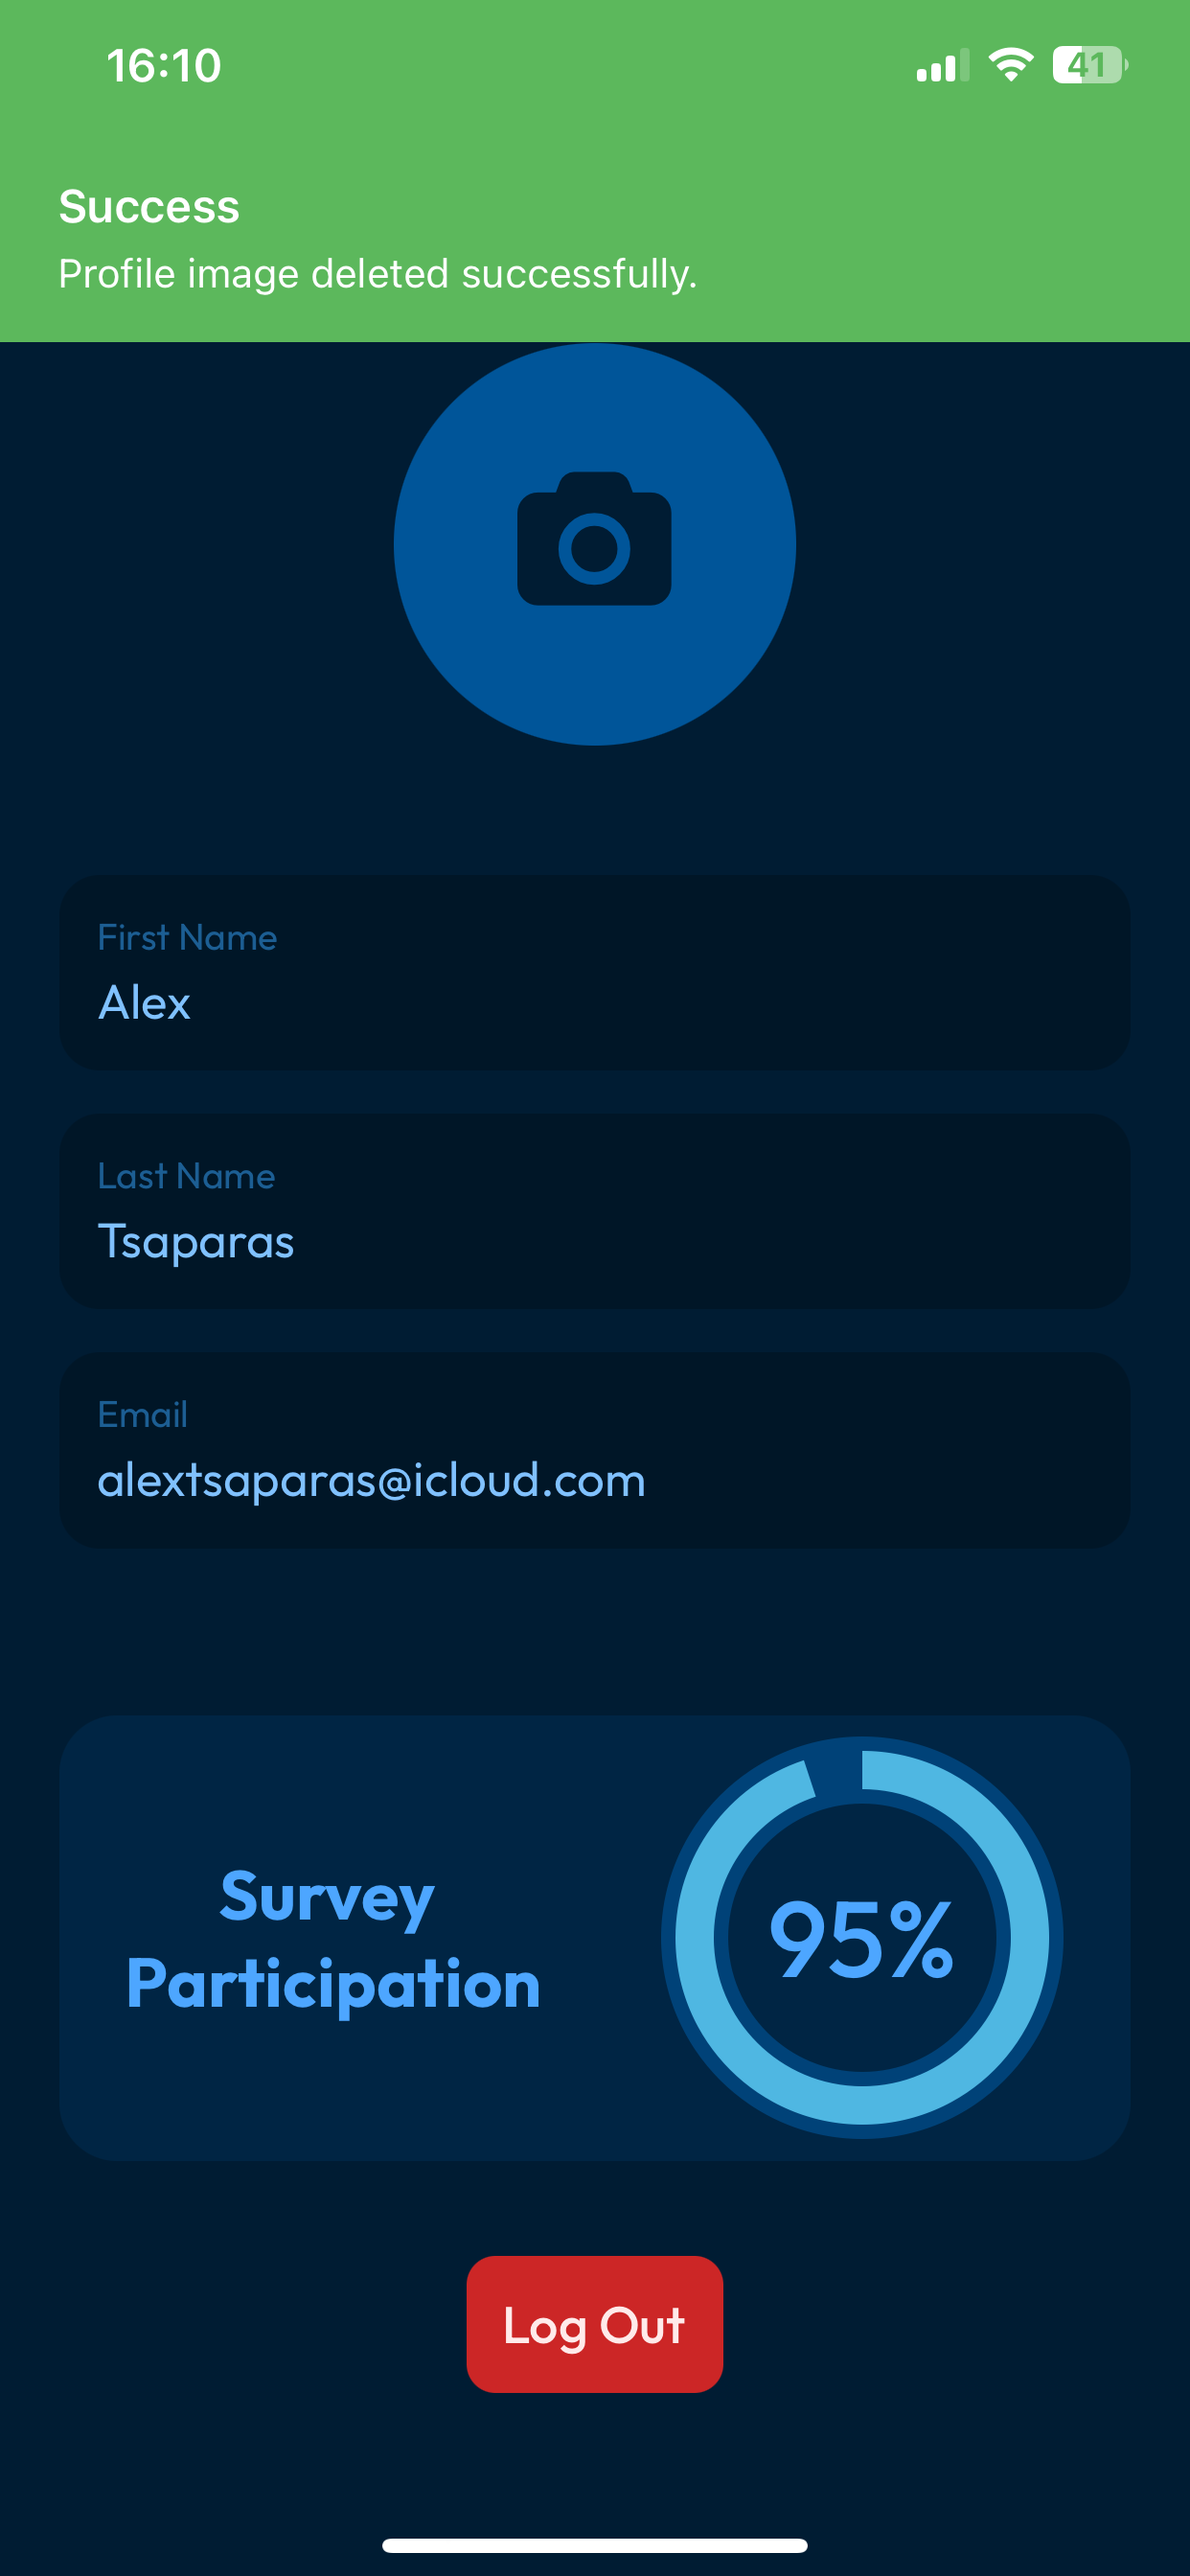
\includegraphics[scale=0.11]{figures/screenshots/Update User Image/2.PNG}\label{fig:user-image-step-2}}
    \hfill
    \subfloat[Step 3]{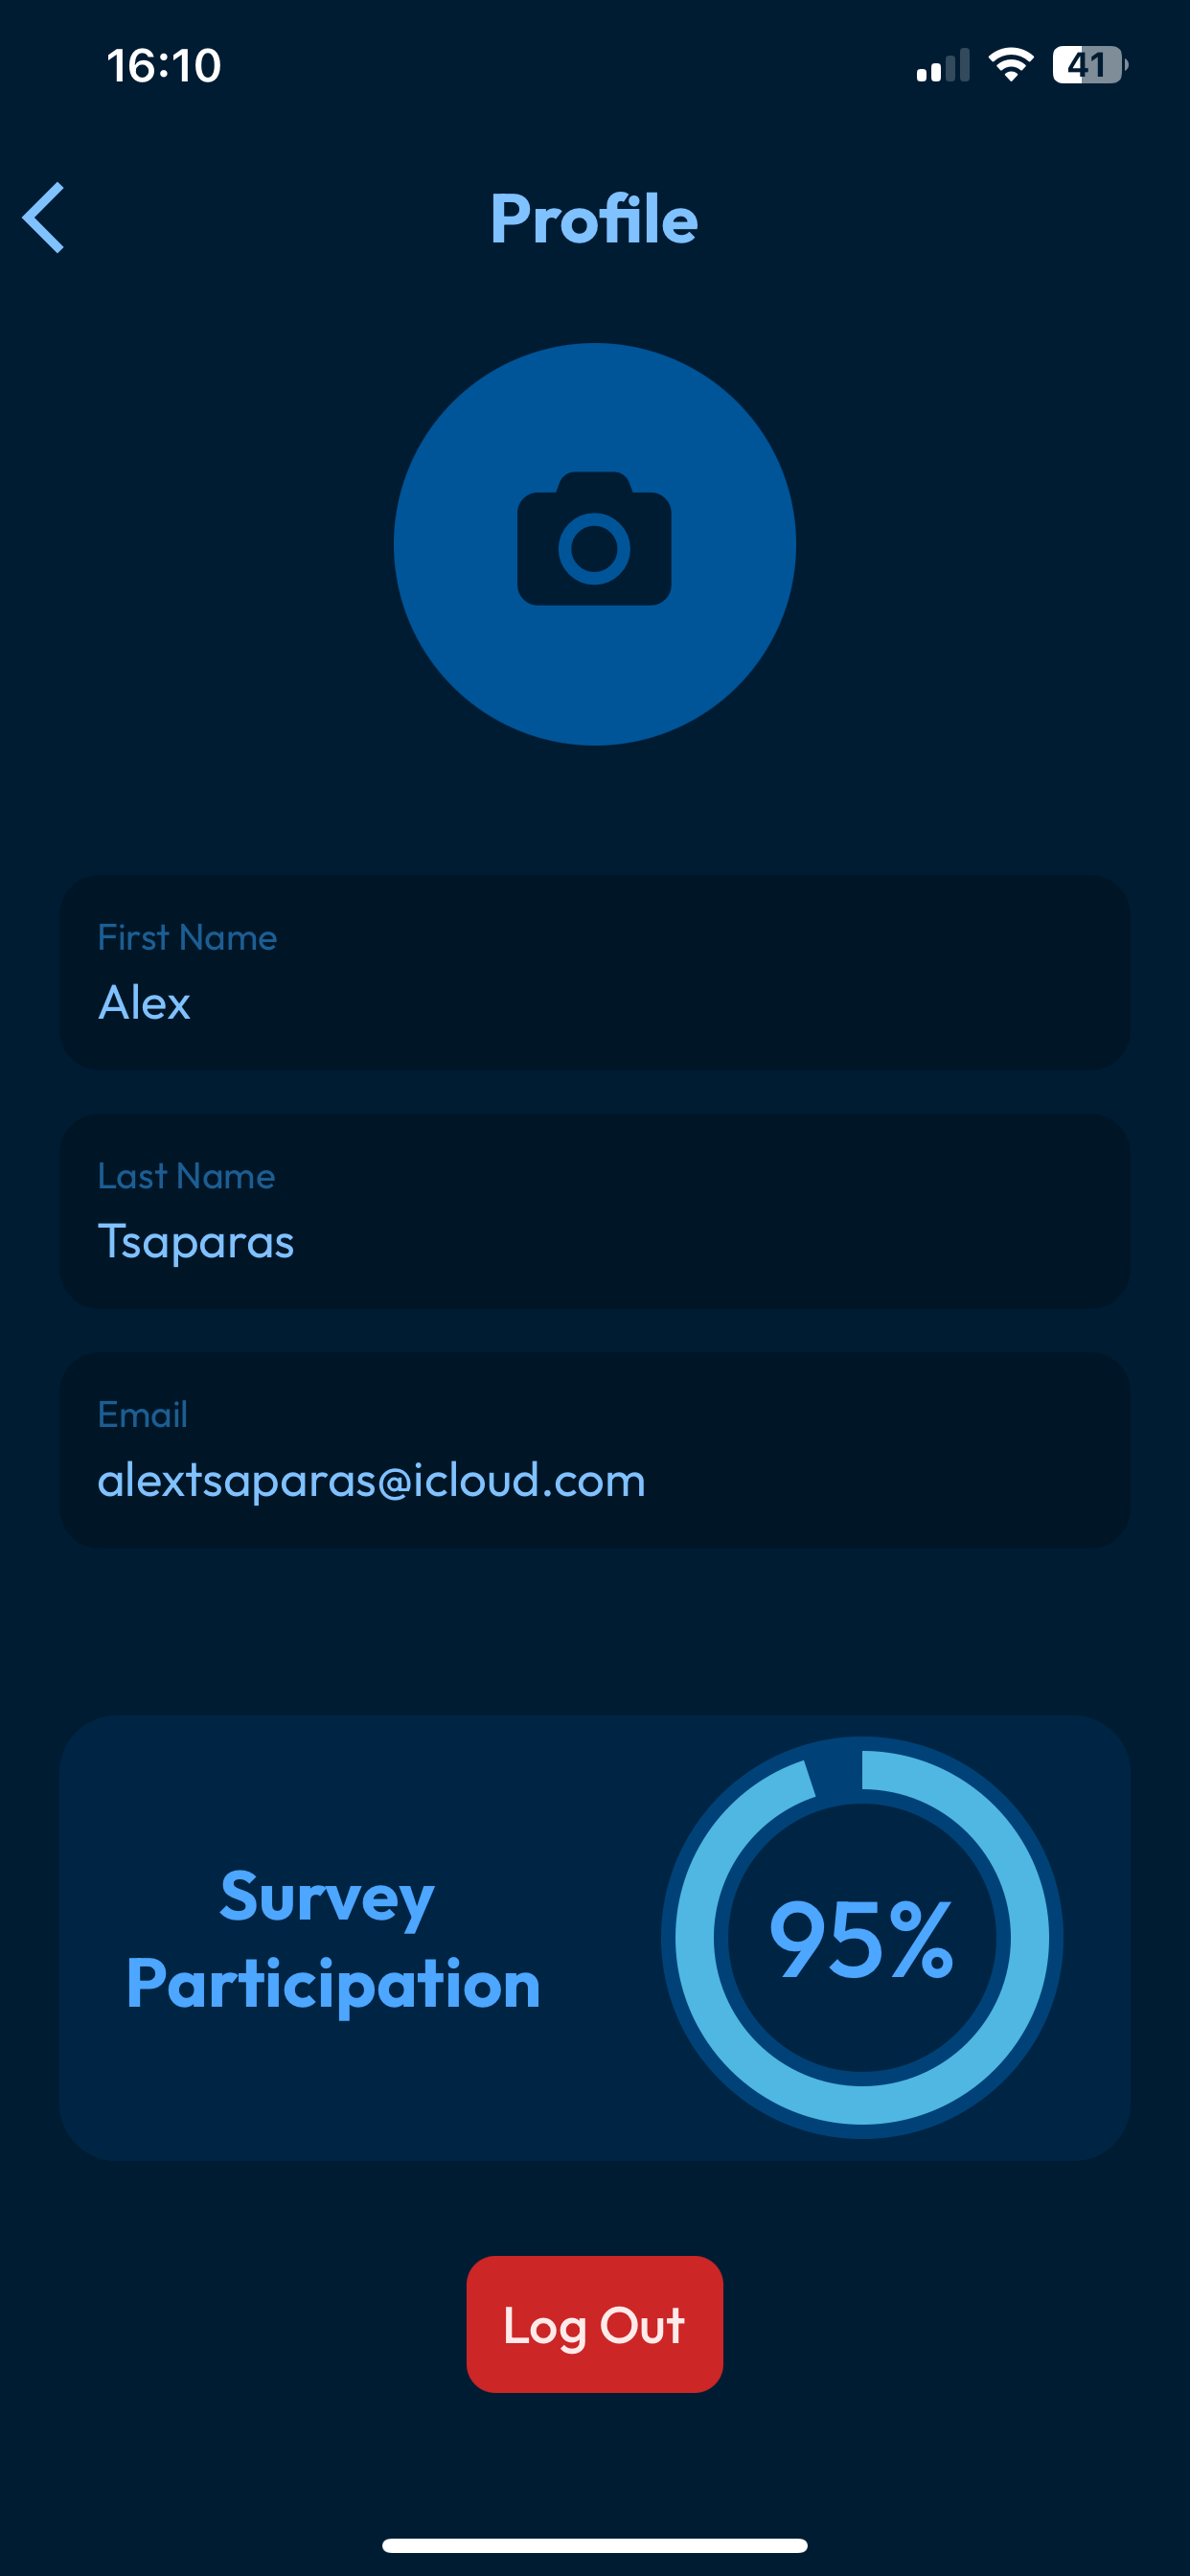
\includegraphics[scale=0.11]{figures/screenshots/Update User Image/3.PNG}\label{fig:user-image-step-3}}
\end{figure}
\FloatBarrier

\FloatBarrier
\begin{figure}[ht]\ContinuedFloat
    \centering
    \subfloat[Step 4]{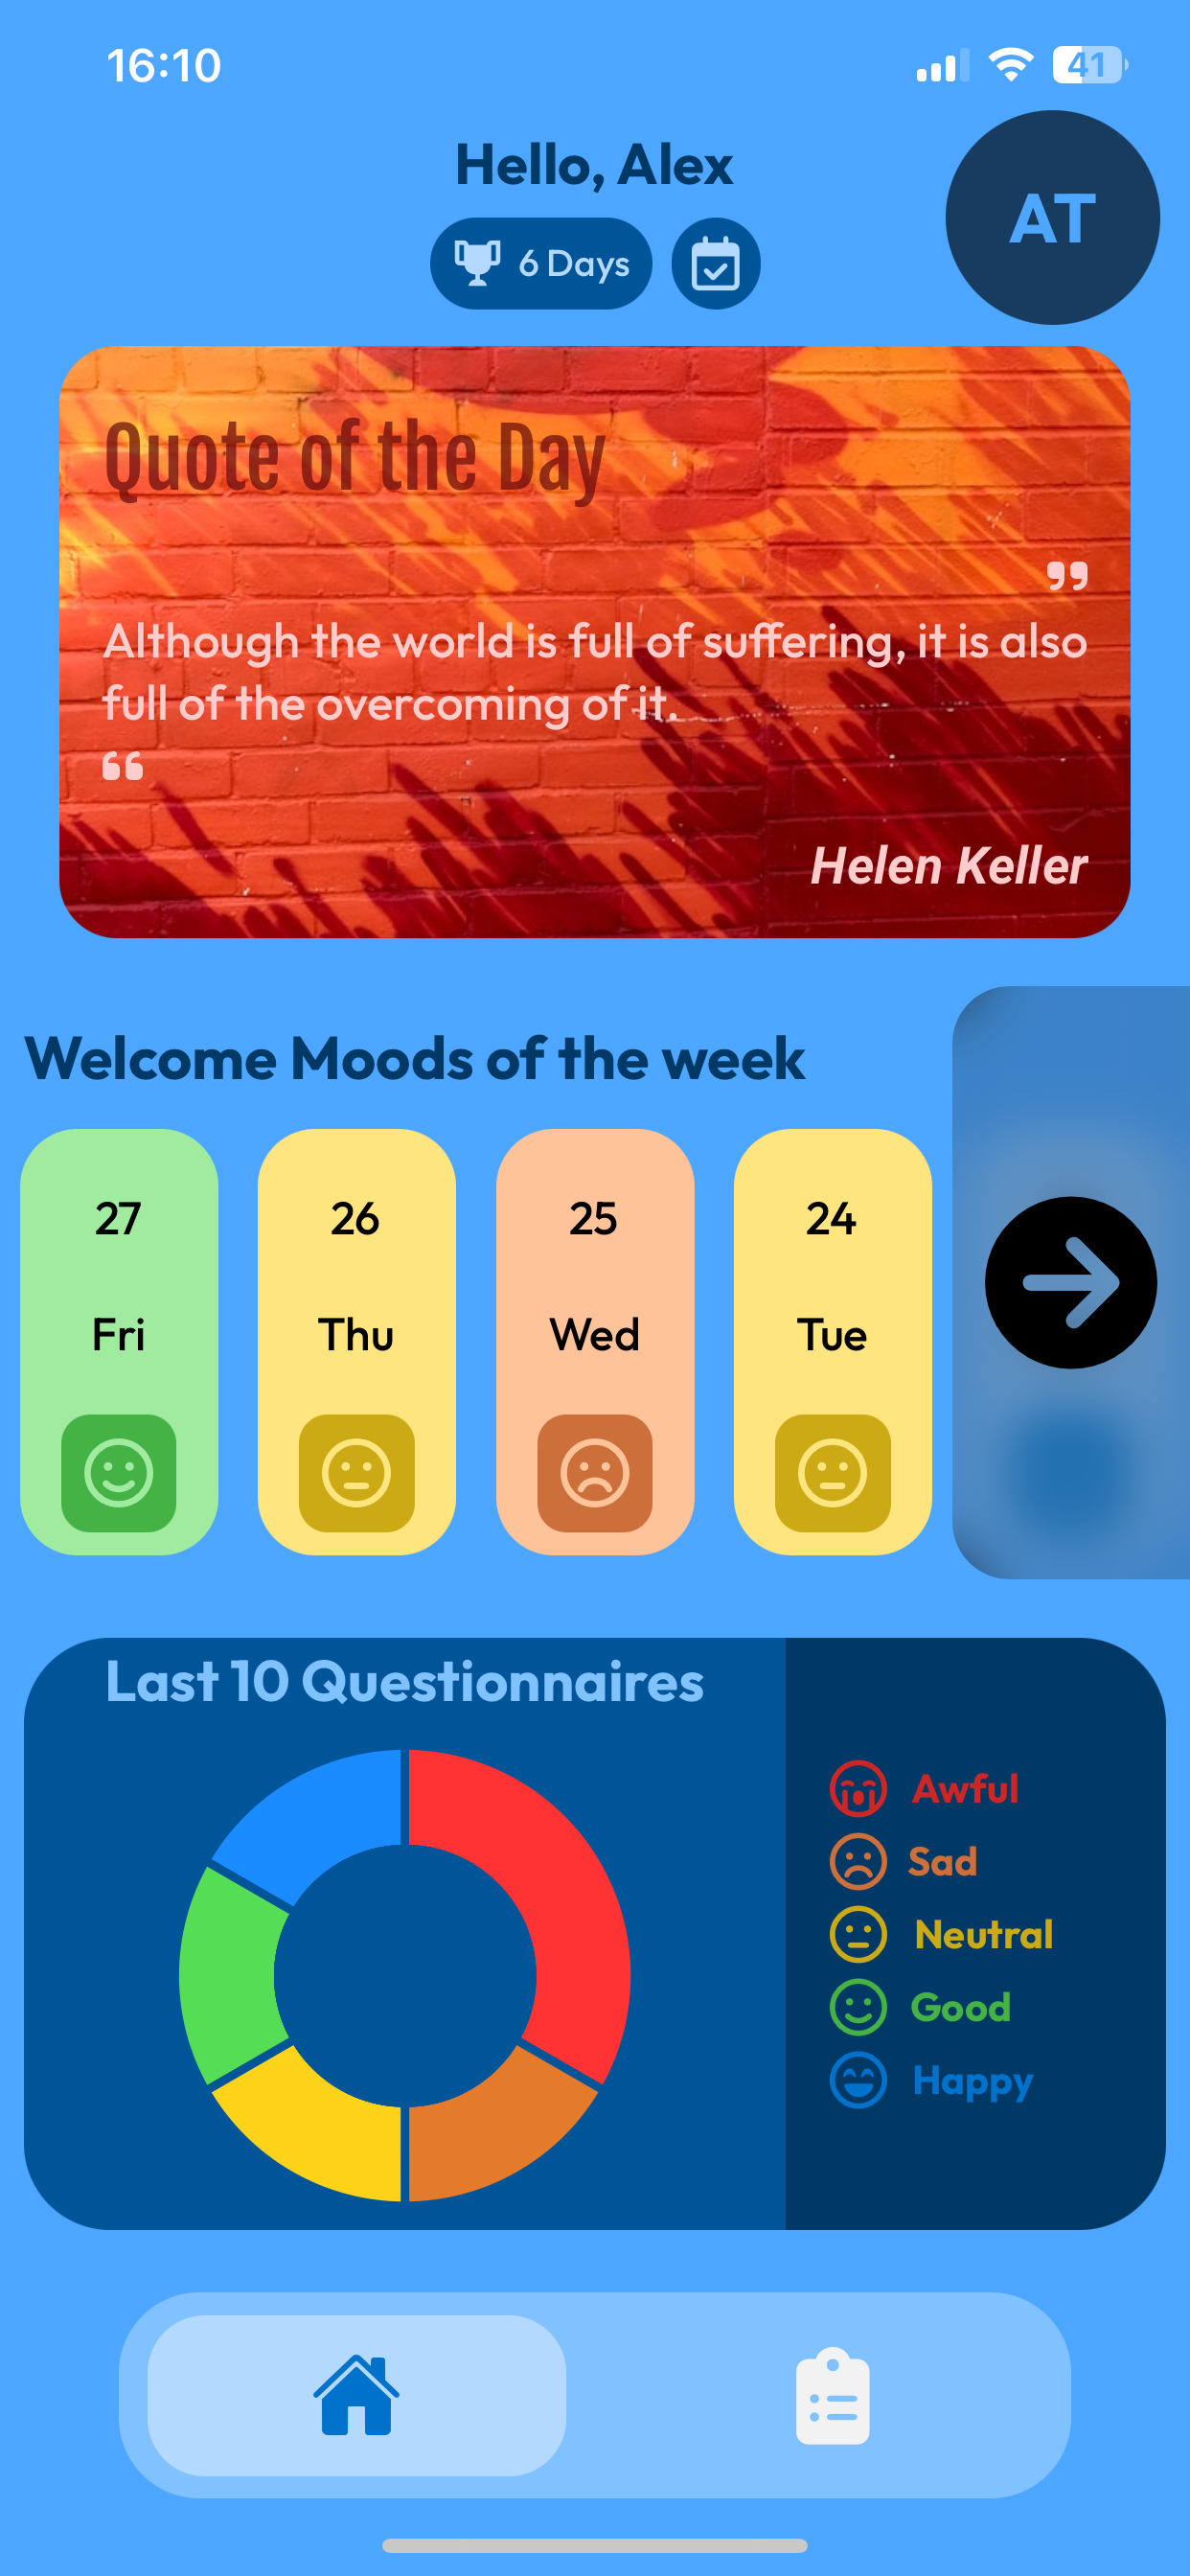
\includegraphics[scale=0.11]{figures/screenshots/Update User Image/4.PNG}\label{fig:user-image-step-4}}
    \hspace{10mm}
    \subfloat[Step 5]{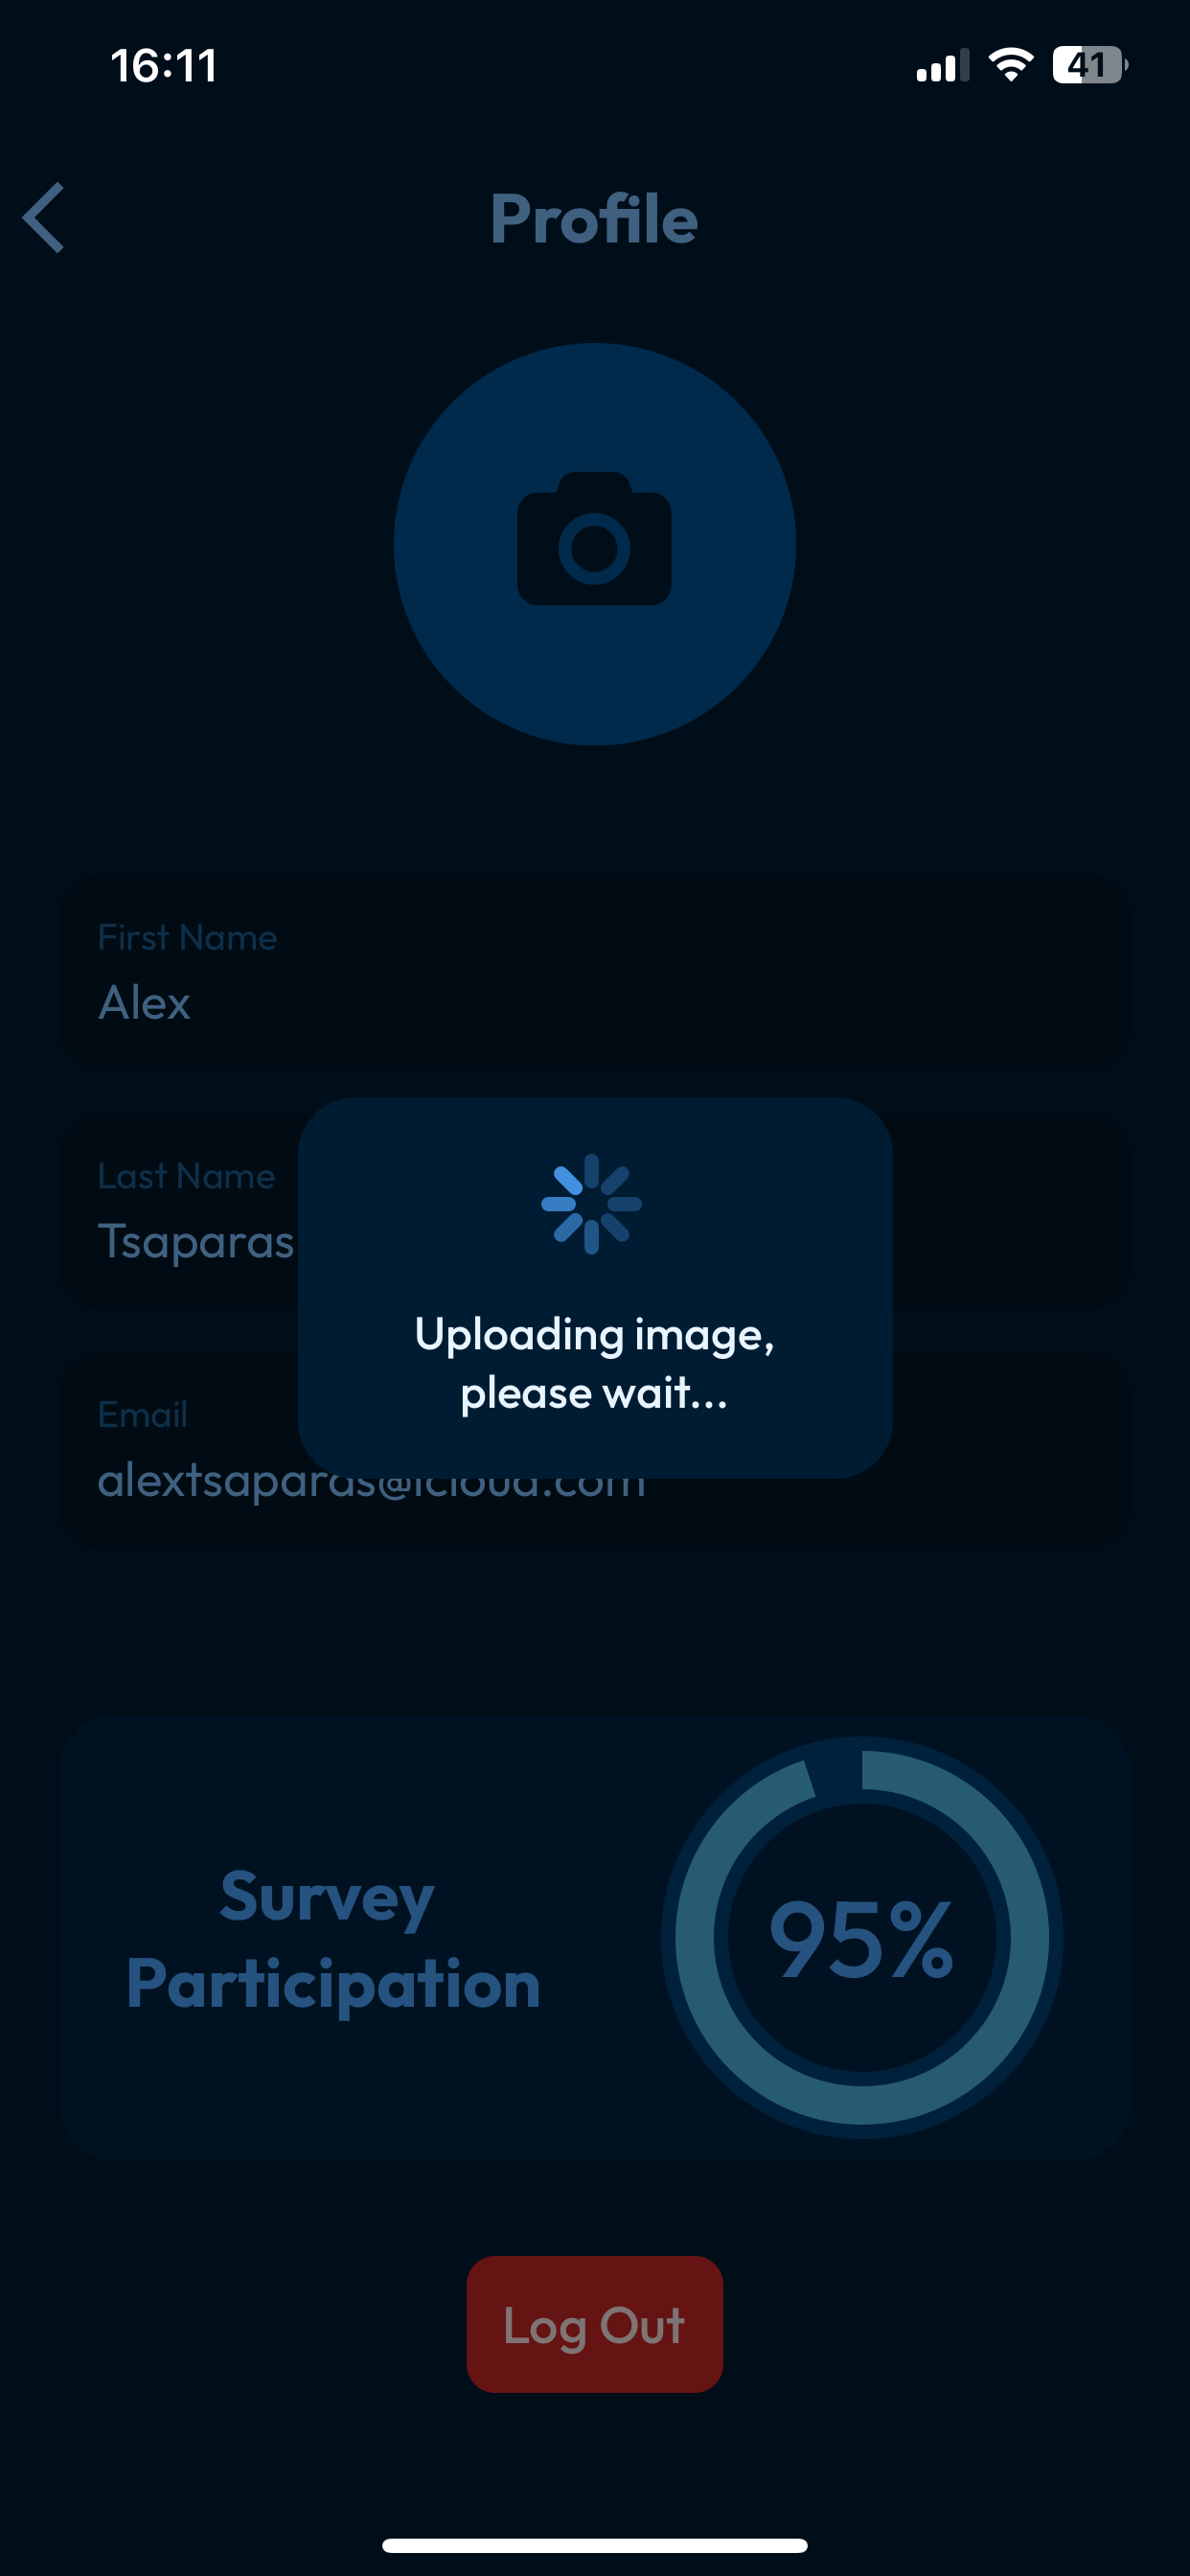
\includegraphics[scale=0.11]{figures/screenshots/Update User Image/5.PNG}\label{fig:user-image-step-5}}
    \caption{Procedure - Delete and Add the user's avatar image}
\end{figure}
\FloatBarrier

\vspace{10mm}

\noindent \textbf{User's Information Modification} \\
The Profile screen also allows users to modify their personal information such as their first name, last name or email. The steps involved in updating a user's information are outlined below:

\begin{itemize}
    \item \textbf{Step 1:} Click on the input field corresponding to the information to be changed (Fig. \ref{fig:user-info-step-1}).
    \item \textbf{Step 2:} Enter the new value in the input field (Fig. \ref{fig:user-info-step-2}).
    \item \textbf{Step 3:} Click on the ``Done'' button to confirm the changes (Fig. \ref{fig:user-info-step-3}).
    \item \textbf{Step 4:} A confirmation message appears at the top of the screen indicating that the changes have been successfully applied (Fig. \ref{fig:user-info-step-4}).
\end{itemize}

\vspace{5mm}

\FloatBarrier
\begin{figure}[ht]
    \centering
    \subfloat[Step 1]{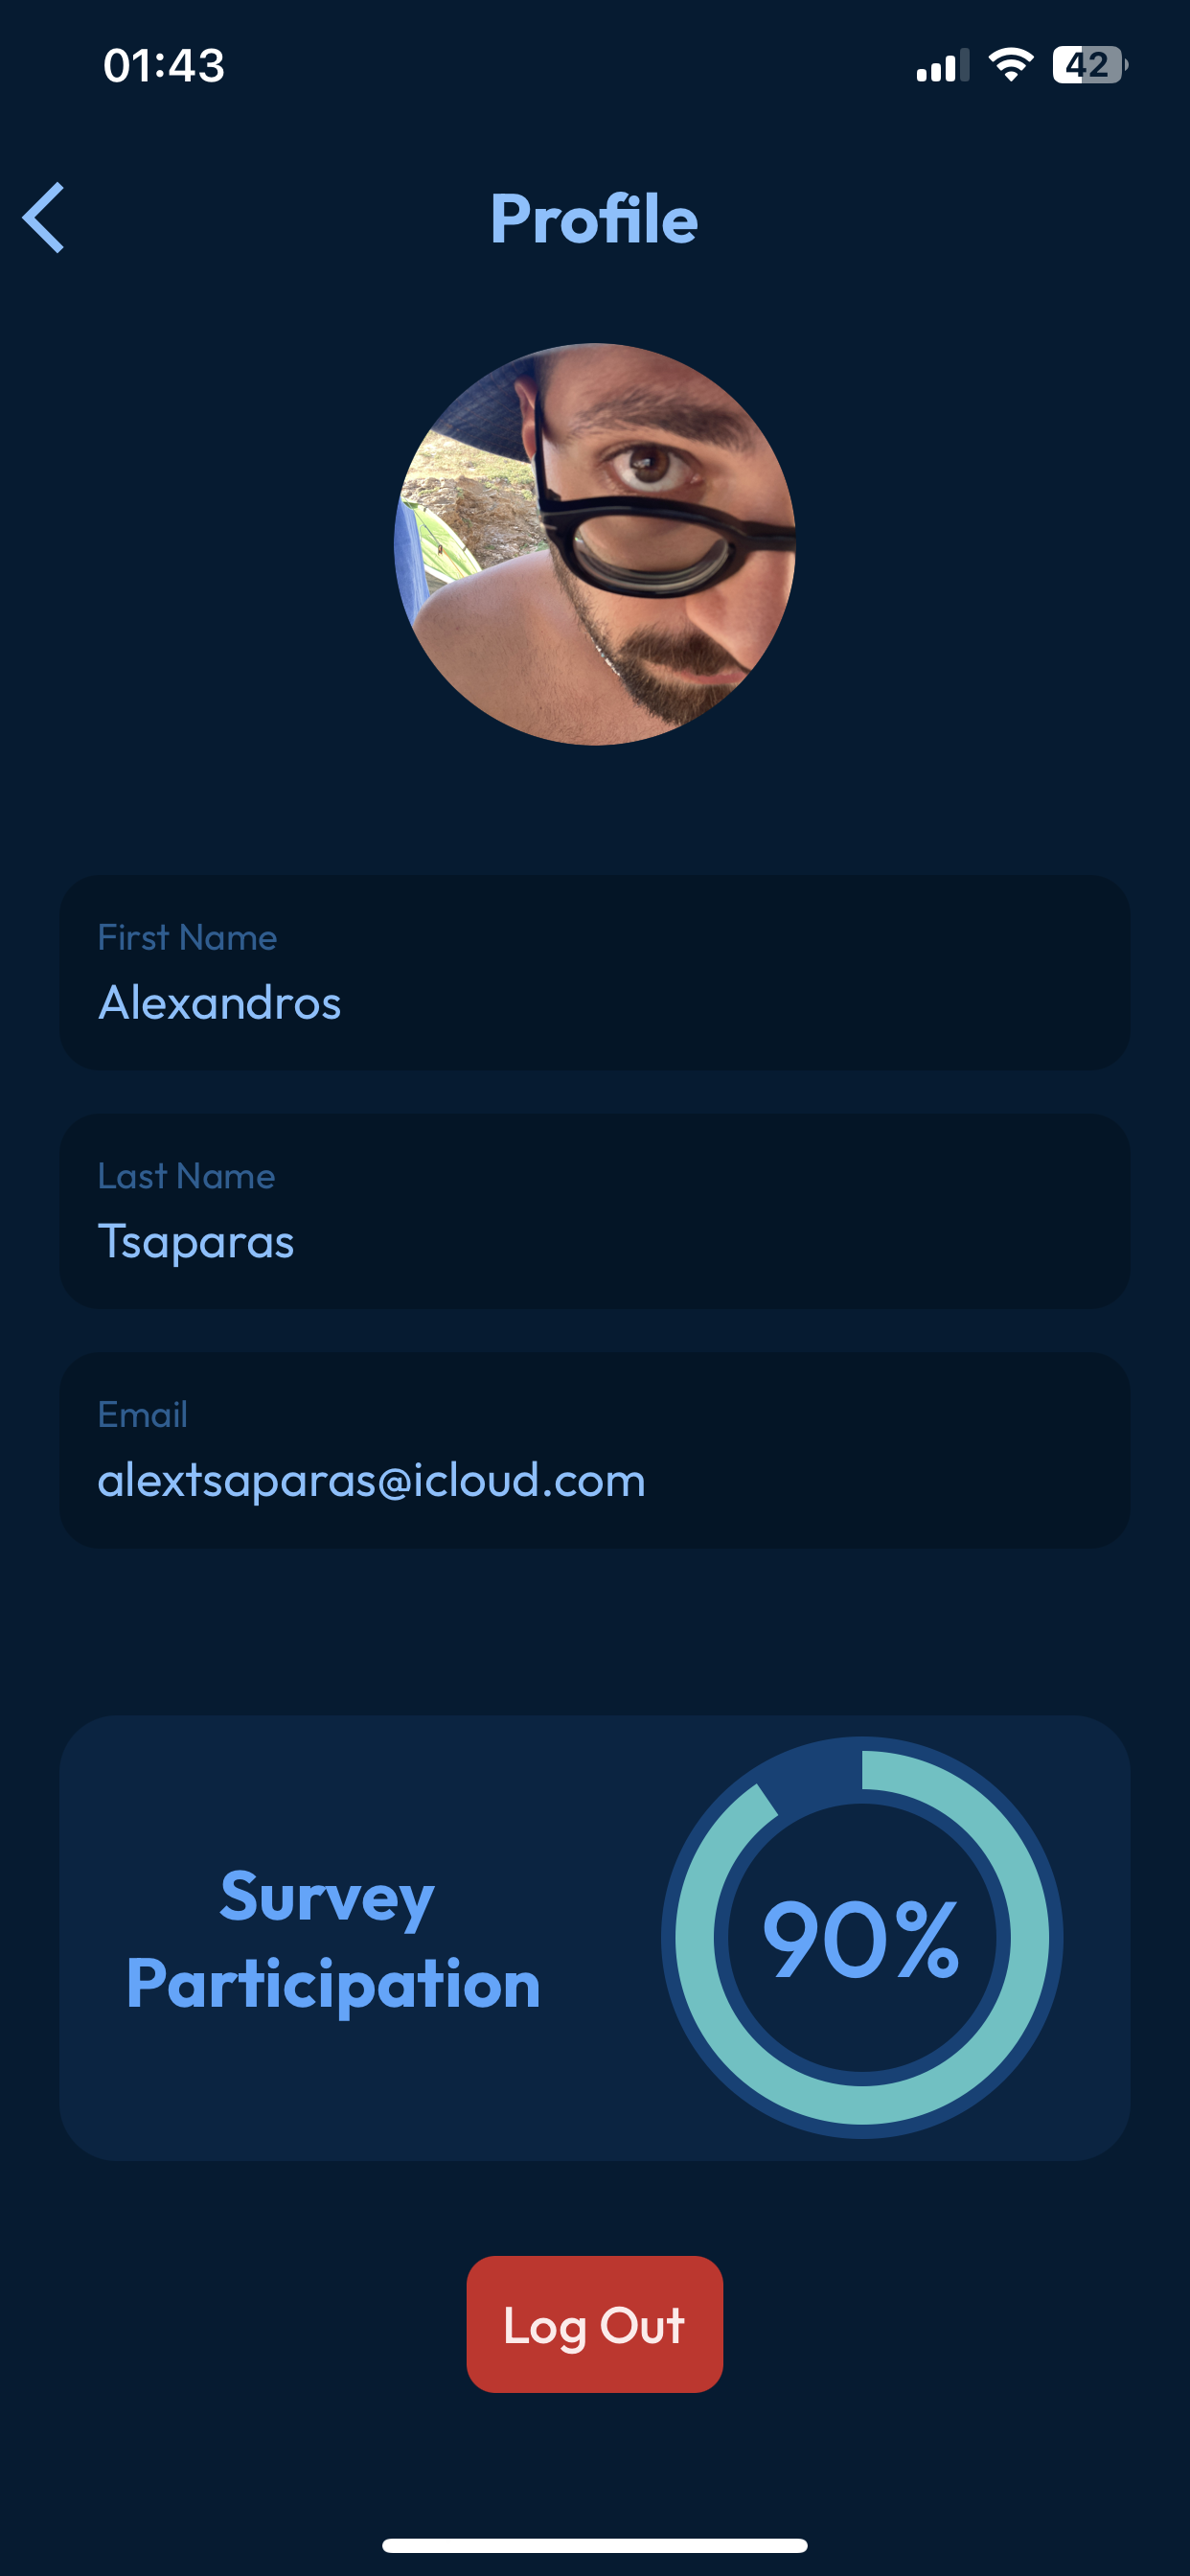
\includegraphics[scale=0.11]{figures/screenshots/Update User Info/1.PNG}\label{fig:user-info-step-1}}
    \hspace{2mm}
    \subfloat[Step 2]{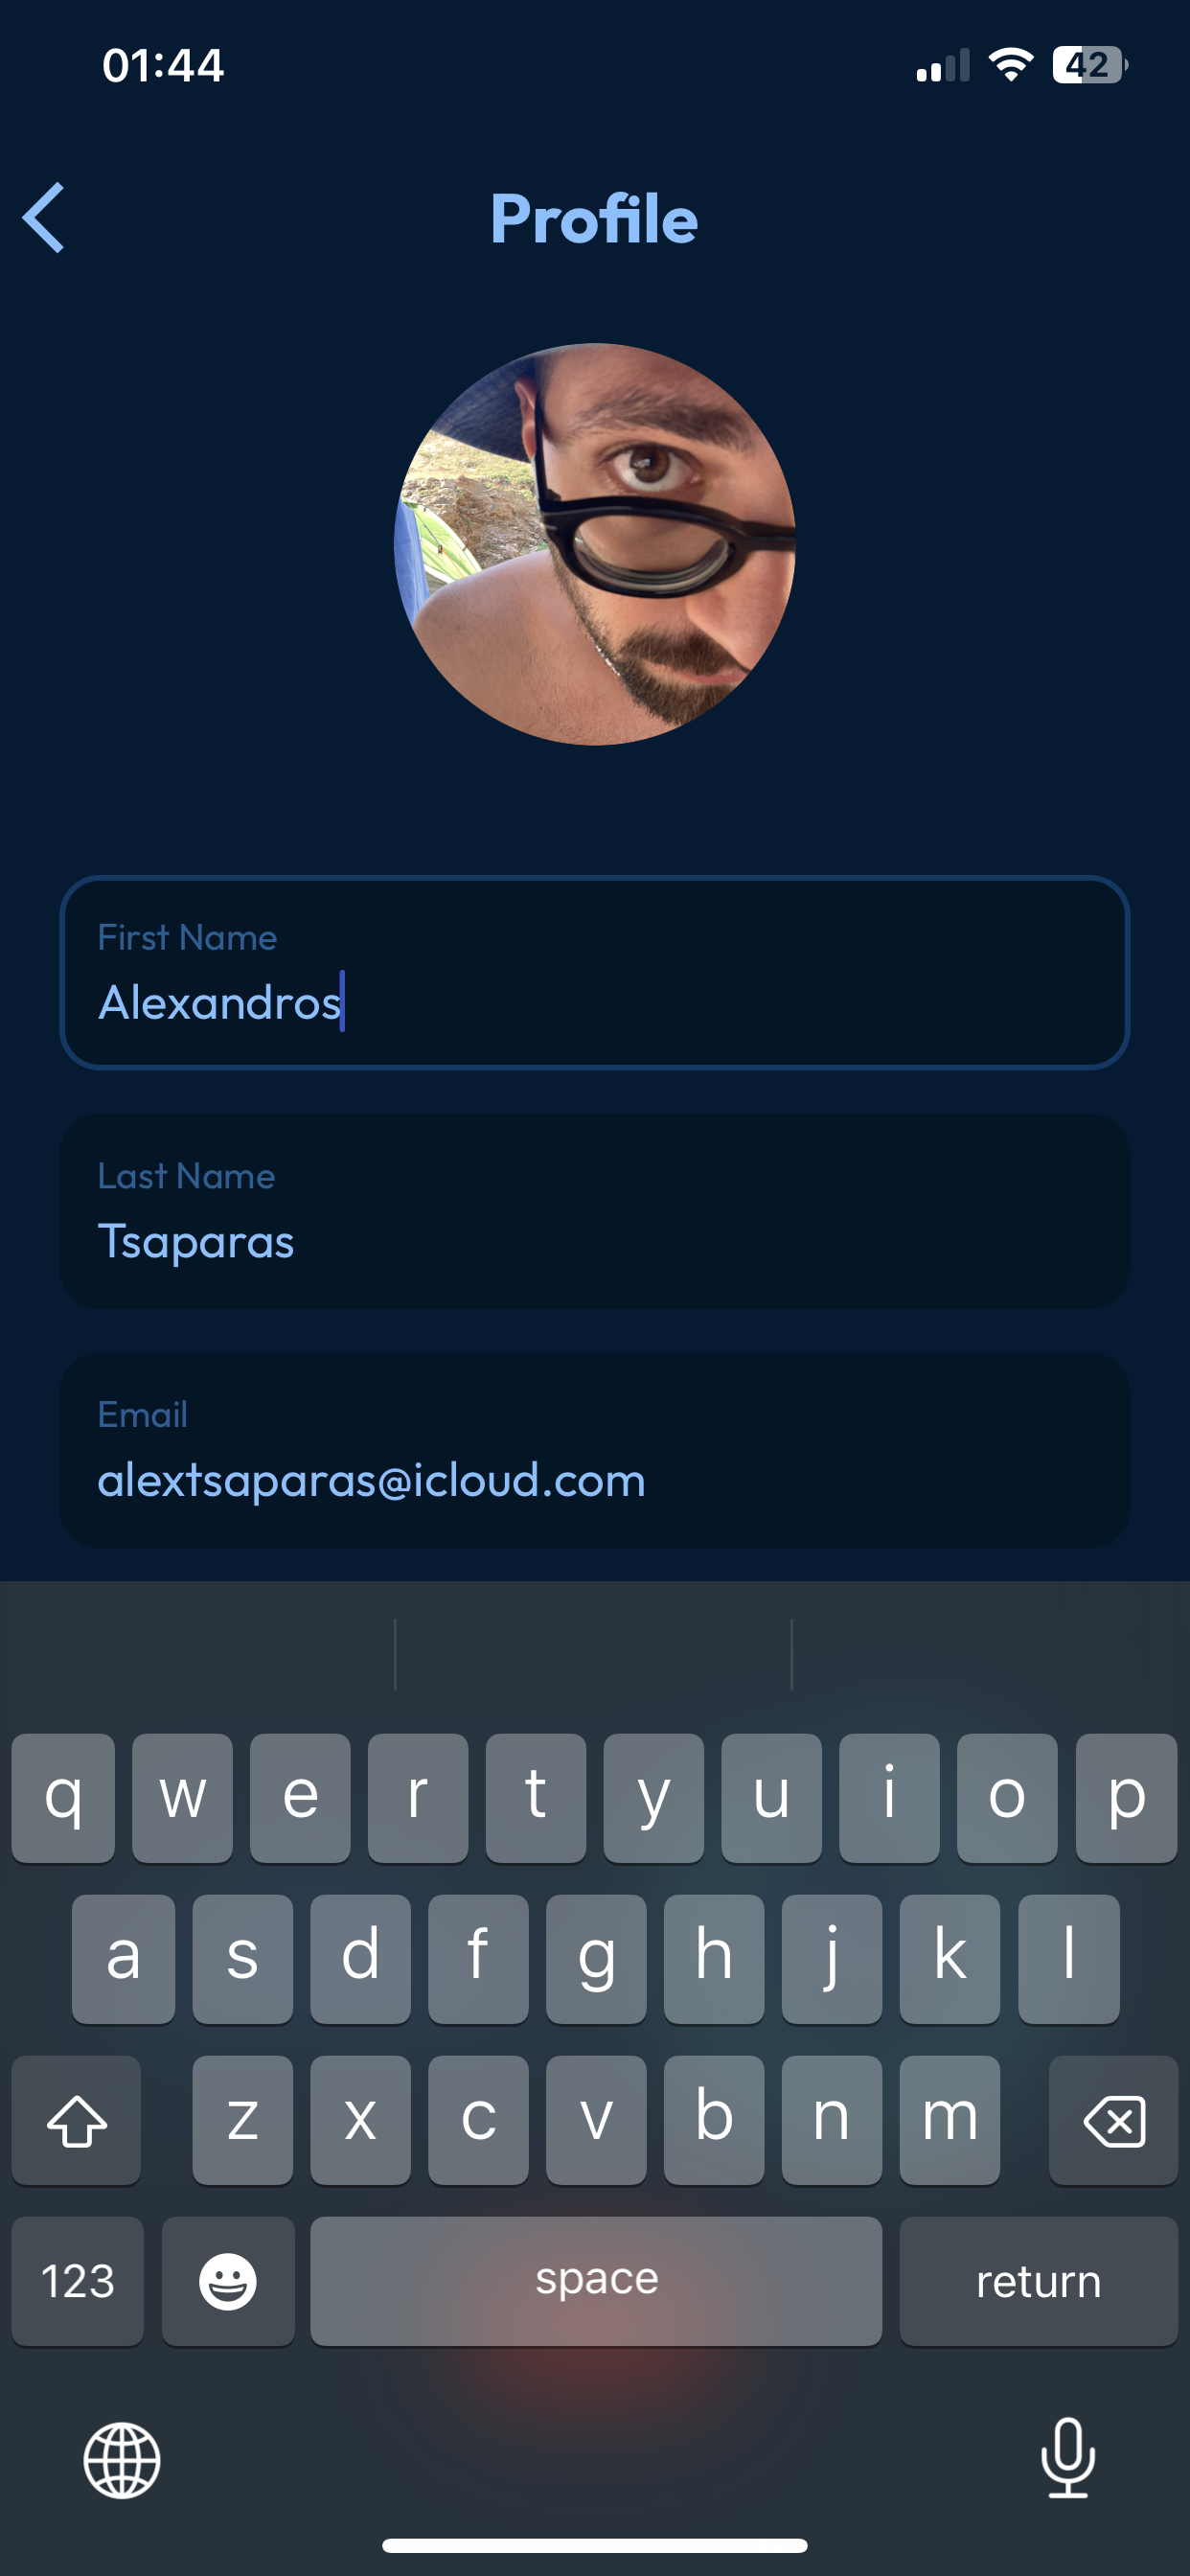
\includegraphics[scale=0.11]{figures/screenshots/Update User Info/2.PNG}\label{fig:user-info-step-2}}
    \hfill
    \subfloat[Step 3]{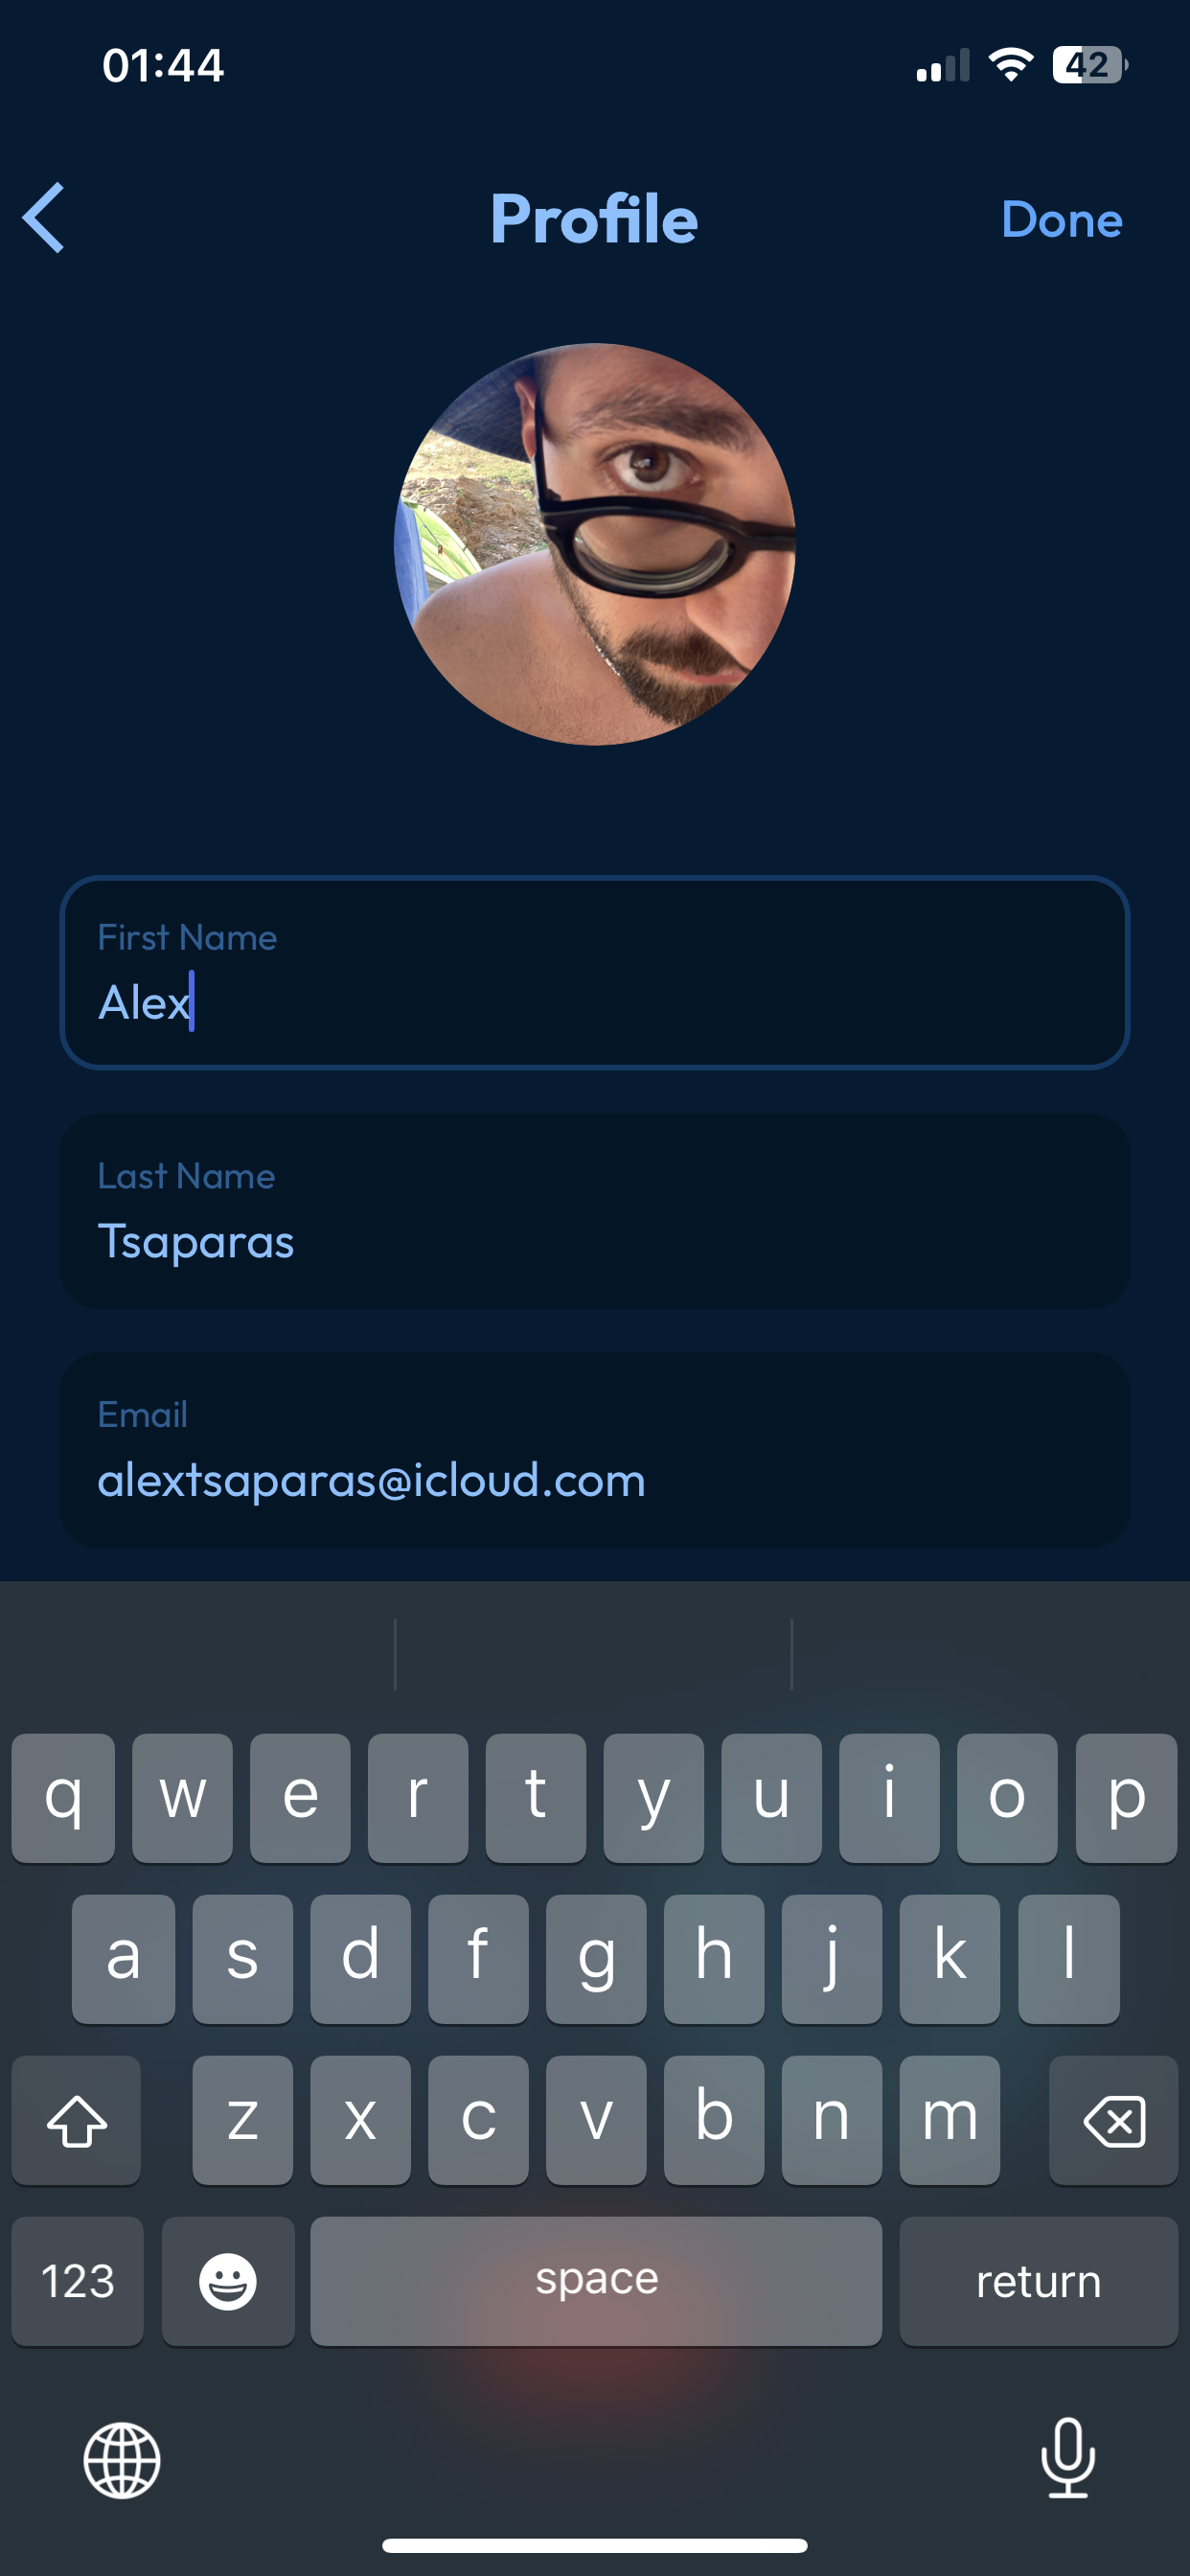
\includegraphics[scale=0.11]{figures/screenshots/Update User Info/3.PNG}\label{fig:user-info-step-3}}
    \hspace{2mm}
    \subfloat[Step 4]{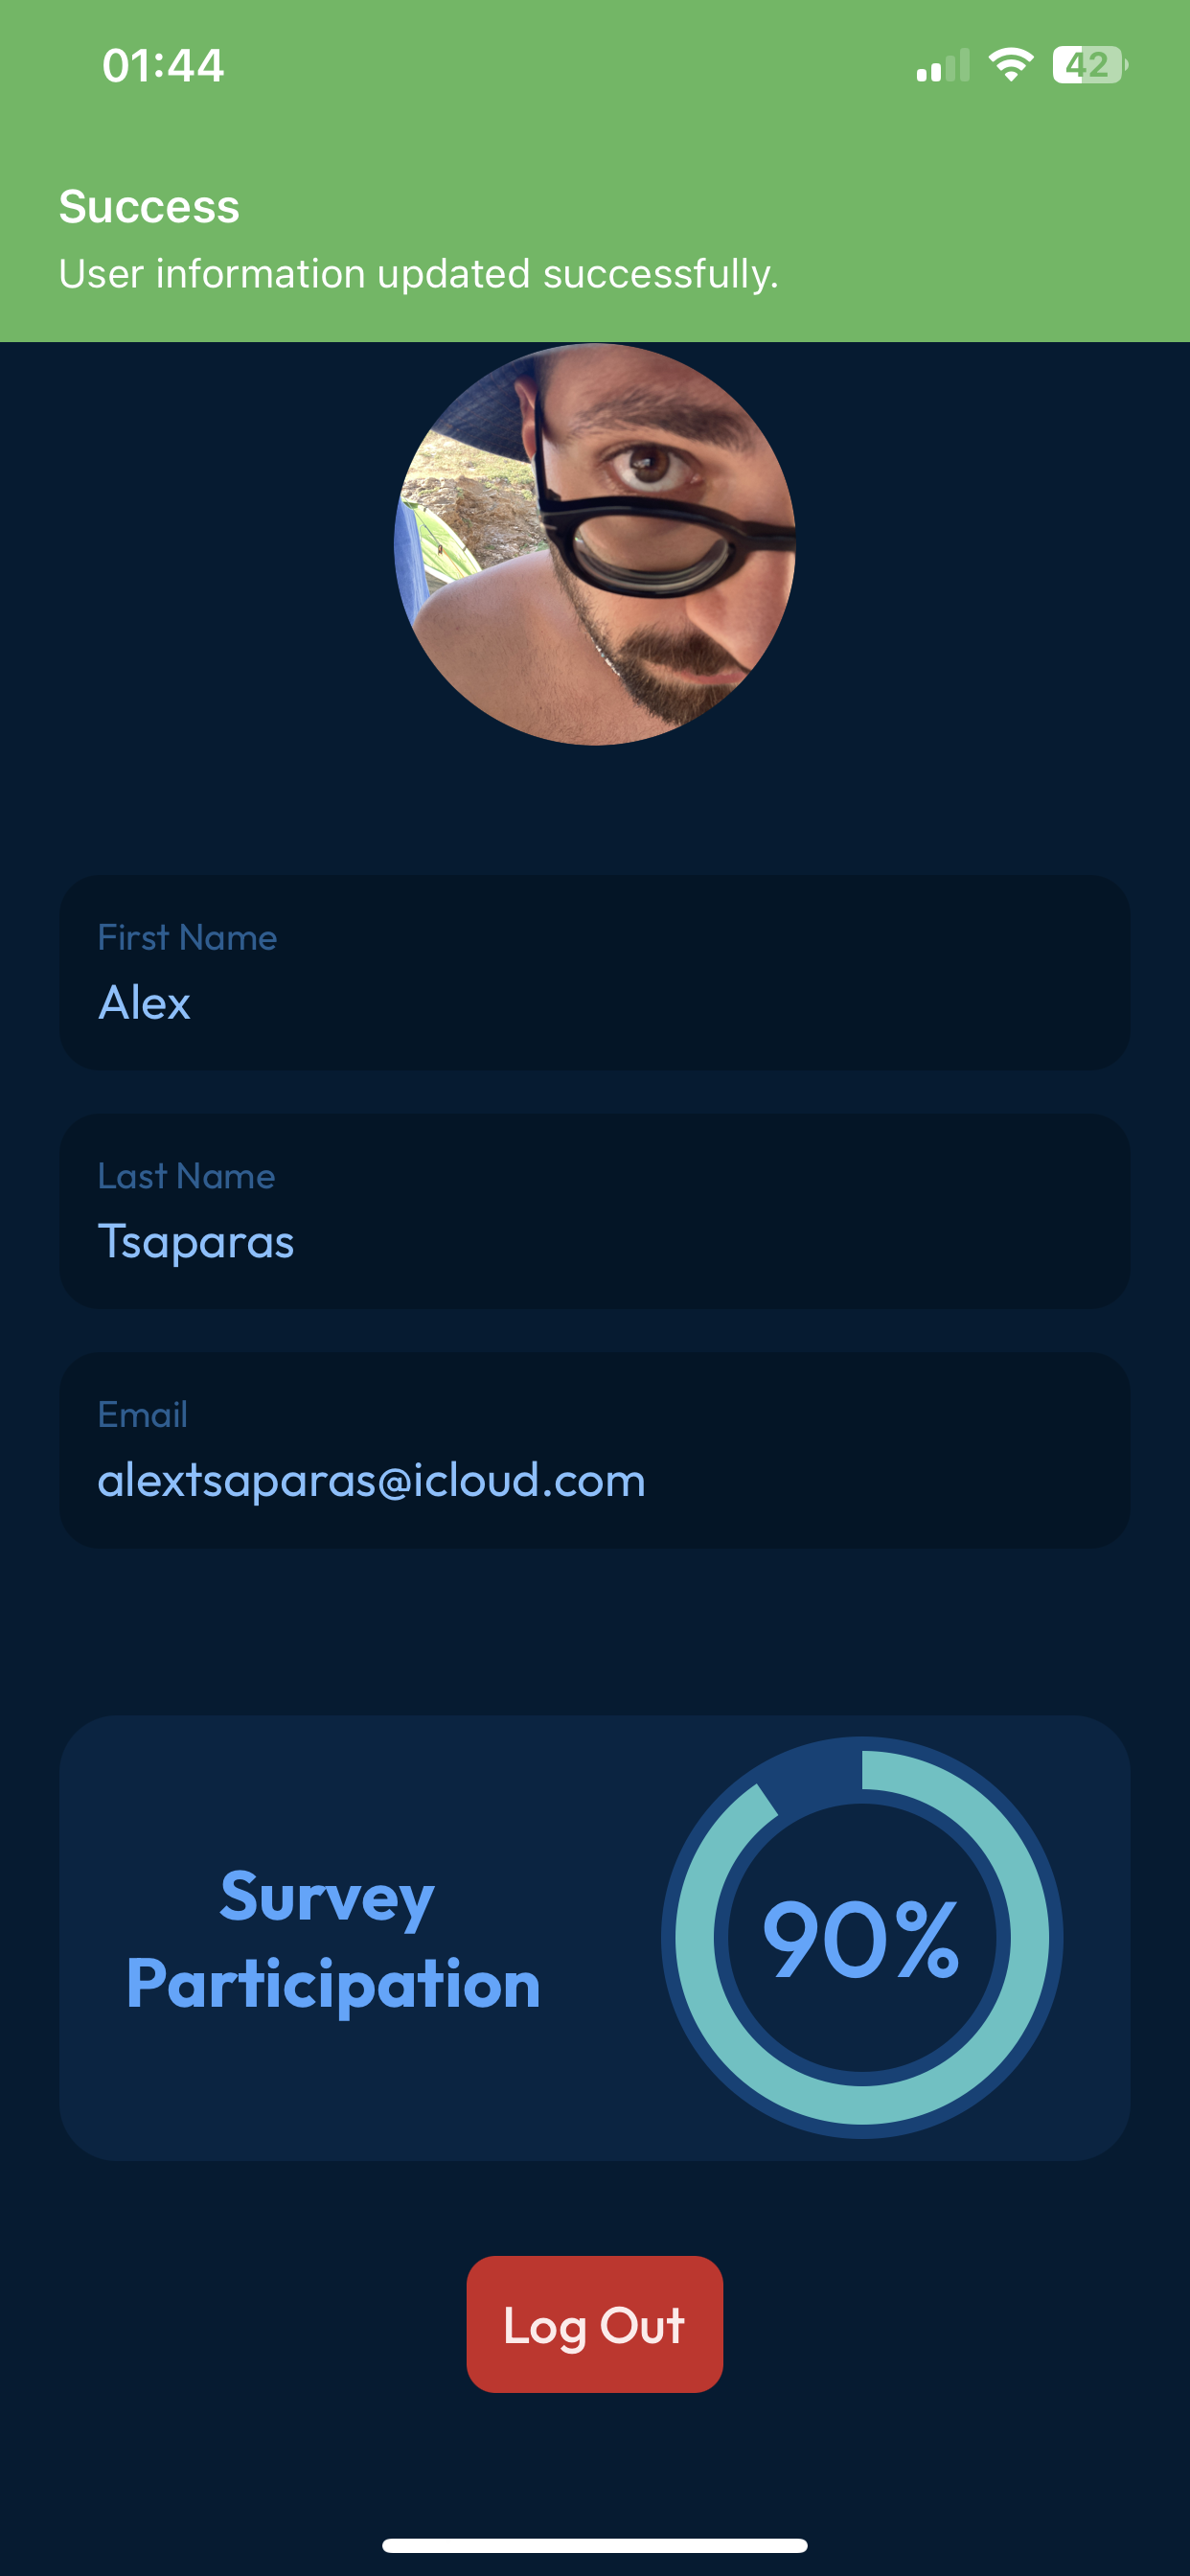
\includegraphics[scale=0.11]{figures/screenshots/Update User Info/4.PNG}\label{fig:user-info-step-4}}
    \caption{Procedure - Update the user's First Name}
\end{figure}
\FloatBarrier

\section{Deployment}

The deployment process was handled separately for the front-end and back-end, both utilizing \textbf{\href{https://cloud.google.com/?hl=en}{Google Cloud}}\footnote{Link: \url{https://cloud.google.com/?hl=en}} as the hosting environment. Google Cloud provides a comprehensive suite of cloud services, enabling robust, scalable, and secure deployment of applications. With its flexible infrastructure, we were able to deploy both the front-end and back-end using Virtual Machines (VMs), ensuring high availability and easy management. Moreover, Google Cloud offers a free trial with \$300 in free credits that can be used over a period of three months, making it an ideal option for experimenting and testing projects like this one without incurring initial costs. This trial is particularly beneficial for setting up virtual machines and testing deployments, helping to manage expenses effectively during the development and testing phases.

\subsection{Google Cloud Platform}

Google Cloud is a powerful cloud computing service that offers infrastructure as a service (IaaS), platform as a service (PaaS), and serverless computing environments. It supports various programming languages and frameworks, making it an ideal choice for hosting diverse applications. By using Google Cloud, we benefit from global scalability, strong security protocols, and comprehensive monitoring tools that aid in managing and optimizing the performance of the application.

\subsection{Front-end Deployment}

For the front-end deployment, we created a dedicated virtual machine named \textbf{moodtracker-application-vm}. The following steps outline the deployment process for the front-end:

\begin{enumerate}
    \item \textbf{VM Setup}: A virtual machine was created to host the front-end application, and the code repository was cloned onto this machine, using: \begin{verbatim} git clone https://github.com/tsaperlein/MoodTracker.git \end{verbatim}
    \item \textbf{Installing Dependencies}: Once inside the VM, the necessary npm packages were installed using: \begin{verbatim} npm install \end{verbatim}
    \item \textbf{Starting the Application}: The front-end was launched using the command: \begin{verbatim} npx expo start –-tunnel \end{verbatim}
    This command is essential for making the app accessible from any network, allowing test users to access it using a QR code or URL link.
    \item \textbf{Managing the Process}: To keep the application running continuously, the \textbf{\href{https://pm2.keymetrics.io/}{PM2}}\footnote{Link: \url{https://pm2.keymetrics.io/}} library was used. PM2 is a process manager for Node.js applications, which helps run the app persistently in the background and ensures that it maintains the same URL and QR code, even if the VM restarts. To install it we run: \begin{verbatim} npm install pm2 -g \end{verbatim}
    \item \textbf{Running the project using PM2}: In order to run the project we have to use the command: \begin{verbatim} pm2 start "npx expo start --tunnel" \end{verbatim}
    This process saves our running project in the library's list, and we could see it by running: \begin{verbatim} pm2 list \end{verbatim}
    \item \textbf{Handling URL Expiration}: One limitation to note is that Expo occasionally updates the URL, typically every two weeks, which might require re-sharing the link with test users. However, for the testing phase, this setup is very efficient and user-friendly.
\end{enumerate}

\subsection{Back-end Deployment}

For the back-end, another virtual machine named \textbf{moodtracker-api-vm} was used. This time, Docker was utilized to containerize the back-end application. Docker is a platform that automates the deployment of applications inside lightweight containers, providing a consistent environment regardless of where the code is executed. Using Docker simplifies deployment by packaging the application with all its dependencies, ensuring it runs reliably across different computing environments.\vspace{5mm} \\
The steps that we follow for Back-end Deployment:

\begin{enumerate}
    \item \textbf{Creating a Dockerfile}: A `Dockerfile' was constructed to define the image for the back-end application. It includes instructions for setting up the Node.js environment, installing dependencies, copying application files, and exposing the appropriate ports. The Dockerfile contents are as follows:
    
    \vspace{5mm}
    
\begin{lstlisting}[caption={Back-end Dockerfile}]
# Use an official Node.js runtime as a parent image
FROM node:22

# Set the working directory inside the container
WORKDIR /src

# Copy package.json and package-lock.json files to the working directory
COPY package.json package.json
COPY package-lock.json package-lock.json

# Install dependencies
RUN npm install

# Copy the rest of the application files to the working directory
COPY . .

# Expose the port your app runs on (adjust this to the actual port if different)
EXPOSE 3000

# Define the command to run your app in development mode
CMD ["npm", "run", "start:dev"]
\end{lstlisting}        

    \vspace{5mm}
        
    \item \textbf{Building and Saving the Docker Image}: The Docker image was built using the command: \begin{verbatim} docker build -t moodtracker-api \end{verbatim}
    Once built, the image was saved as a tar file using: \begin{verbatim} docker save -o moodtracker-api.tar moodtracker-api \end{verbatim}
    
    \item \textbf{Transferring the Image to the VM}: The tar file was transferred to the virtual machine using the command: \begin{verbatim} scp ./moodtracker-api.tar <username_google_cloud>@
        <vm_external_ip_address>:~/ \end{verbatim}
    
    \item \textbf{Loading the Docker Image in the VM}: After accessing the VM via SSH, the image was loaded using the command: \begin{verbatim} docker load -i ~/moodtracker-api.tar \end{verbatim}
    
    \item \textbf{Running the Docker Container}: The Docker container was started using the command: \begin{verbatim} docker run -d -p 80:3000 moodtracker-api:latest \end{verbatim}
    This command maps the port 3000 of the container to port 80 of the VM, making the API accessible through the external IP address without specifying a port number.
\end{enumerate}

\noindent This setup ensures that the front-end can communicate with the back-end using the external IP address of the moodtracker-api-vm. This deployment strategy allows for easy scaling, management, and monitoring of both front-end and back-end services independently.


\section{Summary}

In this chapter, we thoroughly explored the process of developing and implementing the application, starting with database design and schema definition, followed by front-end and back-end development, and build up to key aspects such as project setup and API integration. We also conducted an in-depth application walkthrough to demonstrate the flow and functionality of the primary screens. Finally, we successfully deployed both the front-end and back-end using Google Cloud Platform, creating a stable environment for the application. With these implementations complete, we are prepared to move forward to the next step: evaluating the system’s performance through user testing to ensure seamless functionality.